% Options for packages loaded elsewhere
\PassOptionsToPackage{unicode}{hyperref}
\PassOptionsToPackage{hyphens}{url}
%
\documentclass[
  english,
  a4paper,
]{article}
\author{true \and true \and true \and true \and true}
\date{}

\usepackage{amsmath,amssymb}
\usepackage{lmodern}
\usepackage{iftex}
\ifPDFTeX
  \usepackage[T1]{fontenc}
  \usepackage[utf8]{inputenc}
  \usepackage{textcomp} % provide euro and other symbols
\else % if luatex or xetex
  \usepackage{unicode-math}
  \defaultfontfeatures{Scale=MatchLowercase}
  \defaultfontfeatures[\rmfamily]{Ligatures=TeX,Scale=1}
\fi
% Use upquote if available, for straight quotes in verbatim environments
\IfFileExists{upquote.sty}{\usepackage{upquote}}{}
\IfFileExists{microtype.sty}{% use microtype if available
  \usepackage[]{microtype}
  \UseMicrotypeSet[protrusion]{basicmath} % disable protrusion for tt fonts
}{}
\makeatletter
\@ifundefined{KOMAClassName}{% if non-KOMA class
  \IfFileExists{parskip.sty}{%
    \usepackage{parskip}
  }{% else
    \setlength{\parindent}{0pt}
    \setlength{\parskip}{6pt plus 2pt minus 1pt}}
}{% if KOMA class
  \KOMAoptions{parskip=half}}
\makeatother
\usepackage{xcolor}
\IfFileExists{xurl.sty}{\usepackage{xurl}}{} % add URL line breaks if available
\IfFileExists{bookmark.sty}{\usepackage{bookmark}}{\usepackage{hyperref}}
\hypersetup{
  pdflang={en},
  hidelinks,
  pdfcreator={LaTeX via pandoc}}
\urlstyle{same} % disable monospaced font for URLs
\usepackage[margin=1in]{geometry}
\usepackage{longtable,booktabs,array}
\usepackage{calc} % for calculating minipage widths
% Correct order of tables after \paragraph or \subparagraph
\usepackage{etoolbox}
\makeatletter
\patchcmd\longtable{\par}{\if@noskipsec\mbox{}\fi\par}{}{}
\makeatother
% Allow footnotes in longtable head/foot
\IfFileExists{footnotehyper.sty}{\usepackage{footnotehyper}}{\usepackage{footnote}}
\makesavenoteenv{longtable}
\usepackage{graphicx}
\makeatletter
\def\maxwidth{\ifdim\Gin@nat@width>\linewidth\linewidth\else\Gin@nat@width\fi}
\def\maxheight{\ifdim\Gin@nat@height>\textheight\textheight\else\Gin@nat@height\fi}
\makeatother
% Scale images if necessary, so that they will not overflow the page
% margins by default, and it is still possible to overwrite the defaults
% using explicit options in \includegraphics[width, height, ...]{}
\setkeys{Gin}{width=\maxwidth,height=\maxheight,keepaspectratio}
% Set default figure placement to htbp
\makeatletter
\def\fps@figure{htbp}
\makeatother
\setlength{\emergencystretch}{3em} % prevent overfull lines
\providecommand{\tightlist}{%
  \setlength{\itemsep}{0pt}\setlength{\parskip}{0pt}}
\setcounter{secnumdepth}{5}
\newlength{\cslhangindent}
\setlength{\cslhangindent}{1.5em}
\newlength{\csllabelwidth}
\setlength{\csllabelwidth}{3em}
\newlength{\cslentryspacingunit} % times entry-spacing
\setlength{\cslentryspacingunit}{\parskip}
\newenvironment{CSLReferences}[2] % #1 hanging-ident, #2 entry spacing
 {% don't indent paragraphs
  \setlength{\parindent}{0pt}
  % turn on hanging indent if param 1 is 1
  \ifodd #1
  \let\oldpar\par
  \def\par{\hangindent=\cslhangindent\oldpar}
  \fi
  % set entry spacing
  \setlength{\parskip}{#2\cslentryspacingunit}
 }%
 {}
\usepackage{calc}
\newcommand{\CSLBlock}[1]{#1\hfill\break}
\newcommand{\CSLLeftMargin}[1]{\parbox[t]{\csllabelwidth}{#1}}
\newcommand{\CSLRightInline}[1]{\parbox[t]{\linewidth - \csllabelwidth}{#1}\break}
\newcommand{\CSLIndent}[1]{\hspace{\cslhangindent}#1}
\usepackage{booktabs}
\usepackage{longtable}
\usepackage{array}
\usepackage{multirow}
\usepackage{wrapfig}
\usepackage{float}
\usepackage{colortbl}
\usepackage{pdflscape}
\usepackage{tabu}
\usepackage{threeparttable}
\usepackage[normalem]{ulem}
\usepackage{makecell}
\usepackage{xcolor}
\usepackage{placeins}
\ifXeTeX
  % Load polyglossia as late as possible: uses bidi with RTL langages (e.g. Hebrew, Arabic)
  \usepackage{polyglossia}
  \setmainlanguage[]{english}
\else
  \usepackage[main=english]{babel}
% get rid of language-specific shorthands (see #6817):
\let\LanguageShortHands\languageshorthands
\def\languageshorthands#1{}
\fi
\ifLuaTeX
  \usepackage{selnolig}  % disable illegal ligatures
\fi

\begin{document}

{
\setcounter{tocdepth}{2}
\tableofcontents
}
\newcommand\CapeM{$40^\circ 10^\prime N$}
\newcommand\PtC{$34^\circ 27^\prime N$}
\newcommand\CAOR{$42^\circ 00^\prime N$}

\newpage

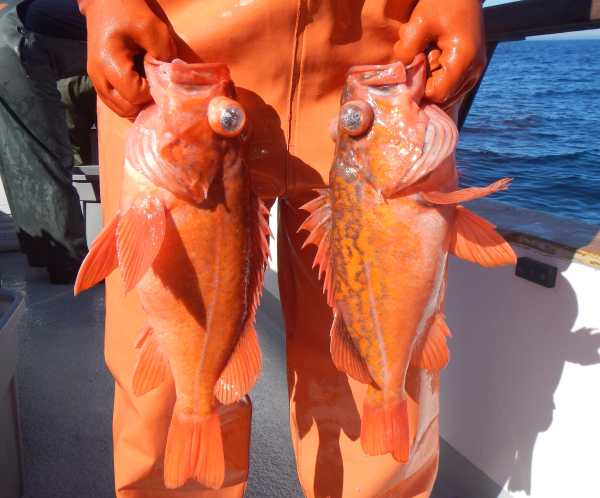
\includegraphics{cover_photo.png}
Two fish of the vermilion/sunset cryptic species pair. Confirmation of
species can only be determined via genetic analysis and species identification
of these two fish caught in the Santa Barbara channel at approximately 250 ft depth
is unknown. Photo courtesy of Sabrina Beyer.

\pagebreak
\pagenumbering{roman}
\setcounter{page}{1}

\renewcommand{\thetable}{\roman{table}}
\renewcommand{\thefigure}{\roman{figure}}

\setlength\parskip{0.5em plus 0.1em minus 0.2em}

\hypertarget{executive-summary}{%
\section*{Executive Summary}\label{executive-summary}}
\addcontentsline{toc}{section}{Executive Summary}

To be completed after the STAR panel. Tables from the pre-STAR base model
are included for reference during the STAR panel.

\hypertarget{stock}{%
\subsection*{Stock}\label{stock}}
\addcontentsline{toc}{subsection}{Stock}

This assessment reports the status of the vermlion rockfish (\emph{Sebastes miniatus})
and sunset rockfish (\emph{Sebastes crocotulus}) complex (referred to as vermilion
throughout), resource in U.S. waters off the coast of California south
of Point Conception ($34^\circ 27^\prime N$) using data through 2020.

\hypertarget{landings}{%
\subsection*{Landings}\label{landings}}
\addcontentsline{toc}{subsection}{Landings}

Text will be provided after the STAR panel.

\begin{table}[H]

\caption{\label{tab:removalsES}Recent landings by fleet, total landings summed across fleets, and the total mortality including discards.}
\centering
\resizebox{\linewidth}{!}{
\begin{tabular}[t]{rrrrrrrrr}
\toprule
Year & COM-HKL & COM-TWL & COM-NET & REC-PC & REC-PC-DIS & REC-PR & REC-PR-DIS & Total Landings\\
\midrule
\cellcolor{gray!6}{2011} & \cellcolor{gray!6}{10.047} & \cellcolor{gray!6}{0.000} & \cellcolor{gray!6}{0.000} & \cellcolor{gray!6}{39.917} & \cellcolor{gray!6}{0.297} & \cellcolor{gray!6}{49.164} & \cellcolor{gray!6}{0.147} & \cellcolor{gray!6}{99.573}\\
2012 & 9.400 & 0.006 & 0.000 & 35.709 & 0.246 & 40.881 & 0.230 & 86.471\\
\cellcolor{gray!6}{2013} & \cellcolor{gray!6}{13.845} & \cellcolor{gray!6}{0.005} & \cellcolor{gray!6}{0.000} & \cellcolor{gray!6}{20.975} & \cellcolor{gray!6}{0.121} & \cellcolor{gray!6}{40.398} & \cellcolor{gray!6}{0.123} & \cellcolor{gray!6}{75.467}\\
2014 & 14.139 & 0.015 & 0.023 & 21.006 & 0.042 & 41.537 & 0.214 & 76.976\\
\cellcolor{gray!6}{2015} & \cellcolor{gray!6}{18.172} & \cellcolor{gray!6}{0.410} & \cellcolor{gray!6}{0.010} & \cellcolor{gray!6}{39.781} & \cellcolor{gray!6}{0.102} & \cellcolor{gray!6}{64.386} & \cellcolor{gray!6}{0.210} & \cellcolor{gray!6}{123.071}\\
\addlinespace
2016 & 13.271 & 0.094 & 0.000 & 37.105 & 0.179 & 59.669 & 0.244 & 110.562\\
\cellcolor{gray!6}{2017} & \cellcolor{gray!6}{14.226} & \cellcolor{gray!6}{0.062} & \cellcolor{gray!6}{0.002} & \cellcolor{gray!6}{92.562} & \cellcolor{gray!6}{0.375} & \cellcolor{gray!6}{59.228} & \cellcolor{gray!6}{0.272} & \cellcolor{gray!6}{166.728}\\
2018 & 19.041 & 0.619 & 0.000 & 87.305 & 0.148 & 72.522 & 0.252 & 179.887\\
\cellcolor{gray!6}{2019} & \cellcolor{gray!6}{19.593} & \cellcolor{gray!6}{0.039} & \cellcolor{gray!6}{0.000} & \cellcolor{gray!6}{90.417} & \cellcolor{gray!6}{0.318} & \cellcolor{gray!6}{91.273} & \cellcolor{gray!6}{0.647} & \cellcolor{gray!6}{202.288}\\
2020 & 19.930 & 0.017 & 0.000 & 54.210 & 0.166 & 63.115 & 0.276 & 137.715\\
\bottomrule
\end{tabular}}
\end{table}

\hypertarget{data-and-assessment}{%
\subsection*{Data and Assessment}\label{data-and-assessment}}
\addcontentsline{toc}{subsection}{Data and Assessment}

Text will be provided after the STAR panel.

\hypertarget{stock-biomass}{%
\subsection*{Stock Biomass}\label{stock-biomass}}
\addcontentsline{toc}{subsection}{Stock Biomass}

Text will be provided after the STAR panel.

\begin{table}[H]

\caption{\label{tab:ssbES}Estimated recent trend in spawning output and the fraction unfished and the 95 percent intervals.}
\centering
\resizebox{\linewidth}{!}{
\begin{tabular}[t]{rrrrrrr}
\toprule
Year & Spawning Output & Lower Interval & Upper Interval & Fraction Unfished & Lower Interval & Upper Interval\\
\midrule
\cellcolor{gray!6}{2011} & \cellcolor{gray!6}{374.553} & \cellcolor{gray!6}{206.133} & \cellcolor{gray!6}{542.973} & \cellcolor{gray!6}{0.336} & \cellcolor{gray!6}{0.193} & \cellcolor{gray!6}{0.479}\\
2012 & 376.215 & 205.474 & 546.956 & 0.338 & 0.193 & 0.482\\
\cellcolor{gray!6}{2013} & \cellcolor{gray!6}{381.751} & \cellcolor{gray!6}{208.326} & \cellcolor{gray!6}{555.176} & \cellcolor{gray!6}{0.342} & \cellcolor{gray!6}{0.196} & \cellcolor{gray!6}{0.489}\\
2014 & 392.150 & 214.998 & 569.302 & 0.352 & 0.203 & 0.501\\
\cellcolor{gray!6}{2015} & \cellcolor{gray!6}{406.051} & \cellcolor{gray!6}{224.071} & \cellcolor{gray!6}{588.031} & \cellcolor{gray!6}{0.364} & \cellcolor{gray!6}{0.211} & \cellcolor{gray!6}{0.517}\\
\addlinespace
2016 & 415.346 & 228.219 & 602.473 & 0.373 & 0.215 & 0.530\\
\cellcolor{gray!6}{2017} & \cellcolor{gray!6}{425.372} & \cellcolor{gray!6}{233.255} & \cellcolor{gray!6}{617.489} & \cellcolor{gray!6}{0.382} & \cellcolor{gray!6}{0.220} & \cellcolor{gray!6}{0.543}\\
2018 & 424.535 & 227.829 & 621.241 & 0.381 & 0.216 & 0.546\\
\cellcolor{gray!6}{2019} & \cellcolor{gray!6}{422.707} & \cellcolor{gray!6}{221.342} & \cellcolor{gray!6}{624.072} & \cellcolor{gray!6}{0.379} & \cellcolor{gray!6}{0.210} & \cellcolor{gray!6}{0.548}\\
2020 & 421.587 & 214.783 & 628.391 & 0.378 & 0.204 & 0.552\\
\addlinespace
\cellcolor{gray!6}{2021} & \cellcolor{gray!6}{436.090} & \cellcolor{gray!6}{221.701} & \cellcolor{gray!6}{650.479} & \cellcolor{gray!6}{0.391} & \cellcolor{gray!6}{0.210} & \cellcolor{gray!6}{0.572}\\
\bottomrule
\end{tabular}}
\end{table}

\hypertarget{recruitment}{%
\subsection*{Recruitment}\label{recruitment}}
\addcontentsline{toc}{subsection}{Recruitment}

Text will be provided after the STAR panel.

\begin{table}[H]

\caption{\label{tab:recrES}Estimated recent trend in recruitment and recruitment deviations and the 95 percent intervals.}
\centering
\resizebox{\linewidth}{!}{
\begin{tabular}[t]{rrrrrrr}
\toprule
Year & Recruitment & Lower Interval & Upper Interval & Recruitment Deviations & Lower Interval & Upper Interval\\
\midrule
\cellcolor{gray!6}{2011} & \cellcolor{gray!6}{230.871} & \cellcolor{gray!6}{115.936} & \cellcolor{gray!6}{459.748} & \cellcolor{gray!6}{-0.375} & \cellcolor{gray!6}{-0.956} & \cellcolor{gray!6}{0.206}\\
2012 & 371.157 & 189.416 & 727.276 & 0.098 & -0.460 & 0.657\\
\cellcolor{gray!6}{2013} & \cellcolor{gray!6}{610.267} & \cellcolor{gray!6}{309.359} & \cellcolor{gray!6}{1203.863} & \cellcolor{gray!6}{0.592} & \cellcolor{gray!6}{0.026} & \cellcolor{gray!6}{1.158}\\
2014 & 674.358 & 328.949 & 1382.458 & 0.686 & 0.069 & 1.303\\
\cellcolor{gray!6}{2015} & \cellcolor{gray!6}{374.409} & \cellcolor{gray!6}{159.924} & \cellcolor{gray!6}{876.556} & \cellcolor{gray!6}{0.080} & \cellcolor{gray!6}{-0.701} & \cellcolor{gray!6}{0.860}\\
\addlinespace
2016 & 1764.000 & 916.754 & 3394.255 & 1.604 & 1.081 & 2.126\\
\cellcolor{gray!6}{2017} & \cellcolor{gray!6}{164.262} & \cellcolor{gray!6}{63.748} & \cellcolor{gray!6}{423.259} & \cellcolor{gray!6}{-0.796} & \cellcolor{gray!6}{-1.699} & \cellcolor{gray!6}{0.106}\\
2018 & 389.205 & 142.731 & 1061.303 & 0.046 & -0.929 & 1.020\\
\cellcolor{gray!6}{2019} & \cellcolor{gray!6}{382.875} & \cellcolor{gray!6}{140.496} & \cellcolor{gray!6}{1043.401} & \cellcolor{gray!6}{0.023} & \cellcolor{gray!6}{-0.949} & \cellcolor{gray!6}{0.996}\\
2020 & 380.347 & 139.774 & 1034.984 & 0.017 & -0.952 & 0.987\\
\addlinespace
\cellcolor{gray!6}{2021} & \cellcolor{gray!6}{376.582} & \cellcolor{gray!6}{140.492} & \cellcolor{gray!6}{1009.410} & \cellcolor{gray!6}{0.000} & \cellcolor{gray!6}{-0.980} & \cellcolor{gray!6}{0.980}\\
\bottomrule
\end{tabular}}
\end{table}

\hypertarget{exploitation-status}{%
\subsection*{Exploitation Status}\label{exploitation-status}}
\addcontentsline{toc}{subsection}{Exploitation Status}

Text will be provided after the STAR panel.

\begin{table}[H]

\caption{\label{tab:exploitES}Estimated recent trend in the (1-SPR)/(1-SPR 50\%) where SPR is the spawning potential ratio the exploitation rate, and the  95 percent intervals.}
\centering
\resizebox{\linewidth}{!}{
\begin{tabular}[t]{rrrrrrr}
\toprule
Year & (1-SPR)/(1-SPR 50\%) & Lower Interval & Upper Interval & Exploitation Rate & Lower Interval & Upper Interval\\
\midrule
\cellcolor{gray!6}{2011} & \cellcolor{gray!6}{1.004} & \cellcolor{gray!6}{0.697} & \cellcolor{gray!6}{1.311} & \cellcolor{gray!6}{0.066} & \cellcolor{gray!6}{0.039} & \cellcolor{gray!6}{0.094}\\
2012 & 0.885 & 0.592 & 1.177 & 0.055 & 0.032 & 0.078\\
\cellcolor{gray!6}{2013} & \cellcolor{gray!6}{0.770} & \cellcolor{gray!6}{0.499} & \cellcolor{gray!6}{1.041} & \cellcolor{gray!6}{0.044} & \cellcolor{gray!6}{0.026} & \cellcolor{gray!6}{0.062}\\
2014 & 0.755 & 0.490 & 1.020 & 0.043 & 0.026 & 0.061\\
\cellcolor{gray!6}{2015} & \cellcolor{gray!6}{1.027} & \cellcolor{gray!6}{0.722} & \cellcolor{gray!6}{1.331} & \cellcolor{gray!6}{0.067} & \cellcolor{gray!6}{0.040} & \cellcolor{gray!6}{0.095}\\
\addlinespace
2016 & 0.954 & 0.656 & 1.253 & 0.061 & 0.036 & 0.086\\
\cellcolor{gray!6}{2017} & \cellcolor{gray!6}{1.168} & \cellcolor{gray!6}{0.849} & \cellcolor{gray!6}{1.487} & \cellcolor{gray!6}{0.087} & \cellcolor{gray!6}{0.048} & \cellcolor{gray!6}{0.125}\\
2018 & 1.212 & 0.890 & 1.535 & 0.091 & 0.050 & 0.132\\
\cellcolor{gray!6}{2019} & \cellcolor{gray!6}{1.277} & \cellcolor{gray!6}{0.954} & \cellcolor{gray!6}{1.600} & \cellcolor{gray!6}{0.102} & \cellcolor{gray!6}{0.055} & \cellcolor{gray!6}{0.148}\\
2020 & 1.007 & 0.680 & 1.334 & 0.065 & 0.035 & 0.095\\
\bottomrule
\end{tabular}}
\end{table}

\hypertarget{reference-points}{%
\subsection*{Reference Points}\label{reference-points}}
\addcontentsline{toc}{subsection}{Reference Points}

Text will be provided after the STAR panel.

\begin{table}[H]

\caption{\label{tab:referenceES}Summary of reference points and management quantities including estimates of the 95 percent intervals.}
\centering
\begin{tabular}[t]{lrrr}
\toprule
 & Estimate & Lower Interval & Upper Interval\\
\midrule
\cellcolor{gray!6}{Unfished Spawning Output} & \cellcolor{gray!6}{1114.670} & \cellcolor{gray!6}{885.848} & \cellcolor{gray!6}{1343.492}\\
Unfished Age 4+ Biomass (mt) & 6144.610 & 5491.397 & 6797.823\\
\cellcolor{gray!6}{Unfished Recruitment (R0)} & \cellcolor{gray!6}{433.531} & \cellcolor{gray!6}{306.058} & \cellcolor{gray!6}{561.004}\\
Spawning Output (2021) & 436.090 & 221.701 & 650.479\\
\cellcolor{gray!6}{Fraction Unfished (2021)} & \cellcolor{gray!6}{0.391} & \cellcolor{gray!6}{0.210} & \cellcolor{gray!6}{0.572}\\
\addlinespace
Reference Points Based SB40\% &  &  & \\
\cellcolor{gray!6}{Proxy Spawning Output SB40\%} & \cellcolor{gray!6}{445.868} & \cellcolor{gray!6}{354.339} & \cellcolor{gray!6}{537.397}\\
SPR Resulting in SB40\% & 0.458 & 0.458 & 0.458\\
\cellcolor{gray!6}{Exploitation Rate Resulting in SB40\%} & \cellcolor{gray!6}{0.074} & \cellcolor{gray!6}{0.061} & \cellcolor{gray!6}{0.087}\\
Yield with SPR Based On SB40\% (mt) & 147.732 & 125.913 & 169.551\\
\addlinespace
\cellcolor{gray!6}{Reference Points Based on SPR Proxy for MSY} & \cellcolor{gray!6}{} & \cellcolor{gray!6}{} & \cellcolor{gray!6}{}\\
Proxy Spawning Output (SPR50) & 497.314 & 395.224 & 599.404\\
\cellcolor{gray!6}{SPR50} & \cellcolor{gray!6}{0.500} & \cellcolor{gray!6}{} & \cellcolor{gray!6}{}\\
Exploitation Rate Corresponding to SPR50 & 0.065 & 0.053 & 0.076\\
\cellcolor{gray!6}{Yield with SPR50 at SB SPR (mt)} & \cellcolor{gray!6}{140.884} & \cellcolor{gray!6}{120.182} & \cellcolor{gray!6}{161.586}\\
\addlinespace
Reference Points Based on Estimated MSY Values &  &  & \\
\cellcolor{gray!6}{Spawning Output at MSY (SB MSY)} & \cellcolor{gray!6}{297.232} & \cellcolor{gray!6}{238.299} & \cellcolor{gray!6}{356.165}\\
SPR MSY & 0.338 & 0.329 & 0.347\\
\cellcolor{gray!6}{Exploitation Rate Corresponding to SPR MSY} & \cellcolor{gray!6}{0.109} & \cellcolor{gray!6}{0.090} & \cellcolor{gray!6}{0.128}\\
MSY (mt) & 157.796 & 134.005 & 181.587\\
\bottomrule
\end{tabular}
\end{table}

\hypertarget{management-performance}{%
\subsection*{Management Performance}\label{management-performance}}
\addcontentsline{toc}{subsection}{Management Performance}

Text will be provided after the STAR panel.

\begin{table}

\caption{\label{tab:management}Annual estimates of total mortality, overfishing limit (OFL), acceptable biological catch (ABC), annual catch limit (ACL) for vermilion. The ABC is equal to the ACL.  Data were obtained from the GEMM reports.}
\centering
\resizebox{\linewidth}{!}{
\begin{tabular}[t]{lrrrrrrrrrrrr}
\toprule
 & 2011 & 2012 & 2013 & 2014 & 2015 & 2016 & 2017 & 2018 & 2019 & 2020 & 2021 & 2022\\
\midrule
\addlinespace[0.3em]
\multicolumn{13}{l}{\textbf{North of 40°10' N}}\\
\hspace{1em}OFL & 11.127 & 11.127 & 9.717 & 9.717 & 9.717 & 9.717 & 9.720 & 9.720 & 9.720 & 9.720 & 9.700 & 9.700\\
\hspace{1em}ABC & 5.564 & 5.564 & 8.104 & 8.104 & 8.104 & 8.104 & 8.104 & 8.104 & 8.104 & 8.104 & 7.547 & 7.547\\
\hspace{1em}Total landings & 15.249 & 18.695 & 14.149 & 10.504 & 13.472 & 12.104 & 20.602 & 22.949 & 25.696 &  &  & \\
\hspace{1em}CA rec landings & 4.209 & 4.867 & 2.657 & 2.950 & 5.018 & 4.549 & 6.490 & 7.631 & 7.884 &  &  & \\
\hspace{1em}OR rec landings & 6.102 & 9.150 & 6.305 & 3.949 & 4.653 & 3.689 & 8.798 & 9.199 & 9.252 &  &  & \\
\hspace{1em}WA rec landings & 1.001 & 0.911 & 1.279 & 0.960 & 1.141 & 0.997 & 0.731 & 1.151 & 2.497 &  &  & \\
\hspace{1em}Commercial landings & 3.935 & 3.767 & 3.906 & 2.644 & 2.661 & 2.799 & 4.557 & 4.966 & 6.063 &  &  & \\
\hspace{1em}Research & 0.002 &  & 0.002 & 0.002 &  & 0.069 & 0.026 & 0.002 &  &  &  & \\
\addlinespace[0.3em]
\multicolumn{13}{l}{\textbf{South of 40°10' N}}\\
\hspace{1em}OFL & 308.359 & 308.359 & 269.276 & 269.276 & 269.276 & 269.276 & 269.280 & 269.280 & 269.280 & 269.280 & 269.280 & 269.280\\
\hspace{1em}ABC & 154.179 & 154.179 & 224.576 & 224.576 & 224.576 & 224.576 & 224.580 & 224.580 & 224.580 & 224.580 & 209.515 & 209.515\\
\hspace{1em}Total Landings & 210.310 & 235.216 & 237.074 & 197.043 & 334.984 & 292.375 & 341.207 & 344.454 & 484.967 &  &  & \\
\hspace{1em}CA rec landings & 191.437 & 216.480 & 208.198 & 167.572 & 291.779 & 260.162 & 287.493 & 278.158 & 413.946 &  &  & \\
\hspace{1em}Commercial landings & 16.928 & 16.642 & 26.601 & 26.607 & 39.669 & 29.148 & 48.195 & 59.644 & 67.189 &  &  & \\
\hspace{1em}Research & 1.944 & 2.094 & 2.275 & 2.863 & 3.536 & 3.065 & 5.519 & 6.652 & 3.832 &  &  & \\
\bottomrule
\end{tabular}}
\end{table}

\hypertarget{unresolved-problems-and-major-uncertainties}{%
\subsection*{Unresolved Problems and Major Uncertainties}\label{unresolved-problems-and-major-uncertainties}}
\addcontentsline{toc}{subsection}{Unresolved Problems and Major Uncertainties}

Text will be provided after the STAR panel.

\hypertarget{decision-table}{%
\subsection*{Decision Table}\label{decision-table}}
\addcontentsline{toc}{subsection}{Decision Table}

Text will be provided after the STAR panel.

\emph{Projections}

\begin{table}[H]

\caption{\label{tab:projectionES}Projections of potential OFLs (mt), ABCs (mt), estimated spawning output and fraction unfished.}
\centering
\resizebox{\linewidth}{!}{
\begin{tabular}[t]{rrrrrr}
\toprule
Year & Predicted OFL (mt) & ABC Catch (mt) & Age 4+ Biomass (mt) & Spawning Output & Fraction Unfished\\
\midrule
\cellcolor{gray!6}{2021} & \cellcolor{gray!6}{147.794} & \cellcolor{gray!6}{146.714} & \cellcolor{gray!6}{3400.59} & \cellcolor{gray!6}{436.090} & \cellcolor{gray!6}{0.391228}\\
2022 & 159.714 & 159.714 & 3527.33 & 458.465 & 0.411301\\
\cellcolor{gray!6}{2023} & \cellcolor{gray!6}{168.686} & \cellcolor{gray!6}{147.432} & \cellcolor{gray!6}{3611.43} & \cellcolor{gray!6}{485.754} & \cellcolor{gray!6}{0.435783}\\
2024 & 174.683 & 151.101 & 3678.42 & 515.410 & 0.462389\\
\cellcolor{gray!6}{2025} & \cellcolor{gray!6}{177.214} & \cellcolor{gray!6}{151.872} & \cellcolor{gray!6}{3714.99} & \cellcolor{gray!6}{540.924} & \cellcolor{gray!6}{0.485277}\\
\addlinespace
2026 & 177.252 & 150.487 & 3729.95 & 560.875 & 0.503176\\
\cellcolor{gray!6}{2027} & \cellcolor{gray!6}{175.790} & \cellcolor{gray!6}{147.840} & \cellcolor{gray!6}{3730.51} & \cellcolor{gray!6}{575.482} & \cellcolor{gray!6}{0.516281}\\
2028 & 173.625 & 144.630 & 3722.50 & 585.599 & 0.525357\\
\cellcolor{gray!6}{2029} & \cellcolor{gray!6}{171.299} & \cellcolor{gray!6}{141.493} & \cellcolor{gray!6}{3710.09} & \cellcolor{gray!6}{592.222} & \cellcolor{gray!6}{0.531298}\\
2030 & 169.121 & 138.341 & 3695.94 & 596.252 & 0.534914\\
\addlinespace
\cellcolor{gray!6}{2031} & \cellcolor{gray!6}{167.255} & \cellcolor{gray!6}{135.477} & \cellcolor{gray!6}{3682.04} & \cellcolor{gray!6}{598.492} & \cellcolor{gray!6}{0.536923}\\
2032 & 165.750 & 133.097 & 3669.45 & 599.548 & 0.537871\\
\bottomrule
\end{tabular}}
\end{table}

\emph{Summary Table}

\begin{table}[H]

\caption{\label{tab:summaryES}Summary of recent estimates and managment quantities.}
\centering
\resizebox{\linewidth}{!}{
\begin{tabular}[t]{lrrrrrrrrrrr}
\toprule
Quantity & 2011 & 2012 & 2013 & 2014 & 2015 & 2016 & 2017 & 2018 & 2019 & 2020 & 2021\\
\midrule
\cellcolor{gray!6}{OFL} & \cellcolor{gray!6}{11.127} & \cellcolor{gray!6}{11.127} & \cellcolor{gray!6}{9.717} & \cellcolor{gray!6}{9.717} & \cellcolor{gray!6}{9.717} & \cellcolor{gray!6}{9.717} & \cellcolor{gray!6}{9.720} & \cellcolor{gray!6}{9.720} & \cellcolor{gray!6}{9.720} & \cellcolor{gray!6}{9.720} & \cellcolor{gray!6}{9.700}\\
ABC & 5.564 & 5.564 & 8.104 & 8.104 & 8.104 & 8.104 & 8.104 & 8.104 & 8.104 & 8.104 & 7.547\\
\cellcolor{gray!6}{Total Catch} & \cellcolor{gray!6}{99.573} & \cellcolor{gray!6}{86.471} & \cellcolor{gray!6}{75.467} & \cellcolor{gray!6}{76.976} & \cellcolor{gray!6}{123.071} & \cellcolor{gray!6}{110.562} & \cellcolor{gray!6}{166.728} & \cellcolor{gray!6}{179.887} & \cellcolor{gray!6}{202.288} & \cellcolor{gray!6}{137.715} & \cellcolor{gray!6}{}\\
(1-SPR)/(1-SPR 50\%) & 1.004 & 0.885 & 0.770 & 0.755 & 1.027 & 0.954 & 1.168 & 1.212 & 1.277 & 1.007 & \\
\cellcolor{gray!6}{Fill in F method} & \cellcolor{gray!6}{0.066} & \cellcolor{gray!6}{0.055} & \cellcolor{gray!6}{0.044} & \cellcolor{gray!6}{0.043} & \cellcolor{gray!6}{0.067} & \cellcolor{gray!6}{0.061} & \cellcolor{gray!6}{0.087} & \cellcolor{gray!6}{0.091} & \cellcolor{gray!6}{0.102} & \cellcolor{gray!6}{0.065} & \cellcolor{gray!6}{}\\
\addlinespace
Age 4+ Biomass (mt) & 2399.000 & 2471.780 & 2608.110 & 2674.170 & 2722.320 & 2741.630 & 2833.670 & 2910.440 & 2921.780 & 3279.880 & 6138.760\\
\cellcolor{gray!6}{Spawning Output} & \cellcolor{gray!6}{374.553} & \cellcolor{gray!6}{376.215} & \cellcolor{gray!6}{381.751} & \cellcolor{gray!6}{392.150} & \cellcolor{gray!6}{406.051} & \cellcolor{gray!6}{415.346} & \cellcolor{gray!6}{425.372} & \cellcolor{gray!6}{424.535} & \cellcolor{gray!6}{422.707} & \cellcolor{gray!6}{421.587} & \cellcolor{gray!6}{436.090}\\
Lower Interval & 206.133 & 205.474 & 208.326 & 214.998 & 224.071 & 228.219 & 233.255 & 227.829 & 221.342 & 214.783 & 221.701\\
\cellcolor{gray!6}{Upper Interval} & \cellcolor{gray!6}{542.973} & \cellcolor{gray!6}{546.956} & \cellcolor{gray!6}{555.176} & \cellcolor{gray!6}{569.302} & \cellcolor{gray!6}{588.031} & \cellcolor{gray!6}{602.473} & \cellcolor{gray!6}{617.489} & \cellcolor{gray!6}{621.241} & \cellcolor{gray!6}{624.072} & \cellcolor{gray!6}{628.391} & \cellcolor{gray!6}{650.479}\\
Recruits & 230.871 & 371.157 & 610.267 & 674.358 & 374.409 & 1764.000 & 164.262 & 389.205 & 382.875 & 380.347 & 376.582\\
\addlinespace
\cellcolor{gray!6}{Lower Interval} & \cellcolor{gray!6}{115.936} & \cellcolor{gray!6}{189.416} & \cellcolor{gray!6}{309.359} & \cellcolor{gray!6}{328.949} & \cellcolor{gray!6}{159.924} & \cellcolor{gray!6}{916.754} & \cellcolor{gray!6}{63.748} & \cellcolor{gray!6}{142.731} & \cellcolor{gray!6}{140.496} & \cellcolor{gray!6}{139.774} & \cellcolor{gray!6}{140.492}\\
Upper Interval & 459.748 & 727.276 & 1203.863 & 1382.458 & 876.556 & 3394.255 & 423.259 & 1061.303 & 1043.401 & 1034.984 & 1009.410\\
\cellcolor{gray!6}{Fraction Unfished} & \cellcolor{gray!6}{0.336} & \cellcolor{gray!6}{0.338} & \cellcolor{gray!6}{0.342} & \cellcolor{gray!6}{0.352} & \cellcolor{gray!6}{0.364} & \cellcolor{gray!6}{0.373} & \cellcolor{gray!6}{0.382} & \cellcolor{gray!6}{0.381} & \cellcolor{gray!6}{0.379} & \cellcolor{gray!6}{0.378} & \cellcolor{gray!6}{0.391}\\
Lower Interval & 0.193 & 0.193 & 0.196 & 0.203 & 0.211 & 0.215 & 0.220 & 0.216 & 0.210 & 0.204 & 0.210\\
\cellcolor{gray!6}{Upper Interval} & \cellcolor{gray!6}{0.479} & \cellcolor{gray!6}{0.482} & \cellcolor{gray!6}{0.489} & \cellcolor{gray!6}{0.501} & \cellcolor{gray!6}{0.517} & \cellcolor{gray!6}{0.530} & \cellcolor{gray!6}{0.543} & \cellcolor{gray!6}{0.546} & \cellcolor{gray!6}{0.548} & \cellcolor{gray!6}{0.552} & \cellcolor{gray!6}{0.572}\\
\bottomrule
\end{tabular}}
\end{table}

\hypertarget{research-and-data-needs}{%
\subsection*{Research and Data Needs}\label{research-and-data-needs}}
\addcontentsline{toc}{subsection}{Research and Data Needs}

Text will be provided after the STAR panel.

\pagebreak
\setlength{\parskip}{5mm plus1mm minus1mm}
\pagenumbering{arabic}
\setcounter{page}{1}
\renewcommand{\thefigure}{\arabic{figure}}
\renewcommand{\thetable}{\arabic{table}}
\setcounter{table}{0}
\setcounter{figure}{0}

\hypertarget{introduction}{%
\section{Introduction}\label{introduction}}

Note to readers: Text in this section is the same in both California vermilion rockfish assessment
documents.

\hypertarget{basic-information-and-life-history}{%
\subsection{Basic Information and Life History}\label{basic-information-and-life-history}}

\emph{Note: Prior to the identification of sunset rockfish as a separate species (2008), historical studies of ``vermilion'' rockfish, particularly those conducted south of Point Conception ($34^\circ 27^\prime N$), California, could have included a mixture of both species. Also, many current studies and data sets (e.g., landing statistics) do not distinguish between the species. In this document, we refer simply to ``vermilion rockfish'' when no species-specific information is available.}

Vermilion rockfish (\emph{Sebastes miniatus}) range from Prince William Sound, Alaska, to central Baja California at
depths of 6 m to 436 m (Love et al. 2002). However, they are most commonly found from central Oregon
to Punta Baja, Mexico (Hyde and Vetter 2009) at depths of 50 m to 150 m (Hyde and Vetter 2009). Hyde and Vetter
(2009) describe vermilion rockfish as residents of shallower depths (\textless100 m) than their sibling species,
sunset rockfish (\emph{Sebastes crocotulus}). Adult fish tend to cluster on high relief rocky outcrops (Love et al. 2002)
and kelp forests (Hyde and Vetter 2009). North of Point Conception, California, some adults are shallower,
living in caves and cracks (Love et al. 2002). Vermilion rockfish have shown high site fidelity
(Hannah and Rankin 2011 (only tagged 1 vermilion), Lea et al. 1999), and low to average larval dispersal
distance (Hyde and Vetter 2009). Lowe et al. (2009) suggested that vermilion rockfish
have a lower site fidelity than previously believed, but acknowledged that their
observations of movements to different depths may have been due to differences in depth distribution between the species.
Vermilion rockfish have been aged to over 80 years, but few fish have been aged above 60 years, with females growing larger than their male counterparts. 50\% of females are mature at 5 years and about
37 cm, with males probably maturing at shorter lengths than females (Love et al. 2002).

Vermilion rockfish are viviparous, and females produce an estimated 63,000 to 2,600,000 eggs per brood, with larger fish releasing a substantially larger number of larvae.
In southern California, vermilion rockfish larvae are released between July and March.
In central and northern California, this release occurs in September, December, and
April-June (Love et al. 2002). Larval release in fall and winter is not common among other
rockfish species. Hyde and Vetter (2009) suggest that low larval dispersal may
be due to weak poleward flow of nearshore waters corresponding with peak vermilion larval release.

Young-of-the-year vermilion rockfish settle out of the water column during two primary recruitment
periods per year, first from February to April and a second from August to October,
and settlement has been observed in May off southern California (Love et al. 2002). Larvae
measure about 4.3 mm. Young-of-the-year vermilion and sunset rockfish are both mottled
brown with areas of black, and older juveniles turn a mottled orange or red color (Love et al. 2012).
Juvenile fish are found individually from 6 m to 36 m, living near sand and structures.
After two months, juveniles travel deeper and live on low relief rocky outcrops and
other structures (Love et al. 2002).

Adult vermilion rockfish predominantly eat smaller fish, though sometimes they pursue
euphausiids and other various macroplankton (Phillips 1964). Love (2002) noted
their diet includes octopuses, salps, shrimps, and pelagic red crabs.

\emph{Population Structure and Multi-species Assessment Considerations}

This assessment represents the aggregate population dynamics of the cryptic species pair vermilion rockfish
and sunset rockfish.
Hyde (2007) examined seven mitochondrial and two nuclear genes, which upon analysis suggested
three species within the subgenus \emph{Rosicola}. Hyde et al. (2008) described sunset rockfish as a distinct species noting depth separation
of the adult populations of the two species using nine microsatellite loci.
Adult sunset rockfish are mainly distributed at depths
greater than 50 fm (100 m) and are predominantly located south of Point Conception ($34^\circ 27^\prime N$).
Hyde (Hyde and Vetter 2009) and Budrick (Budrick 2016) identified species using mtDNA assays and microsatellite loci,
respectively. The mtDNA analyses proved to be subject to errors in species identification due to introgression resulting from mating between the two species post-divergence.
Additional population clusters of vermilion were found north of Point Conception, but neither
study detected population structure between Half Moon Bay, California and Brookings,
Oregon (Hyde and Vetter 2009, Budrick 2016).

Vermilion and sunset rockfishes are morphologically very similar, with color being
the most commonly
cited differentiating feature. Hyde (2009) noted differences in three of six morphological
parameters examined, but none of them can readily be used for field identification.

In all historical and current recreational and commercial catches, sunset and
vermilion rockfish are both recorded as vermilion rockfish. Future studies,
such as the one described below will provide data needed to compare biological
parameters between the two species as well as habitats.

\emph{Ongoing Population Structure Research (Provided by John Harms, NWFSC)}

A group of researchers from the NWFSC and SWFSC is collaborating on a project to
genotype tissue specimens collected from the vermilion and sunset rockfish cryptic
pair captured during the West Coast Groundfish Bottom Trawl Survey and the Southern
CA Shelf Rockfish Hook and Line Survey for the years 2004 - 2019. Funding for this
project was obtained through the Saltonstall-Kennedy program for FY 2020 through a
proposal led by representatives from Pacific States Marine Fisheries Commission and
the commercial passenger fishing vessel industry in southern California.

After combining with specimens obtained through other collection efforts along
the West Coast, approximately 25,000 tissue specimens will be analyzed. Some
earlier efforts to separate this cryptic pair to species used mitochondrial DNA
(mtDNA) markers. However, due to a one-way mitochondrial introgression from
the vermilion genome into the sunset genome, a portion of the sunset rockfish
population contains mitochondrial DNA sequences consistent with vermilion rockfish
resulting in incorrect species assignments for these introgressed individuals
during the prior research project. The current research has identified a robust
suite of genetic markers within the nuclear genomes of the two species that
definitively separates vermilion and sunset rockfish (including introgressed
sunset rockfish), canary rockfish, first generation vermilion-sunset hybrids,
and identifies emerging patterns of intraspecific stock structure within the
two sister species.

Once the collected specimens have been genotyped, any species-specific differences
in spatial and depth distribution, size composition, weight-length relationships,
and other biological characteristics will be identified. Using previously
collected otoliths and ovaries, the demographics of the two species including
age and growth and reproductive biology parameters such as length and age at
50\% maturity and the prevalence of skip spawning will be explored and compared.
These new genotyping results will be combined with data from the prior mtDNA
work to evaluate whether introgressed sunset rockfish represent a biologically
intermediate subform of the species complex. The effort also proposes to develop
and test the efficacy of models to predict the relative proportion of the two
species based upon explanatory variables including latitude, depth, species of
co-occurrence, oceanographic parameters, habitat descriptors and/or other
information. The anticipated completion of the genotyping of all specimens
is approximately December 2021 with provision of final results by the end of FY 2022.

This research is aimed at providing information to support the successful stock
assessment of this commercially and recreationally valuable cryptic species pair
and is responsive to any data gaps identified by the assessment community. If
successful, this research, conducted in close communication with stock assessors,
may also assist the PFMC in establishing best practices for the assessment and
management of cryptic species complexes. Though this project will only focus
on nominal vermilion rockfish specimens collected through the 2019 survey
field season, it may be advisable that tissue specimens collected aboard
fishery-independent surveys as well as through fishery-dependent programs
continue to be genotyped on an ongoing basis to support continued and timely
monitoring of this economically and ecologically important species complex.

\hypertarget{map}{%
\subsection{Map}\label{map}}

A map showing the scope of the two California vermilion rockfish assessments and depicting a
boundary
at Point Conception ($34^\circ 27^\prime N$) that separates the two assessments is provided as Figure \ref{fig:assess-area}. The northern California
model is bounded by the California/Oregon border ($42^\circ 00^\prime N$) and the southern California model is
bounded by the U.S./ Mexico border at the south (Figure \ref{fig:assess-area}).
Cape Mendocino ($40^\circ 10^\prime N$) is also noted as it is a management boundary for the
Pacific Fishery Management Council (PFMC) ``minor shelf rockfish'' stock complex.

\hypertarget{ecosystem-considerations}{%
\subsection{Ecosystem Considerations}\label{ecosystem-considerations}}

This stock assessment does not explicitly incorporate trophic interactions,
habitat factors (other than as they inform relative abundance indices) or environmental
factors into the assessment model, but a brief description of likely or potential
ecosystem considerations are provided below.

Vermilion/sunset rockfish are described as feeding on a wide range of both
pelagic and benthic prey items, including forage fish species such as anchovies
and mesopelagic fishes, squid, krill and octopus, as well as sporadically abundant
pelagic organisms such as pyrosomes, salps and pelagic red crabs
(Phillips 1964, Love et al. 2002). Interestingly, other rockfishes (either juvenile or
adult stages) have not been
documented as prey for vermilion, as they have been for other large \emph{Sebastes}
species such as cowcod, bocaccio, and yelloweye rockfish. For the latter species,
the idea of ``cultivation effects,'' in which adults crop down forage species that
are potential competitors/predators of their own juveniles (Walters and Kitchell 2001),
has been suggested by Baskett et al. (2006). For example, Baskett et al. (2006)
found that in such scenarios there could be alternative stable states in which
either the overfished species or the smaller prey species could dominate. While
the sparse diet data for vermilion/sunset rockfish do not suggest such a process
for this species complex, food habits data for vermilion/sunset are not robust,
and the larger community processes on these rocky reef communities may also influence
productivity and community composition regardless of the direct predation interactions.
Pelagic and benthic juvenile vermilion and sunset rockfish are likely preyed upon by
the same wide range of predators that prey on juveniles and adults of other rockfish
species, including seabirds, piscivorous fishes, and marine mammals.

As with most other rockfish and groundfish in the California Current, recruitment,
or cohort (year-class) strength appears to be highly variable for the vermilion/sunset
rockfish complex, with only a modest apparent relationship to estimated levels of spawning output.\\
Oceanographic and ecosystem factors are widely recognized to be key drivers of
recruitment variability for most species of groundfish, as well as most elements
of California Current food webs. Empirical estimates of recruitment from pelagic
juvenile rockfish surveys have been used to inform incoming year class strength for
some of these stocks, however vermilion and sunset rockfish are rarely encountered
in these surveys. Specifically, only 47 of nearly 300,000 total juvenile \emph{Sebastes}
encountered in juvenile surveys since 2001 were identified as vermilion or sunset
rockfish (Field et al. 2021). Despite this, the results here suggest that at least a
reasonable fraction of recruitment variability for sunset and vermilion rockfish
is shared with other rockfish and groundfish stocks throughout the California Current,
many of which also had strong year classes in 1984, 1999 and 2015-2016. Previous studies
have demonstrated that large-scale oceanographic drivers, such as the relative transport
of subarctic waters (typically indicated by relative sea level) tend to relate to a
substantial fraction of overall groundfish recruitment trends and ecosystem
productivity Schroeder et al. (2019). Although it is feasible that
ecosystem factors, the results of pre-recruit surveys for co-occurring species,
or the results of other groundfish assessments might ultimately be used to
forecast recruitment for more data-limited stocks such as vermilion/sunset,
as suggested by (Thorson and Ward 2014), such approaches would require more
development and evaluation. Consequently, environmental factors are not
explicitly considered in this assessment.

\hypertarget{historical-and-current-fishery-information}{%
\subsection{Historical and Current Fishery Information}\label{historical-and-current-fishery-information}}

\emph{Commercial Fishery}
The commercial groundfish fishery off California developed in the late 19th century and consisted mainly of hook and line gear types. At the turn of the century, total rockfish landings were estimated to be between 2,000 to 3,500 tons statewide, with slightly over half of the catch during this period coming from waters south of Point Conception, and most of the remaining catch from central California ports (particularly San Francisco and Monterey). Catches declined through the 1930s as a result of the rapid expansion of the California sardine fishery, which tended to be more profitable.
(Love et al. 2002). The rockfish trawl fishery rapidly expanded into California in the early 1940s, after the introduction of the `balloon trawl,' and whenthe United States became involved in World War II and wartime shortage of red
meat created an increased demand for other sources of protein (Harry and Morgan 1961, Alverson et al. 1964, Lenarz 1987). Trawl landings have been restricted in most of southern California for decades (Frey 1971), and trawl gear north of Point Conception has not been a major component of the landings for vermilion, with the highest reported landings in the 1970s. The commercial setnet fishery has never been a large component of the vermilion rockfish landings and has essentially been non-existent for vermilion since 2002 when the state of California prohibited set net gear in 60 fm or less. The largest net landings for vermilion were in the 1980s.

Vermilion have been landed in the commercial live-fish fishery that developed off the coast of
California in the 1990s, but have not been a major target of that fishery due to their susceptibility to barotrauma.\\
The fraction of the total catch
from the live fish fleet is small, concentrated in northern California, and included in the commercial hook-and-line
fleet in the northern California assessment models. The STAT also learned that vermilion
targeted for the live fish fishery, but landed
dead due to barotrauma, are still sold. Separation of catch and size compositions for the live and dead catch is therefore less informative and was not pursued further.

Miller et al. (2014) described the spatial and temporal development of the
California groundfish fishery based on historical CDFW fish ticket and block summary data. They analyzed a spatially-explicit database of
landings in California dating back to 1933, finding that groundfish fishing effort
has shifted from shallow, coastal areas to deeper depths, greater distances from
Port, and in areas of more inclement weather over time. That general result was also found with limited data from recreational fisheries. Sampling of commercial species compositions in Southern California
began in 1983, a time when the groundfish fleet was already fishing in deeper depths.
Both historical reconstructions used these data to represent species compositions of
total rockfish catch during earlier periods of the fishery. aAs a result, the reconstructions may
overestimate the percentage of deep-water speciesin earlier fisheries that operated closer
to port and in shallower depths.

\emph{Recreational Fishery}\\
The Commercial Passenger Fishing Vessel (CPFV; aka `party' and `charter' boat)
fleet began ca. 1919 in California, although recreational fishing effort for
fishes other than Tunas, other gamefish, and salmon was minimal until about 1930. The CPFV fleet numbered about 200 vessels in 1939 (1940), cited in Young (1969)).
After a hiatus in most operations during WWII, the fleet increased to about 590 vessels
by 1953, then declined to approximately 256 vessels around 1963.

Vermilion rockfish are a targeted species in California's recreational fishery
and have always ranked high in terms of catch among rockfish species, both in the party/charter
boat and private/rental sectors. Onboard surveys of CPFV vessels in southern California ranked vermilion as the 5th and 3rd most common rockfish species in the mid-1970s and mid-1980s, respectively (Collins and Crooke 1978, Ally et al. 1991). Onboard CPFV observers in central California saw vermilion rockfish in over 27\% of all observed drifts over the period 1987-1998, making vermilion rockfish 5th among rockfish species in terms of encounter rates per drift (Monk et al. 2016)

In southern California, harvest of vermilion from recreational fisheries, as a percentage of the total vermilion harvest, varied considerably from 1980 to 2000. After 2000, largely due to reduced commercial access to shelf habitat, recreational fisheries accounted for almost all the vermilion harvest in Southern California, with relatively minor contributions from the commercial fleets. Similar patterns occurred north of Point Conception, with the majority of vermilion rockfish landings coming to ports in San Luis Obispo county.

\hypertarget{summary-of-management-history}{%
\subsection{Summary of Management History}\label{summary-of-management-history}}

Prior to the adoption of the Pacific Coast Groundfish Fishery Management Plan (FMP)
in 1982, vermilion rockfish were managed through a regulatory process that included the
California Department of Fish and Wildlife (CDFW) along
with either the California State Legislature or the Fish and Game Commission (FGC)
depending on the sector (recreation or commercial) and fishery. With implementation
of the Pacific Coast Groundfish FMP, vermilion rockfish came under the management
authority of the Pacific Fishery Management Council (PFMC), and were managed as part
of the \emph{Sebastes} complex. Because neither species had undergone rigorous stock assessment
and did not compose a large fraction of the landings they were classified and
managed as part of ``Remaining Rockfish'' under the larger
heading of ``Other Rockfish'' (PFMC (2002, 2004)).

Since the early 1980s a number of federal regulatory measures have been used to
manage the commercial rockfish fishery including cumulative trip limits (generally
for two- month periods) and seasons. Starting in 1994 the commercial groundfish
fishery sector was divided into two components: limited entry and open access
with specific regulations designed for each component. Other regulatory actions
for the general rockfish categories have included area closures, gear restrictions,
and cumulative bimonthly trip limits set for the four different commercial sectors: limited entry fixed gear, limited entry trawl, open access trawl, and open access non-trawl.
Harvest guidelines are also used to regulate the annual harvest for both the recreational and
commercial sectors.

In 2000, changes in the PFMC's rockfish management structure resulted in the discontinued
use of the \emph{Sebastes} complex, and was replaced with three species
groups: nearshore, shelf, and slope rockfishes (January 4, 2000; 65 FR 221).
Vermilion rockfish are managed in aggregate with other species in the minor shelf rockfish group, which is further divided into management areas north and south of Cape Mendocino, California ($40^\circ 10^\prime N$).

Since the enactment of California's Marine Life Management Act (MLMA), the Council and State in a coordinated
effort developed and adopted various management specifications to keep harvest
within the harvest targets, including seasonal and area closures (e.g.~the CCAs;
a closure of Cordell Banks to specific fishing), depth restrictions, gear restrictions, and bag limits to regulate the recreational fishery. Commercial fisheries were regulated through the use of license
and permit regulations, finfish trap permits, gear restrictions, seasonal
and area closures (e.g.~the RCAs and CCAs; a closure of Cordell Banks to
specific fishing), depth restrictions, trip limits, and minimum size
limits (Wilson-Vandenberg et al. 2014).

\textbf{Management of Recreational Fisheries}

In March 1984 California adopted a general 20 aggregate daily bag limit that included a sub-bag limit of 10 fish for any given species. Significant regulatory changes in California's
recreational sector began with a change
from unlimited number of hooks and lines allowed prior to 2000 to no more than
three hooks and one line per angler in 2000. Since 2001, the limit has been no more than
two hooks and one line per angler. Beginning January 1, 2021 there is a five-fish sub-bag limit for vermilion rockfish. There is no size limit in the recreational fishery
for vermilion rockfish.

California also began spatial management, including area closures, and depth
restrictions for the recreational fleet in 2000. In general, the recreational
season north of Point Conception
extends from April to December, and south of Point Conception from March to December.
In northern California vermilion rockfish are most commonly landed, from Monterey to Morro Bay, where the
maximum depth open to recreational fishing has been between 30 and 40
fathoms until 2017. In 2017 the depth restrictions were eased by 10 fathoms,
opening up fishing depths along the central California coast that had not been
open consistently since 2002. In
both 2017 and 2018, the deepest 10 fathoms was closed prior to the prescribed
season in December due to high by-catch rates of yelloweye rockfish, which is still
overfished. A full history of the recreational
regulations relating to the spatial management of the fleet can be found in the Appendix.

\textbf{Cowcod Conservation Areas (CCA)}
In 2001, two area closures \href{https://nrm.dfg.ca.gov/FileHandler.ashx?DocumentID=36132\&inline}{``Cowcod Conservation Areas''} were implemented to reduce fishing mortality of cowcod, originally prohibiting bottom-fishing deeper than 20 fm. Effective 2019, retention of nearshore and shelf rockfish (excluding cowcod) is allowed in depths shallower than 40 fm. The larger of the two areas (CCA West) is a 4200 square mile area west of Santa Catalina and San Clemente Islands. A smaller area (CCA East) is about 40 miles offshore of San Diego, and covers about 100 square miles.

\textbf{Rockfish Conservation Areas (RCA)}
In 2002 the PFMC established trawl- and non-trawl area closures known as the Rockfish Conservation Areas. These closed areas are gear-specific, and have seasonally changing boundaries to help reduce fishing mortality.

\hypertarget{management-performance-1}{%
\subsection{Management Performance}\label{management-performance-1}}

The contribution of vermilion rockfish to the shelf rockfish OverFishing Limit (OFL) is currently derived from the data-poor Depletion-Based Stock Reduction Analysis(Dick and MacCall 1994). A 2005
vermilion stock assessment was not accepted for use in management and a 2013 data-moderate assessment was not reviewed by the STAR panel due to insufficient time.

Total mortality for vermilion rockfish was obtained from the Groundfish Expanded Mortality
Multiyear \href{https://www.nwfsc.noaa.gov/data/api/v1/source/observer.gemm_fact/selection.xlsx}{GEMM}
report (Somers, K.A., J. Jannot, K. Richerson, N.B. Riley, V. Tuttle and McVeigh. 2020). The coastwide management of the shelf rockfish complex is split at Cape
Mendocino ($40^\circ 10^\prime N$). Therefore, the northern California vermilion rockfish
model contains a portion of the management area from Cape Mendocino ($40^\circ 10^\prime N$)
to the California-Oregon border ($42^\circ 00^\prime N$). The southern California vermilion rockfish contains the
area within the southern management area (south of $40^\circ 10^\prime N$) south of Point Conception ($34^\circ 27^\prime N$).

The total mortality of the shelf rockfish
south complex has been above the OFL in all years (2011-2019) north of $40^\circ 10^\prime N$, and
above the OFL south of $40^\circ 10^\prime N$ from 2015-2019. Total mortality
estimates from the NMFS NWFSC are not yet available for 2020 (Table \ref{tab:management}. Vermilion rockfish total
mortality was on average 59\% (range 55\%-66\%) of the total shelf rockfish south
of $40^\circ 10^\prime N$ total mortality from 2011-2016. Vermilion rockfish decreased from 21\% to 4\% of
the total contribution to the shelf rockfish complex north of $40^\circ 10^\prime N$ from 2011-2019 with a
noticeable decline from 16\% to 6\% from 2016 to 2017.

\hypertarget{foreign-fisheries}{%
\subsection{Foreign Fisheries}\label{foreign-fisheries}}

\emph{Sebastes} spp. are not in the Fisheries National Chart (FNC, database containing
species status) maintained by the Mexican Government, i.e., they are not commercially
harvested in the northwest Mexican Pacific Ocean (E.M. Bojórquez, Centro de
Investigaciones Biológicas del Noroeste, S.C., personal communication). Dr.~
Bojórquez also reached out to colleagues at the
\href{https://www.gob.mx/inapesca}{Fisheries National Institute} who reported that rockfish
are occasionally caught in the sport fishery in Ensenada City.

\hypertarget{data}{%
\section{Data}\label{data}}

The STAT presented proposed analyses and data sources for the 2021 vermilion rockfish
assessment to the Council advisory bodies in Novemeber 2020, and again during the PFMC Pre-Assessment Workshop for 2021 Vermilion and
Lingcod Stock Assessments, hosted virtually on March 29, 2021. Topics addressed
included progress on research priorities, data sources and types, stock structure,
fleet structure, key model parameters (e.g.~natural mortality), and potential
challenges. Descriptions of each data source included in the model
(Figure \ref{fig:data-plot}) and sources that were explored, but not included
are included within this section.

\hypertarget{fishery-dependent-data}{%
\subsection{Fishery-Dependent Data}\label{fishery-dependent-data}}

A complete summary of estimated vermilion rockfish removals by each fleet in the
commercial and recreational sectors modeled in this assessment is provided in Table
\ref{tab:landings}. The data sources for landings varied by each fleet and a summary
of each data source and the time period for which it was used is in Table \ref{tab:catch-source}.
The commercial landings are in metric tons (mt) and the recreational landings
are in numbers of fish (thousands of fish). Data and
methods used to derive these estimates are described in this section.

\hypertarget{commercial-landings-and-discards}{%
\subsubsection{Commercial Landings and Discards}\label{commercial-landings-and-discards}}

\emph{Commercial Landings Prior to 1916}

For landings estimates prior to 1916, we based our reconstruction on the total
rockfish catches reported in a summary of early California fisheries landings by
Sette and Fielder (1927) for the years 1888, 1892, 1895, 1899, 1904, 1908
and 1915. No rockfish were reported for 1888. We assumed no catches prior to 1875
and interpolated the catches between 0 and the 1892 catches (total of 834
tons) reported. Similarly, catches between the reported years were interpolated
assuming a straight linear trend between the years reported. We used a
ratio-estimator derived from the catch reconstruction fraction of vermilion
rockfish in total rockfish landings for the 1916 to 1919 period (the ratio for
a comparable five year period was nearly identical). We apportioned the catches
north and south of Point Conception based on ratio estimators that used the same
assumptions used to apportion catches in the reconstruction time period (1916-1968).
The catch reconstruction estimates indicated that vermilion made up slightly under
1\% of the total rockfish catches during the early (1916-1919) time period, although
the estimates indicate a slightly larger fraction (1.5\%) of total catches south of
Conception relative to the fraction of total catches to the north (0.9\%). However,
it is likely that the reconstruction is overestimating the fraction of smaller and/or
more deeply distributed species relative to larger, shallower species as the
reconstruction is based on the species composition data collected from market
category samples in the late 1970s and early 1980s. The fishery has been shown
to have progressed over time from a shallower, more nearshore distribution of
effort to one in which deeper and more offshore waters were targeted (Miller et al. 2014).
The notion that vermilion catches may have been greater is also consistent with
the recognition by Roedel (1948) that during the 1930s and 1940s vermilion
were ``One of the more important commercial species, it is one of three leading
species in Southern California.'' However, by the time of that report, vermilion
represented five to eight percent of the southern California catch (based on
Ralston et al. (2010b)), much more than at the beginning of the time
series. This uncertainty is investigated more deeply in the model uncertainty and sensitivity section. Future efforts to improve historical catch reconstructions by accounting
for the shift in effort over time to deeper waters should continue to be flagged
as a research need.

\emph{Commercial Landings, 1916-2020}

For commercial landings prior to 1969, we queried the SWFSC catch reconstruction
database for estimates from the California Catch Reconstruction (Ralston et al. 2010a).
Landings in this database are divided into trawl, `non-trawl,' and `unknown' gear
categories. Regions 7 and 8 as defined by Ralston et al. (2010b) were
assigned to Southern California. Region 6 in Ralston et al.~includes Santa
Barbara County (mainly south of Point Conception), plus some major ports in San
Luis Obispo County (north of Point Conception). To allocate catches from Region
6 to the areas north and south of Point Conception, we followed an approach used
by Dick et al. (2007) for the assessment of cowcod. Specifically,
port-specific landings of total rockfish from the CDFW Fish Bulletin series were
used to determine the annual fraction of landings in Region 6 that was south of
Point Conception (Table \ref{tab:com-allocate}). Rockfish landings at that time were not reported
at the species level. Although the use of total rockfish landings to partition
catch in Region 6 is not ideal, we see this as the best available option in the
absence of port-specific species composition data.

Years with no data were imputed
using ratio estimates from adjacent years. Annual catches from unknown locations
(Region 0) and unknown gear types were allocated proportional to the catches from
known regions and gears. Catches from known regions, but unknown gears, were
allocated proportional to catches by known gears within the same region. In this way,
total annual removals in California were kept consistent with those reported by
Ralston et al. (2010a), and assigned to the assessment areas north and
south of Point Conception, and either trawl or `non-trawl' gear types.Since hook and line gears catch the majority of
commercially-caught vermilion rockfish, we assigned estimated catch in the
`non-trawl' category to the hook and line fleet in the assessment model.

In September 2005, the California Cooperative Groundfish Survey (CCGS)
incorporated newly acquired commercial landings statistics from 1969-77 into
the CALCOM database. The data consisted of landing receipts (``fish tickets''),
including mixed species categories for rockfish. In order to assign rockfish
landings to individual species, the earliest available species composition
samples were applied to the fish ticket data by port, gear, and quarter. These
`ratio estimator' landings are coded (internally) as market category 977 in the
CALCOM database, and are used in this and past assessments as the best available
landings for the time period 1969-1977 for all port complexes. Since commercial
port sampling south of Point Conception started later, ratio estimates were used
in some southern California port complexes through 1983. See Appendix A of Dick
et al. (2007) and Pearson et al. (2008); pp.~8 and 15-16{]} for
further details.

Commercial catches from 1978-present were pulled from the CALCOM database, which is stratified using an identical design as the pre-1978 data described above and ensured consistency of the port complex and gear groupings over the entire time series (1969-2020). Although available strata definitions within PacFIN do not match the design of the California commercial catch expansion (Pearson and Erwin 1997), the STAT was able to manually aggregate data from PacFIN to almost exactly match the CALCOM estimates (Figure \ref{fig:calcom-pacfin}). The STAT recommends that port complex and gear group definitions used to expand California commercial catch estimates be incorporated into PacFIN lookup tables to facilitate future comparisons, ensure consistency between the two systems, and help identify potential errors.

\emph{Commercial length and age composition data}

Biological data (lengths) from the commercial fisheries that landed vermilion rockfish were extracted
from CALCOM. The CALCOM length composition data were ``expanded'' (catch-weighted by stratum, then aggregated by region, gear group, and year) to better represent the size composition of the landed catch. The length composition is available in Figure \ref{fig:len-data-COM-HKL}
for the commercial hook-and-line fleet,and Figure \ref{fig:len-data-COM-NET} for the commercial net fleet.
Input sample sizes for commercial length composition were based on the number of port samples and are in Table \ref{tab:length-sample-size}. Length compositions with fewer than 30 measured fish in a region/gear/year combination were not included in the model likelihood.

Commercial discard length compositions from WCGOP were provided on
17 Nov 2020 by Andi Stephens (NWFSC). Only 224 vermilion were measured statewide from
2004-2018. The sparse discard length composition data were not considered for use in the
model as discarded catch is a small fraction of the overall commercial landings.

Otoliths collected from commercial fisheries north of Point Conception were provided by
the Pacific States Fisheries Commission and aged, but not used in the assessment due
to low annual sample sizes.

\hypertarget{recreational-landings-and-discard}{%
\subsubsection{Recreational Landings and Discard}\label{recreational-landings-and-discard}}

\emph{Recreational Landings, 1928-1980}

Recreational catch estimates prior to 1981 were based on the (Ralston et al. 2010b) catch reconstruction, which estimated catches by mode (CPFV and private vessel modes, where the latter included any shore-based catches) and estimated catches separately north and south of Point Conception. Party/Charter (PC mode) catches of all rockfish were based on logbook data (which do not report rockfish to the species level), scaled by compliance estimates, while total recreational catches from private/rental vessels (PR mode) catches were based on a combination of the relative catch rates observed in the PC fleet and a linear ramp between catch estimates in the early 1960s and those in the early 1980s (as described in Ralston et al. (2010b)). The species composition of rockfish catches was estimated using a combination of the 1980s MRFS data as well as limited CPFV species composition data from onboard observer programs in the late 1970s (south of Point Conception) and dockside recreational creel surveys in the late 1950s and early 1960s (north of Point Conception). Vermilion (and sunset) rockfish have long been recognized as an important target of recreational fishers south of Point Conception, as well as those in the Morro Bay region, although they are less frequently encountered in recreational fisheries further north. As noted in Ralston et al. (2010b) the catch reconstruction effort was intended to be an ``iterative and multistage process,'' and there is considerable room for improvements in both the commercial and the recreational catch reconstruction estimates.

\emph{Marine Recreational Fishery Statistics Survey (MRFSS), 1980-2003}

MRFSS estimates of California recreational landings from 1980-1989 and 1993-2003\\
were downloaded from the Recreational Fisheries Information Network
(\href{https://www.recfin.org/}{RecFIN}). The MRFSS survey design included stratification by
species (sunset rockfish were not recognized at the time), subregion (northern
and southern California), 2-month `wave,' water area (e.g.~within or beyond
three miles from shore), and fishing mode (party/charter (PC) and private/rental (PR) boats,
plus various shore modes). The PC mode includes the Commercial Passenger Fishing Vessel
fleet (CPFV).

Some known issues with the MRFSS estimates include 1) missing or imprecise estimates of catch
in weight for some strata that reported catch in numbers, 2) a change in the
spatial definition of California subregions after 1989, and 3) a hiatus in
sampling from 1990-1992 (all modes) and also 1993-1995 in the party/charter mode
north of Point Conception. The STAT attempted to address each of these issues,
as described below. CRFS estimates from 2004 were also included in the MRFSS
analysis, as they were not available on the current RecFIN website but are
included with the MRFSS catch estimate tables.

The MRFSS estimated catch in numbers of fish and converted these to catch in
weight using estimates of average fish weight {[}kg{]} from the same stratum. When
a stratum contained an estimate of catch in numbers but was missing an average
weight, the estimate of catch in weight for that stratum was omitted (or sometimes
assigned a zero value) in the database. To correct these errors, the STAT first
identified strata with positive catch in numbers but missing or zero values for
catch in weight. Catch in weight for these strata was then estimated by imputing
a value of average weight based on the mean of the reported average weights in
the same year and subregion, which had a greater influence on average
weight than boat mode (Figure \ref{fig:rec-avg-weights}). The effect of this data imputation was relatively
minor for vermilion rockfish overall (\textasciitilde1\% increase in total catch by weight,
1980-2004). However, 70\% of missing catch in weight occurred over the years
2001-2004, with differences in individual year/mode/subregion combinations sometimes exceeding 10-20\%.

MRFSS catch estimates for California were spatially stratified into two subregions,
``Southern California'' (subregion 1) and ``Northern California'' (subregion 2).
During the 1990-1992 statewide hiatus in sampling, the definitions of these two
subregions changed. Specifically, San Luis Obispo (SLO) County was included in
the southern region prior to the hiatus (i.e.~1980-1989) (Witzig et al. 1992, Karpov et al. 1995),
but moved to the northern subregion starting in 1993. In order to create a
definition of spatial strata that is consistent and comparable over time, and
one that is consistently divided near Point Conception, the STAT examined
estimates of catch in numbers from a separate study (Albin and Karpov 1993) that used a finer spatial
resolution in the northern subregion (including SLO County). Over the period
1981-1986, numbers of vermilion rockfish landed in SLO County were found to
be roughly equal to the numbers of vermilion rockfish landed in all California
counties north of SLO County (Table \ref{tab:albin-allocate}). Therefore, to approximate catches north and south of Point Conception from 1980-1989, the STAT reduced the `southern' subregion annual catch (which included SLO County) from 1980-1989 by an amount
equal to the northern subregion catch during the same period, and doubled the
northern subregion catch. On average, this `moves' the estimated SLO County
catch from the southern region to the northern region from 1980-1989, creating
a spatially consistent time series of landings over the entire time series.

Ultimately, the STAT chose to use recreational catch in numbers rather than catch in weight for the California assessment models. Since data from (Albin and Karpov 1993) were only available as catch in numbers, the ratios used to partition SLO County catch may not be consistent if applied to catch in weight due to differences in average weight between regions (Figure \ref{fig:rec-avg-weights}). Also, because missing weight estimates were concentrated over the period 2001-2004 rather than being spread over the entire time series, the method used to impute weights could have a greater influence on short-term stock dynamics.

As noted above, MRFSS sampling was halted from 1990-1992 due to funding issues.
The survey resumed in 1993 in all modes, except for the PC boat
mode which resumed in 1996 for counties north of Santa Barbara County. To
produce catch estimates for the missing subregion/mode/year combinations, we
used linear interpolation. Shore modes were a minor component of the vermilion
catch and therefore combined with catches from the private (PR) boat mode into
a single fleet. Specifically, catches were aggregated by subregion (adjusted as
described above), year, and mode, and endpoints for the interpolations were
defined as 2-year averages to reduce the effects of interannual variability
in catch on interpolated estimates.

The MRFSS did not collect data on the size composition of discarded fish, although recent CRFS sampling shows that the mean size of discarded fish is smaller than retained catch. Since catch type ``B1'' is an angler-reported mixture of dead discards and landed fish which were unavailable to the sampler, the true size composition of B1 fish is unknown. To determine the effect of alternative assumptions about the size composition of discarded fish, the STAT separated B1 fish into a separate fleet in the model. This allowed us to apply discard size composition data from the more recent CRFS survey, and compare the result to a model that assumes B1 catch has the same size composition as the examined catch. Results are described in the model sensitivity section. Since the ratio of B1 catch to total catch (A+B1) was highly variable among years, an average B1/(A+B1) ratio was estimated for each subregion and boat mode. These average discard ratios were applied to the annual estimates of total catch to estimate annual discarded catch prior to 2005.

MRFSS estimates of catch and discard (1000s of fish) after adjustment for
changes in subregion definition and sampling gaps are shown in Table \ref{tab:landings}.

\emph{California Recreational Fisheries Survey (CRFS), 2004-2020}

Estimates of recreational landings and discard since 2004 have been produced by
the CRFS. This survey improves upon the MRFSS sampling design, employing higher
sampling rates and producing estimates with finer spatial and temporal resolution. The CRFS also employs onboard CPFV observers, providing spatially referenced, drift-level estimates of catch and discard for a subset of anglers on observed groundfish trips, as well as length composition data for discarded catch. These data are extremely valuable to stock assessment (see the CRFS Onboard Index of Abundance Index for
further details).

CRFS mortality estimates for the period 2005-2020 were queried from \href{www.recfin.org}{RecFIN}.
Reported estimates were aggregated into subregion (north and south of Point Conception) and boat mode (PC and PR), and filtered to exclude fish
caught in Mexican waters. Shore modes were a minor component of the recreational catch and were combined with the PR mode.

\emph{Discard mortality rates}

Total recreational mortality estimates provided to RecFIN are
adjusted using species- and depth-specific discard mortality rates.
The discard mortality rates for vermilion that were endorsed by the
SSC and adopted by the
PFMC in March 2017 are 20\% for 0-10 fm, 34\% for 10-20 fm, 50\% for 20-30 fm, and
100\% for greater than 30 fm.

Similar to the MRFSS data, CRFS discard estimates were treated as a separate fleet to evaluate the effect of alternative size composition assumptions on model results. However, estimates of retained and released dead fish (in numbers) by subregion and mode are available from the RecFIN website, and these were used in the model. Other than combining PR and shore modes, the estimates described above were used without modification.

\emph{Recreational length composition data}

Length compositions were provided from the following sources:

\begin{itemize}
 \item Recreational party/charter mode (PC)
   \begin{itemize}
    \item Collins and Crooke CPFV onboard observer survey (1975-1978)  
    \item Ally  et al. CPFV onboard observer survey (1985-1987)
    \item MRFSS PC dockside survey (1980-2003)     
    \item CRFS PC onboard (discard only) survey (2004-2019)
    \item CRFS PC dockside surveys (2004-2019)
  \end{itemize}
 \item Recreational private/rental mode (PR)
   \begin{itemize}
    \item Racine (1982) PR samples (1978)
    \item MRFSS PR dockside survey (1980-2003) 
    \item CRFS PC dockside surveys (2004-2019)
   \end{itemize}
\end{itemize}

The number of available fish by year and fleet as well as the method we used to
calculate initial sample sizes are in Tables \ref{tab:length-sample-size} and \ref{tab:length-inputN}.
Length composition data can be found in Figure
\ref{fig:len-data-REC-PC} for the recreational PC retained fleet and Figure \ref{fig:len-data-REC-PC-DIS} for
the recreational PC discard fleet, and Figure \ref{fig:len-data-REC-PR} for the recreational PR fleet.

\emph{Recreational age composition data}

There are no recreational age composition data available for vermilion rockfish from state sampling programs.

\emph{Recreational indices of abundance}

A number of indices of abundance were explored for the recreational fleet (Figure \ref{fig:cpueall}). There were limited recreational index data from 2020 due to COVID-19. Discarded catch is available from onboard observer surveys, but was not included in indices. The STAT considered developing separate indices for discards, but sample sizes were not large enough to warrant modeling. The CDFW CPFV logbook data were not considered as an index of abundance due to the fact that
vermilion rockfish may not be accurately reported to the species level.

\begin{itemize}
\tightlist
\item
  MRFSS era dockside survey of the PC fleet (1987-1998)
\item
  CDFW CPFV onboard observer index (1999-2019)
\item
  CRFS PR1 sites dockside survey (2004-2018)
\end{itemize}

\hypertarget{fishery-independent-data}{%
\subsection{Fishery-Independent Data}\label{fishery-independent-data}}

\hypertarget{nwfsc-west-coast-groundfish-bottom-trawl-survey}{%
\subsubsection{NWFSC West Coast Groundfish Bottom Trawl Survey}\label{nwfsc-west-coast-groundfish-bottom-trawl-survey}}

The West Coast Groundfish Bottom Trawl Survey (WCGBTS) is based on a random-grid design;
covering the coastal waters from a depth of 55-1,280 m (Keller et al. 2017).
This design generally uses four industry-chartered vessels per year assigned to
a roughly equal number of randomly selected grid cells and divided into two `passes'
off the coast of Washington, Oregon, and California. Two vessels fish from north to south during each pass between late
May to early October. This design therefore incorporates both vessel-to-vessel
differences in catchability, as well as variance associated with selecting a
relatively small number (approximately 700) of possible cells from a very large
set of possible cells spread from the Mexican to the Canadian borders.

Vermilion rockfish are strongly associated with rocky
habitat,i.e., untrawlable habitat, but can be found over soft bottom, especially as
juveniles. This survey spans the entire West Coast and provided data for both the northern
and southern California assessments. However, this survey does not sample most rocky habitats, nor does the survey conduct sampling within the Cowcod Conservation Areas (CCAs) or the California state Marine Protected Area (MPA) network.

\textbf{Available Data}

\emph{Age and Length Data.} Vermilion rockfish are not found in high abundance in this survey, and in most
cases lengths for the entire catch were available, i.e., few enough individuals were caught that
all were measured. The assessment north of Point Conception includes 467 ages, which
is the majority of the vermilion rockfish with available length information (587 total).
South of Point Conception, 1,283 of the 1,962 vermilion observed and measured were also aged.
The length compositions by year of vermilion from the WCGBT survey are shown in Figure \ref{fig:len-data-NWFSC-TWL}.

\emph{Maturity samples.} Maturity samples were analyzed by by Melissa Head (NWFSC) and a
description of the results is in the section on biological data.

\emph{Index of abundance.} The index was considered, but not used in the pre-STAR base model.
VASTWestCoast was explored for standardization of the WCBTS data both north and south of Point Conception. Unfortunately, results were uncertain given the small number of tows that observed r spp. Truncating the spatial distribution of the survey to less than 300 m, which only eliminated a small handful of positive tows, did not decrease the uncertainty such that spatially-explicit parameters were estimable. Model convergence was more of an issue south of Point Conception rather than north of the break. Changing the distributional assumptions of the positive model or changing to a tweedie-like distribution that combines the two models did not increase the likelihood that the model could estimate spatially-explicit parameters. It was decided that a non-spatial model, which is more easily accomplished outside of the VAST framework would be best for all areas where the survey samples this species. Future research could investigate correlation structures between areas and if shared information across small regions of overlap would stabilize parameter estimation.

The STAT also developed
a delta-glm model for each area (north and south of Point Conception). Full details
of the final index are in the Appendix, including
sample sizes, model selection criteria, and model diagnostics.

\hypertarget{nwfsc-hook-and-line-survey}{%
\subsubsection{NWFSC Hook and Line Survey}\label{nwfsc-hook-and-line-survey}}

Since 2004, the NWFSC has conducted an annual hook and line survey targeting shelf
rockfish in the genus \emph{Sebastes} at fixed stations in the Southern California
Bight. Key species of rockfish
targeted by the survey are bocaccio (\emph{S. paucispinis}), cowcod (\emph{S. levis}),
greenspotted (\emph{S. chlorostictus}), and vermilion/sunset (\emph{S. miniatus} and
\emph{S. crocotulus}) rockfishes, although a wide range of rockfish species have
been observed by this survey. During each site visit, three deckhands simultaneously
deploy 5-hook sampling rigs (this is referred to as a single drop) for a maximum
of 5 minutes per line, but individual lines may be retrieved sooner at the
angler's discretion (e.g., to avoid losing fish). Five drops are attempted at
each site for a maximum possible catch of 75 fish per site per year (3 anglers
x 5 hooks x 5 drops). Further details regarding the sample frame, site
selection, and survey methodology are described by Harms et al. (2008).

Composition data from the hook-and-line survey are assigned to two different fleets in the southern California base model. The survey area expanded into the CCAs in 2014, and index selectivity is linked to the composition data from 2014-2019. Composition data prior to 2014 are assigned to a ``dummy'' fleet to account for potential changes in selectivity, and allow the early years of the survey to inform growth and recruitment. Further details are provided below, in the base model description and the appendix for the index standardization model.

\textbf{Available Data}

\emph{Age and Length Data.} This survey provides a wealth of biological information for the
stock assessment, including lengths of 22,720 vermilion and ages from 9,211 vermilion.
The length composition can be found in Figure \ref{fig:len-data-NWFSC-HKL} for the period 2014-2019 (sampling inside the CCAs) and Figure \ref{tab:length-sample-size} for years 2004-2013, when sampling was limited to areas outside the CCAs.

\emph{Index of Abundance.}
The NWFSC hook-and-line survey has been used in a number of stock assessments. Vermilion
is one of the most common species encountered in the survey and is one of the only sources of information
about the stock inside the CCAs, which have been closed to fishing since 2001. Details regarding the
index of abundance, sample sizes and model selection can be found in the Appendices.

\hypertarget{california-department-of-fish-and-wildlife-cpfv-survey}{%
\subsubsection{California Department of Fish and Wildlife CPFV Survey}\label{california-department-of-fish-and-wildlife-cpfv-survey}}

The CDFW conducted fishery-independent surveys in the Southern California Bight
from 1976-1979 aboard research vessels. The purpose of the surveys
was to capture \emph{Sebastes} species and determine composition (species, size and age) of
fish and to estimate size at maturity. The whereabouts of the majority of the
data from these cruises is unknown. Bottom trawling in nearshore waters for juvenile
rockfish was conducted, but those data are unavailable.
This collection of survey data is also referred to as the
``green binder'' survey, as the data were discovered in green binders.
The SWFSC keypunched the available data and also houses some of the otoliths collected during this study. It may be possible in the future to recover additional data from available cruise reports.

\textbf{Available Data}

\emph{Age and Length Data.}
A total of 389 vermilion otoliths that were matched to available
data (including sex, when available) from 1976-1977 and contained information on sex were aged for the assessment.
A total of 1,442 lengths spanning 1976-1979 were also included (Figure
\ref{fig:len-data-CDFW-RESEARCH}).

\hypertarget{additional-considered-data-sources}{%
\subsection{Additional Considered Data Sources}\label{additional-considered-data-sources}}

The STAT considered the following data sources, but found that Vermilion rockfish were not well sampled and no further analysis was conducted.

\emph{NWFSC Triennial Survey}

The Triennial Survey was first conducted by the Alaska Fisheries Science Center in 1977, and the survey
continued until 2004 (Dark and Wilkins 1994).
Its basic design was a series of equally-spaced east-to-west transects across
the continental shelf from which searches for tows in a specific depth range were initiated.
The survey design changed slightly over time.
In general, all of the surveys were conducted in the mid summer through early fall.
The 1977 survey was conducted from early July through late September.
The surveys from 1980 through 1989 were conducted from mid-July to late September.
The 1992 survey was conducted from mid July through early October.
The 1995 survey was conducted from early June through late August.
The 1998 survey was conducted from early June through early August.
Finally, the 2001 and 2004 surveys were conducted from May to July.

Haul depths ranged from 91-457 m during the 1977 survey with no hauls shallower
than 91 m.
Due to haul performance issues and truncated sampling with respect to depth, the
data from 1977 were omitted from this analysis.
The surveys in 1980, 1983, and 1986 covered the US West Coast south to
36.8\textdegree N latitude and a depth range of 55-366 m.
The surveys in 1989 and 1992 covered the same depth range but extended the
southern range to $40^\circ 10^\prime N$ (near Point Conception).
From 1995 through 2004, the surveys covered the depth range 55-500 m and
surveyed south to $40^\circ 10^\prime N$.
In 2004, the final year of the Triennial Survey series, the NWFSC FRAM
conducted the survey following similar protocols to earlier years.

\emph{Alaska Fisheries Science Center Slope Survey}

The Alaska Fisheries Science Center Slope Survey operated during the months of October to November aboard the
R/V \emph{Miller Freeman}.
Partial survey coverage of the US West Coast occurred during the years 1988-1996
and complete coverage (north of 34\textdegree 30\textquotesingle S) during the
years 1997 and 1999-2001.
Typically, only these four years that are seen as complete surveys are included
in assessments.

\emph{Partnership for Interdisciplinary Studies of Coastal Oceans}

The Partnership for Interdisciplinary Studies of Coastal Oceans,
\href{http://www.piscoweb.org/kelp-forest-study}{PISCO-UCSC}, conducts a number of surveys
to monitor the kelp forests, one of which is a subtidal fish survey. PISCO
has monitored fish population in the 0-20 m depth range as part of the
Marine Life Protection Act (MLPA) since 1998. Paired sites inside and outside MPAs
are surveyed to monitor the long-term dynamics of the kelp forest ecosystem and provide
insight into the effect of MPAs on kelp forest species. PISCO conducts the fish
surveys from late July through September. At each site, benthic, midwater, and canopy
scuba transects are conducted at 5, 10, 15, and 20 m depth. All divers are trained
in species identification. Along each 30 m transect, divers enumerate all identifiable
non-cryptic fish, and estimate total length to the nearest centimeter. PISCO surveys
are conducted by the University of California Santa Cruz (UCSC) in central California and the University of California Santa Barbara in southern California.

\emph{California Cooperative Oceanic Fisheries Investigations}

The California Cooperative Oceanic Fisheries Investigations (CalCOFI) survey began in 1951 and conducts quarterly cruises off southern \& central California, collecting a suite of hydrographic and biological data at fixed stations and while underway; ichthyoplankon sampling with a paired bongo started in 1978.
Data on larval abundance from the CalCOFI Ichthyoplankton survey have been used in
stock assessments of several species, including bocaccio, cowcod and shortbelly
rockfish. Although the long-term dataset is limited to a subset of species
for which morphological identification of larvae has been possible, recent research
has been successful at identifying a broader range of species based on genetic
identification of larvae (Thompson et al. 2016).
Vermilion rockfish cannot be identified morphologically in the ichthyoplankton
samples. Of over 20,000 larvae identified in the 1998-2013 time period, only nine
were vermilion rockfish, encountered in only about 1\% of the hauls. Consequently,
the data are insufficient at this time to use to inform relative abundance, although Thompson et al. (2017) do provide several relative abundance time series for other taxa, and
future efforts may lead to better taxonomic resolution of historical or future collections.

\emph{Rockfish Recruitment and Ecosystem Survey}

Since 1983, the SWFSC has conducted an annual midwater trawl survey for pelagic
juvenile rockfish and other groundfish in the Central California region of the
California Current (Ralston et al. (2013) and references therein). Due to concerns
about mesoscale abundance patterns and a need for greater spatial representation
in the data, including some apparent strong differences in spatial distribution
patterns in the early 2000s (Hastie and Ralston 2007, Ralston et al. 2013), this survey was expanded
to a broader spatial scale in the 2001-2004 period, and since 2004 most years have
coastwide data from a combination of SWFSC, NWFSC and Cooperative Research surveys
(see Field et al. (2021) for more complete details regarding coastwide
pre-recruit data, and Sakuma et al. (2016) and Friedman et al. (2018)
for additional details and alternative applications of survey data). Only 47 of nearly 300,000 total juvenile \emph{Sebastes} encountered in the juvenile surveys since 2001 were identified as vermillion or sunset rockfish (Field et al. 2021). Despite this, the assessment results suggest that at least a reasonable fraction of recruitment variability for sunset and vermillion rockfish is shared with other rockfish and groundfish stocks throughout the California Current, many of which also had strong year classes in 1984, 1999 and 2015, and future investigations could lead to the development of multispecies-based recruitment indicators that could be helpful for future assessments.

\emph{California Collaborative Research Project}

In 2017 the California Collaborative Research Project (CCFRP) expanded state-wide
and now samples four MPAs and associated references sites in southern California.\\
Vermilion rockfish have been encountered at two of the MPAs (Carrington Point off
Santa Rosa Island and South La Jolla) and observed in 27\% of all drifts at these
two locations. The STAT determined that the available data were too constrained spatially and temporally to be considered
for an index of abundance. There are currently 262 lengths of vermilion available.
With additional years of data, this data set can be considered for inclusion in a
future southern California vermilion assessment.

\emph{Southern California Bight Publicly Owned Treatment Works}

In the Southern California Bight, a number of monitoring programs exist to evaluate the potential consequences of effluent discharges from wastewater treatment facilities on the coastal marine environment. As over 20 million people live within an hour's drive of the ocean in this region, a major impact to this ecosystem includes a cumulative total of 1.5 billion liters of treated effluent released each day to the ocean, originating from 17 major wastewater treatment plants (Schiff et al. 2016). Most of these publicly owned treatment works support monitoring programs to evaluate the impacts on water and sediment quality, and associated ecological communities. For several, this includes bottom trawl surveys of coastal habitats, and data from the longest running trawl surveys, despite being limited spatially to waters closer to population centers, have previously been used in stock assessments of cowcod (\emph{Sebastes levis}) and California scorpionfish (\emph{Scorpaena guttata})(Monk et al. 2017, Dick and He 2019). Cowcod were rarely encountered in these surveys, occurring in 139 of the 1896 trawls conducted by the most rigorous of the surveys, and the development of a relative abundance index required pooling data into five year ``blocks'' in order to provide plausible estimates of year effects. The resulting index was not highly influential in the final assessment model (Dick and He 2019), and the lumping of years was only acceptable in that model because recruitments were not estimated. By contrast, California scorpionfish were frequently encountered in several of these surveys, with over 10,000 fish being observed (and measured) over the history of those surveys, and the resulting relative abundance index and length frequently data were very influential in the California scorpionfish assessment with respect to both trends and recruitment (Monk et al. 2017). As preliminary investigations suggested that vermilion rockfish are even rarer than cowcod in this survey, and because grouping years of data would be inappropriate where recruitments are being estimated, a more rigorous evaluation of these datasets was not developed for this assessment. However, it could be feasible to consider such an evaluation in future stock assessments.

\hypertarget{biology}{%
\subsection{Biology}\label{biology}}

\hypertarget{ageing-precision-and-bias}{%
\subsubsection{Ageing Precision and Bias}\label{ageing-precision-and-bias}}

Uncertainty in ageing error was estimated using a collection of 357 vermilion rockfish
otoliths with two age reads between the NWFSC (reader 1, B. Kamikawa) and the
SWFSC (reader 2, D. Watters) (Figure \ref{fig:reader1reader2}).
Age-composition data used in the model were from a number of sources described
above. The same readers aged otoliths for both vermilion rockfish stock assessment models.
Age reader 1 read all of the otoliths for the southern model and both readers read
otoliths for the northern California model. In addition to the otoliths from these
two regions, the same two readers aged fish for a Committee of Age Reading Experts
(CARE)exchange among four ageing labs, initiated by the SWFSC.

Ageing error was estimated using publicly available software (Thorson et al. 2012).
Reader 1 who was more
experienced, was assumed to be unbiased. The \(\Delta AIC\) among the top three models was less than two. The
best fitting model selected curvilinear bias for reader 1 and curvilinear standard
deviation for both readers.\\
An analysis of ageing error after removing one fish aged at 88 by reader 1 and 78 by reader 2
selected the model with reader 2 as unbiased and curvilinear standard deviation
(Figure \ref{fig:oldfish}). The reading of the oldest aged fish falls within the 95\% confidence
interval using this model (Figure \ref{fig:truereads}).The latter model was selected
for use in the assessment and the distribution of true age and observed
age is in Figure \ref{fig:ageerror}.

The resulting estimates of ageing error indicated a standard deviation in age readings
increasing from 0.001 years at age 0 to a standard deviation of 2.37 years at age 70,
the first year of the plus group in the assessment model.

\hypertarget{maturity}{%
\subsubsection{Maturity}\label{maturity}}

Maturity at length of nominal vermilion rockfish was previously studied by Wyllie Echeverria (1987) from fish collected off central California. She found that 50\% of females sampled were mature by 37 cm total length, and 50\% of males were mature by 38 cm total length. Love et al. (1990) reported 37 cm total length for female size at 50\% maturity, based on fish collected in southern California. Phillips (1964) reported a size at 50\% maturity of 13 inches (33 cm) total length, although the sampling location of the fish used to determine maturity for that study was not specified within California.

For the current assessment, Melissa Head (NWFSC, pers. comm.) determined maturity
for 545 female vermilion rockfish caught by recent fishery-independent surveys. Two types
of maturity determinations were provided, `biological maturity' and `functional
maturity.' The former category includes ``juveniles exhibiting dummy runs (early
vitellogenesis or yolk granules present in a small proportion of oocytes, some
in early stages of cellular decay) and skip spawners (adults foregoing spawning
in a given year)'' (M. Head, pers. comm.), while the latter excludes such cases.
A logistic regression was fit to the functional maturity determination as a function of fork length (Figure \ref{fig:functional-maturity}), estimating LMAT at 38.4 cm , with a slope of -0.312,
based on the parameterization in Stock Synthesis. The samples available from areas north of Pt. Conception were smaller fish and did not allow for estimates of separate
maturity curves. Both California vermilion assessments assumed the same maturity
ogive (Figure \ref{fig:maturity}).

\hypertarget{fecundity}{%
\subsubsection{Fecundity}\label{fecundity}}

Phillips (1964) reported fecundity for nominal ``vermilion'' rockfish collected in waters off California. Based on a sample of 12 fish ranging in size from 315-550 mm total length, he reported the minimum and maximum number of eggs as 63,300 and 1,625,600 per female, respectively. Love et al. (1990) estimated fecundity of fish in southern California, and reported an allometric fecundity - length relationship (eggs vs.~total length, cm) with an exponent of 5.02, suggesting a significant increase in weight-specific fecundity with female size given a roughly cubic weight-length relationship. Dick et al. (2017) conducted a meta-analysis of \emph{Sebastes} fecundity-length relationships. Insufficient data were available to model the subgenus \emph{Rosicola}, but the predictive distribution of the fecundity-length exponent for the genus as whole centered around a value of four, supporting a general pattern of increasing weight-specific fecundity among the \emph{Sebastes}. Analyses to date have not examined size-dependent changes in brood frequency for vermilion or sunset rockfishes, i.e.~current fecundity estimates represent brood fecundity.

For this assessment, new observations of fecundity at length were supplied by S. Beyer (UCSC / SWFSC, pers. comm.). These data were combined with digitized historical data sets used by Dick et al. (2017) to estimate a new fecundity-length relationship (Figure \ref{fig:fitted-fecundity}). The relationship between fecundity (millions of eggs) and fork length (cm) estimated from these data and used in the assessment was
\(F = 2.8e^{-9}L^{4.97}\)

The resulting relationship between fecundity by female weight (kg) is illustrated in Figure \ref{fig:fecundity}, with spawning output at age (the product of maturity and fecundity) is in Figure \ref{fig:spawnage}.

\hypertarget{natural-mortality}{%
\subsubsection{Natural Mortality}\label{natural-mortality}}

Natural mortality was not directly measured, so life-history based empirical
relationships were used. The Natural Mortality Tool
\href{https://github.com/shcaba/Natural-Mortality-Tool}{NMT}, a Shiny-based
graphical user interface allowing for the application of a variety of natural
mortality estimators based on measures such as longevity, size, age and growth,
and maturity, was used to obtain estimates of natural mortality. The NMT currently
provides 19 options, including the Hamel (2015) method, which is a corrected
form of the Then et al. (2018) functional regression model and is a commonly
applied method for West Coast groundfish. The NMT also allows for the construction
of a natural mortality prior weighted across methods by the user.

We assumed the age of 54 years to represent the practical longevity (i.e., 90\% of
the commonly seen maximum age of 60) for both females and males, though the absolute
oldest age in Oregon was \textgreater60 years. In the larger biomass, higher sampled area of
California, ages 80+ were even encountered. Empirical \(M\) estimators using the von
Bertalanffy growth parameters were also considered, but they produced unreasonably
high estimates (2-3 times higher than the longevity estimates). This is likely
explained by the fact that vermilion rockfish have protracted longevity at \(L_{\infty}\).
Additionally, the FishLife (Thorson and Barnett 2017) estimate was included, though, given
the source of FishLife data is FishBase, there is a good chance the estimates of
\(M\) are also from methods using longevity, though the actual source of longevity
in FishLife was unknown.
Both California vermilion assessments used the Hamel prior (2015), which
is defined as a lognormal with log-scale mean = \(ln\frac{5.4}{A_{max}}\) and SE = 0.4384343.
Using a maximum age of 54 the point estimate and median of the prior is 0.1, which
is used as a prior on \(M\) in the assessment model. We also explore sensitivity to
these assumptions of natural mortality through likelihood profiling.

\hypertarget{sex-ratio}{%
\subsubsection{Sex Ratio}\label{sex-ratio}}

The sex ratio was assumed to be 50:50 in the assessment model. The majority of the recent age data in the assessment were collected from the NWFSC hook-and-line survey. There is a clear pattern of the sex ratio becoming skewed towards females in all years of the NWFSC hook-and-line survey beginning around 50 cm (Figures \ref{fig:sexratio-NWFSC-HKL} and \ref{fig:sexratio-EARLY-HKL}), as expected due to differences in male and female growth. There are no clear patterns in the sex ration from the WCGBTS CAAL data nor the CDFW research fleet (\ref{fig:sexratio-NWFSC-TWL} and \ref{fig:sexratio-CDFW-RESEARCH}).

\hypertarget{weight-length-relationship}{%
\subsubsection{Weight-Length Relationship}\label{weight-length-relationship}}

In California, the weight(kg)-length(cm) relationship for vermilion rockfish was estimated external the
model using biological data available from fishery-independent
data sources including the NWFSC hook-and-line survey and the WCGBTS. The estimated
weight-length was assumed the same for males and females:
\(W\)=1.744e-05\(L\)\textsuperscript{3}
(Figure \ref{fig:weightlength}).
I

\hypertarget{assessment-model-description}{%
\section{Assessment Model Description}\label{assessment-model-description}}

\hypertarget{history-of-modeling-approaches}{%
\subsection{History of Modeling Approaches}\label{history-of-modeling-approaches}}

Vermilion was assessed coastwide as a data poor species using
Depletion-Based Stock Reduction Analysis (DB-SRA) (Dick and MacCall 1994). Average catch
2008-2009 was 136.3 mt, and the median OFL in 2010 was 314.3 mt with a 28\%
probability that recent catch exceeded the 2010 (Dick and MacCall 1994).

A 2005 assessment was not accepted for management.
From the September 2005 \href{https://www.pcouncil.org/documents/2005/09/f-groundfish-management-september-2005.pdf/}{Briefing Book}:
``The SSC considers the assessment to be best available science, but at this stage does not
endorse the results as being suitable for setting OYs.'' A 2013 data moderate
assessment was prepared, but not reviewed. From Pacific Coast Groundfish Stock
Assessment Review (STAR) Panel Report For Data-Moderate Assessments (2013):
``There was insufficient time during the review to evaluate all the assessments
originally requested by the Council. Assessments for vermilion/sunset rockfishes
(\emph{Sebastes miniatus} and \emph{Sebastes crocotulus}) and yellowtail rockfish
(south of $40^\circ 10^\prime N$) were not presented by the Stock Assessment Team (STAT).''

\hypertarget{most-recent-star-panel-and-ssc-recommendations}{%
\subsubsection{Most Recent STAR Panel and SSC Recommendations}\label{most-recent-star-panel-and-ssc-recommendations}}

The 2005 STAR panel report compiled recommendations specific to vermilion, and also
generic rockfish recommendations The generic rockfish recommendation are not
presented here. The 2005 assessment was not accepted for management by the PFMC.

\textbf{Vermilion rockfish recommendations}

Investigation into the species composition of nominal vermilion rockfish is needed.
It is not clear that separate assessments for the northern and southern areas are warranted
for vermilion rockfish. Although there were differences in the estimated magnitude and
timing of recruitment events, the estimated stock trends were similar in both areas.
Pooling of data from northern and southern areas may permit a more robust assessment
model to be obtained.

\emph{2021 STAT response.} Since the 2005 assessment, vermilion rockfish were speciated
to vermilion and sunset rockfishes (Hyde and Vetter 2009). Sunset rockfish are more common south of
Pt. Conception ($34^\circ 27^\prime N$) and historical catches and length distributions between
the two areas are different. The STAT discussed this at the Pre-Assessment workshop
and all participants agreed that modeling the areas separately was an appropriate
decision.

\hypertarget{response-to-star-panel-requests-not-required-in-draft}{%
\subsubsection{Response to STAR Panel Requests (not required in draft)}\label{response-to-star-panel-requests-not-required-in-draft}}

\hypertarget{model-specifications}{%
\subsection{Model Specifications}\label{model-specifications}}

A decision was made by the STAT after discussions with the Pacific Fishery Management Council's Groundfish Management Team and Groundfish Advisory Panel to model the areas north and south of Point Conception independently for a number of reasons. These included a discussion of the evidence supporting higher densities of sunset rockfish south of Point Conception and the general decline in vermilion rockfish density as latitude increases. The preliminary exploration of length data also suggested that the size composition of landed fish north and south of Point Conception differed in a number of fleets. The STAT maintained consistency across the two models when the data supported the decisions, i.e., maintaining the same recreational and commercial fleet structures and sharing biological data from the more data-rich southern assessment.

The structure of the California models north and south of Point Conception are very similar. Population dynamics in both regions operate on an annual time step and are initialized from an unfished equilibrium condition in 1875. Sex-specific age and length structure is modeled from age 0 (recruitment age) to an accumulator age (plus group) of 70, with 1-cm population length bins ranging from 6-70 cm. Length data bins are 2-cm wide, and range from 8-70 cm in the south and 10-70 cm in the north. Expected recruitment is assumed to follow a Beverton-Holt function of spawning output, with lognormally-distributed recruitment deviations. Growth (male and female) is modeled using the Schute parameterization of von Bertalanffy growth, with two estimated lengths (ages 0 and 30) and a growth rate coefficient (\emph{k}). The major differences between the two models are the availability of fishery-independent data sources that are region-specific, and the parameterization of male growth and mortality parameters (details below).

The models in both regions are conditioned on catches from the commercial and recreational sectors. The commercial sector is divided into three fleets (hook-and-line, trawl, and net gears). Landings from minor commercial gears were a negligible component of the total harvest and were combined with the hook-and-line fleet. The recreational sector was divided into four fleets according to boat mode (party/charter or private/rental) and catch type (retained or discarded). This follows the same practice as a number of other recent rockfish stock assessments, where the ability to accurately estimate a retention curve is complicated by depth-dependent discard mortality rates.

Vermilion rockfish is a desirable species and discards are a small component of total fishing mortality in both the commercial and recreational sectors. The commercial catches do not include dead discards, which were estimated to be a small percent of the overall landings in both areas (averaging 7.4 mt coastwide since 2015, although increasing since 2017). In addition, there were very few observations available from WCGOP. The size distribution of recreational discards from the CDFW and Cal Poly onboard observer programs represented larger fish from periods when the recreational shelf rockfish fishery closed versus smaller fish discarded when the fishery was open. Fish discarded during trips when vermilion were prohibited were removed from the recreational PC discard fleet length composition.

The southern California model is fit to three fishery-dependent indices of relative abundance: 1) MRFSS CPFV dockside, 2) CDFW onboard observer, and 3) CRFS PR1 dockside. The MRFSS CPFV dockside index is assumed to be proportional to changes in the relative abundance of the recreational party/charter fleet (retained fish only). The CDFW onboard observer index represents the same fleet (rec party/charter), but indexes change in abundance during recent years. The onboard index is specified as a separate ``survey'' fleet in the model because it overlaps in time with the MRFSS dockside time series. Both the MRFSS and onboard indices use the recreational party/charter fleet's selectivity curve to define vulnerable size classes. The CRFS PR1 dockside index is linked to the recreational private/rental fleet (retained fish), and uses the same selectivity curve. Recreational length measurements are included as marginal length compositions (proportions at length, sexes combined) by year starting in 1975 and 1978 for the PC and PR modes, respectively. Fishery-dependent length composition data are also included for the commercial hook-and-line and net fleets, but trawl length data were too sparse to be used for estimating trawl-specific selectivity parameters. Age structures from the commercial fleets were also sparse and not considered for the southern California assessment.

Fishery-independent data sources in the southern California model are organized into four fleets. The primary data source is the NWFSC hook-and-line survey. Data from this survey were used to create an index of relative abundance, marginal length compositions by sex and year, and conditional-age-at-length data by sex and year. Length and age data from the hook-and-line survey were broken into two fleets to better match assumptions in the index standardization methodology (see Appendix for details). The NWFSC trawl survey is the second fishery-independent data source in the southern model. An abundance index was developed for the trawl survey, but ultimately rejected due to high interannual variability, sparse data, and imprecise estimates. However, trawl survey conditional-age-at-length data and associated marginal length comps, both by sex and year, were retained in the model. The earliest available age and length composition data came from assorted CDFW research cruises which are collectively known as the ``green binder'' data (see data section for additional information).

\hypertarget{additional-specifications}{%
\subsubsection{Additional Specifications}\label{additional-specifications}}

Length-based selectivity is modeled using the double normal parameterization within Stock Synthesis. Selectivity parameters were estimated for the commercial hook-and-line fleet and the commercial net fleet. The commercial trawl fleet is mirrored to the commercial hook-and-line fleet due to sparse sampling and the minor contribution of trawl landings to total harvest in southern California. Selectivity was estimated for the recreational PC fleet, recreational PC discard fleet and the Recreational PR fleet. There were no length data available for the recreational PR discard fleet, and it mirrors the selectivity of the recreational PC discard fleet. Selectivity for the recreational PC onboard index of abundance is mirrored to the recreational PC fleet as they share the same length composition. Length-based selectivity parameters were estimated for all fishery-independent data sources. Age-based selectivity was set equal to 1 for all ages in all fleets, except for the NWFSC trawl survey which has a selectivity of 0 for young-of-the-year (age 0) fish.

The length composition sample sizes for some years and fleets was small, and observations may not be
representative of the total catch. Years with insufficient data were excluded from the likelihood, and initial sample sizes (prior to data weighting) for length composition data were set equal to a proxy such as the number or trips, hauls, or sampling events (as described in Tables \ref{tab:length-sample-size} and \ref{tab:length-inputN}).

\hypertarget{modeling-platform-and-structure}{%
\subsubsection{Modeling Platform and Structure}\label{modeling-platform-and-structure}}

The assessment was conducted using Stock Synthesis (SS) version 3.30.17.00 developed by
Dr.~Richard Methot (Methot and Wetzel 2013). The R package \href{https://github.com/r4ss/r4ss}{r4ss}, version
1.38.0, along with R version 4.0.1 were used to investigate and plot model fits.

Electronic SS model input files including the data, control, starter, and forecast files can be
found on the
\href{https://www.pcouncil.org/groundfish/stock-assessments/}{PFMC's website}.

\hypertarget{model-parameters}{%
\subsubsection{Model Parameters}\label{model-parameters}}

The population dynamics model has many parameters, some estimated using the available data in the assessment and some fixed at values either determined external to the assessment or informed by the available data. Estimated and fixed parameter values, including associated properties (bounds, priors, asymptotic standard errors), are in Table \ref{tab:params}.

A total of 112 parameters were estimated in the base model, including recruitment deviations. Time-invariant growth parameters (Brody growth coefficient, lengths at age 0 and age 30, and CV old/young) using the Schnute parameterization of the von Bertalanffy growth function were estimated for each sex, with male values parameterized as exponential offsets from female parameters. The CV of the distribution of length-at-age, CV(L), in the base model is estimated at the lower and upper ages specified in the Schnute parameterization of von Bertalanffy growth, and a linear interpolation between these 2 parameters is a function of age. This choice was based on visual inspection of the relationship between CV(L) and age, by sex, using the NWFSC hook-and-line survey data (Figure \ref{fig:cv-length-age}). Natural mortality was estimated for females and informed by a prior distribution. Natural mortality for males was assumed equal to female (exponential offset fixed at zero). Selectivity varied by fleet, and was assumed to be either asymptotic or domed for retained fleets, and forced to be domed for discard fleets with initial and final selectivity fixed at zero. Most selectivity parameters were assumed to be time-invariant, except time blocks were used to capture changes in selectivity associated with regulatory changes around 2001 (see regulations section). Recruitment deviations were estimated in the base model from 1965 -- 2020. Initial (unifshed equilibrium) recruitment was also estimated. An extra standard deviation parameter was estimated for the PR mode abundance index, as the externally estimated CVs were small due to extremely large sample sizes (1000s of trips).

\hypertarget{priors}{%
\subsubsection{Priors}\label{priors}}

The Thorson-Dorn rockfish prior (developed for use West Coast rockfish assessments) conducted by James Thorson (personal communication, NWFSC, NOAA) and reviewed and endorsed by the Scientific and Statistical Committee (SSC) in 2017, has been a primary source of information on steepness for rockfishes. This approach, however, was subsequently rejected for future analysis in 2019 when the new meta-analysis resulted in a mean value of approximately 0.95. In the absence of a new method for generating a prior for steepness the default approach reverts to the previously endorsed method, the 2017 prior for steepness (\(h\); beta distribution with \(\mu\)=0.72 and \(\sigma\)=0.16) is retained.

A prior for natural mortality was developed using the method of (Hamel 2015). The STAT examined the distribution of ages from the NWFSC hook-and-line survey and found that roughly 99.9\% of otoliths aged were in the mid-50s or younger. Therefore an approximate maximum age of 54 was selected, giving a median estimate of 0.1 \(yr^{-1}\) for the prior. The STAT notes that the recommended log-scale standard deviation of 0.438 for the prior makes it only weakly informative, so small changes to the prior's median value do not affect estimates of \emph{M} and other assessment results.

\hypertarget{data-weighting}{%
\subsubsection{Data Weighting}\label{data-weighting}}

Length composition and conditional-age-at-length (CAAL) composition sample sizes for
the base model were tuned by the ``Francis method,'' based on equation TA1.8 in Francis
(2011), and implemented in the r4ss package.

As outlined in the Best Practices, a sensitivity run was conducted with length and
conditional-age-at-length (CAAL) compositions were re-weighted using the
McAllister-Ianelli harmonic mean method (McAllister, Murdoch K.; Ianelli 1997). See the model sensitivity section for a comparison of the Francis and McAllister-Ianelli results. Additionally, weighting
using the Dirichlet-Multinomial likelihood, that includes and estimable parameter (theta)
that scales the input sample size, was explored. However, all estimates of the ratio of
\(\theta/(1+\theta)\) were greater than 0.99, which indicates the models is trying to tune
the sample size as large as possible. Given this result, the STAT chose not to further explore
the Dirichlet-Multinomial data weighting. As a note, there is a bug in SS Version 3.30.16.00 that
prevents the number of estimated weights from being larger than the number of fleets. This was
fixed in SS Version 3.30.16.01 and this version was only used for exploration of the Dirichlet-Multinomial data weighting.

\hypertarget{key-assumptions-and-structural-choices}{%
\subsubsection{Key Assumptions and Structural Choices}\label{key-assumptions-and-structural-choices}}

The STAT used sensitivity analyses to evaluate robustness of the base model to key assumptions and structural choices. The major structural choices in both California assessments were 1) the use of a single, stationary, and closed population model to describe the aggregate population dynamics and biological parameters of the cryptic species pair in each region, 2) density-dependence entirely characterized by a Beverton-Holt stock recruitment relationship, 3) that natural mortality rates can be adequately estimated from available data, and 4) time blocks based on major regulatory changes adequately characterize changes in size-selectivity of fishing gear over time. The catch histories of vermilion and sunset rockfishes are inseparable at this time, making estimation of species-specific fishing mortality rates impossible. Ongoing research may shed light on this issue, and help improve our understanding of potential differences between the species (e.g., vital rates) that could influence estimates of stock productivity and sustainable yield.

\hypertarget{convergence}{%
\subsubsection{Convergence}\label{convergence}}

Model convergence was examined by starting the minimization algorithm from dispersed
values of the maximum likelihood estimates to determine if the model found a better
minimum. ``Jitter'' is an option in SS that generates random starting values from a normal
distribution logistically transformed into each parameter's range (Methot, R. D. et al. 2020). This
was repeated 100 times and none of the runs converged to a lower negative log likelihood (Figure \ref{fig:jitter}).
The model did not experience convergence issues, e.g., final gradient was below 0.0001,
when reasonable starting values were used and there were no difficulties in inverting
the Hessian to obtain estimates of variability.

\hypertarget{assessment-results}{%
\section{Assessment Results}\label{assessment-results}}

The base model parameter estimates along with approximate asymptotic standard errors are shown in Table \ref{tab:params} and the likelihood components are shown in Table \ref{tab:params}. Estimates of derived reference points and approximate 95 percent asymptotic confidence intervals are shown in Table \ref{tab:referenceES}. Estimates of stock size and status over time are shown in Table \ref{tab:timeseries}.

The full r4ss plotting output is available in the supplementary material.

\hypertarget{parameter-estimates}{%
\subsection{Parameter Estimates}\label{parameter-estimates}}

The base model has a total of 112 estimated parameters
(Figure \ref{tab:params}) that can be grouped into the following
categories and are described in more detail in the following sections:

Biological parameters\\
- 1 natural mortality parameter (female and male assumed the same)\\
- 9 growth parameters\\
+ 5 Schnute growth parameters (length at age 0 (females only), length at age 30 for both sexes, and \(k\))\\
+ 4 parameters controlling variability in growth, the CV in length at age 0\\
and the CV in length at age 30 with a linear ramp in length-at-age (CV for young males was not estimated)

Stock-recruit parameters\\
- 160 recruitment parameters\\
- \(log(R_0)\) controlling equilibrium recruitment\\
- Recruitment deviations parameters covering the range\\
1875-2032, with
1965-2020
representing the ``main'' period modeled as a zero-centered deviation vector

Index parameters\\
- 1 extra standard deviation parameters
for indices

Selectivity parameters\\
- 33 selectivity parameters, of which
9 represented changes over time

\hypertarget{fixed-parameters}{%
\subsection{Fixed parameters}\label{fixed-parameters}}

\begin{itemize}
\tightlist
\item
  \(h\) controlling the steepness of the stock-recruit relationship
\item
  \(M\) for males
\item
  Selectivity parameters estimated at the bounds during model exploration were fixed in the pre-STAR model
\end{itemize}

\hypertarget{growth-estimation}{%
\subsection{Growth Estimation}\label{growth-estimation}}

The southern California base model estimated reasonable growth parameters for female and male k, lengths at age 30, and CVs of length at age (both young and old). The male growth parameters were modeled as exponential offsets to female growth, with the male \(L_{age=0}\) and associated CV fixed to the estimates for females (7.7 cm and a CV of 0.09) because male estimates hit lower bounds. Female \(k\) was estimated at 0.16, slightly lower than the estimates for males of \(k\) of 0.18 (exponential offset of 0.13). Females reached a larger size at \(L_{age=30}\) of 55 cm than males, which reached 52 cm at estimated \(L_{age=30}\) (Figure \ref{fig:fittedgrowth}). The CV's of the \(L_{age=30}\) for females and males were 0.077 and 0.058, respectively.

Estimates of the vonBertalanffy parameters transformed from the Schnute parameterization used by SS are below. In both parameterizations of the growth equation, the \(k\) has the same definition.

\begin{centering}

Females $L_{\infty}$ = 55.6 cm; $k$ = 0.161; $t_0$ = -0.93

Males $L_{\infty}$ = 52 cm; $k$ = 0.184; $t_0$ = -0.87

\end{centering}

\vspace{0.5cm}

\hypertarget{natural-mortality-estimation}{%
\subsection{Natural Mortality Estimation}\label{natural-mortality-estimation}}

The southern California model estimates female natural mortality (\emph{M}) and fixes male \emph{M} at the same value. The estimated value of 0.125 (SE = 0.009) for both sexes is higher than the value estimated for northern California, but not inconsistent with the observed range of ages. Latitudinal gradients in natural mortality have been estimated for many species of rockfish, which is consistent with the lower estimates of M in the northern model.

\hypertarget{fits-to-conditional-age-composition}{%
\subsection{Fits to Conditional Age Composition}\label{fits-to-conditional-age-composition}}

The following plots show the pearson residuals, mean age with Francis data weighting, and
mean age and standard deviation in conditional age-at-length by fleet/survey:

\begin{itemize}
\item
  NWFSC hook-and-line survey: Figures \ref{fig:comp_condAALfit_residsflt8mkt0},
  \ref{fig:comp_condAALfit_data_weighting_TA1.8_condAgeNWFSC_HKL}, and \ref{fig:comp_condAALfit_Andre_plotsflt8mkt0_page1} - \ref{fig:comp_condAALfit_Andre_plotsflt8mkt0_page2}
\item
  WCGBT survey: Figures \ref{fig:comp_condAALfit_residsflt9mkt0_page1}- \ref{fig:comp_condAALfit_residsflt9mkt0_page2}, \ref{fig:comp_condAALfit_data_weighting_TA1.8_condAgeNWFSC_TWL}, and \ref{fig:comp_condAALfit_Andre_plotsflt9mkt0_page1}- \ref{fig:comp_condAALfit_Andre_plotsflt9mkt0_page4}
\item
  CDFW research survey:Figures \ref{fig:comp_condAALfit_residsflt11mkt0},
  \ref{fig:comp_condAALfit_data_weighting_TA1.8_condAgeCDFW_RESEARCH}, and \ref{fig:comp_condAALfit_Andre_plotsflt11mkt0}
\item
  Early NWFSC hook-and-line survey: Figures \ref{fig:comp_condAALfit_residsflt12mkt0_page1}, \ref{fig:comp_condAALfit_residsflt12mkt0_page2},
  \ref{fig:comp_condAALfit_data_weighting_TA1.8_condAgeEARLY_HKL}, and \ref{fig:comp_condAALfit_Andre_plotsflt12mkt0_page1} - \ref{fig:comp_condAALfit_Andre_plotsflt12mkt0_page3}
\end{itemize}

Fits to the marginal and conditional age at length data sets were best for the NWFSC hook-and-line survey, which is not surprising given that this survey accounted for the majority of age at length observations (over 9000). Similar to the northern model, the largest residuals were associated with infrequently encountered, older individuals, and no significant residual patterns were apparent. The model was able to reproduce interannual changes in mean age reasonably well, with the exception of 2009, when observed average age was unusually high (\textasciitilde5 years higher than surrounding years), but also had the largest variance.

\hypertarget{estimated-selectivity-and-fits-to-length-composition}{%
\subsection{Estimated Selectivity and Fits to Length Composition}\label{estimated-selectivity-and-fits-to-length-composition}}

The following plots show estimated selectivity (when not mirrored) and fits to the length composition for each
fleet/survey:

\begin{itemize}
\tightlist
\item
  Commercial hook-and-line: Figures \ref{fig:endyr-selex-COM-HKL}, \ref{fig:sel03_len_timevary_surf_flt1sex1}, \ref{fig:len-pearson-COM-HKL}, and \ref{fig:mean-len-fit-COM-HKL}\\
\item
  Commercial net: Figures \ref{fig:endyr-selex-COM-NET}, \ref{fig:len-pearson-COM-NET}, and \ref{fig:mean-len-fit-COM-NET}
\item
  Recreational retained PC: Figures \ref{fig:endyr-selex-REC-PC}, \ref{fig:sel03_len_timevary_surf_flt4sex1}, \ref{fig:len-pearson-REC-PC} and \ref{fig:mean-len-fit-REC-PC}\\
\item
  Recreational discard PC Figures \ref{fig:endyr-selex-REC-PC-DIS}, \ref{fig:len-pearson-REC-PC-DIS} and \ref{fig:mean-len-fit-REC-PC-DIS}
\item
  Recreational retained PR: Figures \ref{fig:endyr-selex-REC-PR}, \ref{fig:sel03_len_timevary_surf_flt6sex1}, \ref{fig:len-pearson-REC-PR} and \ref{fig:mean-len-fit-REC-PR}\\
\item
  WCGBT survey: Figures \ref{fig:endyr-selex-NWFSC-TWL}, \ref{fig:endyr-selex-NWFSC-TWL}, \ref{fig:len-pearson-NWFSC-TWL} and \ref{fig:mean-len-fit-NWFSC-TWL}
\item
  CDFW research survey: Figures \ref{fig:len-pearson-CDFW-RESEARCH} \ref{fig:mean-len-fit-CDFW-RESEARCH}\\
\item
  NWFSC hook-and-line survey: Figure \ref{fig:len-pearson-NWFSC-HKL}, and \ref{fig:mean-len-fit-NWFSC-HKL}
\item
  Early NWFSC hook-and-line survey: Figures \ref{fig:len-pearson-EARLY-HKL} and \ref{fig:mean-len-fit-EARLY-HKL}
\end{itemize}

Fits to the time-aggregated length comps were best for the commercial, recreational, and NWFSC survey fleets Figure \ref{fig:lenfits-all}. The NWFSC trawl survey does not sample primary adult habitat types, resulting in a multi-modal length frequency distribution that is difficult for the model to reproduce Figure \ref{fig:lenfits-all}. Fits to the early CDFW research fleet are poor, but the data informing these years are relatively sparse in comparison to current sampling programs such as CRFS. Length composition data from the recreational fleets show evidence of modal progressions due to strong year classes (e.g., the 1999 year class showing up around 2002), do not show evidence of strong patterns in the pearson residual plots, and the model is able to track associated changes in mean length over time.

The commercial hook-and-line fleet (and mirrored commercial trawl fleet) were fit to time-varying asymptotic selectivity and the size a full selectivity shifts to smaller fish in the more recent time block (50 cm to 34 cm). The most noticeable change in selectivity for the commercial fleet is the implementation of the CCAs and additional regulatory changes. Catches from the commercial net fishery declined prior to the CCAs. The length compositions from the net fishery did not support a dome shaped selectivity and it was fixed to have asymptotic selectivity (Figure \ref{fig:endyr-selex-COM-NET}).

Dome-shaped selectivity for the recreational PC and PR fleets are similar with the PR fleet encountering smaller fish than the PC fleet, whereas the recreational discards fleet does not select any fish larger than \textasciitilde35 cm (Figures \ref{fig:endyr-selex-REC-PC}, \ref{fig:endyr-selex-REC-PC-DIS}, \ref{fig:endyr-selex-REC-PR}). A number of regulatory changes (e.g., establishment of the CCAs, depth restrictions) supported time blocks in both recreational retained fleets resulting in narrower selectivity patterns in the 2000s.

Both fishery-independent hook-and-line surveys were fit to asymptotic selectivity because attempts to estimate dome-shaped selectivity resulted in poorly informed parameters (very large SEs) for terminal selectivity and the descending width. The length composition data from 2004-2013 for the NWFSC Hook-and-Line survey were fit as a `dummy' fleet, and allowed to take a dome shape due to the lack of sampling inside the CCA where fish of larger size were observed.

Peak selectivity for the WCGBTS was fixed at the smallest length bin (Figure \ref{fig:endyr-selex-NWFSC-TWL}), and attempts to estimate other parameters (e.g., descending width) were unsuccessful, with the parameter hitting the lower bound near zero.

\hypertarget{fits-to-indices}{%
\subsection{Fits to Indices}\label{fits-to-indices}}

The following plots show log-scale fits to the indices and residuals by fleet/survey:\\
- MRFSS dockside PC survey: Figures \ref{fig:log-cpue-REC-PC} and \ref{fig:cpue-resid-REC-PC}\\
- CDFW dockside PR survey: Figures \ref{fig:log-cpue-REC-PR} and \ref{fig:cpue-resid-REC-PR}\\
- NWFSC hook-and-line survey: Figures \ref{fig:log-cpue-NWFSC-HKL} and \ref{fig:cpue-resid-NWFSC-HKL}\\
- CDFW onboard CPFV survey: Figures \ref{fig:log-cpue-REC-PC-ONBOARD} and \ref{fig:cpue-resid-REC-PC-ONBOARD}

Fits to the indices vary in quality. Three of the four recreational indices represented
the PC fleet. The MRFSS era dockside interview index was fit moderately well given the uncertainty
in some years, but the model was not able to adequately reproduce the first and last observations of the time series or the rate of decline in the late 1990s, as indicated by a short run of negative residuals (1995-1998) (Figures \ref{fig:log-cpue-REC-PC} and \ref{fig:cpue-resid-REC-PC}).
The CDFW onboard index, which now contains 21 years of data was fit well and captures the trend from
the standardized index; there was also not a strong pattern to the residuals
Figures \ref{fig:log-cpue-REC-PC-ONBOARD} and \ref{fig:cpue-resid-REC-PC-ONBOARD}).

An additional variance parameter was estimated for the recreational PR dockside index. The index was positively correlated with the base model predictions, but the relationship was not strong and most residuals shifted from positive to negative after 2011 (Figures \ref{fig:log-cpue-REC-PR} and \ref{fig:cpue-resid-REC-PR}).
The NWFSC hook-and-line survey index was fit well through 2016, with the model capturing a general trend of increasing abundance, but the model did not capture
the pattern of increased abundance in the last three years. Since the survey moved into the CCAs in 2014, the increase since 2017 does not appear to be related to the change in survey design. Overall, the fit suggests that the index is weakly informative about changes in abundance for vermilion rockfish.
(Figures \ref{fig:log-cpue-NWFSC-HKL} and \ref{fig:cpue-resid-NWFSC-HKL}).

\hypertarget{derived-quantities}{%
\subsection{Derived Quantities}\label{derived-quantities}}

Vermilion spawning output in southern California was estimated to be 522 million eggs in 2021 (\textasciitilde95\% asymptotic intervals: 262-781; Table \ref{tab:referenceES}, which equates to a depletion level of 49\% (\textasciitilde95\% asymptotic intervals: 30\%-70\%; Table \ref{tab:referenceES}; Figure \ref{fig:depl}) in 2021. Depletion is a ratio of the estimated spawning output in a particular year relative to estimated unfished, equilibrium spawning output. Spawning output south of Point Conception declined rapidly throughout the 1970s, 1980s, and 1990s to a level below the Minimum Stock Size Threshold (MSST), but catches decreased enough in the 2000s for the stock to reach a stable level of spawning output (Table \ref{tab:timeseries}, Figure \ref{fig:ssb}). Stock size is estimated to have been at the lowest level in the mid-1990s, but has since increased, in part due to an exceptionally strong recruitment in 1999, followed by several years of above-average recruitment. The stock is estimated to have been below the management target of B40\% from 1986-2007 (Figure\ref{fig:depl}. Relative exploitation rates {[}(1-SPR) / (1-SPR50\%){]} increased through time, exceeding target levels from the mid-1970s through the late 1990s. Exploitation over the past decade has fluctuated around target levels (Figure \ref{fig:1-spr}), with catches almost entirely landed by the recreational sector. In 2021, vermilion biomass south of Point Conception is estimated to be above the target biomass level, while experiencing fishing intensity around the SPR fishing intensity target (Figure \ref{fig:1-spr}). The equilibrium yield curve is shifted left, as expected from the Beverton-Holt steepness parameter (h=0.72)(Figures \ref{fig:yield2} and \ref{fig:yield3}).

The base model parameter estimates along with approximate asymptotic standard errors are shown in Table \ref{tab:params} and the likelihood components are shown in Table \ref{tab:params}. Estimates of derived reference points and approximate 95 percent asymptotic confidence intervals are shown in Table \ref{tab:referenceES}. Estimates of stock size and status over time are shown in Table \ref{tab:timeseries}.

\hypertarget{recruitment-deviations}{%
\subsection{Recruitment Deviations}\label{recruitment-deviations}}

Major recruitments (strong year classes) in southern California were consistently estimated by the primary sources of age data (NWFSC hook-and-line and trawl surveys), with a strong 1999 year class estimated even when either data set is removed (see sensitivity section). Other years with relatively high estimates of recruitment were 1983-84, 1999, and 2016 (Figures \ref{fig:recdevs}, \ref{fig:bh-resids} and \ref{fig:phase}). These are consistent with estimates of strong year classes in other rockfish stock assessments. Due to ageing error, years adjacent to strong (or weak) cohorts are sometimes estimated as having similar deviations.

\hypertarget{reference-points-1}\)
reference harvest rate. The spawning output equivalent to 40\% of the unfished level (\(SB_{40\%}\)) was 469.95
million eggs.

The 2020. spawning biomass relative to unfished equilibrium spawning biomass is above the target of 40\% of unfished levels (Figure \ref{fig:depl}).
The relative fishing intensity, \((1-SPR)/(1-SPR_{50\%})\), was above the management target (Figure \ref{fig:1-spr}).

Table \ref{tab:referenceES} shows the full suite of estimated reference points for the base model and Figures \ref{fig:yield2} and \ref{fig:yield3} show the equilibrium curve based on a steepness value fixed at 0.72.

\hypertarget{assessment-model-diagnostics}{%
\section{Assessment Model Diagnostics}\label{assessment-model-diagnostics}}

\hypertarget{sensitivity-to-assumptions-data-and-weighting}{%
\subsection{Sensitivity to Assumptions, Data and, Weighting}\label{sensitivity-to-assumptions-data-and-weighting}}

To better understand how data from individual fishery sectors or scientific surveys affected assessment results, we excluded data sets from the likelihood, one fleet at a time (referred to here as a ``drop-one'' analysis). ``Fleet'' in this sense refers to either a fishing fleet or a survey ``fleet.'' To do this, we set ``lambdas'' (multipliers for each likelihood component) equal to zero. This is equivalent to removing the data from the model. When composition data were excluded, the selectivity parameters for that fleet were fixed at the base model estimates to standardize the size and age composition of harvested fish. When abundance indices were excluded, relevant catchability and `extraSE' parameters associated with the index were not estimated. Composition data weights for the remaining fleets were kept consistent with the base model values. Results from all the `drop-one' runs were compared to the base model using time series plots and tables containing likelihood components, parameter estimates and derived quantities.

For the southern California model, the NWFSC hook-and-line (HKL) survey is divided across two fleets (8 and 12; see survey description in the Fishery-Independent Data sources section). For consistency with other `drop-one' runs, fleets 8 and 12 were excluded at the same time to remove all data associated with the hook-and-line survey. Removal of the HKL survey fleet (index, length comps, and age comps) resulted in larger estimates of unfished spawning output (Figure \ref{fig:drop-spawnbio}), and affected the trend in spawning biomass in recent years. Only removal of the REC\_PC fleet had a noticeable effect on spawning output in the terminal year, but the difference was well within the estimated range of uncertainty from the base model. Relative spawning output (`depletion') estimates showed little change relative to the range of plausible outcomes predicted by the base model (Figure \ref{fig:drop-bratio}). Removal of the REC\_PC fleet reduced the magnitude of negative recruitment deviations estimated in the 1970s, as well as the strength of the 1999 year class (Figure \ref{fig:drop-recdev}), but most general patterns in recruitment were consistent across the set of drop-one sensitivity tests. Changes in likelihoods, parameter estimates and derived quantities are recorded in Tables \ref{tab:drop-one} and \ref{tab:drop-one2}. Comparison of likelihoods among drop-one scenarios should be treated with caution due to changes in the data sets that were fit in each model run.

\hypertarget{likelihood-profiles}{%
\subsection{Likelihood Profiles}\label{likelihood-profiles}}

Likelihood profiles were conducted for natural mortality (M), steepness (h) and the log of R0 (unfished recruitment) by fixing these parameters across a range of values and continuing to estimate the remaining parameters assuming the base model framework.

The profiles for natural mortality in the southern base model (Figures \ref{fig:m-profile}, \ref{fig:m-depl}, and \ref{fig:m-spawn}) suggest that this parameter is reasonably well informed between a range of approximately 0.11 and 0.14. The profiles suggest a somewhat commonly observed phenomena of tension between the age data, which would suggest a lower natural mortality rate, and the length and index data, which tend to fit the data better with a higher value for M. The notable exceptions to these generalizations include the NWFSC hook and line survey index, which fits the data better with a considerably lower M, and the commercial fisheries data (hook and line, and setnet), which also fit the data better with a lower M. Intuitively, spawning output increased with lower natural mortality rate estimates, while the estimate of relative stock status was more pessimistic, while the converse was true (lower spawning output, more optimistic stock status estimates) with higher M values.

A profile of steepness was conducted on values ranging from 0.30 to 0.90 in 0.10 increments. The resulting likelihood profiles (by component, and by component and fleet) are shown as Figure \ref{fig:h-profile}, while model trajectories (spawning output and relative depletion) are shown as Figures \ref{fig:h-depl}, and \ref{fig:h-spawn}. The likelihood profiles show that the overall best fit to the data is associated with high steepness values, although the data were generally uninformative above steepness values of 0.5. Overall the length data were not very informative, and there were some odd changes in the likelihood in some fleets at very low (0.3) steepness values. Similarly the age data were only marginally informative, and suggested higher steepness values in general. Most of the indices also suggested higher steepness values, particularly the NWFSC hook and line survey index, although the Rec PC index had a significantly better fit at lower steepness values. Predictably, spawning output scaled down with higher steepness values and up with lower values, however the estimate of stock status in 2021 varied relatively little across the range of values. Interestingly the most optimistic runs with respect to relative stock status were both the highest and the lowest values in the profile, although the overall difference was negligible for the ending year. The higher steepness runs were more pessimistic with respect to historical (late 1980s through the early 2000s) stock status.

A profile on the log of unfished recruitment (Ln R0) was conducted on values ranging from 6.2 to 6.9 (the base model estimate in base model was 6.66). In general, age data was better fit by the model with lower values of R0, survey data (as well as recruitment via likelihood penalties) were better fit by higher R0 values, and the cumulative fit to length data was best close to the base model estimate (Figure \ref{fig:r0-profile}). The components by fleet were variable in the cases of length composition data, in which the commercial hook and line fishery and the Rec PC data fit better with lower R0 values, while the remaining fleets fit better with higher R0 values or were non-informative (Figures \ref{fig:r0-depl} and \ref{fig:r0-spawn}). Counterintuitively, spawning output is estimated to be greater with the higher R0 values and lower with the lower R0 values, as a result of corresponding model changes in the estimate of the natural mortality rate (which is estimated to be much lower in the low R0 model). This results in the lower R0 runs also being more pessimistic, as the lower R0 runs were associated with considerably lower natural mortality rates. Additional profiles in which M is fixed may be helpful in evaluating model performance across many of the key model parameters.

\hypertarget{retrospective-analysis}{%
\subsection{Retrospective Analysis}\label{retrospective-analysis}}

A five year retrospective analysis was conducted on the southern base model by sequentially removing data, beginning with data from the year 2020. Figures \ref{fig:retro-spawnb}, \ref{fig:retro-bratio}, and \ref{fig:retro-recdev} show the estimated spawning output, the estimated depletion, the recruitment deviation estimates and the estimated fit to the NWFSC hook and line survey index (which appeared to be the index fit most affected by the analysis). The greatest impact was the declining estimate of the strength of the 2016 year class, similar to the northern model, with the interesting result that with the loss of only 1-3 years of data the model attributes greater recruitment to 2015 relative to the base model, with variable responses among other recruitment estimates. This change is associated with an increasingly pessimistic perception of stock status, although the overall scaling of spawning output is relatively modest. This shift is understandably associated with the change in population trajectory as data supporting strong recent recruitment are removed. Beyond this shift, this analysis does not suggest that there are substantive retrospective patterns (Table \ref{tab:retro}). Note that data weighting was not conducted on these models.

\hypertarget{other-model-sensitivities}{%
\subsection{Other Model Sensitivities}\label{other-model-sensitivities}}

Results from the pre-STAR base model were compared to several alternative model specifications, as described below.

\begin{itemize}
\tightlist
\item
  Estimate the Beverton-Holt steepness parameter (\emph{h}) rather than fixing it at the prior mean (\emph{h}=0.72); estimate uncertainty intervals for comparison to base
\item
  Start recruitment deviations 5 years earlier than the base model configuration
\item
  Start recruitment deviations 5 years later than the base model configuration
\item
  Compare results based on the McAllister-Ianelli data weighting method (for composition data) to the Francis method used for the base model.
\item
  Mirror the recreational discard fleets' selectivity curves to the corresponding retained fleets (PC or PR) rather than fitting to discard length comps as in the base model.
\end{itemize}

Trends in spawning output for the southern California assessment model were generally robust to this set of sensitivities, with the exception of recent estimates of spawning output which were much lower when using McAllister-Ianelli data weights, relative to the Francis method used in the base model (Figure \ref{fig:sens1-spawnb}). The model tuned to McAllister-Ianelli weights was below target biomass, while the other models that used Francis weights showed similar trends in depletion and were above target biomass (Figure \ref{fig:sens1-bratio}). The McAllister-Ianelli approach estimated a natural mortality rate that was about 20\% lower than the Francis method (Tables \ref{tab:drop-one} and \ref{tab:drop-one2}). Best estimates from all runs were within the estimated range of uncertainty for the base model. Steepness in the southern region was estimated at a similar value than the prior mean (estimated at 0.77 vs.~fixed at 0.72), and estimation of this parameter did not have a large effect on uncertainty in spawning output or recruitment deviations. The use of McAllister-Ianelli weights had the greatest impact on estimated recruitment deviations (Figure \ref{fig:sens1-recdev}). This weighting method increased the variance of the estimated deviations as well as the estimated strength of the 1999 year class, relative to the models using the Francis approach. Changing the start date of the recruitment deviations had almost no effect. The McAllister-Ianelli method gives greater weight to the composition data for this model (Table \ref{tab:sens1}).

\hypertarget{unresolved-problems-and-major-uncertainties-1}{%
\subsection{Unresolved Problems and Major Uncertainties}\label{unresolved-problems-and-major-uncertainties-1}}

Uncertainty around the magnitude of historical catches may be higher for this stock in this region, as some accounts suggest considerably higher historical catches than estimated in the 2010 catch reconstruction.

The primary fishery-independent survey for west coast groundfish, the NWC WCGBTS, does not sample rocky habitats where most vermilion rockfish are found, and thus does not provide a robust index of abundance. The NWFSC hook and line survey provides demographic and relative abundance data throughout the Southern California Bight, with the exception of some state closed areas, and the results of this survey, as well as known spatial management measures (e.g,. CCAs, state MPAs) as well as anecdotal accounts of spatial patterns in fishing effort indicate heterogeneity in fishing effort that likely bias fishery-dependent data sources.

While recent age data are robust, based primarily on the NWC hook and line data, historical age data (both fishery dependent and fishery independent) are very limited. The likelihood profiles suggest a somewhat commonly seen pattern of tension among data sources, with age data suggesting a lower natural mortality rate and length data (as well as most index data) suggesting a higher M. Natural mortality appears to be reasonably well estimated but is still uncertain, and seems to have the greatest influence on scaling the relative biomass and stock trajectory.

The model estimates a series of very low recruitment events through the late 1970s and early 1980s, a period in which many other rockfish in this region experienced high levels of recruitment. Recruitment patterns in more recent years generally follow those for other stocks. It is possible that selectivity patterns changed, data are biased, model misspecification, or unknown ecosystem interactions could be responsible for this pattern.

\hypertarget{harvest-projections-and-decision-tables}{%
\section{Harvest Projections and Decision Tables}\label{harvest-projections-and-decision-tables}}

\textbf{This section will be completed after the STAR panel}

\hypertarget{regional-management-and-spatial-management-considerations}{%
\subsection{Regional Management and Spatial Management Considerations}\label{regional-management-and-spatial-management-considerations}}

Over the last several decades, spatially explicit management measures at both the state and federal/management council level have been implemented to achieve a wide range of marine resource and fishery management objectives. Depth restrictions to commercial and recreational fisheries in the Rockfish Conservation Areas (RCAs) and the Cowcod Conservation Areas (CCAs) are key among those, as are the suite of total and partial exclusion of commercial and recreational fishing activities in the California statewide network of Marine Protected Areas (MPAs). While the former are associated with explicit fisheries management objectives, the latter have a suite of ecological and economic objectives, most of which are not specific to, nor integrated across, the fisheries management arena. Despite this, both types of spatial management measures are expected to result in various biological, ecological, and socioeconomic effects within and adjacent to their boundaries. All of these effects have the potential to influence the nature and quality of the data used to inform stock assessments of species that reside in these areas, including vermilion rockfish.

Regardless of the management objective, spatial closures are expected to increase the spatial heterogeneity in abundance and size or age structure of fished stocks. This greater spatial variability can complicate the assumptions made in stock assessment models, particularly the assumption that the densities and demographic structure of assessed populations are relatively homogeneous, at least across predictable habitat types such as bathymetric gradients or substrate types (Punt and Methot 2004, Field et al. 2006, Berger et al. 2017). Although a wide range of factors above and beyond spatial management measures can also lead to violations of those assumptions, and the challenge is intuitively less problematic for populations with high movement rates and/or high population turnover, the challenge can be particularly important for longer lived populations with lower movement rates. The challenge can best be summarized by the result that the more effective MPAs or other closed areas are at protecting populations within them, the more likely it is that traditional assessment approaches will be biased or more uncertain.

If the spatial closures also prevent fisheries independent surveys from evaluating the relative abundance and demographic structure of managed populations, the challenges in developing robust population models, and thus robust management advice, become even more severe. While spatially explicit assessment models provide a means of more explicitly addressing these challenges, such models are computationally intensive, require robust data from the specific areas being modeled, and may also require detailed information regarding movement and dispersal rates (McGilliard et al. 2014, Berger et al. 2017, Cadrin 2020, Punt et al. 2020). Moreover, the complexity of these spatial models increases substantially if the size and location of closed areas changes over time, as many of the more ``fisheries management based'' closures (e.g., RCAs) have in California groundfish fisheries. Thus, such approaches may be less feasible for more data limited stocks, such as northern and southern vermilion rockfish, at least in the near term. However, the fact that both the northern and southern assessment models are informed by fishery-independent surveys that include habitats both inside and outside area closures provides some hope for greater recognition of spatial factors in future assessments.

\hypertarget{research-recommendations}{%
\section{Research Recommendations}\label{research-recommendations}}

We recommend the following research be conducted before the next assessment:

\begin{itemize}
\item
  Investigate the structure of complex and contribution of each species to the
  vermilion/sunset complex. Investigate possible spatial differences in biological parameters within
  a single species and also between the two species. Little biological data for south of
  Point Conception or north of Point Arena were available for this assessment and is needed
  to better under biological parameters.

  \begin{itemize}
  \tightlist
  \item
    Conduct life history studies
  \item
    Conduct research to identify the proportion of each species in population and in catches
  \end{itemize}
\item
  Take a closer look at historical catch reconstructions and
  all other historical data sources.
\item
  Refine CCFRP survey index to look at alternative possible model structures, including
  a hierarchical structure and random effects. The CCFRP survey is the only
  fishery-independent survey available for nearshore rockfish sampling the nearshore rocky
  reef habitats. As of this assessment, only two years of coastwide data are available,
  and the index was limited to the site in central California that have been monitored
  since 2007.
\item
  Continue to investigate the most appropriate model structure for the NWFSC HL survey index.
  The NWFSC HL survey is the only long-term fishery-independent survey in rocky (untrawlable) habitat
  in the Southern California Bight. We also recommend evaluating how to structure the NWFSC Hook-and-Line survey index given its expansion into the CCA, also independent analysis of information content in NWFSC Hook-and-Line survey.Increased spatiotemporal sampling around Pt. Conception would aid in identifying stock boundaries.
\item
  Utilize existing ROV survey data sources

  \begin{itemize}
  \tightlist
  \item
    SWFSC Submersible Survey of the Cowcod Conservation Areas (Yoklavich et al. 2007).
  \item
    This was a line-transect survey designed to estimate cowcod abundance in 2002
    conducted from a submersible inside the CCAs. Originally, only cowcod were enumerated from the video footage. Over the last few years, the SWFSC has re-analyzed the video footage to enumerate other rockfish species.
  \item
    The SWFSC Fishery Resource Division (FRD) conducted a survey of potential cowcod habitat between Point Conception and the U.S. -- Mexico border from October through December of 2012 (Stierhoff and Cutter 2013).
  \item
    SWFSC staff are submitting proposals to conduct an additional submersible survey in the southern California Bight
  \item
    CDFW ROV survey data
  \end{itemize}
\item
  Collection of length and age data are recommended for both the commercial and
  recreational fisheries. Very little age data are available from either fishery for
  vermilion and sunset rockfishes.
\item
  Investigate possible environmental drivers/co-variates for biological parameters,
  particularly for recruitment.
\item
  Resolve differences between CalCOM and PacFIN expanded length composition data sets.
\end{itemize}

\clearpage

\hypertarget{acknowledgments-not-required-for-draft-assessments}{%
\section{Acknowledgments (not required for draft assessments)}\label{acknowledgments-not-required-for-draft-assessments}}

\clearpage
\floatplacement{table}{H}

\hypertarget{tables}{%
\section{Tables}\label{tables}}

\begingroup\fontsize{8}{10}\selectfont

\begin{longtable}[t]{>{\raggedleft\arraybackslash}p{1.5cm}>{\raggedleft\arraybackslash}p{1.5cm}>{\raggedleft\arraybackslash}p{1.5cm}>{\raggedleft\arraybackslash}p{1.5cm}>{\raggedleft\arraybackslash}p{1.5cm}>{\raggedleft\arraybackslash}p{1.5cm}>{\raggedleft\arraybackslash}p{1.5cm}>{\raggedleft\arraybackslash}p{1.5cm}>{\raggedleft\arraybackslash}p{1.5cm}}
\caption{\label{tab:timeseries}Time series of population estimates from the base model.}\\
\toprule
Year & Total Biomass (mt) & Spawning Output & Total Biomass 4+ (mt) & Fraction Unfished & Age-0 Recruits & Total Mortality (mt) & (1-SPR)/(1-SPR 50\textbackslash{}\%) & Exploitation Rate\\
\midrule
\endfirsthead
\caption[]{\label{tab:timeseries}Time series of population estimates from the base model. \textit{(continued)}}\\
\toprule
Year & Total Biomass (mt) & Spawning Output & Total Biomass 4+ (mt) & Fraction Unfished & Age-0 Recruits & Total Mortality (mt) & (1-SPR)/(1-SPR 50\textbackslash{}\%) & Exploitation Rate\\
\midrule
\endhead

\endfoot
\bottomrule
\endlastfoot
1875 & 6264.57 & 1114.670 & 6144.61 & 1.000 & 433.534 & 0.240 & 0.001 & 0.000\\
1876 & 6264.34 & 1114.620 & 6144.38 & 1.000 & 433.533 & 0.481 & 0.003 & 0.000\\
1877 & 6263.88 & 1114.530 & 6143.93 & 1.000 & 433.529 & 0.721 & 0.004 & 0.000\\
1878 & 6263.22 & 1114.390 & 6143.27 & 1.000 & 433.524 & 0.961 & 0.006 & 0.000\\
1879 & 6262.36 & 1114.210 & 6142.41 & 1.000 & 433.517 & 1.201 & 0.007 & 0.000\\
\addlinespace
1880 & 6261.32 & 1113.990 & 6141.36 & 0.999 & 433.509 & 1.442 & 0.008 & 0.000\\
1881 & 6260.09 & 1113.730 & 6140.14 & 0.999 & 433.499 & 1.682 & 0.010 & 0.000\\
1882 & 6258.71 & 1113.430 & 6138.76 & 0.999 & 433.488 & 1.922 & 0.011 & 0.000\\
1883 & 6257.16 & 1113.100 & 6137.22 & 0.999 & 433.475 & 2.163 & 0.012 & 0.000\\
1884 & 6255.47 & 1112.730 & 6135.53 & 0.998 & 433.461 & 2.403 & 0.014 & 0.000\\
\addlinespace
1885 & 6253.65 & 1112.330 & 6133.71 & 0.998 & 433.446 & 2.643 & 0.015 & 0.000\\
1886 & 6251.69 & 1111.910 & 6131.76 & 0.998 & 433.430 & 2.884 & 0.017 & 0.000\\
1887 & 6249.62 & 1111.450 & 6129.69 & 0.997 & 433.412 & 3.124 & 0.018 & 0.001\\
1888 & 6247.43 & 1110.970 & 6127.51 & 0.997 & 433.394 & 3.364 & 0.019 & 0.001\\
1889 & 6245.14 & 1110.460 & 6125.22 & 0.996 & 433.375 & 3.604 & 0.021 & 0.001\\
\addlinespace
1890 & 6242.76 & 1109.940 & 6122.84 & 0.996 & 433.355 & 3.845 & 0.022 & 0.001\\
1891 & 6240.28 & 1109.390 & 6120.36 & 0.995 & 433.334 & 4.085 & 0.023 & 0.001\\
1892 & 6237.71 & 1108.820 & 6117.80 & 0.995 & 433.312 & 4.325 & 0.025 & 0.001\\
1893 & 6235.06 & 1108.230 & 6115.16 & 0.994 & 433.290 & 4.082 & 0.023 & 0.001\\
1894 & 6232.81 & 1107.720 & 6112.91 & 0.994 & 433.270 & 3.839 & 0.022 & 0.001\\
\addlinespace
1895 & 6230.92 & 1107.280 & 6111.03 & 0.993 & 433.253 & 3.596 & 0.021 & 0.001\\
1896 & 6229.40 & 1106.920 & 6109.51 & 0.993 & 433.239 & 3.396 & 0.020 & 0.001\\
1897 & 6228.17 & 1106.620 & 6108.29 & 0.993 & 433.228 & 3.195 & 0.018 & 0.001\\
1898 & 6227.22 & 1106.380 & 6107.34 & 0.993 & 433.219 & 2.995 & 0.017 & 0.000\\
1899 & 6226.54 & 1106.200 & 6106.66 & 0.992 & 433.212 & 2.794 & 0.016 & 0.000\\
\addlinespace
1900 & 6226.10 & 1106.080 & 6106.23 & 0.992 & 433.207 & 3.091 & 0.018 & 0.001\\
1901 & 6225.42 & 1105.920 & 6105.55 & 0.992 & 433.201 & 3.389 & 0.020 & 0.001\\
1902 & 6224.49 & 1105.710 & 6104.63 & 0.992 & 433.193 & 3.686 & 0.021 & 0.001\\
1903 & 6223.34 & 1105.450 & 6103.48 & 0.992 & 433.183 & 3.983 & 0.023 & 0.001\\
1904 & 6221.97 & 1105.150 & 6102.11 & 0.991 & 433.172 & 4.281 & 0.025 & 0.001\\
\addlinespace
1905 & 6220.38 & 1104.810 & 6100.53 & 0.991 & 433.159 & 4.574 & 0.026 & 0.001\\
1906 & 6218.61 & 1104.420 & 6098.75 & 0.991 & 433.144 & 4.867 & 0.028 & 0.001\\
1907 & 6216.65 & 1104.000 & 6096.79 & 0.990 & 433.127 & 5.161 & 0.030 & 0.001\\
1908 & 6214.51 & 1103.530 & 6094.66 & 0.990 & 433.109 & 5.454 & 0.031 & 0.001\\
1909 & 6212.22 & 1103.030 & 6092.37 & 0.990 & 433.090 & 6.137 & 0.035 & 0.001\\
\addlinespace
1910 & 6209.39 & 1102.420 & 6089.55 & 0.989 & 433.067 & 6.820 & 0.039 & 0.001\\
1911 & 6206.07 & 1101.700 & 6086.24 & 0.988 & 433.039 & 7.504 & 0.043 & 0.001\\
1912 & 6202.27 & 1100.880 & 6082.44 & 0.988 & 433.007 & 8.187 & 0.047 & 0.001\\
1913 & 6198.03 & 1099.960 & 6078.20 & 0.987 & 432.972 & 8.870 & 0.051 & 0.001\\
1914 & 6193.36 & 1098.950 & 6073.55 & 0.986 & 432.932 & 9.553 & 0.055 & 0.002\\
\addlinespace
1915 & 6188.30 & 1097.850 & 6068.49 & 0.985 & 432.890 & 10.236 & 0.058 & 0.002\\
1916 & 6182.86 & 1096.660 & 6063.07 & 0.984 & 432.843 & 11.479 & 0.065 & 0.002\\
1917 & 6176.54 & 1095.280 & 6056.76 & 0.983 & 432.790 & 18.544 & 0.104 & 0.003\\
1918 & 6163.78 & 1092.590 & 6044.01 & 0.980 & 432.685 & 17.480 & 0.099 & 0.003\\
1919 & 6152.69 & 1090.200 & 6032.93 & 0.978 & 432.591 & 10.312 & 0.059 & 0.002\\
\addlinespace
1920 & 6149.11 & 1089.300 & 6029.37 & 0.977 & 432.555 & 11.201 & 0.064 & 0.002\\
1921 & 6144.97 & 1088.300 & 6025.26 & 0.976 & 432.516 & 9.875 & 0.057 & 0.002\\
1922 & 6142.40 & 1087.620 & 6022.71 & 0.976 & 432.489 & 9.584 & 0.055 & 0.002\\
1923 & 6140.33 & 1087.070 & 6020.65 & 0.975 & 432.467 & 12.502 & 0.072 & 0.002\\
1924 & 6135.62 & 1086.010 & 6015.95 & 0.974 & 432.425 & 16.488 & 0.094 & 0.003\\
\addlinespace
1925 & 6127.35 & 1084.240 & 6007.69 & 0.973 & 432.355 & 18.569 & 0.105 & 0.003\\
1926 & 6117.52 & 1082.130 & 5997.87 & 0.971 & 432.271 & 22.964 & 0.129 & 0.004\\
1927 & 6103.98 & 1079.260 & 5984.34 & 0.968 & 432.156 & 19.632 & 0.111 & 0.003\\
1928 & 6094.36 & 1077.140 & 5974.74 & 0.966 & 432.071 & 18.357 & 0.106 & 0.003\\
1929 & 6086.43 & 1075.410 & 5966.84 & 0.965 & 432.001 & 20.082 & 0.117 & 0.003\\
\addlinespace
1930 & 6077.18 & 1073.470 & 5957.62 & 0.963 & 431.923 & 21.519 & 0.125 & 0.004\\
1931 & 6066.95 & 1071.350 & 5947.42 & 0.961 & 431.837 & 11.839 & 0.073 & 0.002\\
1932 & 6066.45 & 1071.220 & 5946.93 & 0.961 & 431.832 & 35.957 & 0.203 & 0.006\\
1933 & 6042.69 & 1066.490 & 5923.20 & 0.957 & 431.639 & 12.193 & 0.077 & 0.002\\
1934 & 6042.73 & 1066.500 & 5923.26 & 0.957 & 431.639 & 24.422 & 0.146 & 0.004\\
\addlinespace
1935 & 6030.92 & 1064.200 & 5911.47 & 0.955 & 431.545 & 31.720 & 0.186 & 0.005\\
1936 & 6012.48 & 1060.570 & 5893.06 & 0.951 & 431.395 & 33.494 & 0.197 & 0.006\\
1937 & 5993.01 & 1056.720 & 5873.61 & 0.948 & 431.235 & 36.438 & 0.214 & 0.006\\
1938 & 5971.43 & 1052.440 & 5852.06 & 0.944 & 431.057 & 28.198 & 0.171 & 0.005\\
1939 & 5958.71 & 1049.850 & 5839.39 & 0.942 & 430.948 & 26.807 & 0.163 & 0.005\\
\addlinespace
1940 & 5948.07 & 1047.570 & 5828.79 & 0.940 & 430.852 & 35.264 & 0.212 & 0.006\\
1941 & 5929.61 & 1043.900 & 5810.37 & 0.937 & 430.696 & 36.859 & 0.220 & 0.006\\
1942 & 5910.46 & 1040.000 & 5791.25 & 0.933 & 430.530 & 15.697 & 0.100 & 0.003\\
1943 & 5913.02 & 1040.100 & 5793.84 & 0.933 & 430.534 & 18.115 & 0.113 & 0.003\\
1944 & 5913.60 & 1039.830 & 5794.45 & 0.933 & 430.522 & 24.416 & 0.146 & 0.004\\
\addlinespace
1945 & 5908.58 & 1038.380 & 5789.46 & 0.932 & 430.460 & 46.411 & 0.262 & 0.008\\
1946 & 5882.94 & 1032.850 & 5763.83 & 0.927 & 430.221 & 49.318 & 0.283 & 0.009\\
1947 & 5855.45 & 1027.180 & 5736.36 & 0.922 & 429.975 & 24.980 & 0.155 & 0.004\\
1948 & 5852.76 & 1026.340 & 5733.71 & 0.921 & 429.938 & 41.429 & 0.252 & 0.007\\
1949 & 5833.86 & 1022.790 & 5714.88 & 0.918 & 429.781 & 41.747 & 0.260 & 0.007\\
\addlinespace
1950 & 5814.77 & 1019.450 & 5695.84 & 0.915 & 429.633 & 57.235 & 0.343 & 0.010\\
1951 & 5780.76 & 1013.310 & 5661.86 & 0.909 & 429.360 & 97.403 & 0.527 & 0.017\\
1952 & 5708.71 & 999.584 & 5589.87 & 0.897 & 428.736 & 65.958 & 0.391 & 0.012\\
1953 & 5669.79 & 991.926 & 5551.02 & 0.890 & 428.382 & 47.836 & 0.300 & 0.009\\
1954 & 5650.38 & 987.750 & 5531.70 & 0.886 & 428.186 & 63.273 & 0.382 & 0.011\\
\addlinespace
1955 & 5616.95 & 980.971 & 5498.42 & 0.880 & 427.866 & 88.733 & 0.502 & 0.016\\
1956 & 5560.52 & 969.543 & 5442.08 & 0.870 & 427.317 & 79.839 & 0.475 & 0.015\\
1957 & 5514.46 & 960.473 & 5396.10 & 0.862 & 426.873 & 91.261 & 0.531 & 0.017\\
1958 & 5459.02 & 949.558 & 5340.78 & 0.852 & 426.328 & 121.679 & 0.678 & 0.023\\
1959 & 5375.00 & 933.813 & 5256.95 & 0.838 & 425.523 & 92.005 & 0.559 & 0.018\\
\addlinespace
1960 & 5322.65 & 923.726 & 5204.72 & 0.829 & 424.995 & 71.920 & 0.453 & 0.014\\
1961 & 5293.15 & 916.972 & 5175.36 & 0.823 & 424.635 & 56.815 & 0.370 & 0.011\\
1962 & 5281.06 & 913.174 & 5163.44 & 0.819 & 424.431 & 69.472 & 0.445 & 0.013\\
1963 & 5257.86 & 907.778 & 5140.39 & 0.814 & 424.138 & 79.000 & 0.492 & 0.015\\
1964 & 5227.06 & 900.937 & 5109.68 & 0.808 & 423.762 & 64.590 & 0.420 & 0.013\\
\addlinespace
1965 & 5212.24 & 897.072 & 5094.92 & 0.805 & 423.548 & 85.603 & 0.540 & 0.017\\
1966 & 5177.15 & 890.213 & 5059.94 & 0.799 & 423.163 & 91.734 & 0.572 & 0.018\\
1967 & 5137.16 & 882.433 & 5020.05 & 0.792 & 422.720 & 98.461 & 0.600 & 0.020\\
1968 & 5092.55 & 873.303 & 4975.51 & 0.783 & 422.192 & 93.809 & 0.594 & 0.019\\
1969 & 5053.60 & 865.721 & 4936.70 & 0.777 & 421.746 & 102.967 & 0.638 & 0.021\\
\addlinespace
1970 & 5006.82 & 856.547 & 4890.43 & 0.768 & 366.378 & 130.824 & 0.759 & 0.027\\
1971 & 4933.69 & 842.419 & 4818.82 & 0.756 & 333.403 & 130.757 & 0.764 & 0.027\\
1972 & 4859.52 & 828.504 & 4750.10 & 0.743 & 294.136 & 164.617 & 0.906 & 0.035\\
1973 & 4746.81 & 809.143 & 4650.53 & 0.726 & 249.718 & 205.275 & 1.056 & 0.044\\
1974 & 4585.38 & 783.066 & 4499.05 & 0.703 & 206.899 & 225.876 & 1.129 & 0.050\\
\addlinespace
1975 & 4393.33 & 752.972 & 4318.28 & 0.676 & 176.399 & 218.839 & 1.138 & 0.051\\
1976 & 4195.36 & 723.912 & 4131.94 & 0.649 & 165.625 & 259.144 & 1.266 & 0.063\\
1977 & 3944.08 & 686.526 & 3890.50 & 0.616 & 173.326 & 230.533 & 1.235 & 0.059\\
1978 & 3709.31 & 652.785 & 3661.33 & 0.586 & 208.577 & 276.515 & 1.365 & 0.076\\
1979 & 3421.72 & 608.148 & 3374.14 & 0.546 & 218.843 & 357.895 & 1.554 & 0.106\\
\addlinespace
1980 & 3053.21 & 546.267 & 3001.30 & 0.490 & 224.470 & 337.493 & 1.595 & 0.112\\
1981 & 2711.79 & 486.085 & 2653.06 & 0.436 & 257.327 & 199.298 & 1.317 & 0.075\\
1982 & 2519.95 & 449.091 & 2457.64 & 0.403 & 329.816 & 315.792 & 1.639 & 0.128\\
1983 & 2227.15 & 390.396 & 2160.03 & 0.350 & 332.862 & 132.555 & 1.256 & 0.061\\
1984 & 2137.23 & 366.966 & 2056.41 & 0.329 & 650.903 & 131.012 & 1.306 & 0.064\\
\addlinespace
1985 & 2076.01 & 345.426 & 1971.59 & 0.310 & 1340.300 & 126.562 & 1.290 & 0.064\\
1986 & 2058.84 & 325.896 & 1921.16 & 0.292 & 318.517 & 136.436 & 1.353 & 0.071\\
1987 & 2102.64 & 307.279 & 1878.39 & 0.276 & 204.867 & 244.756 & 1.659 & 0.130\\
1988 & 2085.51 & 273.589 & 1830.02 & 0.245 & 209.383 & 286.266 & 1.745 & 0.156\\
1989 & 2039.40 & 242.787 & 1963.58 & 0.218 & 319.267 & 114.321 & 1.220 & 0.058\\
\addlinespace
1990 & 2151.74 & 244.845 & 2091.56 & 0.220 & 368.646 & 247.434 & 1.633 & 0.118\\
1991 & 2113.34 & 239.200 & 2043.51 & 0.215 & 286.681 & 276.417 & 1.683 & 0.135\\
1992 & 2023.78 & 235.310 & 1933.60 & 0.211 & 285.656 & 258.845 & 1.684 & 0.134\\
1993 & 1930.67 & 232.959 & 1838.40 & 0.209 & 357.188 & 363.188 & 1.828 & 0.198\\
1994 & 1722.62 & 211.269 & 1640.53 & 0.190 & 687.004 & 230.054 & 1.706 & 0.140\\
\addlinespace
1995 & 1641.57 & 202.709 & 1548.69 & 0.182 & 412.582 & 159.692 & 1.549 & 0.103\\
1996 & 1646.72 & 201.147 & 1521.63 & 0.180 & 305.304 & 131.089 & 1.429 & 0.086\\
1997 & 1699.38 & 201.824 & 1542.41 & 0.181 & 333.195 & 152.639 & 1.509 & 0.099\\
1998 & 1741.22 & 200.333 & 1637.50 & 0.180 & 476.110 & 120.134 & 1.354 & 0.073\\
1999 & 1823.35 & 204.321 & 1730.10 & 0.183 & 792.181 & 121.379 & 1.322 & 0.070\\
\addlinespace
2000 & 1909.41 & 213.743 & 1796.21 & 0.192 & 442.752 & 88.028 & 1.069 & 0.049\\
2001 & 2045.58 & 230.954 & 1891.05 & 0.207 & 340.587 & 68.869 & 0.886 & 0.036\\
2002 & 2213.19 & 251.824 & 2036.53 & 0.226 & 153.468 & 76.685 & 0.858 & 0.038\\
2003 & 2371.84 & 273.189 & 2265.97 & 0.245 & 138.916 & 187.626 & 1.397 & 0.083\\
2004 & 2395.47 & 283.247 & 2322.34 & 0.254 & 164.526 & 87.461 & 0.883 & 0.038\\
\addlinespace
2005 & 2487.47 & 306.130 & 2445.52 & 0.275 & 252.025 & 164.317 & 1.264 & 0.067\\
2006 & 2465.36 & 322.031 & 2421.61 & 0.289 & 311.420 & 148.605 & 1.207 & 0.061\\
2007 & 2431.72 & 337.156 & 2373.30 & 0.302 & 613.953 & 127.140 & 1.127 & 0.054\\
2008 & 2406.37 & 350.057 & 2322.95 & 0.314 & 496.472 & 71.509 & 0.793 & 0.031\\
2009 & 2448.74 & 365.006 & 2332.78 & 0.327 & 619.379 & 89.423 & 0.939 & 0.038\\
\addlinespace
2010 & 2490.10 & 372.584 & 2332.80 & 0.334 & 221.467 & 105.181 & 1.058 & 0.045\\
2011 & 2538.19 & 374.553 & 2399.00 & 0.336 & 230.871 & 99.573 & 1.004 & 0.042\\
2012 & 2601.12 & 376.215 & 2471.78 & 0.338 & 371.157 & 86.471 & 0.885 & 0.035\\
2013 & 2675.75 & 381.751 & 2608.11 & 0.342 & 610.267 & 75.467 & 0.770 & 0.029\\
2014 & 2760.07 & 392.150 & 2674.17 & 0.352 & 674.358 & 76.976 & 0.755 & 0.029\\
\addlinespace
2015 & 2850.25 & 406.051 & 2722.32 & 0.364 & 374.409 & 123.071 & 1.027 & 0.045\\
2016 & 2918.28 & 415.346 & 2741.63 & 0.373 & 1764.000 & 110.562 & 0.954 & 0.040\\
2017 & 3014.89 & 425.372 & 2833.67 & 0.382 & 164.262 & 166.728 & 1.168 & 0.059\\
2018 & 3120.62 & 424.535 & 2910.44 & 0.381 & 389.205 & 179.887 & 1.212 & 0.062\\
2019 & 3243.33 & 422.707 & 2921.78 & 0.379 & 382.875 & 202.288 & 1.277 & 0.069\\
\addlinespace
2020 & 3349.22 & 421.587 & 3279.88 & 0.378 & 380.347 & 137.715 & 1.007 & 0.042\\
2021 & 3507.36 & 436.090 & 3400.59 & 0.391 & 376.582 & 146.714 & 0.995 & 0.043\\
2022 & 3632.78 & 458.465 & 3527.33 & 0.411 & 380.589 & 159.714 & 1.000 & 0.045\\
2023 & 3716.27 & 485.754 & 3611.43 & 0.436 & 385.076 & 147.432 & 0.916 & 0.041\\
2024 & 3783.08 & 515.410 & 3678.42 & 0.462 & 389.516 & 151.101 & 0.910 & 0.041\\
\addlinespace
2025 & 3820.80 & 540.924 & 3714.99 & 0.485 & 393.017 & 151.872 & 0.904 & 0.041\\
2026 & 3836.97 & 560.875 & 3729.95 & 0.503 & 395.571 & 150.486 & 0.899 & 0.040\\
2027 & 3838.62 & 575.482 & 3730.51 & 0.516 & 397.349 & 147.840 & 0.893 & 0.040\\
2028 & 3831.45 & 585.599 & 3722.50 & 0.525 & 398.537 & 144.630 & 0.887 & 0.039\\
2029 & 3819.65 & 592.222 & 3710.09 & 0.531 & 399.296 & 141.493 & 0.882 & 0.038\\
\addlinespace
2030 & 3805.92 & 596.252 & 3695.94 & 0.535 & 399.751 & 138.341 & 0.876 & 0.037\\
2031 & 3792.29 & 598.492 & 3682.04 & 0.537 & 400.002 & 135.477 & 0.870 & 0.037\\
2032 & 3779.87 & 599.548 & 3669.45 & 0.538 & 400.120 & 133.097 & 0.865 & 0.036\\*
\end{longtable}
\endgroup{}

\begin{table}

\caption{\label{tab:albin-allocate}Estimated ratio of SLO catch (in numbers) to catch in California 
  counties north of SLO from Albin et al. (1993) Table 1.  Notes: 1) there is a Table 
  1 for every year in Albein et al. (1993), 2) due to rounding error, the total may not 
  equal the sum of the counties}
\centering
\fontsize{10}{12}\selectfont
\begin{tabular}[t]{lrlrrlr}
\toprule
Species & Year & Area & Estimate & SE & CV & SLO/(Total-SLO)\\
\midrule
Vermilion & 1981 & San\_Luis\_Obispo & 16 & 9 & 58 & 1.7777778\\
Vermilion & 1981 & Total & 25 & 10 & 39 & \\
Vermilion & 1982 & San\_Luis\_Obispo & 12 & 5 & 46 & 0.6315789\\
Vermilion & 1982 & Total & 31 & 8 & 27 & \\
Vermilion & 1983 & San\_Luis\_Obispo & 17 & 12 & 67 & 1.1333333\\
\addlinespace
Vermilion & 1983 & Total & 32 & 12 & 38 & \\
Vermilion & 1984 & San\_Luis\_Obispo & 30 & 27 & 91 & 1.0714286\\
Vermilion & 1984 & Total & 58 & 28 & 49 & \\
Vermilion & 1985 & San\_Luis\_Obispo & 15 & 8 & 54 & 0.7142857\\
Vermilion & 1985 & Total & 36 & 10 & 27 & \\
\addlinespace
Vermilion & 1986 & San\_Luis\_Obispo & 23 & 13 & 56 & 1.0454545\\
Vermilion & 1986 & Total & 45 & 14 & 30 & \\
 &  &  &  &  & Average & 1.0623098\\
 &  &  &  &  & Catch-weighted Avg. & 1.0360910\\
\bottomrule
\end{tabular}
\end{table}

\begingroup\fontsize{10}{12}\selectfont

\begin{longtable}[t]{>{\raggedleft\arraybackslash}p{1cm}>{\raggedleft\arraybackslash}p{1cm}>{\raggedleft\arraybackslash}p{1cm}>{\raggedleft\arraybackslash}p{1cm}>{\raggedleft\arraybackslash}p{1cm}>{\raggedleft\arraybackslash}p{1cm}>{\raggedleft\arraybackslash}p{1cm}>{\raggedleft\arraybackslash}p{1cm}>{\raggedleft\arraybackslash}p{1cm}>{\raggedleft\arraybackslash}p{1cm}}
\caption{\label{tab:landings}Landings of vermilion by fleet and year. All recreational fleet landings are in numbers (thousands of fish) and commercial fleets in biomass (mt)A description of the sources of the landings data are in the text and the next table.}\\
\toprule
\rotatebox{45}{Year} & \rotatebox{45}{COM HKL(1)} & \rotatebox{45}{COM TWL(2)} & \rotatebox{45}{COM NET(3)} & \rotatebox{45}{REC PC(4)} & \rotatebox{45}{REC PC DIS(5)} & \rotatebox{45}{REC PR(6)} & \rotatebox{45}{REC PR DIS(7)} & \rotatebox{45}{Total commerical} & \rotatebox{45}{Total recreational}\\
\midrule
\endfirsthead
\caption[]{\label{tab:landings}Landings of vermilion by fleet and year. All recreational fleet landings are in numbers (thousands of fish) and commercial fleets in biomass (mt)A description of the sources of the landings data are in the text and the next table. \textit{(continued)}}\\
\toprule
\rotatebox{45}{Year} & \rotatebox{45}{COM HKL(1)} & \rotatebox{45}{COM TWL(2)} & \rotatebox{45}{COM NET(3)} & \rotatebox{45}{REC PC(4)} & \rotatebox{45}{REC PC DIS(5)} & \rotatebox{45}{REC PR(6)} & \rotatebox{45}{REC PR DIS(7)} & \rotatebox{45}{Total commerical} & \rotatebox{45}{Total recreational}\\
\midrule
\endhead

\endfoot
\bottomrule
\endlastfoot
1875 & \cellcolor[HTML]{CCCCCC}{0.222} &  & \cellcolor[HTML]{CCCCCC}{} &  & \cellcolor[HTML]{CCCCCC}{} &  & \cellcolor[HTML]{CCCCCC}{} & 0.222 & \\
1876 & \cellcolor[HTML]{CCCCCC}{0.443} &  & \cellcolor[HTML]{CCCCCC}{} &  & \cellcolor[HTML]{CCCCCC}{} &  & \cellcolor[HTML]{CCCCCC}{} & 0.443 & \\
1877 & \cellcolor[HTML]{CCCCCC}{0.665} &  & \cellcolor[HTML]{CCCCCC}{} &  & \cellcolor[HTML]{CCCCCC}{} &  & \cellcolor[HTML]{CCCCCC}{} & 0.665 & \\
1878 & \cellcolor[HTML]{CCCCCC}{0.886} &  & \cellcolor[HTML]{CCCCCC}{} &  & \cellcolor[HTML]{CCCCCC}{} &  & \cellcolor[HTML]{CCCCCC}{} & 0.886 & \\
1879 & \cellcolor[HTML]{CCCCCC}{1.108} &  & \cellcolor[HTML]{CCCCCC}{} &  & \cellcolor[HTML]{CCCCCC}{} &  & \cellcolor[HTML]{CCCCCC}{} & 1.108 & \\
1880 & \cellcolor[HTML]{CCCCCC}{1.329} &  & \cellcolor[HTML]{CCCCCC}{} &  & \cellcolor[HTML]{CCCCCC}{} &  & \cellcolor[HTML]{CCCCCC}{} & 1.329 & \\
1881 & \cellcolor[HTML]{CCCCCC}{1.551} &  & \cellcolor[HTML]{CCCCCC}{} &  & \cellcolor[HTML]{CCCCCC}{} &  & \cellcolor[HTML]{CCCCCC}{} & 1.551 & \\
1882 & \cellcolor[HTML]{CCCCCC}{1.772} &  & \cellcolor[HTML]{CCCCCC}{} &  & \cellcolor[HTML]{CCCCCC}{} &  & \cellcolor[HTML]{CCCCCC}{} & 1.772 & \\
1883 & \cellcolor[HTML]{CCCCCC}{1.994} &  & \cellcolor[HTML]{CCCCCC}{} &  & \cellcolor[HTML]{CCCCCC}{} &  & \cellcolor[HTML]{CCCCCC}{} & 1.994 & \\
1884 & \cellcolor[HTML]{CCCCCC}{2.215} &  & \cellcolor[HTML]{CCCCCC}{} &  & \cellcolor[HTML]{CCCCCC}{} &  & \cellcolor[HTML]{CCCCCC}{} & 2.215 & \\
1885 & \cellcolor[HTML]{CCCCCC}{2.437} &  & \cellcolor[HTML]{CCCCCC}{} &  & \cellcolor[HTML]{CCCCCC}{} &  & \cellcolor[HTML]{CCCCCC}{} & 2.437 & \\
1886 & \cellcolor[HTML]{CCCCCC}{2.658} &  & \cellcolor[HTML]{CCCCCC}{} &  & \cellcolor[HTML]{CCCCCC}{} &  & \cellcolor[HTML]{CCCCCC}{} & 2.658 & \\
1887 & \cellcolor[HTML]{CCCCCC}{2.880} &  & \cellcolor[HTML]{CCCCCC}{} &  & \cellcolor[HTML]{CCCCCC}{} &  & \cellcolor[HTML]{CCCCCC}{} & 2.880 & \\
1888 & \cellcolor[HTML]{CCCCCC}{3.101} &  & \cellcolor[HTML]{CCCCCC}{} &  & \cellcolor[HTML]{CCCCCC}{} &  & \cellcolor[HTML]{CCCCCC}{} & 3.101 & \\
1889 & \cellcolor[HTML]{CCCCCC}{3.323} &  & \cellcolor[HTML]{CCCCCC}{} &  & \cellcolor[HTML]{CCCCCC}{} &  & \cellcolor[HTML]{CCCCCC}{} & 3.323 & \\
1890 & \cellcolor[HTML]{CCCCCC}{3.544} &  & \cellcolor[HTML]{CCCCCC}{} &  & \cellcolor[HTML]{CCCCCC}{} &  & \cellcolor[HTML]{CCCCCC}{} & 3.544 & \\
1891 & \cellcolor[HTML]{CCCCCC}{3.766} &  & \cellcolor[HTML]{CCCCCC}{} &  & \cellcolor[HTML]{CCCCCC}{} &  & \cellcolor[HTML]{CCCCCC}{} & 3.766 & \\
1892 & \cellcolor[HTML]{CCCCCC}{3.988} &  & \cellcolor[HTML]{CCCCCC}{} &  & \cellcolor[HTML]{CCCCCC}{} &  & \cellcolor[HTML]{CCCCCC}{} & 3.988 & \\
1893 & \cellcolor[HTML]{CCCCCC}{3.763} &  & \cellcolor[HTML]{CCCCCC}{} &  & \cellcolor[HTML]{CCCCCC}{} &  & \cellcolor[HTML]{CCCCCC}{} & 3.763 & \\
1894 & \cellcolor[HTML]{CCCCCC}{3.539} &  & \cellcolor[HTML]{CCCCCC}{} &  & \cellcolor[HTML]{CCCCCC}{} &  & \cellcolor[HTML]{CCCCCC}{} & 3.539 & \\
1895 & \cellcolor[HTML]{CCCCCC}{3.315} &  & \cellcolor[HTML]{CCCCCC}{} &  & \cellcolor[HTML]{CCCCCC}{} &  & \cellcolor[HTML]{CCCCCC}{} & 3.315 & \\
1896 & \cellcolor[HTML]{CCCCCC}{3.131} &  & \cellcolor[HTML]{CCCCCC}{} &  & \cellcolor[HTML]{CCCCCC}{} &  & \cellcolor[HTML]{CCCCCC}{} & 3.131 & \\
1897 & \cellcolor[HTML]{CCCCCC}{2.946} &  & \cellcolor[HTML]{CCCCCC}{} &  & \cellcolor[HTML]{CCCCCC}{} &  & \cellcolor[HTML]{CCCCCC}{} & 2.946 & \\
1898 & \cellcolor[HTML]{CCCCCC}{2.761} &  & \cellcolor[HTML]{CCCCCC}{} &  & \cellcolor[HTML]{CCCCCC}{} &  & \cellcolor[HTML]{CCCCCC}{} & 2.761 & \\
1899 & \cellcolor[HTML]{CCCCCC}{2.576} &  & \cellcolor[HTML]{CCCCCC}{} &  & \cellcolor[HTML]{CCCCCC}{} &  & \cellcolor[HTML]{CCCCCC}{} & 2.576 & \\
1900 & \cellcolor[HTML]{CCCCCC}{2.850} &  & \cellcolor[HTML]{CCCCCC}{} &  & \cellcolor[HTML]{CCCCCC}{} &  & \cellcolor[HTML]{CCCCCC}{} & 2.850 & \\
1901 & \cellcolor[HTML]{CCCCCC}{3.124} &  & \cellcolor[HTML]{CCCCCC}{} &  & \cellcolor[HTML]{CCCCCC}{} &  & \cellcolor[HTML]{CCCCCC}{} & 3.124 & \\
1902 & \cellcolor[HTML]{CCCCCC}{3.398} &  & \cellcolor[HTML]{CCCCCC}{} &  & \cellcolor[HTML]{CCCCCC}{} &  & \cellcolor[HTML]{CCCCCC}{} & 3.398 & \\
1903 & \cellcolor[HTML]{CCCCCC}{3.672} &  & \cellcolor[HTML]{CCCCCC}{} &  & \cellcolor[HTML]{CCCCCC}{} &  & \cellcolor[HTML]{CCCCCC}{} & 3.672 & \\
1904 & \cellcolor[HTML]{CCCCCC}{3.946} &  & \cellcolor[HTML]{CCCCCC}{} &  & \cellcolor[HTML]{CCCCCC}{} &  & \cellcolor[HTML]{CCCCCC}{} & 3.946 & \\
1905 & \cellcolor[HTML]{CCCCCC}{4.217} &  & \cellcolor[HTML]{CCCCCC}{} &  & \cellcolor[HTML]{CCCCCC}{} &  & \cellcolor[HTML]{CCCCCC}{} & 4.217 & \\
1906 & \cellcolor[HTML]{CCCCCC}{4.487} &  & \cellcolor[HTML]{CCCCCC}{} &  & \cellcolor[HTML]{CCCCCC}{} &  & \cellcolor[HTML]{CCCCCC}{} & 4.487 & \\
1907 & \cellcolor[HTML]{CCCCCC}{4.758} &  & \cellcolor[HTML]{CCCCCC}{} &  & \cellcolor[HTML]{CCCCCC}{} &  & \cellcolor[HTML]{CCCCCC}{} & 4.758 & \\
1908 & \cellcolor[HTML]{CCCCCC}{5.028} &  & \cellcolor[HTML]{CCCCCC}{} &  & \cellcolor[HTML]{CCCCCC}{} &  & \cellcolor[HTML]{CCCCCC}{} & 5.028 & \\
1909 & \cellcolor[HTML]{CCCCCC}{5.658} &  & \cellcolor[HTML]{CCCCCC}{} &  & \cellcolor[HTML]{CCCCCC}{} &  & \cellcolor[HTML]{CCCCCC}{} & 5.658 & \\
1910 & \cellcolor[HTML]{CCCCCC}{6.288} &  & \cellcolor[HTML]{CCCCCC}{} &  & \cellcolor[HTML]{CCCCCC}{} &  & \cellcolor[HTML]{CCCCCC}{} & 6.288 & \\
1911 & \cellcolor[HTML]{CCCCCC}{6.918} &  & \cellcolor[HTML]{CCCCCC}{} &  & \cellcolor[HTML]{CCCCCC}{} &  & \cellcolor[HTML]{CCCCCC}{} & 6.918 & \\
1912 & \cellcolor[HTML]{CCCCCC}{7.547} &  & \cellcolor[HTML]{CCCCCC}{} &  & \cellcolor[HTML]{CCCCCC}{} &  & \cellcolor[HTML]{CCCCCC}{} & 7.547 & \\
1913 & \cellcolor[HTML]{CCCCCC}{8.177} &  & \cellcolor[HTML]{CCCCCC}{} &  & \cellcolor[HTML]{CCCCCC}{} &  & \cellcolor[HTML]{CCCCCC}{} & 8.177 & \\
1914 & \cellcolor[HTML]{CCCCCC}{8.807} &  & \cellcolor[HTML]{CCCCCC}{} &  & \cellcolor[HTML]{CCCCCC}{} &  & \cellcolor[HTML]{CCCCCC}{} & 8.807 & \\
1915 & \cellcolor[HTML]{CCCCCC}{9.437} &  & \cellcolor[HTML]{CCCCCC}{} &  & \cellcolor[HTML]{CCCCCC}{} &  & \cellcolor[HTML]{CCCCCC}{} & 9.437 & \\
1916 & \cellcolor[HTML]{CCCCCC}{10.719} &  & \cellcolor[HTML]{CCCCCC}{} &  & \cellcolor[HTML]{CCCCCC}{} &  & \cellcolor[HTML]{CCCCCC}{} & 10.719 & \\
1917 & \cellcolor[HTML]{CCCCCC}{17.300} &  & \cellcolor[HTML]{CCCCCC}{} &  & \cellcolor[HTML]{CCCCCC}{} &  & \cellcolor[HTML]{CCCCCC}{} & 17.300 & \\
1918 & \cellcolor[HTML]{CCCCCC}{15.775} &  & \cellcolor[HTML]{CCCCCC}{} &  & \cellcolor[HTML]{CCCCCC}{} &  & \cellcolor[HTML]{CCCCCC}{} & 15.775 & \\
1919 & \cellcolor[HTML]{CCCCCC}{9.432} &  & \cellcolor[HTML]{CCCCCC}{} &  & \cellcolor[HTML]{CCCCCC}{} &  & \cellcolor[HTML]{CCCCCC}{} & 9.432 & \\
1920 & \cellcolor[HTML]{CCCCCC}{10.247} &  & \cellcolor[HTML]{CCCCCC}{} &  & \cellcolor[HTML]{CCCCCC}{} &  & \cellcolor[HTML]{CCCCCC}{} & 10.247 & \\
1921 & \cellcolor[HTML]{CCCCCC}{8.953} &  & \cellcolor[HTML]{CCCCCC}{} &  & \cellcolor[HTML]{CCCCCC}{} &  & \cellcolor[HTML]{CCCCCC}{} & 8.953 & \\
1922 & \cellcolor[HTML]{CCCCCC}{8.808} &  & \cellcolor[HTML]{CCCCCC}{} &  & \cellcolor[HTML]{CCCCCC}{} &  & \cellcolor[HTML]{CCCCCC}{} & 8.808 & \\
1923 & \cellcolor[HTML]{CCCCCC}{11.798} &  & \cellcolor[HTML]{CCCCCC}{} &  & \cellcolor[HTML]{CCCCCC}{} &  & \cellcolor[HTML]{CCCCCC}{} & 11.798 & \\
1924 & \cellcolor[HTML]{CCCCCC}{15.818} &  & \cellcolor[HTML]{CCCCCC}{} &  & \cellcolor[HTML]{CCCCCC}{} &  & \cellcolor[HTML]{CCCCCC}{} & 15.818 & \\
1925 & \cellcolor[HTML]{CCCCCC}{17.356} &  & \cellcolor[HTML]{CCCCCC}{} &  & \cellcolor[HTML]{CCCCCC}{} &  & \cellcolor[HTML]{CCCCCC}{} & 17.356 & \\
1926 & \cellcolor[HTML]{CCCCCC}{21.537} &  & \cellcolor[HTML]{CCCCCC}{} &  & \cellcolor[HTML]{CCCCCC}{} &  & \cellcolor[HTML]{CCCCCC}{} & 21.537 & \\
1927 & \cellcolor[HTML]{CCCCCC}{17.872} &  & \cellcolor[HTML]{CCCCCC}{} &  & \cellcolor[HTML]{CCCCCC}{} &  & \cellcolor[HTML]{CCCCCC}{} & 17.872 & \\
1928 & \cellcolor[HTML]{CCCCCC}{15.233} &  & \cellcolor[HTML]{CCCCCC}{} & 0.102 & \cellcolor[HTML]{CCCCCC}{} & 0.009 & \cellcolor[HTML]{CCCCCC}{} & 15.233 & 0.111\\
1929 & \cellcolor[HTML]{CCCCCC}{15.413} &  & \cellcolor[HTML]{CCCCCC}{} & 0.204 & \cellcolor[HTML]{CCCCCC}{} & 0.019 & \cellcolor[HTML]{CCCCCC}{} & 15.413 & 0.223\\
1930 & \cellcolor[HTML]{CCCCCC}{15.701} &  & \cellcolor[HTML]{CCCCCC}{} & 0.306 & \cellcolor[HTML]{CCCCCC}{} & 0.028 & \cellcolor[HTML]{CCCCCC}{} & 15.701 & 0.334\\
1931 & \cellcolor[HTML]{CCCCCC}{11.825} &  & \cellcolor[HTML]{CCCCCC}{} & 0.408 & \cellcolor[HTML]{CCCCCC}{} & 0.037 & \cellcolor[HTML]{CCCCCC}{} & 11.825 & 0.445\\
1932 & \cellcolor[HTML]{CCCCCC}{20.048} &  & \cellcolor[HTML]{CCCCCC}{} & 0.510 & \cellcolor[HTML]{CCCCCC}{} & 0.047 & \cellcolor[HTML]{CCCCCC}{} & 20.048 & 0.557\\
1933 & \cellcolor[HTML]{CCCCCC}{6.400} &  & \cellcolor[HTML]{CCCCCC}{} & 0.611 & \cellcolor[HTML]{CCCCCC}{} & 0.056 & \cellcolor[HTML]{CCCCCC}{} & 6.400 & 0.667\\
1934 & \cellcolor[HTML]{CCCCCC}{11.678} &  & \cellcolor[HTML]{CCCCCC}{} & 0.713 & \cellcolor[HTML]{CCCCCC}{} & 0.065 & \cellcolor[HTML]{CCCCCC}{} & 11.678 & 0.778\\
1935 & \cellcolor[HTML]{CCCCCC}{12.958} &  & \cellcolor[HTML]{CCCCCC}{} & 0.815 & \cellcolor[HTML]{CCCCCC}{} & 0.075 & \cellcolor[HTML]{CCCCCC}{} & 12.958 & 0.890\\
1936 & \cellcolor[HTML]{CCCCCC}{11.356} &  & \cellcolor[HTML]{CCCCCC}{} & 0.815 & \cellcolor[HTML]{CCCCCC}{} & 0.075 & \cellcolor[HTML]{CCCCCC}{} & 11.356 & 0.890\\
1937 & \cellcolor[HTML]{CCCCCC}{12.027} &  & \cellcolor[HTML]{CCCCCC}{} & 1.284 & \cellcolor[HTML]{CCCCCC}{} & 0.114 & \cellcolor[HTML]{CCCCCC}{} & 12.027 & 1.398\\
1938 & \cellcolor[HTML]{CCCCCC}{7.770} &  & \cellcolor[HTML]{CCCCCC}{} & 1.359 & \cellcolor[HTML]{CCCCCC}{} & 0.103 & \cellcolor[HTML]{CCCCCC}{} & 7.770 & 1.462\\
1939 & \cellcolor[HTML]{CCCCCC}{8.717} &  & \cellcolor[HTML]{CCCCCC}{} & 1.039 & \cellcolor[HTML]{CCCCCC}{} & 0.091 & \cellcolor[HTML]{CCCCCC}{} & 8.717 & 1.130\\
1940 & \cellcolor[HTML]{CCCCCC}{12.105} &  & \cellcolor[HTML]{CCCCCC}{} & 0.839 & \cellcolor[HTML]{CCCCCC}{} & 0.067 & \cellcolor[HTML]{CCCCCC}{} & 12.105 & 0.906\\
1941 & \cellcolor[HTML]{CCCCCC}{14.372} &  & \cellcolor[HTML]{CCCCCC}{} & 0.775 & \cellcolor[HTML]{CCCCCC}{} & 0.062 & \cellcolor[HTML]{CCCCCC}{} & 14.372 & 0.837\\
1942 & \cellcolor[HTML]{CCCCCC}{4.971} &  & \cellcolor[HTML]{CCCCCC}{} & 0.412 & \cellcolor[HTML]{CCCCCC}{} & 0.033 & \cellcolor[HTML]{CCCCCC}{} & 4.971 & 0.445\\
1943 & \cellcolor[HTML]{CCCCCC}{6.251} &  & \cellcolor[HTML]{CCCCCC}{} & 0.394 & \cellcolor[HTML]{CCCCCC}{} & 0.031 & \cellcolor[HTML]{CCCCCC}{} & 6.251 & 0.425\\
1944 & \cellcolor[HTML]{CCCCCC}{1.566} &  & \cellcolor[HTML]{CCCCCC}{} & 0.323 & \cellcolor[HTML]{CCCCCC}{} & 0.026 & \cellcolor[HTML]{CCCCCC}{} & 1.566 & 0.349\\
1945 & \cellcolor[HTML]{CCCCCC}{3.350} &  & \cellcolor[HTML]{CCCCCC}{} & 0.431 & \cellcolor[HTML]{CCCCCC}{} & 0.034 & \cellcolor[HTML]{CCCCCC}{} & 3.350 & 0.465\\
1946 & \cellcolor[HTML]{CCCCCC}{4.516} &  & \cellcolor[HTML]{CCCCCC}{} & 0.742 & \cellcolor[HTML]{CCCCCC}{} & 0.059 & \cellcolor[HTML]{CCCCCC}{} & 4.516 & 0.801\\
1947 & \cellcolor[HTML]{CCCCCC}{4.909} &  & \cellcolor[HTML]{CCCCCC}{} & 2.037 & \cellcolor[HTML]{CCCCCC}{} & 0.211 & \cellcolor[HTML]{CCCCCC}{} & 4.909 & 2.248\\
1948 & \cellcolor[HTML]{CCCCCC}{7.594} &  & \cellcolor[HTML]{CCCCCC}{} & 6.572 & \cellcolor[HTML]{CCCCCC}{} & 0.503 & \cellcolor[HTML]{CCCCCC}{} & 7.594 & 7.075\\
1949 & \cellcolor[HTML]{CCCCCC}{9.189} &  & \cellcolor[HTML]{CCCCCC}{} & 9.341 & \cellcolor[HTML]{CCCCCC}{} & 0.632 & \cellcolor[HTML]{CCCCCC}{} & 9.189 & 9.973\\
1950 & \cellcolor[HTML]{CCCCCC}{14.356} & 0.008 & \cellcolor[HTML]{CCCCCC}{} & 9.529 & \cellcolor[HTML]{CCCCCC}{} & 0.762 & \cellcolor[HTML]{CCCCCC}{} & 14.364 & 10.291\\
1951 & \cellcolor[HTML]{CCCCCC}{30.276} & 0.546 & \cellcolor[HTML]{CCCCCC}{} & 7.344 & \cellcolor[HTML]{CCCCCC}{} & 0.651 & \cellcolor[HTML]{CCCCCC}{} & 30.822 & 7.995\\
1952 & \cellcolor[HTML]{CCCCCC}{17.110} & 0.123 & \cellcolor[HTML]{CCCCCC}{} & 11.905 & \cellcolor[HTML]{CCCCCC}{} & 0.821 & \cellcolor[HTML]{CCCCCC}{} & 17.233 & 12.726\\
1953 & \cellcolor[HTML]{CCCCCC}{11.576} & 0.064 & \cellcolor[HTML]{CCCCCC}{} & 15.558 & \cellcolor[HTML]{CCCCCC}{} & 0.972 & \cellcolor[HTML]{CCCCCC}{} & 11.640 & 16.530\\
1954 & \cellcolor[HTML]{CCCCCC}{13.386} & 3.832 & \cellcolor[HTML]{CCCCCC}{} & 29.359 & \cellcolor[HTML]{CCCCCC}{} & 2.200 & \cellcolor[HTML]{CCCCCC}{} & 17.218 & 31.559\\
1955 & \cellcolor[HTML]{CCCCCC}{11.751} & 14.701 & \cellcolor[HTML]{CCCCCC}{} & 50.462 & \cellcolor[HTML]{CCCCCC}{} & 3.888 & \cellcolor[HTML]{CCCCCC}{} & 26.452 & 54.350\\
1956 & \cellcolor[HTML]{CCCCCC}{16.141} & 3.989 & \cellcolor[HTML]{CCCCCC}{} & 59.738 & \cellcolor[HTML]{CCCCCC}{} & 4.534 & \cellcolor[HTML]{CCCCCC}{} & 20.130 & 64.272\\
1957 & \cellcolor[HTML]{CCCCCC}{16.821} & 4.979 & \cellcolor[HTML]{CCCCCC}{} & 37.010 & \cellcolor[HTML]{CCCCCC}{} & 2.647 & \cellcolor[HTML]{CCCCCC}{} & 21.800 & 39.657\\
1958 & \cellcolor[HTML]{CCCCCC}{72.113} & 4.619 & \cellcolor[HTML]{CCCCCC}{} & 32.439 & \cellcolor[HTML]{CCCCCC}{} & 1.786 & \cellcolor[HTML]{CCCCCC}{} & 76.732 & 34.225\\
1959 & \cellcolor[HTML]{CCCCCC}{70.070} & 2.082 & \cellcolor[HTML]{CCCCCC}{} & 18.112 & \cellcolor[HTML]{CCCCCC}{} & 1.046 & \cellcolor[HTML]{CCCCCC}{} & 72.152 & 19.158\\
1960 & \cellcolor[HTML]{CCCCCC}{62.396} & 3.710 & \cellcolor[HTML]{CCCCCC}{} & 14.579 & \cellcolor[HTML]{CCCCCC}{} & 1.079 & \cellcolor[HTML]{CCCCCC}{} & 66.106 & 15.658\\
1961 & \cellcolor[HTML]{CCCCCC}{48.540} & 3.000 & \cellcolor[HTML]{CCCCCC}{} & 15.880 & \cellcolor[HTML]{CCCCCC}{} & 1.234 & \cellcolor[HTML]{CCCCCC}{} & 51.540 & 17.114\\
1962 & \cellcolor[HTML]{CCCCCC}{29.570} & 2.666 & \cellcolor[HTML]{CCCCCC}{} & 15.702 & \cellcolor[HTML]{CCCCCC}{} & 1.195 & \cellcolor[HTML]{CCCCCC}{} & 32.236 & 16.897\\
1963 & \cellcolor[HTML]{CCCCCC}{27.275} & 3.346 & \cellcolor[HTML]{CCCCCC}{} & 15.144 & \cellcolor[HTML]{CCCCCC}{} & 1.211 & \cellcolor[HTML]{CCCCCC}{} & 30.621 & 16.355\\
1964 & \cellcolor[HTML]{CCCCCC}{27.331} & 1.925 & \cellcolor[HTML]{CCCCCC}{} & 25.382 & \cellcolor[HTML]{CCCCCC}{} & 1.704 & \cellcolor[HTML]{CCCCCC}{} & 29.256 & 27.086\\
1965 & \cellcolor[HTML]{CCCCCC}{45.180} & 1.862 & \cellcolor[HTML]{CCCCCC}{} & 31.473 & \cellcolor[HTML]{CCCCCC}{} & 4.440 & \cellcolor[HTML]{CCCCCC}{} & 47.042 & 35.913\\
1966 & \cellcolor[HTML]{CCCCCC}{37.854} & 1.990 & \cellcolor[HTML]{CCCCCC}{} & 52.645 & \cellcolor[HTML]{CCCCCC}{} & 8.860 & \cellcolor[HTML]{CCCCCC}{} & 39.844 & 61.505\\
1967 & \cellcolor[HTML]{CCCCCC}{34.326} & 3.183 & \cellcolor[HTML]{CCCCCC}{} & 56.224 & \cellcolor[HTML]{CCCCCC}{} & 13.210 & \cellcolor[HTML]{CCCCCC}{} & 37.509 & 69.434\\
1968 & \cellcolor[HTML]{CCCCCC}{25.103} & 3.576 & \cellcolor[HTML]{CCCCCC}{} & 66.690 & \cellcolor[HTML]{CCCCCC}{} & 16.724 & \cellcolor[HTML]{CCCCCC}{} & 28.679 & 83.414\\
1969 & \cellcolor[HTML]{CCCCCC}{29.271} & 2.957 & \cellcolor[HTML]{CCCCCC}{0.544} & 57.454 & \cellcolor[HTML]{CCCCCC}{} & 16.624 & \cellcolor[HTML]{CCCCCC}{} & 32.772 & 74.078\\
1970 & \cellcolor[HTML]{CCCCCC}{19.930} & 1.486 & \cellcolor[HTML]{CCCCCC}{0.363} & 75.982 & \cellcolor[HTML]{CCCCCC}{} & 25.467 & \cellcolor[HTML]{CCCCCC}{} & 21.779 & 101.449\\
1971 & \cellcolor[HTML]{CCCCCC}{22.690} & 2.197 & \cellcolor[HTML]{CCCCCC}{0.233} & 70.971 & \cellcolor[HTML]{CCCCCC}{} & 25.482 & \cellcolor[HTML]{CCCCCC}{} & 25.120 & 96.453\\
1972 & \cellcolor[HTML]{CCCCCC}{34.002} & 3.191 & \cellcolor[HTML]{CCCCCC}{0.184} & 91.772 & \cellcolor[HTML]{CCCCCC}{} & 35.461 & \cellcolor[HTML]{CCCCCC}{} & 37.377 & 127.233\\
1973 & \cellcolor[HTML]{CCCCCC}{32.155} & 3.540 & \cellcolor[HTML]{CCCCCC}{0.538} & 105.503 & \cellcolor[HTML]{CCCCCC}{} & 43.817 & \cellcolor[HTML]{CCCCCC}{} & 36.233 & 149.320\\
1974 & \cellcolor[HTML]{CCCCCC}{27.650} & 3.772 & \cellcolor[HTML]{CCCCCC}{1.442} & 113.447 & \cellcolor[HTML]{CCCCCC}{} & 54.612 & \cellcolor[HTML]{CCCCCC}{} & 32.864 & 168.059\\
1975 & \cellcolor[HTML]{CCCCCC}{49.065} & 2.791 & \cellcolor[HTML]{CCCCCC}{1.395} & 121.792 & \cellcolor[HTML]{CCCCCC}{} & 56.034 & \cellcolor[HTML]{CCCCCC}{} & 53.251 & 177.826\\
1976 & \cellcolor[HTML]{CCCCCC}{60.215} & 3.596 & \cellcolor[HTML]{CCCCCC}{1.628} & 91.611 & \cellcolor[HTML]{CCCCCC}{} & 46.437 & \cellcolor[HTML]{CCCCCC}{} & 65.439 & 138.048\\
1977 & \cellcolor[HTML]{CCCCCC}{50.624} & 4.456 & \cellcolor[HTML]{CCCCCC}{2.619} & 87.988 & \cellcolor[HTML]{CCCCCC}{} & 44.241 & \cellcolor[HTML]{CCCCCC}{} & 57.699 & 132.229\\
1978 & \cellcolor[HTML]{CCCCCC}{69.492} & 3.441 & \cellcolor[HTML]{CCCCCC}{8.211} & 87.677 & \cellcolor[HTML]{CCCCCC}{} & 43.492 & \cellcolor[HTML]{CCCCCC}{} & 81.144 & 131.169\\
1979 & \cellcolor[HTML]{CCCCCC}{112.964} & 2.225 & \cellcolor[HTML]{CCCCCC}{22.269} & 115.558 & \cellcolor[HTML]{CCCCCC}{} & 62.477 & \cellcolor[HTML]{CCCCCC}{} & 137.458 & 178.035\\
1980 & \cellcolor[HTML]{CCCCCC}{104.687} & 0.399 & \cellcolor[HTML]{CCCCCC}{18.404} & 97.673 & \cellcolor[HTML]{CCCCCC}{1.647} & 55.657 & \cellcolor[HTML]{CCCCCC}{15.233} & 123.490 & 170.210\\
1981 & \cellcolor[HTML]{CCCCCC}{101.069} & 0.624 & \cellcolor[HTML]{CCCCCC}{21.788} & 76.787 & \cellcolor[HTML]{CCCCCC}{1.697} & 20.589 & \cellcolor[HTML]{CCCCCC}{4.232} & 123.481 & 103.305\\
1982 & \cellcolor[HTML]{CCCCCC}{156.830} & 1.552 & \cellcolor[HTML]{CCCCCC}{12.795} & 101.130 & \cellcolor[HTML]{CCCCCC}{2.236} & 51.795 & \cellcolor[HTML]{CCCCCC}{10.646} & 171.177 & 165.807\\
1983 & \cellcolor[HTML]{CCCCCC}{94.963} & 2.640 & \cellcolor[HTML]{CCCCCC}{12.241} & 45.845 & \cellcolor[HTML]{CCCCCC}{1.013} & 15.814 & \cellcolor[HTML]{CCCCCC}{3.251} & 109.844 & 65.923\\
1984 & \cellcolor[HTML]{CCCCCC}{61.866} &  & \cellcolor[HTML]{CCCCCC}{18.664} & 98.154 & \cellcolor[HTML]{CCCCCC}{2.170} & 37.676 & \cellcolor[HTML]{CCCCCC}{7.744} & 80.530 & 145.744\\
1985 & \cellcolor[HTML]{CCCCCC}{65.340} & 1.361 & \cellcolor[HTML]{CCCCCC}{32.406} & 94.202 & \cellcolor[HTML]{CCCCCC}{2.082} & 69.340 & \cellcolor[HTML]{CCCCCC}{14.253} & 99.107 & 179.877\\
1986 & \cellcolor[HTML]{CCCCCC}{103.427} &  & \cellcolor[HTML]{CCCCCC}{28.150} & 289.555 & \cellcolor[HTML]{CCCCCC}{6.401} & 80.749 & \cellcolor[HTML]{CCCCCC}{16.598} & 131.577 & 393.303\\
1987 & \cellcolor[HTML]{CCCCCC}{31.969} &  & \cellcolor[HTML]{CCCCCC}{20.062} & 42.485 & \cellcolor[HTML]{CCCCCC}{0.939} & 319.807 & \cellcolor[HTML]{CCCCCC}{65.737} & 52.031 & 428.968\\
1988 & \cellcolor[HTML]{CCCCCC}{29.383} &  & \cellcolor[HTML]{CCCCCC}{1.601} & 85.182 & \cellcolor[HTML]{CCCCCC}{1.883} & 111.696 & \cellcolor[HTML]{CCCCCC}{22.959} & 30.984 & 221.720\\
1989 & \cellcolor[HTML]{CCCCCC}{119.059} &  & \cellcolor[HTML]{CCCCCC}{12.135} & 168.326 & \cellcolor[HTML]{CCCCCC}{3.721} & 49.681 & \cellcolor[HTML]{CCCCCC}{10.212} & 131.194 & 231.940\\
1990 & \cellcolor[HTML]{CCCCCC}{127.440} &  & \cellcolor[HTML]{CCCCCC}{11.312} & 103.909 & \cellcolor[HTML]{CCCCCC}{2.297} & 85.407 & \cellcolor[HTML]{CCCCCC}{17.555} & 138.752 & 209.168\\
1991 & \cellcolor[HTML]{CCCCCC}{173.623} &  & \cellcolor[HTML]{CCCCCC}{19.465} & 81.064 & \cellcolor[HTML]{CCCCCC}{1.792} & 90.125 & \cellcolor[HTML]{CCCCCC}{18.525} & 193.088 & 191.506\\
1992 & \cellcolor[HTML]{CCCCCC}{151.701} &  & \cellcolor[HTML]{CCCCCC}{27.151} & 58.219 & \cellcolor[HTML]{CCCCCC}{1.287} & 94.843 & \cellcolor[HTML]{CCCCCC}{19.495} & 178.852 & 173.844\\
1993 & \cellcolor[HTML]{CCCCCC}{138.689} &  & \cellcolor[HTML]{CCCCCC}{22.870} & 26.975 & \cellcolor[HTML]{CCCCCC}{0.596} & 78.280 & \cellcolor[HTML]{CCCCCC}{16.091} & 161.559 & 121.942\\
1994 & \cellcolor[HTML]{CCCCCC}{206.471} &  & \cellcolor[HTML]{CCCCCC}{12.040} & 43.773 & \cellcolor[HTML]{CCCCCC}{0.968} & 120.841 & \cellcolor[HTML]{CCCCCC}{24.839} & 218.511 & 190.421\\
1995 & \cellcolor[HTML]{CCCCCC}{109.487} & 1.060 & \cellcolor[HTML]{CCCCCC}{3.359} & 25.471 & \cellcolor[HTML]{CCCCCC}{0.563} & 101.708 & \cellcolor[HTML]{CCCCCC}{20.906} & 113.906 & 148.648\\
1996 & \cellcolor[HTML]{CCCCCC}{72.081} & 0.052 & \cellcolor[HTML]{CCCCCC}{2.165} & 107.198 & \cellcolor[HTML]{CCCCCC}{2.370} & 76.621 & \cellcolor[HTML]{CCCCCC}{15.749} & 74.298 & 201.938\\
1997 & \cellcolor[HTML]{CCCCCC}{77.454} & 2.527 & \cellcolor[HTML]{CCCCCC}{1.095} & 6.795 & \cellcolor[HTML]{CCCCCC}{0.150} & 6.871 & \cellcolor[HTML]{CCCCCC}{1.412} & 81.076 & 15.228\\
1998 & \cellcolor[HTML]{CCCCCC}{79.312} & 2.214 & \cellcolor[HTML]{CCCCCC}{0.264} & 41.589 & \cellcolor[HTML]{CCCCCC}{0.919} & 23.702 & \cellcolor[HTML]{CCCCCC}{4.872} & 81.790 & 71.082\\
1999 & \cellcolor[HTML]{CCCCCC}{16.241} & 1.323 & \cellcolor[HTML]{CCCCCC}{0.396} & 113.148 & \cellcolor[HTML]{CCCCCC}{2.501} & 47.882 & \cellcolor[HTML]{CCCCCC}{9.842} & 17.960 & 173.373\\
2000 & \cellcolor[HTML]{CCCCCC}{5.183} & 0.108 & \cellcolor[HTML]{CCCCCC}{0.082} & 52.550 & \cellcolor[HTML]{CCCCCC}{1.162} & 52.718 & \cellcolor[HTML]{CCCCCC}{10.836} & 5.373 & 117.266\\
2001 & \cellcolor[HTML]{CCCCCC}{3.144} & 0.027 & \cellcolor[HTML]{CCCCCC}{0.048} & 29.422 & \cellcolor[HTML]{CCCCCC}{0.650} & 40.831 & \cellcolor[HTML]{CCCCCC}{8.393} & 3.219 & 79.296\\
2002 & \cellcolor[HTML]{CCCCCC}{4.594} & 0.079 & \cellcolor[HTML]{CCCCCC}{} & 71.110 & \cellcolor[HTML]{CCCCCC}{1.572} & 46.901 & \cellcolor[HTML]{CCCCCC}{9.641} & 4.673 & 129.224\\
2003 & \cellcolor[HTML]{CCCCCC}{0.340} & 0.017 & \cellcolor[HTML]{CCCCCC}{} & 107.110 & \cellcolor[HTML]{CCCCCC}{2.368} & 79.116 & \cellcolor[HTML]{CCCCCC}{16.262} & 0.357 & 204.856\\
2004 & \cellcolor[HTML]{CCCCCC}{4.296} & 0.007 & \cellcolor[HTML]{CCCCCC}{} & 131.057 & \cellcolor[HTML]{CCCCCC}{2.897} & 32.588 & \cellcolor[HTML]{CCCCCC}{6.698} & 4.303 & 173.240\\
2005 & \cellcolor[HTML]{CCCCCC}{10.147} &  & \cellcolor[HTML]{CCCCCC}{0.005} & 164.631 & \cellcolor[HTML]{CCCCCC}{3.476} & 31.546 & \cellcolor[HTML]{CCCCCC}{3.977} & 10.152 & 203.630\\
2006 & \cellcolor[HTML]{CCCCCC}{9.346} &  & \cellcolor[HTML]{CCCCCC}{0.013} & 27.315 & \cellcolor[HTML]{CCCCCC}{2.379} & 29.149 & \cellcolor[HTML]{CCCCCC}{2.106} & 9.359 & 60.949\\
2007 & \cellcolor[HTML]{CCCCCC}{9.908} &  & \cellcolor[HTML]{CCCCCC}{} & 56.203 & \cellcolor[HTML]{CCCCCC}{1.441} & 35.195 & \cellcolor[HTML]{CCCCCC}{3.577} & 9.908 & 96.416\\
2008 & \cellcolor[HTML]{CCCCCC}{5.790} &  & \cellcolor[HTML]{CCCCCC}{} & 32.090 & \cellcolor[HTML]{CCCCCC}{0.565} & 24.471 & \cellcolor[HTML]{CCCCCC}{2.332} & 5.790 & 59.458\\
2009 & \cellcolor[HTML]{CCCCCC}{6.145} &  & \cellcolor[HTML]{CCCCCC}{} & 31.421 & \cellcolor[HTML]{CCCCCC}{2.436} & 19.627 & \cellcolor[HTML]{CCCCCC}{2.460} & 6.145 & 55.944\\
2010 & \cellcolor[HTML]{CCCCCC}{6.192} & 0.084 & \cellcolor[HTML]{CCCCCC}{} & 53.679 & \cellcolor[HTML]{CCCCCC}{1.906} & 24.707 & \cellcolor[HTML]{CCCCCC}{4.506} & 6.276 & 84.798\\
2011 & \cellcolor[HTML]{CCCCCC}{7.564} &  & \cellcolor[HTML]{CCCCCC}{} & 145.270 & \cellcolor[HTML]{CCCCCC}{12.252} & 31.938 & \cellcolor[HTML]{CCCCCC}{3.241} & 7.564 & 192.701\\
2012 & \cellcolor[HTML]{CCCCCC}{8.533} &  & \cellcolor[HTML]{CCCCCC}{} & 202.896 & \cellcolor[HTML]{CCCCCC}{29.536} & 45.931 & \cellcolor[HTML]{CCCCCC}{4.124} & 8.533 & 282.487\\
2013 & \cellcolor[HTML]{CCCCCC}{10.999} & 0.073 & \cellcolor[HTML]{CCCCCC}{} & 210.359 & \cellcolor[HTML]{CCCCCC}{9.028} & 39.903 & \cellcolor[HTML]{CCCCCC}{3.494} & 11.072 & 262.784\\
2014 & \cellcolor[HTML]{CCCCCC}{12.651} & 0.051 & \cellcolor[HTML]{CCCCCC}{0.013} & 148.321 & \cellcolor[HTML]{CCCCCC}{8.318} & 27.725 & \cellcolor[HTML]{CCCCCC}{1.994} & 12.715 & 186.358\\
2015 & \cellcolor[HTML]{CCCCCC}{21.976} & 0.065 & \cellcolor[HTML]{CCCCCC}{0.006} & 252.852 & \cellcolor[HTML]{CCCCCC}{9.807} & 34.247 & \cellcolor[HTML]{CCCCCC}{2.838} & 22.047 & 299.744\\
2016 & \cellcolor[HTML]{CCCCCC}{16.099} & 0.171 & \cellcolor[HTML]{CCCCCC}{0.056} & 207.393 & \cellcolor[HTML]{CCCCCC}{5.633} & 34.706 & \cellcolor[HTML]{CCCCCC}{2.274} & 16.326 & 250.006\\
2017 & \cellcolor[HTML]{CCCCCC}{33.287} & 0.115 & \cellcolor[HTML]{CCCCCC}{0.022} & 139.859 & \cellcolor[HTML]{CCCCCC}{10.890} & 33.119 & \cellcolor[HTML]{CCCCCC}{2.293} & 33.424 & 186.161\\
2018 & \cellcolor[HTML]{CCCCCC}{40.246} & 0.034 & \cellcolor[HTML]{CCCCCC}{0.039} & 141.229 & \cellcolor[HTML]{CCCCCC}{14.013} & 23.196 & \cellcolor[HTML]{CCCCCC}{2.605} & 40.319 & 181.043\\
2019 & \cellcolor[HTML]{CCCCCC}{47.217} & 0.291 & \cellcolor[HTML]{CCCCCC}{0.045} & 312.321 & \cellcolor[HTML]{CCCCCC}{33.368} & 48.945 & \cellcolor[HTML]{CCCCCC}{6.426} & 47.553 & 401.060\\
2020 & \cellcolor[HTML]{CCCCCC}{48.764} & 0.075 & \cellcolor[HTML]{CCCCCC}{0.096} & 67.263 & \cellcolor[HTML]{CCCCCC}{10.370} & 28.887 & \cellcolor[HTML]{CCCCCC}{3.037} & 48.935 & 109.557\\*
\end{longtable}
\endgroup{}

\begin{table}

\caption{\label{tab:catch-source}Sources of landings for the commercial and recreational fleets.  The interpolated values were interpolated by J. Field (SWFSC). The reconstruction refers to the commercial and recreational catch recontructions in Ralston et al. (2010). Detailed descriptions of the sources are in the text.}
\centering
\resizebox{\linewidth}{!}{
\begin{tabular}[t]{>{\raggedright\arraybackslash}p{3cm}llllll}
\toprule
Fleet & Interpolated & Reconstruction & CALCOM ratio estimator & CALCOM & MRFSS & CRFS\\
\midrule
\cellcolor{gray!6}{COM\_HKL\_1} & \cellcolor{gray!6}{1875-1915} & \cellcolor{gray!6}{1916-1968} & \cellcolor{gray!6}{1969-1980} & \cellcolor{gray!6}{1981-2020} & \cellcolor{gray!6}{} & \cellcolor{gray!6}{}\\
COM\_TWL\_2 &  & 1950-1968 & 1969-1980 & 1981-2020 &  & \\
\cellcolor{gray!6}{COM\_NET\_3} & \cellcolor{gray!6}{} & \cellcolor{gray!6}{} & \cellcolor{gray!6}{1969-1980} & \cellcolor{gray!6}{1981-2020} & \cellcolor{gray!6}{} & \cellcolor{gray!6}{}\\
REC\_PC\_4 &  & 1928-1980 &  &  & 1981-2003 & 2004-2020\\
\cellcolor{gray!6}{REC\_PC\_DIS\_5} & \cellcolor{gray!6}{} & \cellcolor{gray!6}{} & \cellcolor{gray!6}{} & \cellcolor{gray!6}{} & \cellcolor{gray!6}{1980-2004} & \cellcolor{gray!6}{2005-2020}\\
REC\_PR\_6 &  & 1928-1980 &  &  & 1981-2003 & 2004-2020\\
\cellcolor{gray!6}{REC\_PR\_DIS\_7} & \cellcolor{gray!6}{} & \cellcolor{gray!6}{} & \cellcolor{gray!6}{} & \cellcolor{gray!6}{} & \cellcolor{gray!6}{1980-2004} & \cellcolor{gray!6}{2005-2020}\\
\bottomrule
\end{tabular}}
\end{table}

\begin{landscape}\begingroup\fontsize{8}{10}\selectfont

\begin{longtable}[t]{>{\raggedleft\arraybackslash}p{1.2cm}>{\raggedleft\arraybackslash}p{1.2cm}>{\raggedleft\arraybackslash}p{1.2cm}>{\raggedleft\arraybackslash}p{1.2cm}>{\raggedleft\arraybackslash}p{1.2cm}>{\raggedleft\arraybackslash}p{1.5cm}>{\raggedleft\arraybackslash}p{1.5cm}>{\raggedleft\arraybackslash}p{1.5cm}>{\raggedright\arraybackslash}p{1.5cm}>{\raggedleft\arraybackslash}p{1.5cm}>{\raggedright\arraybackslash}p{1.5cm}>{\raggedleft\arraybackslash}p{1.5cm}}
\caption{\label{tab:com-allocate}Re-apportionment of the Ralson et al. (2010) commercial catch reconstruction to north and south of Point Conception. San Luis Obispo county landings were assigned to southern California.}\\
\toprule
\multicolumn{1}{c}{ } & \multicolumn{1}{c}{FB 105} & \multicolumn{3}{c}{NMFS ERD live-access server} & \multicolumn{1}{c}{ } & \multicolumn{2}{c}{Major SLO Ports} & \multicolumn{4}{c}{ } \\
\cmidrule(l{3pt}r{3pt}){2-2} \cmidrule(l{3pt}r{3pt}){3-5} \cmidrule(l{3pt}r{3pt}){7-8}
Year & Southern & San Diego & Los Angeles & Santa Barbara & Foreign catch landed in U.S. & Morro Bay & Avila & Source of SLO catch & Adjusted Santa Barbara & Ratio years & Percent Area 6 So. of Pt. Conc\\
\midrule
\endfirsthead
\caption[]{\label{tab:com-allocate}Re-apportionment of the Ralson et al. (2010) commercial catch reconstruction to north and south of Point Conception. San Luis Obispo county landings were assigned to southern California. \textit{(continued)}}\\
\toprule
\multicolumn{1}{c}{ } & \multicolumn{1}{c}{FB 105} & \multicolumn{3}{c}{NMFS ERD live-access server} & \multicolumn{1}{c}{ } & \multicolumn{2}{c}{Major SLO Ports} & \multicolumn{4}{c}{ } \\
\cmidrule(l{3pt}r{3pt}){2-2} \cmidrule(l{3pt}r{3pt}){3-5} \cmidrule(l{3pt}r{3pt}){7-8}
Year & Southern & San Diego & Los Angeles & Santa Barbara & Foreign catch landed in U.S. & Morro Bay & Avila & Source of SLO catch & Adjusted Santa Barbara & Ratio years & Percent Area 6 So. of Pt. Conc\\
\midrule
\endhead

\endfoot
\bottomrule
\endlastfoot
\cellcolor{gray!6}{1916} & \cellcolor{gray!6}{966.622} & \cellcolor{gray!6}{330.180} & \cellcolor{gray!6}{620.062} & \cellcolor{gray!6}{} & \cellcolor{gray!6}{7.111} & \cellcolor{gray!6}{} & \cellcolor{gray!6}{} & \cellcolor{gray!6}{ratio} & \cellcolor{gray!6}{9.269} & \cellcolor{gray!6}{1928-33} & \cellcolor{gray!6}{0.328}\\
1917 & 1559.699 & 532.764 & 1000.505 &  & 11.474 &  &  & ratio & 14.956 & 1928-33 & 0.328\\
\cellcolor{gray!6}{1918} & \cellcolor{gray!6}{1422.288} & \cellcolor{gray!6}{485.827} & \cellcolor{gray!6}{912.360} & \cellcolor{gray!6}{} & \cellcolor{gray!6}{10.463} & \cellcolor{gray!6}{} & \cellcolor{gray!6}{} & \cellcolor{gray!6}{ratio} & \cellcolor{gray!6}{13.638} & \cellcolor{gray!6}{1928-33} & \cellcolor{gray!6}{0.328}\\
1919 & 850.462 & 290.502 & 545.548 &  & 6.257 &  &  & ratio & 8.155 & 1928-33 & 0.328\\
\cellcolor{gray!6}{1920} & \cellcolor{gray!6}{923.717} & \cellcolor{gray!6}{315.525} & \cellcolor{gray!6}{592.540} & \cellcolor{gray!6}{} & \cellcolor{gray!6}{6.796} & \cellcolor{gray!6}{} & \cellcolor{gray!6}{} & \cellcolor{gray!6}{ratio} & \cellcolor{gray!6}{8.857} & \cellcolor{gray!6}{1928-33} & \cellcolor{gray!6}{0.328}\\
\addlinespace
1921 & 806.935 & 275.634 & 517.627 &  & 5.936 &  &  & ratio & 7.738 & 1928-33 & 0.328\\
\cellcolor{gray!6}{1922} & \cellcolor{gray!6}{793.996} & \cellcolor{gray!6}{271.214} & \cellcolor{gray!6}{509.327} & \cellcolor{gray!6}{} & \cellcolor{gray!6}{5.841} & \cellcolor{gray!6}{} & \cellcolor{gray!6}{} & \cellcolor{gray!6}{ratio} & \cellcolor{gray!6}{7.614} & \cellcolor{gray!6}{1928-33} & \cellcolor{gray!6}{0.328}\\
1923 & 1063.847 & 363.390 & 682.429 &  & 7.826 &  &  & ratio & 10.201 & 1928-33 & 0.328\\
\cellcolor{gray!6}{1924} & \cellcolor{gray!6}{1426.244} & \cellcolor{gray!6}{487.178} & \cellcolor{gray!6}{914.897} & \cellcolor{gray!6}{} & \cellcolor{gray!6}{10.492} & \cellcolor{gray!6}{} & \cellcolor{gray!6}{} & \cellcolor{gray!6}{ratio} & \cellcolor{gray!6}{13.676} & \cellcolor{gray!6}{1928-33} & \cellcolor{gray!6}{0.328}\\
1925 & 1564.436 & 534.382 & 1003.544 &  & 11.509 &  &  & ratio & 15.001 & 1928-33 & 0.328\\
\addlinespace
\cellcolor{gray!6}{1926} & \cellcolor{gray!6}{1941.864} & \cellcolor{gray!6}{663.304} & \cellcolor{gray!6}{1245.654} & \cellcolor{gray!6}{} & \cellcolor{gray!6}{14.286} & \cellcolor{gray!6}{} & \cellcolor{gray!6}{} & \cellcolor{gray!6}{ratio} & \cellcolor{gray!6}{18.620} & \cellcolor{gray!6}{1928-33} & \cellcolor{gray!6}{0.328}\\
1927 & 1611.490 & 550.455 & 1033.728 &  & 11.855 &  &  & ratio & 15.452 & 1928-33 & 0.328\\
\cellcolor{gray!6}{1928} & \cellcolor{gray!6}{1373.499} & \cellcolor{gray!6}{554.760} & \cellcolor{gray!6}{769.848} & \cellcolor{gray!6}{46.650} & \cellcolor{gray!6}{2.240} & \cellcolor{gray!6}{17.445} & \cellcolor{gray!6}{13.895} & \cellcolor{gray!6}{ratio} & \cellcolor{gray!6}{15.310} & \cellcolor{gray!6}{1949-51} & \cellcolor{gray!6}{0.328}\\
1929 & 1389.528 & 641.799 & 687.264 & 44.600 & 15.864 & 16.678 & 13.285 & ratio & 14.637 & 1949-51 & 0.328\\
\cellcolor{gray!6}{1930} & \cellcolor{gray!6}{1415.632} & \cellcolor{gray!6}{477.907} & \cellcolor{gray!6}{906.133} & \cellcolor{gray!6}{21.152} & \cellcolor{gray!6}{10.439} & \cellcolor{gray!6}{7.910} & \cellcolor{gray!6}{6.300} & \cellcolor{gray!6}{ratio} & \cellcolor{gray!6}{6.942} & \cellcolor{gray!6}{1949-51} & \cellcolor{gray!6}{0.328}\\
\addlinespace
1931 & 1617.811 & 400.302 & 1182.352 & 30.906 & 4.252 & 11.557 & 9.206 & ratio & 10.143 & 1949-51 & 0.328\\
\cellcolor{gray!6}{1932} & \cellcolor{gray!6}{1135.482} & \cellcolor{gray!6}{298.471} & \cellcolor{gray!6}{797.365} & \cellcolor{gray!6}{34.762} & \cellcolor{gray!6}{4.885} & \cellcolor{gray!6}{12.999} & \cellcolor{gray!6}{10.354} & \cellcolor{gray!6}{ratio} & \cellcolor{gray!6}{11.408} & \cellcolor{gray!6}{1949-51} & \cellcolor{gray!6}{0.328}\\
1933 & 907.472 & 252.635 & 588.304 & 46.540 & 19.993 & 17.404 & 13.863 & ratio & 15.274 & 1949-51 & 0.328\\
\cellcolor{gray!6}{1934} & \cellcolor{gray!6}{857.005} & \cellcolor{gray!6}{129.533} & \cellcolor{gray!6}{510.376} & \cellcolor{gray!6}{127.600} & \cellcolor{gray!6}{89.495} & \cellcolor{gray!6}{47.716} & \cellcolor{gray!6}{38.007} & \cellcolor{gray!6}{ratio} & \cellcolor{gray!6}{41.877} & \cellcolor{gray!6}{1949-51} & \cellcolor{gray!6}{0.328}\\
1935 & 741.225 & 77.847 & 373.921 & 177.653 & 111.805 & 66.434 & 52.916 & ratio & 58.303 & 1949-51 & 0.328\\
\addlinespace
\cellcolor{gray!6}{1936} & \cellcolor{gray!6}{424.053} & \cellcolor{gray!6}{69.717} & \cellcolor{gray!6}{122.803} & \cellcolor{gray!6}{181.882} & \cellcolor{gray!6}{49.651} & \cellcolor{gray!6}{68.015} & \cellcolor{gray!6}{54.176} & \cellcolor{gray!6}{ratio} & \cellcolor{gray!6}{59.691} & \cellcolor{gray!6}{1949-51} & \cellcolor{gray!6}{0.328}\\
1937 & 460.648 & 65.181 & 156.838 & 166.262 & 72.367 & 62.174 & 49.523 & ratio & 54.565 & 1949-51 & 0.328\\
\cellcolor{gray!6}{1938} & \cellcolor{gray!6}{309.183} & \cellcolor{gray!6}{33.821} & \cellcolor{gray!6}{126.044} & \cellcolor{gray!6}{72.755} & \cellcolor{gray!6}{76.562} & \cellcolor{gray!6}{27.207} & \cellcolor{gray!6}{21.671} & \cellcolor{gray!6}{ratio} & \cellcolor{gray!6}{23.877} & \cellcolor{gray!6}{1949-51} & \cellcolor{gray!6}{0.328}\\
1939 & 389.656 & 92.008 & 140.829 & 91.190 & 65.629 & 34.101 & 27.162 & ratio & 29.927 & 1949-51 & 0.328\\
\cellcolor{gray!6}{1940} & \cellcolor{gray!6}{396.317} & \cellcolor{gray!6}{66.629} & \cellcolor{gray!6}{153.114} & \cellcolor{gray!6}{136.399} & \cellcolor{gray!6}{40.176} & \cellcolor{gray!6}{51.007} & \cellcolor{gray!6}{40.628} & \cellcolor{gray!6}{ratio} & \cellcolor{gray!6}{44.764} & \cellcolor{gray!6}{1949-51} & \cellcolor{gray!6}{0.328}\\
\addlinespace
1941 & 470.112 & 42.149 & 202.954 & 131.567 & 93.442 & 49.200 & 39.189 & ratio & 43.179 & 1949-51 & 0.328\\
\cellcolor{gray!6}{1942} & \cellcolor{gray!6}{192.964} & \cellcolor{gray!6}{10.126} & \cellcolor{gray!6}{74.461} & \cellcolor{gray!6}{38.266} & \cellcolor{gray!6}{70.112} & \cellcolor{gray!6}{14.310} & \cellcolor{gray!6}{11.398} & \cellcolor{gray!6}{ratio} & \cellcolor{gray!6}{12.558} & \cellcolor{gray!6}{1949-51} & \cellcolor{gray!6}{0.328}\\
1943 & 226.429 & 5.169 & 89.074 & 38.614 & 93.572 & 14.440 & 11.502 & ratio & 12.673 & 1949-51 & 0.328\\
\cellcolor{gray!6}{1944} & \cellcolor{gray!6}{43.382} & \cellcolor{gray!6}{4.630} & \cellcolor{gray!6}{10.338} & \cellcolor{gray!6}{22.144} & \cellcolor{gray!6}{6.270} & \cellcolor{gray!6}{8.281} & \cellcolor{gray!6}{6.596} & \cellcolor{gray!6}{ratio} & \cellcolor{gray!6}{7.267} & \cellcolor{gray!6}{1949-51} & \cellcolor{gray!6}{0.328}\\
1945 & 92.924 & 4.558 & 26.967 & 44.949 & 16.450 & 16.809 & 13.388 & ratio & 14.752 & 1949-51 & 0.328\\
\addlinespace
\cellcolor{gray!6}{1946} & \cellcolor{gray!6}{161.187} & \cellcolor{gray!6}{8.714} & \cellcolor{gray!6}{79.597} & \cellcolor{gray!6}{48.777} & \cellcolor{gray!6}{24.098} & \cellcolor{gray!6}{18.240} & \cellcolor{gray!6}{14.529} & \cellcolor{gray!6}{ratio} & \cellcolor{gray!6}{16.008} & \cellcolor{gray!6}{1949-51} & \cellcolor{gray!6}{0.328}\\
1947 & 185.457 & 8.786 & 131.603 & 26.850 & 18.218 & 10.041 & 7.998 & ratio & 8.812 & 1949-51 & 0.328\\
\cellcolor{gray!6}{1948} & \cellcolor{gray!6}{287.675} & \cellcolor{gray!6}{24.117} & \cellcolor{gray!6}{200.075} & \cellcolor{gray!6}{36.114} & \cellcolor{gray!6}{27.369} & \cellcolor{gray!6}{13.505} & \cellcolor{gray!6}{10.757} & \cellcolor{gray!6}{ratio} & \cellcolor{gray!6}{11.852} & \cellcolor{gray!6}{1949-51} & \cellcolor{gray!6}{0.328}\\
1949 & 412.088 & 36.639 & 258.883 & 61.876 & 54.690 & 20.622 & 22.953 & FB 80 & 18.301 &  & 0.296\\
\cellcolor{gray!6}{1950} & \cellcolor{gray!6}{427.871} & \cellcolor{gray!6}{33.670} & \cellcolor{gray!6}{294.001} & \cellcolor{gray!6}{85.959} & \cellcolor{gray!6}{14.241} & \cellcolor{gray!6}{41.230} & \cellcolor{gray!6}{28.680} & \cellcolor{gray!6}{FB 86} & \cellcolor{gray!6}{16.049} & \cellcolor{gray!6}{} & \cellcolor{gray!6}{0.187}\\
\addlinespace
1951 & 470.814 & 14.547 & 328.925 & 121.629 & 5.713 & 38.915 & 28.630 & FB 89 & 54.084 &  & 0.445\\
\cellcolor{gray!6}{1952} & \cellcolor{gray!6}{366.255} & \cellcolor{gray!6}{9.471} & \cellcolor{gray!6}{218.591} & \cellcolor{gray!6}{108.149} & \cellcolor{gray!6}{30.044} & \cellcolor{gray!6}{32.526} & \cellcolor{gray!6}{25.907} & \cellcolor{gray!6}{FB 95, ratio} & \cellcolor{gray!6}{49.716} & \cellcolor{gray!6}{1949-51} & \cellcolor{gray!6}{0.460}\\
1953 & 298.737 & 14.706 & 179.438 & 88.656 & 15.937 & 56.383 & 4.399 & FB 102, ratio & 27.874 & 1954-57 & 0.314\\
\cellcolor{gray!6}{1954} & \cellcolor{gray!6}{583.020} & \cellcolor{gray!6}{14.098} & \cellcolor{gray!6}{247.222} & \cellcolor{gray!6}{263.088} & \cellcolor{gray!6}{58.612} & \cellcolor{gray!6}{183.912} & \cellcolor{gray!6}{43.299} & \cellcolor{gray!6}{FB 102} & \cellcolor{gray!6}{35.877} & \cellcolor{gray!6}{} & \cellcolor{gray!6}{0.136}\\
1955 & 1810.387 & 48.451 & 199.073 & 1532.343 & 30.520 & 1393.824 & 119.727 & FB 105 & 18.791 &  & 0.012\\
\addlinespace
\cellcolor{gray!6}{1956} & \cellcolor{gray!6}{1481.432} & \cellcolor{gray!6}{35.073} & \cellcolor{gray!6}{257.455} & \cellcolor{gray!6}{1168.674} & \cellcolor{gray!6}{20.230} & \cellcolor{gray!6}{1026.897} & \cellcolor{gray!6}{69.943} & \cellcolor{gray!6}{FB 105} & \cellcolor{gray!6}{71.835} & \cellcolor{gray!6}{} & \cellcolor{gray!6}{0.061}\\
1957 &  & 32.080 & 227.864 & 1522.506 &  & 1298.195 & 71.549 & FB 108 & 152.763 &  & 0.100\\
\cellcolor{gray!6}{1958} & \cellcolor{gray!6}{} & \cellcolor{gray!6}{141.032} & \cellcolor{gray!6}{228.887} & \cellcolor{gray!6}{1425.890} & \cellcolor{gray!6}{} & \cellcolor{gray!6}{1136.077} & \cellcolor{gray!6}{88.642} & \cellcolor{gray!6}{FB 108, ratio} & \cellcolor{gray!6}{201.171} & \cellcolor{gray!6}{1954-57} & \cellcolor{gray!6}{0.141}\\
1959 &  & 94.833 & 264.463 & 670.998 &  & 470.075 & 36.678 & FB 111, ratio & 164.245 & 1954-57 & 0.245\\
\cellcolor{gray!6}{1960} & \cellcolor{gray!6}{} & \cellcolor{gray!6}{89.909} & \cellcolor{gray!6}{238.784} & \cellcolor{gray!6}{1280.674} & \cellcolor{gray!6}{} & \cellcolor{gray!6}{910.701} & \cellcolor{gray!6}{71.057} & \cellcolor{gray!6}{FB 117, ratio} & \cellcolor{gray!6}{298.916} & \cellcolor{gray!6}{1954-57} & \cellcolor{gray!6}{0.233}\\
\addlinespace
1961 &  & 98.523 & 174.942 & 1052.766 &  & 550.967 & 42.989 & FB 121, ratio & 458.809 & 1954-57 & 0.436\\
\cellcolor{gray!6}{1962} & \cellcolor{gray!6}{} & \cellcolor{gray!6}{70.086} & \cellcolor{gray!6}{172.422} & \cellcolor{gray!6}{916.793} & \cellcolor{gray!6}{} & \cellcolor{gray!6}{602.720} & \cellcolor{gray!6}{56.922} & \cellcolor{gray!6}{FB 125} & \cellcolor{gray!6}{257.151} & \cellcolor{gray!6}{} & \cellcolor{gray!6}{0.280}\\
1963 &  & 112.154 & 220.538 & 1180.383 &  & 652.240 & 230.784 & FB 129 & 297.359 &  & 0.252\\
\cellcolor{gray!6}{1964} & \cellcolor{gray!6}{} & \cellcolor{gray!6}{87.014} & \cellcolor{gray!6}{207.471} & \cellcolor{gray!6}{718.626} & \cellcolor{gray!6}{} & \cellcolor{gray!6}{467.924} & \cellcolor{gray!6}{114.139} & \cellcolor{gray!6}{FB 132} & \cellcolor{gray!6}{136.564} & \cellcolor{gray!6}{} & \cellcolor{gray!6}{0.190}\\
1965 &  & 132.791 & 248.713 & 786.035 &  & 453.991 & 40.039 & FB 135 & 292.005 &  & 0.371\\
\addlinespace
\cellcolor{gray!6}{1966} & \cellcolor{gray!6}{} & \cellcolor{gray!6}{136.442} & \cellcolor{gray!6}{226.385} & \cellcolor{gray!6}{1026.923} & \cellcolor{gray!6}{} & \cellcolor{gray!6}{666.109} & \cellcolor{gray!6}{82.682} & \cellcolor{gray!6}{FB 138} & \cellcolor{gray!6}{278.132} & \cellcolor{gray!6}{} & \cellcolor{gray!6}{0.271}\\
1967 &  & 167.066 & 250.557 & 1313.093 &  & 721.161 & 96.735 & FB 144 & 495.197 &  & 0.377\\
\cellcolor{gray!6}{1968} & \cellcolor{gray!6}{} & \cellcolor{gray!6}{126.059} & \cellcolor{gray!6}{242.670} & \cellcolor{gray!6}{1187.506} & \cellcolor{gray!6}{} & \cellcolor{gray!6}{612.312} & \cellcolor{gray!6}{34.805} & \cellcolor{gray!6}{FB 149} & \cellcolor{gray!6}{540.388} & \cellcolor{gray!6}{} & \cellcolor{gray!6}{0.455}\\*
\end{longtable}
\endgroup{}
\end{landscape}

\clearpage

\begingroup\fontsize{10}{12}\selectfont

\begin{longtable}[t]{>{\raggedright\arraybackslash}p{2cm}>{\raggedright\arraybackslash}p{1cm}>{\raggedright\arraybackslash}p{4cm}>{\raggedleft\arraybackslash}p{2cm}>{\raggedleft\arraybackslash}p{3cm}>{\raggedleft\arraybackslash}p{1cm}}
\caption{\label{tab:length-sample-size}Samples sizes of length composition data by year.}\\
\toprule
Source & Year & Fleet(\#) & Number fish & Sample size & Trips\\
\midrule
\endfirsthead
\caption[]{\label{tab:length-sample-size}Samples sizes of length composition data by year. \textit{(continued)}}\\
\toprule
Source & Year & Fleet(\#) & Number fish & Sample size & Trips\\
\midrule
\endhead

\endfoot
\bottomrule
\endlastfoot
CALCOM & 1983 & COM\_HKL(1) & 23 & 1 & 1\\
CALCOM & 1985 & COM\_HKL(1) & 175 & 10 & 10\\
CALCOM & 1986 & COM\_HKL(1) & 309 & 22 & 22\\
CALCOM & 1987 & COM\_HKL(1) & 82 & 6 & 6\\
CALCOM & 1988 & COM\_HKL(1) & 101 & 5 & 5\\
CALCOM & 1989 & COM\_HKL(1) & 332 & 17 & 17\\
CALCOM & 1990 & COM\_HKL(1) & 40 & 2 & 2\\
CALCOM & 1991 & COM\_HKL(1) & 31 & 1 & 1\\
CALCOM & 1992 & COM\_HKL(1) & 102 & 6 & 5\\
CALCOM & 1994 & COM\_HKL(1) & 97 & 5 & 5\\
CALCOM & 1995 & COM\_HKL(1) & 486 & 26 & 26\\
CALCOM & 1996 & COM\_HKL(1) & 297 & 19 & 16\\
CALCOM & 1997 & COM\_HKL(1) & 568 & 31 & 31\\
CALCOM & 1998 & COM\_HKL(1) & 821 & 39 & 39\\
CALCOM & 1999 & COM\_HKL(1) & 79 & 3 & 3\\
CALCOM & 2001 & COM\_HKL(1) & 11 & 1 & 1\\
CALCOM & 2002 & COM\_HKL(1) & 96 & 4 & 3\\
CALCOM & 2005 & COM\_HKL(1) & 13 & 1 & 1\\
CALCOM & 2006 & COM\_HKL(1) & 95 & 7 & 7\\
CALCOM & 2007 & COM\_HKL(1) & 31 & 2 & 2\\
CALCOM & 2008 & COM\_HKL(1) & 58 & 3 & 3\\
CALCOM & 2009 & COM\_HKL(1) & 114 & 4 & 4\\
CALCOM & 2010 & COM\_HKL(1) & 42 & 2 & 2\\
CALCOM & 2012 & COM\_HKL(1) & 89 & 3 & 3\\
CALCOM & 2013 & COM\_HKL(1) & 127 & 3 & 3\\
CALCOM & 2014 & COM\_HKL(1) & 481 & 18 & 17\\
CALCOM & 2015 & COM\_HKL(1) & 470 & 18 & 18\\
CALCOM & 2016 & COM\_HKL(1) & 532 & 22 & 22\\
CALCOM & 2017 & COM\_HKL(1) & 336 & 16 & 15\\
CALCOM & 2018 & COM\_HKL(1) & 350 & 15 & 14\\
CALCOM & 2019 & COM\_HKL(1) & 381 & 16 & 16\\
CALCOM & 2020 & COM\_HKL(1) & 439 & 21 & 16\\
CALCOM & 1985 & COM\_TWL(2) & 18 & 1 & 1\\
CALCOM & 1999 & COM\_TWL(2) & 67 & 1 & 1\\
CALCOM & 2016 & COM\_TWL(2) & 34 & 1 & 1\\
CALCOM & 1983 & COM\_NET(3) & 81 & 3 & 3\\
CALCOM & 1984 & COM\_NET(3) & 94 & 6 & 6\\
CALCOM & 1985 & COM\_NET(3) & 103 & 8 & 8\\
CALCOM & 1986 & COM\_NET(3) & 116 & 7 & 7\\
CALCOM & 1987 & COM\_NET(3) & 22 & 2 & 2\\
CALCOM & 1989 & COM\_NET(3) & 13 & 1 & 1\\
CALCOM & 1992 & COM\_NET(3) & 34 & 2 & 2\\
CALCOM & 1995 & COM\_NET(3) & 26 & 2 & 2\\
CALCOM & 1996 & COM\_NET(3) & 37 & 2 & 2\\
CALCOM & 1998 & COM\_NET(3) & 20 & 1 & 1\\
CDFW & 1975 & REC\_PC(4) & 1341 &  & 180\\
CDFW & 1976 & REC\_PC(4) & 1520 &  & 203\\
CDFW & 1977 & REC\_PC(4) & 2063 &  & 171\\
CDFW & 1978 & REC\_PC(4) & 2099 &  & 162\\
MRFSS & 1980 & REC\_PC(4) & 87 &  & 50\\
MRFSS & 1981 & REC\_PC(4) & 223 &  & 74\\
MRFSS & 1982 & REC\_PC(4) & 281 &  & 94\\
MRFSS & 1983 & REC\_PC(4) & 207 &  & 112\\
MRFSS & 1984 & REC\_PC(4) & 374 &  & 191\\
MRFSS & 1985 & REC\_PC(4) & 313 &  & 145\\
MRFSS & 1986 & REC\_PC(4) & 608 &  & 225\\
MRFSS & 1987 & REC\_PC(4) & 45 &  & 28\\
MRFSS & 1988 & REC\_PC(4) & 179 &  & 74\\
MRFSS & 1989 & REC\_PC(4) & 27 &  & 26\\
CDFW & 1986 & REC\_PC(4) & 1147 &  & 141\\
CDFW & 1987 & REC\_PC(4) & 2098 &  & 162\\
CDFW & 1988 & REC\_PC(4) & 2509 &  & 142\\
CDFW & 1989 & REC\_PC(4) & 1950 &  & 162\\
MRFSS & 1993 & REC\_PC(4) & 77 &  & 50\\
MRFSS & 1994 & REC\_PC(4) & 132 &  & 87\\
MRFSS & 1995 & REC\_PC(4) & 42 &  & 32\\
MRFSS & 1996 & REC\_PC(4) & 202 &  & 107\\
MRFSS & 1997 & REC\_PC(4) & 13 &  & 12\\
MRFSS & 1998 & REC\_PC(4) & 283 &  & 140\\
MRFSS & 1999 & REC\_PC(4) & 1166 &  & 545\\
MRFSS & 2000 & REC\_PC(4) & 841 &  & 343\\
MRFSS & 2001 & REC\_PC(4) & 288 &  & 182\\
MRFSS & 2002 & REC\_PC(4) & 989 &  & 390\\
MRFSS & 2003 & REC\_PC(4) & 1086 &  & 443\\
CRFS & 2004 & REC\_PC(4) & 2036 &  & 360\\
CRFS & 2005 & REC\_PC(4) & 1978 &  & 149\\
CRFS & 2006 & REC\_PC(4) & 2041 &  & 153\\
CRFS & 2007 & REC\_PC(4) & 2381 &  & 179\\
CRFS & 2008 & REC\_PC(4) & 1848 &  & 139\\
CRFS & 2009 & REC\_PC(4) & 1694 &  & 127\\
CRFS & 2010 & REC\_PC(4) & 2212 &  & 166\\
CRFS & 2011 & REC\_PC(4) & 3883 &  & 292\\
CRFS & 2012 & REC\_PC(4) & 4751 &  & 357\\
CRFS & 2013 & REC\_PC(4) & 5544 &  & 417\\
CRFS & 2014 & REC\_PC(4) & 3688 &  & 308\\
CRFS & 2015 & REC\_PC(4) & 4210 &  & 267\\
CRFS & 2016 & REC\_PC(4) & 3724 &  & 248\\
CRFS & 2017 & REC\_PC(4) & 2348 &  & 234\\
CRFS & 2018 & REC\_PC(4) & 2357 &  & 215\\
CRFS & 2019 & REC\_PC(4) & 3804 &  & 255\\
CRFS & 2020 & REC\_PC(4) & 331 &  & 15\\
CRFS & 2003 & REC\_PC\_DIS(5) & 1 &  & \\
CRFS & 2004 & REC\_PC\_DIS(5) & 1 &  & \\
CRFS & 2005 & REC\_PC\_DIS(5) & 3 &  & \\
CRFS & 2006 & REC\_PC\_DIS(5) & 2 &  & \\
CRFS & 2007 & REC\_PC\_DIS(5) & 2 &  & \\
CRFS & 2008 & REC\_PC\_DIS(5) & 4 &  & \\
CRFS & 2009 & REC\_PC\_DIS(5) & 13 &  & \\
CRFS & 2010 & REC\_PC\_DIS(5) & 31 &  & \\
CRFS & 2011 & REC\_PC\_DIS(5) & 22 &  & \\
CRFS & 2012 & REC\_PC\_DIS(5) & 42 &  & \\
CRFS & 2013 & REC\_PC\_DIS(5) & 24 &  & \\
CRFS & 2014 & REC\_PC\_DIS(5) & 19 &  & \\
CRFS & 2015 & REC\_PC\_DIS(5) & 13 &  & \\
CRFS & 2016 & REC\_PC\_DIS(5) & 10 &  & \\
CRFS & 2017 & REC\_PC\_DIS(5) & 5 &  & \\
CRFS & 2018 & REC\_PC\_DIS(5) & 2 &  & \\
CRFS & 2019 & REC\_PC\_DIS(5) & 2 &  & \\
CDFW & 1978 & REC\_PR(6) & 560 &  & \\
MRFSS & 1980 & REC\_PR(6) & 85 &  & 48\\
MRFSS & 1981 & REC\_PR(6) & 41 &  & 25\\
MRFSS & 1982 & REC\_PR(6) & 148 &  & 53\\
MRFSS & 1983 & REC\_PR(6) & 47 &  & 20\\
MRFSS & 1984 & REC\_PR(6) & 20 &  & 10\\
MRFSS & 1985 & REC\_PR(6) & 87 &  & 36\\
MRFSS & 1986 & REC\_PR(6) & 74 &  & 23\\
MRFSS & 1987 & REC\_PR(6) & 73 &  & 23\\
MRFSS & 1988 & REC\_PR(6) & 80 &  & 28\\
MRFSS & 1989 & REC\_PR(6) & 24 &  & 13\\
MRFSS & 1993 & REC\_PR(6) & 163 &  & 74\\
MRFSS & 1994 & REC\_PR(6) & 180 &  & 69\\
MRFSS & 1995 & REC\_PR(6) & 95 &  & 34\\
MRFSS & 1996 & REC\_PR(6) & 99 &  & 45\\
MRFSS & 1997 & REC\_PR(6) & 12 &  & 10\\
MRFSS & 1998 & REC\_PR(6) & 28 &  & 15\\
MRFSS & 1999 & REC\_PR(6) & 232 &  & 94\\
MRFSS & 2000 & REC\_PR(6) & 132 &  & 37\\
MRFSS & 2001 & REC\_PR(6) & 81 &  & 27\\
MRFSS & 2002 & REC\_PR(6) & 125 &  & 57\\
MRFSS & 2003 & REC\_PR(6) & 283 &  & 86\\
CRFS & 2004 & REC\_PR(6) & 1303 &  & 231\\
CRFS & 2005 & REC\_PR(6) & 1402 &  & 587\\
CRFS & 2006 & REC\_PR(6) & 1424 &  & 596\\
CRFS & 2007 & REC\_PR(6) & 1407 &  & 589\\
CRFS & 2008 & REC\_PR(6) & 1026 &  & 429\\
CRFS & 2009 & REC\_PR(6) & 762 &  & 319\\
CRFS & 2010 & REC\_PR(6) & 693 &  & 290\\
CRFS & 2011 & REC\_PR(6) & 671 &  & 281\\
CRFS & 2012 & REC\_PR(6) & 670 &  & 280\\
CRFS & 2013 & REC\_PR(6) & 975 &  & 408\\
CRFS & 2014 & REC\_PR(6) & 845 &  & 336\\
CRFS & 2015 & REC\_PR(6) & 765 &  & 284\\
CRFS & 2016 & REC\_PR(6) & 671 &  & 260\\
CRFS & 2017 & REC\_PR(6) & 573 &  & 263\\
CRFS & 2018 & REC\_PR(6) & 435 &  & 217\\
CRFS & 2019 & REC\_PR(6) & 769 &  & 340\\
CRFS & 2020 & REC\_PR(6) & 52 &  & 17\\
NWFSC & 2004 & NWFSC\_HKL(8) & 733 & 179 & \\
NWFSC & 2005 & NWFSC\_HKL(8) & 830 & 210 & \\
NWFSC & 2006 & NWFSC\_HKL(8) & 572 & 186 & \\
NWFSC & 2007 & NWFSC\_HKL(8) & 901 & 202 & \\
NWFSC & 2008 & NWFSC\_HKL(8) & 853 & 227 & \\
NWFSC & 2009 & NWFSC\_HKL(8) & 1049 & 242 & \\
NWFSC & 2010 & NWFSC\_HKL(8) & 1150 & 225 & \\
NWFSC & 2011 & NWFSC\_HKL(8) & 1316 & 244 & \\
NWFSC & 2012 & NWFSC\_HKL(8) & 1175 & 273 & \\
NWFSC & 2013 & NWFSC\_HKL(8) & 1218 & 295 & \\
NWFSC & 2014 & NWFSC\_HKL(8) & 1686 & 381 & \\
NWFSC & 2015 & NWFSC\_HKL(8) & 1885 & 467 & \\
NWFSC & 2016 & NWFSC\_HKL(8) & 1879 & 431 & \\
NWFSC & 2017 & NWFSC\_HKL(8) & 2622 & 534 & \\
NWFSC & 2018 & NWFSC\_HKL(8) & 2624 & 542 & \\
NWFSC & 2019 & NWFSC\_HKL(8) & 2227 & 506 & \\
NWFSC & 2003 & NWFSC\_TWL(9) & 41 & 9 & \\
NWFSC & 2004 & NWFSC\_TWL(9) & 3 & 2 & \\
NWFSC & 2005 & NWFSC\_TWL(9) & 42 & 12 & \\
NWFSC & 2006 & NWFSC\_TWL(9) & 9 & 7 & \\
NWFSC & 2007 & NWFSC\_TWL(9) & 119 & 17 & \\
NWFSC & 2008 & NWFSC\_TWL(9) & 37 & 14 & \\
NWFSC & 2009 & NWFSC\_TWL(9) & 15 & 9 & \\
NWFSC & 2010 & NWFSC\_TWL(9) & 73 & 24 & \\
NWFSC & 2011 & NWFSC\_TWL(9) & 25 & 4 & \\
NWFSC & 2012 & NWFSC\_TWL(9) & 431 & 31 & \\
NWFSC & 2013 & NWFSC\_TWL(9) & 355 & 17 & \\
NWFSC & 2014 & NWFSC\_TWL(9) & 20 & 19 & \\
NWFSC & 2015 & NWFSC\_TWL(9) & 221 & 21 & \\
NWFSC & 2016 & NWFSC\_TWL(9) & 91 & 36 & \\
NWFSC & 2017 & NWFSC\_TWL(9) & 179 & 26 & \\
NWFSC & 2018 & NWFSC\_TWL(9) & 171 & 21 & \\
NWFSC & 2019 & NWFSC\_TWL(9) & 130 & 9 & \\
CDFW & 1975 & CDFW\_RESEARCH(11) & 510 &  & \\
CDFW & 1976 & CDFW\_RESEARCH(11) & 755 &  & \\
CDFW & 1977 & CDFW\_RESEARCH(11) & 143 &  & \\
CDFW & 1978 & CDFW\_RESEARCH(11) & 24 &  & \\
CDFW & 1979 & CDFW\_RESEARCH(11) & 10 &  & \\*
\end{longtable}
\endgroup{}

\begin{table}

\caption{\label{tab:length-inputN}Basis for initial input samples sizes by fleet and years for the length composition data in the table above.}
\centering
\fontsize{10}{12}\selectfont
\begin{tabular}[t]{lllr}
\toprule
SOURCE & FLEET\_NO & Initial Sample Size Basis & yrs\\
\midrule
\cellcolor{gray!6}{CALCOM} & \cellcolor{gray!6}{1} & \cellcolor{gray!6}{N\_SAMPLES, YEARS WITH <30 FISH EXCLUDED} & \cellcolor{gray!6}{1983-2020}\\
CALCOM & 2 & N\_SAMPLES, YEARS WITH <30 FISH EXCLUDED & 1985-2016\\
\cellcolor{gray!6}{CALCOM} & \cellcolor{gray!6}{3} & \cellcolor{gray!6}{N\_SAMPLES, YEARS WITH <30 FISH EXCLUDED} & \cellcolor{gray!6}{1983-1998}\\
CDFW & 4 & N\_TRIPS (ONBOARD CPFV) & 1975-1989\\
\cellcolor{gray!6}{CRFS} & \cellcolor{gray!6}{4} & \cellcolor{gray!6}{N\_TRIPS} & \cellcolor{gray!6}{2014-2020}\\
CRFS & 4 & N\_TRIPS ESTIMATED FROM AVG. FISH/TRIP & 2004-2013\\
\cellcolor{gray!6}{MRFSS} & \cellcolor{gray!6}{4} & \cellcolor{gray!6}{N\_TRIPS ESTIMATED FROM B. SOPER ALGORITHM} & \cellcolor{gray!6}{1980-2003}\\
CRFS & 5 & N\_FISH, YEARS WITH <10 FISH EXCLUDED & 2003-2019\\
\cellcolor{gray!6}{CDFW} & \cellcolor{gray!6}{6} & \cellcolor{gray!6}{N\_FISH / 10} & \cellcolor{gray!6}{1978-1978}\\
CRFS & 6 & N\_TRIPS & 2014-2020\\
\cellcolor{gray!6}{CRFS} & \cellcolor{gray!6}{6} & \cellcolor{gray!6}{N\_TRIPS ESTIMATED FROM AVG. FISH/TRIP} & \cellcolor{gray!6}{2004-2013}\\
MRFSS & 6 & N\_TRIPS ESTIMATED FROM B. SOPER ALGORITHM & 1980-2003\\
\cellcolor{gray!6}{NWFSC} & \cellcolor{gray!6}{8} & \cellcolor{gray!6}{N\_SAMPLES (NUMBER OF POSITIVE DROPS)} & \cellcolor{gray!6}{2004-2019}\\
NWFSC & 9 & EFFECTIVE N  BASED ON STEWART \& HAMEL (2014) & 2003-2019\\
\cellcolor{gray!6}{CDFW} & \cellcolor{gray!6}{11} & \cellcolor{gray!6}{N\_FISH / 10} & \cellcolor{gray!6}{1975-1979}\\
\bottomrule
\end{tabular}
\end{table}

\newpage

\begin{longtable}[t]{>{\raggedright\arraybackslash}p{3cm}>{\raggedleft\arraybackslash}p{1cm}>{\raggedright\arraybackslash}p{4cm}>{\raggedleft\arraybackslash}p{3cm}}
\caption{\label{tab:age-sample-size}Samples sizes of conditional age-at-length data by year.}\\
\toprule
Source & Year & Fleet(\#) & Number of fish\\
\midrule
\endfirsthead
\caption[]{\label{tab:age-sample-size}Samples sizes of conditional age-at-length data by year. \textit{(continued)}}\\
\toprule
Source & Year & Fleet(\#) & Number of fish\\
\midrule
\endhead

\endfoot
\bottomrule
\endlastfoot
NWFSC & 2004 & NWFSC\_HKL(8) & 604\\
NWFSC & 2005 & NWFSC\_HKL(8) & 535\\
NWFSC & 2006 & NWFSC\_HKL(8) & 545\\
NWFSC & 2007 & NWFSC\_HKL(8) & 554\\
NWFSC & 2008 & NWFSC\_HKL(8) & 588\\
\addlinespace
NWFSC & 2009 & NWFSC\_HKL(8) & 598\\
NWFSC & 2010 & NWFSC\_HKL(8) & 631\\
NWFSC & 2011 & NWFSC\_HKL(8) & 577\\
NWFSC & 2012 & NWFSC\_HKL(8) & 590\\
NWFSC & 2013 & NWFSC\_HKL(8) & 842\\
\addlinespace
NWFSC & 2014 & NWFSC\_HKL(8) & 532\\
NWFSC & 2015 & NWFSC\_HKL(8) & 547\\
NWFSC & 2016 & NWFSC\_HKL(8) & 529\\
NWFSC & 2017 & NWFSC\_HKL(8) & 514\\
NWFSC & 2018 & NWFSC\_HKL(8) & 530\\
\addlinespace
NWFSC & 2019 & NWFSC\_HKL(8) & 495\\
NWFSC & 2004 & NWFSC\_TWL(9) & 2\\
NWFSC & 2005 & NWFSC\_TWL(9) & 21\\
NWFSC & 2006 & NWFSC\_TWL(9) & 9\\
NWFSC & 2007 & NWFSC\_TWL(9) & 55\\
\addlinespace
NWFSC & 2008 & NWFSC\_TWL(9) & 28\\
NWFSC & 2009 & NWFSC\_TWL(9) & 15\\
NWFSC & 2010 & NWFSC\_TWL(9) & 73\\
NWFSC & 2011 & NWFSC\_TWL(9) & 25\\
NWFSC & 2012 & NWFSC\_TWL(9) & 270\\
\addlinespace
NWFSC & 2013 & NWFSC\_TWL(9) & 185\\
NWFSC & 2014 & NWFSC\_TWL(9) & 20\\
NWFSC & 2015 & NWFSC\_TWL(9) & 142\\
NWFSC & 2016 & NWFSC\_TWL(9) & 91\\
NWFSC & 2017 & NWFSC\_TWL(9) & 142\\
\addlinespace
NWFSC & 2018 & NWFSC\_TWL(9) & 114\\
NWFSC & 2019 & NWFSC\_TWL(9) & 91\\
CDFW & 1976 & CDFW\_RESEARCH(11) & 251\\
CDFW & 1977 & CDFW\_RESEARCH(11) & 138\\*
\end{longtable}

\begingroup\fontsize{9}{11}\selectfont

\begin{landscape}\begingroup\fontsize{9}{11}\selectfont

\begin{longtable}[t]{>{\raggedright\arraybackslash}p{8.5cm}lllll>{\raggedright\arraybackslash}p{4cm}}
\caption{\label{tab:params}List of parameters used in the base model, including estimated values and standard deviations (SD), bounds (minimum and maximum), estimation phase (negative values not estimated), status (indicates if parameters are near bounds), and prior type information (mean and SD).}\\
\toprule
Parameter & Value & Phase & Bounds & Status & SD & Prior (Exp.Val, SD)\\
\midrule
\endfirsthead
\caption[]{\label{tab:params}List of parameters used in the base model, including estimated values and standard deviations (SD), bounds (minimum and maximum), estimation phase (negative values not estimated), status (indicates if parameters are near bounds), and prior type information (mean and SD). \textit{(continued)}}\\
\toprule
Parameter & Value & Phase & Bounds & Status & SD & Prior (Exp.Val, SD)\\
\midrule
\endhead

\endfoot
\bottomrule
\endlastfoot
NatM uniform Fem GP 1 & 0.125 & 2 & (0.001, 0.4) & OK & 0.0094544 & Log Norm (-2.3026, 0.438)\\
L at Amin Fem GP 1 & 7.745 & 2 & (4, 12) & OK & 0.4630460 & None\\
L at Amax Fem GP 1 & 55.222 & 2 & (50, 58) & OK & 0.4791250 & None\\
VonBert K Fem GP 1 & 0.161 & 2 & (0.12, 0.22) & OK & 0.0049589 & None\\
CV young Fem GP 1 & 0.089 & 2 & (0.05, 0.2) & OK & 0.0036391 & None\\
CV old Fem GP 1 & 0.077 & 2 & (0.05, 0.2) & OK & 0.0066035 & None\\
Wtlen 1 Fem GP 1 & 0.000 & -2 & (1.744e-05, 1.744e-05) &  &  & None\\
Wtlen 2 Fem GP 1 & 2.995 & -2 & (1, 3) &  &  & None\\
Mat50\% Fem GP 1 & 38.400 & -2 & (38.4, 38.4) &  &  & None\\
Mat slope Fem GP 1 & -0.312 & -2 & (-0.4, -0.2) &  &  & None\\
Eggs scalar Fem GP 1 & 0.000 & -2 & (0, 1) &  &  & None\\
Eggs exp len Fem GP 1 & 4.970 & -2 & (3, 6) &  &  & None\\
NatM uniform Mal GP 1 & 0.000 & -2 & (-2, 2) &  &  & None\\
L at Amin Mal GP 1 & 0.000 & -2 & (-4, 1) &  &  & None\\
L at Amax Mal GP 1 & -0.061 & 2 & (-0.5, 0.5) & OK & 0.0092959 & None\\
VonBert K Mal GP 1 & 0.133 & 2 & (-0.5, 1) & OK & 0.0299205 & None\\
CV young Mal GP 1 & 0.000 & -2 & (-1, 1) &  &  & None\\
CV old Mal GP 1 & -0.289 & 2 & (-1, 1) & OK & 0.1159610 & None\\
Wtlen 1 Mal GP 1 & 0.000 & -2 & (0, 1) &  &  & None\\
Wtlen 2 Mal GP 1 & 2.995 & -2 & (1, 3) &  &  & None\\
CohortGrowDev & 1.000 & -1 & (0.1, 10) &  &  & None\\
FracFemale GP 1 & 0.500 & -1 & (1e-06, 0.999999) &  &  & None\\
SR LN(R0) & 6.666 & 1 & (5, 9) & OK & 0.1486830 & None\\
SR BH steep & 0.720 & -4 & (0.201, 0.999) &  &  & Full Beta (0.72, 0.16)\\
SR sigmaR & 0.500 & -2 & (0, 2) &  &  & None\\
SR regime & 0.000 & -2 & (-5, 5) &  &  & None\\
SR autocorr & 0.000 & -2 & (0, 0) &  &  & None\\
Main RecrDev 1965 & -0.036 & 4 & (-5, 5) & act & 0.4748920 & dev (NA, NA)\\
Main RecrDev 1966 & -0.038 & 4 & (-5, 5) & act & 0.4708120 & dev (NA, NA)\\
Main RecrDev 1967 & -0.043 & 4 & (-5, 5) & act & 0.4633910 & dev (NA, NA)\\
Main RecrDev 1968 & -0.071 & 4 & (-5, 5) & act & 0.4510780 & dev (NA, NA)\\
Main RecrDev 1969 & -0.128 & 4 & (-5, 5) & act & 0.4389640 & dev (NA, NA)\\
Main RecrDev 1970 & -0.097 & 4 & (-5, 5) & act & 0.4374260 & dev (NA, NA)\\
Main RecrDev 1971 & 0.215 & 4 & (-5, 5) & act & 0.4020530 & dev (NA, NA)\\
Main RecrDev 1972 & 0.111 & 4 & (-5, 5) & act & 0.3793220 & dev (NA, NA)\\
Main RecrDev 1973 & 0.386 & 4 & (-5, 5) & act & 0.2916000 & dev (NA, NA)\\
Main RecrDev 1974 & -0.136 & 4 & (-5, 5) & act & 0.3435660 & dev (NA, NA)\\
Main RecrDev 1975 & -0.394 & 4 & (-5, 5) & act & 0.3407540 & dev (NA, NA)\\
Main RecrDev 1976 & -0.593 & 4 & (-5, 5) & act & 0.3440970 & dev (NA, NA)\\
Main RecrDev 1977 & -0.643 & 4 & (-5, 5) & act & 0.3340920 & dev (NA, NA)\\
Main RecrDev 1978 & -0.662 & 4 & (-5, 5) & act & 0.3227170 & dev (NA, NA)\\
Main RecrDev 1979 & -0.749 & 4 & (-5, 5) & act & 0.3332240 & dev (NA, NA)\\
Main RecrDev 1980 & -0.390 & 4 & (-5, 5) & act & 0.3194770 & dev (NA, NA)\\
Main RecrDev 1981 & -0.205 & 4 & (-5, 5) & act & 0.3278860 & dev (NA, NA)\\
Main RecrDev 1982 & -0.144 & 4 & (-5, 5) & act & 0.3512760 & dev (NA, NA)\\
Main RecrDev 1983 & 0.649 & 4 & (-5, 5) & act & 0.2855050 & dev (NA, NA)\\
Main RecrDev 1984 & 0.932 & 4 & (-5, 5) & act & 0.2575300 & dev (NA, NA)\\
Main RecrDev 1985 & -0.064 & 4 & (-5, 5) & act & 0.3662610 & dev (NA, NA)\\
Main RecrDev 1986 & -0.348 & 4 & (-5, 5) & act & 0.3785060 & dev (NA, NA)\\
Main RecrDev 1987 & -0.150 & 4 & (-5, 5) & act & 0.4198580 & dev (NA, NA)\\
Main RecrDev 1988 & 0.513 & 4 & (-5, 5) & act & 0.4533350 & dev (NA, NA)\\
Main RecrDev 1989 & 0.492 & 4 & (-5, 5) & act & 0.4119390 & dev (NA, NA)\\
Main RecrDev 1990 & -0.023 & 4 & (-5, 5) & act & 0.3673610 & dev (NA, NA)\\
Main RecrDev 1991 & -0.047 & 4 & (-5, 5) & act & 0.3317830 & dev (NA, NA)\\
Main RecrDev 1992 & -0.012 & 4 & (-5, 5) & act & 0.3406210 & dev (NA, NA)\\
Main RecrDev 1993 & 0.008 & 4 & (-5, 5) & act & 0.3296290 & dev (NA, NA)\\
Main RecrDev 1994 & -0.066 & 4 & (-5, 5) & act & 0.3084210 & dev (NA, NA)\\
Main RecrDev 1995 & -0.418 & 4 & (-5, 5) & act & 0.3233520 & dev (NA, NA)\\
Main RecrDev 1996 & -0.245 & 4 & (-5, 5) & act & 0.2628680 & dev (NA, NA)\\
Main RecrDev 1997 & -0.264 & 4 & (-5, 5) & act & 0.2595240 & dev (NA, NA)\\
Main RecrDev 1998 & -0.419 & 4 & (-5, 5) & act & 0.3007800 & dev (NA, NA)\\
Main RecrDev 1999 & 1.388 & 4 & (-5, 5) & act & 0.1323910 & dev (NA, NA)\\
Main RecrDev 2000 & 0.702 & 4 & (-5, 5) & act & 0.2157600 & dev (NA, NA)\\
Main RecrDev 2001 & -0.358 & 4 & (-5, 5) & act & 0.3002540 & dev (NA, NA)\\
Main RecrDev 2002 & -0.284 & 4 & (-5, 5) & act & 0.2058170 & dev (NA, NA)\\
Main RecrDev 2003 & -0.530 & 4 & (-5, 5) & act & 0.2082940 & dev (NA, NA)\\
Main RecrDev 2004 & -0.338 & 4 & (-5, 5) & act & 0.1774050 & dev (NA, NA)\\
Main RecrDev 2005 & -0.519 & 4 & (-5, 5) & act & 0.1965140 & dev (NA, NA)\\
Main RecrDev 2006 & -0.801 & 4 & (-5, 5) & act & 0.2398780 & dev (NA, NA)\\
Main RecrDev 2007 & 0.255 & 4 & (-5, 5) & act & 0.1457270 & dev (NA, NA)\\
Main RecrDev 2008 & 0.360 & 4 & (-5, 5) & act & 0.1563420 & dev (NA, NA)\\
Main RecrDev 2009 & 0.664 & 4 & (-5, 5) & act & 0.1363590 & dev (NA, NA)\\
Main RecrDev 2010 & 0.733 & 4 & (-5, 5) & act & 0.1292860 & dev (NA, NA)\\
Main RecrDev 2011 & 0.264 & 4 & (-5, 5) & act & 0.1631680 & dev (NA, NA)\\
Main RecrDev 2012 & 0.455 & 4 & (-5, 5) & act & 0.1382340 & dev (NA, NA)\\
Main RecrDev 2013 & 0.287 & 4 & (-5, 5) & act & 0.1494230 & dev (NA, NA)\\
Main RecrDev 2014 & -0.359 & 4 & (-5, 5) & act & 0.2148340 & dev (NA, NA)\\
Main RecrDev 2015 & 0.015 & 4 & (-5, 5) & act & 0.1850890 & dev (NA, NA)\\
Main RecrDev 2016 & 0.877 & 4 & (-5, 5) & act & 0.1565780 & dev (NA, NA)\\
Main RecrDev 2017 & 0.347 & 4 & (-5, 5) & act & 0.3021270 & dev (NA, NA)\\
Main RecrDev 2018 & -0.084 & 4 & (-5, 5) & act & 0.4511330 & dev (NA, NA)\\
Main RecrDev 2019 & 0.001 & 4 & (-5, 5) & act & 0.4937040 & dev (NA, NA)\\
Main RecrDev 2020 & 0.006 & 4 & (-5, 5) & act & 0.4952970 & dev (NA, NA)\\
LnQ base REC PC(4) & -9.771 & -1 & (-15, 0) &  &  & None\\
LnQ base REC PR(6) & -7.556 & -1 & (-15, 0) &  &  & None\\
Q extraSD REC PR(6) & 0.129 & 1 & (0, 0.4) & OK & 0.0419581 & None\\
LnQ base NWFSC HKL(8) & -10.324 & -1 & (-15, 0) &  &  & None\\
LnQ base REC PC ONBOARD(10) & -10.523 & -1 & (-15, 0) &  &  & None\\
Size DblN peak COM HKL(1) & 34.589 & 2 & (15, 55) & OK & 4.5450900 & None\\
Size DblN top logit COM HKL(1) & -9.000 & -2 & (-12, 0) &  &  & None\\
Size DblN ascend se COM HKL(1) & 3.772 & 2 & (0.05, 9) & OK & 1.0406300 & None\\
Size DblN descend se COM HKL(1) & 8.000 & -2 & (0.05, 9) &  &  & None\\
Size DblN start logit COM HKL(1) & -10.000 & -2 & (-11, -9) &  &  & None\\
Size DblN end logit COM HKL(1) & 10.000 & -2 & (-10, 10) &  &  & None\\
Size DblN peak COM NET(3) & 57.519 & 2 & (10, 69) & OK & 8.4114100 & None\\
Size DblN top logit COM NET(3) & -6.000 & -2 & (-12, 0) &  &  & None\\
Size DblN ascend se COM NET(3) & 5.116 & 2 & (0.05, 10) & OK & 0.6918940 & None\\
Size DblN descend se COM NET(3) & 8.000 & -2 & (0.05, 10) &  &  & None\\
Size DblN start logit COM NET(3) & -10.000 & -2 & (-11, -9) &  &  & None\\
Size DblN end logit COM NET(3) & 10.000 & -2 & (-10, 10) &  &  & None\\
Size DblN peak REC PC(4) & 28.042 & 2 & (15, 40) & OK & 0.9781880 & None\\
Size DblN top logit REC PC(4) & -6.000 & -2 & (-12, 0) &  &  & None\\
Size DblN ascend se REC PC(4) & 3.754 & 2 & (0.05, 9) & OK & 0.2473010 & None\\
Size DblN descend se REC PC(4) & 4.930 & 2 & (0.05, 10) & OK & 0.2128120 & None\\
Size DblN start logit REC PC(4) & -10.000 & -2 & (-11, -9) &  &  & None\\
Size DblN end logit REC PC(4) & -4.656 & 2 & (-10, 10) & OK & 2.0208800 & None\\
Size DblN peak REC PC DIS(5) & 16.880 & 2 & (10, 30) & OK & 1.0743200 & None\\
Size DblN top logit REC PC DIS(5) & -9.000 & -2 & (-12, 0) &  &  & None\\
Size DblN ascend se REC PC DIS(5) & 3.114 & 2 & (0.05, 9) & OK & 1.0241000 & None\\
Size DblN descend se REC PC DIS(5) & 4.070 & 2 & (2, 9) & OK & 0.3278910 & None\\
Size DblN start logit REC PC DIS(5) & -10.000 & -2 & (-11, -9) &  &  & None\\
Size DblN end logit REC PC DIS(5) & -10.000 & -2 & (-11, -9) &  &  & None\\
Size DblN peak REC PR(6) & 31.313 & 2 & (20, 40) & OK & 0.4578880 & None\\
Size DblN top logit REC PR(6) & -6.000 & -2 & (-12, 0) &  &  & None\\
Size DblN ascend se REC PR(6) & 3.813 & 2 & (2, 6) & OK & 0.1048200 & None\\
Size DblN descend se REC PR(6) & 4.525 & 2 & (2, 9) & OK & 0.1258770 & None\\
Size DblN start logit REC PR(6) & -10.000 & -2 & (-11, -9) &  &  & None\\
Size DblN end logit REC PR(6) & -3.150 & 2 & (-10, 5) & OK & 0.3608270 & None\\
Size DblN peak NWFSC HKL(8) & 50.422 & 2 & (30, 60) & OK & 1.6841400 & None\\
Size DblN top logit NWFSC HKL(8) & -6.000 & -2 & (-12, 0) &  &  & None\\
Size DblN ascend se NWFSC HKL(8) & 5.529 & 2 & (2, 9) & OK & 0.1355410 & None\\
Size DblN descend se NWFSC HKL(8) & 10.000 & -2 & (0.05, 10) &  &  & None\\
Size DblN start logit NWFSC HKL(8) & -10.000 & -2 & (-11, -9) &  &  & None\\
Size DblN end logit NWFSC HKL(8) & 10.000 & -2 & (-11, 11) &  &  & None\\
Size DblN peak NWFSC TWL(9) & 8.000 & -2 & (8, 60) &  &  & None\\
Size DblN top logit NWFSC TWL(9) & -10.000 & -2 & (-12, 0) &  &  & None\\
Size DblN ascend se NWFSC TWL(9) & 10.000 & -2 & (2, 12) &  &  & None\\
Size DblN descend se NWFSC TWL(9) & 0.050 & -2 & (0.05, 10) &  &  & None\\
Size DblN start logit NWFSC TWL(9) & 10.000 & -2 & (9, 11) &  &  & None\\
Size DblN end logit NWFSC TWL(9) & -8.014 & 2 & (-11, 10) & OK & 0.9134610 & None\\
Size DblN peak CDFW RESEARCH(11) & 42.336 & 2 & (10, 69) & OK & 13.2131000 & None\\
Size DblN top logit CDFW RESEARCH(11) & -6.000 & -2 & (-12, 0) &  &  & None\\
Size DblN ascend se CDFW RESEARCH(11) & 5.681 & 2 & (0.05, 9) & OK & 1.4461800 & None\\
Size DblN descend se CDFW RESEARCH(11) & 10.000 & -2 & (0.05, 10) &  &  & None\\
Size DblN start logit CDFW RESEARCH(11) & -10.000 & -2 & (-11, -9) &  &  & None\\
Size DblN end logit CDFW RESEARCH(11) & 10.000 & -2 & (-11, 11) &  &  & None\\
Size DblN peak EARLY HKL(12) & 46.188 & 2 & (30, 60) & OK & 1.9609400 & None\\
Size DblN top logit EARLY HKL(12) & -6.000 & -2 & (-12, 0) &  &  & None\\
Size DblN ascend se EARLY HKL(12) & 5.044 & 2 & (2, 9) & OK & 0.2177870 & None\\
Size DblN descend se EARLY HKL(12) & 2.104 & 2 & (0.05, 10) & OK & 2.4955400 & None\\
Size DblN start logit EARLY HKL(12) & -10.000 & -2 & (-11, -9) &  &  & None\\
Size DblN end logit EARLY HKL(12) & 0.043 & 2 & (-11, 11) & OK & 0.5895500 & None\\
minage@sel=1 NWFSC TWL(9) & 1.000 & -99 & (0, 70) &  &  & None\\
maxage@sel=1 NWFSC TWL(9) & 70.000 & -99 & (0, 70) &  &  & None\\
Size DblN peak COM HKL(1) BLK1repl 1875 & 50.660 & 3 & (25, 65) & OK & 4.2553000 & None\\
Size DblN ascend se COM HKL(1) BLK1repl 1875 & 5.045 & 3 & (0.05, 9) & OK & 0.4414050 & None\\
Size DblN descend se COM HKL(1) BLK1repl 1875 & 8.000 & -3 & (0.05, 9) &  &  & None\\
Size DblN end logit COM HKL(1) BLK1repl 1875 & 10.000 & -3 & (-10, 10) &  &  & None\\
Size DblN peak REC PC(4) BLK1repl 1875 & 27.479 & 3 & (10, 40) & OK & 1.4707900 & None\\
Size DblN ascend se REC PC(4) BLK1repl 1875 & 3.587 & 3 & (0.05, 9) & OK & 0.3596380 & None\\
Size DblN descend se REC PC(4) BLK1repl 1875 & 4.844 & 3 & (0.05, 10) & OK & 0.8628110 & None\\
Size DblN end logit REC PC(4) BLK1repl 1875 & -0.281 & 3 & (-8, 9) & OK & 0.4645080 & None\\
Size DblN peak REC PR(6) BLK1repl 1875 & 29.021 & 3 & (10, 40) & OK & 1.6778700 & None\\
Size DblN ascend se REC PR(6) BLK1repl 1875 & 3.726 & 3 & (0.05, 9) & OK & 0.4087900 & None\\
Size DblN descend se REC PR(6) BLK1repl 1875 & 5.896 & 3 & (0.05, 10) & OK & 0.3307930 & None\\
Size DblN end logit REC PR(6) BLK1repl 1875 & -7.000 & -3 & (-8, 9) &  &  & None\\*
\end{longtable}
\endgroup{}
\end{landscape}
\endgroup{}

\begin{landscape}\begingroup\fontsize{8}{10}\selectfont

\begin{longtable}[t]{llrlrrrrrr}
\caption{\label{tab:data-weights}Suggested data-weighting for length and age composition data using the McAllister-Ianelli and Francis approaches, after five tuning iterations to the pre-STAR base model.}\\
\toprule
Method & DataType & Fleet\_No & Fleet\_Name & iter\_1 & iter\_2 & iter\_3 & iter\_4 & iter\_5 & base\\
\midrule
\endfirsthead
\caption[]{\label{tab:data-weights}Suggested data-weighting for length and age composition data using the McAllister-Ianelli and Francis approaches, after five tuning iterations to the pre-STAR base model. \textit{(continued)}}\\
\toprule
Method & DataType & Fleet\_No & Fleet\_Name & iter\_1 & iter\_2 & iter\_3 & iter\_4 & iter\_5 & base\\
\midrule
\endhead

\endfoot
\bottomrule
\endlastfoot
Francis & Length & 1 & COM\_HKL & 0.307 & 0.324 & 0.311 & 0.307 & 0.305 & 0.302\\
Francis & Length & 3 & COM\_NET & 1.562 & 1.661 & 1.740 & 1.754 & 1.756 & 1.756\\
Francis & Length & 4 & REC\_PC & 0.130 & 0.096 & 0.091 & 0.090 & 0.090 & 0.090\\
Francis & Length & 5 & REC\_PC\_DIS & 0.285 & 0.312 & 0.316 & 0.317 & 0.317 & 0.319\\
Francis & Length & 6 & REC\_PR & 0.208 & 0.265 & 0.284 & 0.291 & 0.293 & 0.301\\
Francis & Length & 8 & NWFSC\_HKL & 0.259 & 0.275 & 0.271 & 0.269 & 0.268 & 0.264\\
Francis & Length & 9 & NWFSC\_TWL & 0.132 & 0.132 & 0.131 & 0.131 & 0.131 & 0.130\\
Francis & Length & 11 & CDFW\_RESEARCH & 0.260 & 0.292 & 0.291 & 0.293 & 0.293 & 0.292\\
Francis & Length & 12 & EARLY\_HKL & 0.098 & 0.110 & 0.116 & 0.118 & 0.119 & 0.119\\
Francis & Ages & 8 & NWFSC\_HKL & 0.326 & 0.304 & 0.290 & 0.285 & 0.283 & 0.273\\
Francis & Ages & 9 & NWFSC\_TWL & 0.103 & 0.090 & 0.083 & 0.081 & 0.081 & 0.080\\
Francis & Ages & 11 & CDFW\_RESEARCH & 0.096 & 0.036 & 0.025 & 0.023 & 0.023 & 0.023\\
Francis & Ages & 12 & EARLY\_HKL & 0.048 & 0.036 & 0.031 & 0.030 & 0.030 & 0.030\\
M-I & Length & 1 & COM\_HKL & 1.605 & 1.687 & 1.694 & 1.694 & 1.695 & \\
M-I & Length & 3 & COM\_NET & 3.082 & 3.275 & 3.286 & 3.287 & 3.287 & \\
M-I & Length & 4 & REC\_PC & 0.420 & 0.412 & 0.409 & 0.409 & 0.408 & \\
M-I & Length & 5 & REC\_PC\_DIS & 0.429 & 0.423 & 0.416 & 0.414 & 0.414 & \\
M-I & Length & 6 & REC\_PR & 0.234 & 0.239 & 0.239 & 0.239 & 0.239 & \\
M-I & Length & 8 & NWFSC\_HKL & 0.861 & 0.947 & 0.954 & 0.955 & 0.955 & \\
M-I & Length & 9 & NWFSC\_TWL & 0.558 & 0.565 & 0.565 & 0.565 & 0.565 & \\
M-I & Length & 11 & CDFW\_RESEARCH & 1.690 & 2.235 & 2.298 & 2.305 & 2.306 & \\
M-I & Length & 12 & EARLY\_HKL & 1.031 & 1.155 & 1.171 & 1.173 & 1.173 & \\
M-I & Ages & 8 & NWFSC\_HKL & 0.247 & 0.255 & 0.260 & 0.261 & 0.261 & \\
M-I & Ages & 9 & NWFSC\_TWL & 0.071 & 0.044 & 0.038 & 0.037 & 0.036 & \\
M-I & Ages & 11 & CDFW\_RESEARCH & 0.259 & 0.257 & 0.256 & 0.256 & 0.256 & \\
M-I & Ages & 12 & EARLY\_HKL & 0.193 & 0.192 & 0.192 & 0.192 & 0.192 & \\*
\end{longtable}
\endgroup{}
\end{landscape}

\FloatBarrier

\begin{table}

\caption{\label{tab:drop-one}Likelihood components from the leave one out analysis of the pre-STAR base model.}
\centering
\resizebox{\linewidth}{!}{
\begin{tabular}[t]{lrrrrrr}
\toprule
Label & pre-STAR\_base & no\_COM\_HKL & no\_COM\_NET & no\_REC\_PC & no\_REC\_PC\_DIS & no\_REC\_PR\\
\midrule
N.Parms & 112.000 & 108.000 & 110.000 & 104.000 & 109.000 & 104.000\\
TOTAL & 1036.430 & 1002.370 & 1026.030 & 961.680 & 1005.790 & 932.325\\
Survey & -42.870 & -43.992 & -43.190 & -48.279 & -43.172 & -26.333\\
Length\_comp & 349.639 & 316.419 & 339.502 & 284.998 & 321.542 & 235.820\\
Age\_comp & 729.229 & 729.784 & 729.254 & 731.045 & 727.312 & 719.154\\
Recruitment & 0.299 & -0.005 & 0.333 & -6.218 & -0.007 & 3.634\\
Parm\_priors & 0.128 & 0.161 & 0.129 & 0.131 & 0.114 & 0.047\\
NatM\_uniform\_Fem\_GP\_1 & 0.125 & 0.128 & 0.125 & 0.125 & 0.123 & 0.114\\
L\_at\_Amin\_Fem\_GP\_1 & 7.745 & 7.765 & 7.730 & 8.525 & 7.071 & 7.712\\
L\_at\_Amax\_Fem\_GP\_1 & 55.222 & 55.253 & 55.169 & 55.302 & 54.936 & 55.143\\
VonBert\_K\_Fem\_GP\_1 & 0.161 & 0.161 & 0.162 & 0.158 & 0.167 & 0.163\\
CV\_young\_Fem\_GP\_1 & 0.089 & 0.089 & 0.089 & 0.088 & 0.086 & 0.088\\
CV\_old\_Fem\_GP\_1 & 0.077 & 0.077 & 0.076 & 0.076 & 0.080 & 0.078\\
L\_at\_Amax\_Mal\_GP\_1 & -0.061 & -0.061 & -0.060 & -0.060 & -0.058 & -0.060\\
VonBert\_K\_Mal\_GP\_1 & 0.133 & 0.132 & 0.130 & 0.132 & 0.127 & 0.132\\
CV\_old\_Mal\_GP\_1 & -0.289 & -0.287 & -0.289 & -0.287 & -0.294 & -0.277\\
SR\_LN(R0) & 6.666 & 6.719 & 6.667 & 6.668 & 6.652 & 6.552\\
Q\_extraSD\_REC\_PR(6) & 0.129 & 0.124 & 0.129 & 0.138 & 0.130 & \\
Bratio\_2021 & 0.495 & 0.518 & 0.497 & 0.439 & 0.494 & 0.472\\
SSB\_unfished & 1053.330 & 1046.670 & 1048.350 & 1046.180 & 1064.390 & 1138.710\\
Totbio\_unfished & 6579.590 & 6613.590 & 6569.680 & 6578.540 & 6629.030 & 6849.680\\
Recr\_unfished & 785.502 & 827.605 & 786.146 & 787.085 & 774.097 & 700.631\\
Dead\_Catch\_SPR & 140.632 & 144.823 & 140.624 & 140.838 & 140.465 & 135.190\\
OFLCatch\_2023 & 159.972 & 171.060 & 160.235 & 143.898 & 158.941 & 152.523\\
\bottomrule
\end{tabular}}
\end{table}

\begin{table}

\caption{\label{tab:drop-one2}Likelihood components from the leave one out analysis of the pre-STAR base model.}
\centering
\resizebox{\linewidth}{!}{
\begin{tabular}[t]{lrrrr}
\toprule
Label & no\_NWFSC\_HKL & no\_NWFSC\_TWL & no\_REC\_ONBOARD & no\_GREEN\_BINDER\\
\midrule
N.Parms & 106.000 & 111.000 & 112.000 & 110.000\\
TOTAL & 356.555 & 893.104 & 1050.940 & 1010.370\\
Survey & -36.334 & -42.813 & -28.402 & -42.958\\
Length\_comp & 274.977 & 305.812 & 348.942 & 343.448\\
Age\_comp & 118.515 & 630.162 & 731.389 & 709.856\\
Recruitment & -0.639 & -0.222 & -1.155 & -0.135\\
Parm\_priors & 0.032 & 0.162 & 0.163 & 0.161\\
NatM\_uniform\_Fem\_GP\_1 & 0.112 & 0.128 & 0.128 & 0.128\\
L\_at\_Amin\_Fem\_GP\_1 & 9.067 & 9.464 & 7.851 & 7.823\\
L\_at\_Amax\_Fem\_GP\_1 & 55.079 & 55.378 & 55.266 & 55.440\\
VonBert\_K\_Fem\_GP\_1 & 0.143 & 0.155 & 0.161 & 0.160\\
CV\_young\_Fem\_GP\_1 & 0.093 & 0.083 & 0.089 & 0.090\\
CV\_old\_Fem\_GP\_1 & 0.084 & 0.080 & 0.077 & 0.074\\
L\_at\_Amax\_Mal\_GP\_1 & -0.086 & -0.063 & -0.061 & -0.061\\
VonBert\_K\_Mal\_GP\_1 & 0.174 & 0.151 & 0.133 & 0.133\\
CV\_old\_Mal\_GP\_1 & -0.471 & -0.270 & -0.290 & -0.294\\
SR\_LN(R0) & 6.616 & 6.707 & 6.700 & 6.706\\
Q\_extraSD\_REC\_PR(6) & 0.042 & 0.122 & 0.106 & 0.124\\
Bratio\_2021 & 0.472 & 0.509 & 0.501 & 0.509\\
SSB\_unfished & 1155.340 & 1028.980 & 1024.850 & 1043.040\\
Totbio\_unfished & 6976.680 & 6592.750 & 6481.980 & 6558.330\\
Recr\_unfished & 746.921 & 817.909 & 812.305 & 817.161\\
Dead\_Catch\_SPR & 135.527 & 144.098 & 140.701 & 143.005\\
OFLCatch\_2023 & 148.056 & 168.603 & 152.997 & 164.373\\
\bottomrule
\end{tabular}}
\end{table}

\begin{table}

\caption{\label{tab:retro}Likelihood components from the retrospective analysis removing one to five years of data of the pre-STAR base model.}
\centering
\resizebox{\linewidth}{!}{
\fontsize{10}{12}\selectfont
\begin{tabular}[t]{lrrrrrr}
\toprule
Label & base & retro-1 & retro-2 & retro-3 & retro-4 & retro-5\\
\midrule
N.Parms & 112.000 & 112.000 & 112.000 & 112.000 & 112.000 & 112.000\\
TOTAL & 1036.430 & 1031.220 & 927.277 & 811.764 & 702.429 & 587.668\\
Survey & -42.870 & -41.900 & -38.577 & -37.351 & -37.240 & -36.700\\
Length\_comp & 349.639 & 343.358 & 322.786 & 298.413 & 276.215 & 250.687\\
Age\_comp & 729.229 & 729.126 & 643.120 & 551.846 & 464.422 & 375.618\\
Recruitment & 0.299 & 0.500 & -0.198 & -1.270 & -1.056 & -1.970\\
Parm\_priors & 0.128 & 0.136 & 0.143 & 0.122 & 0.086 & 0.031\\
NatM\_uniform\_Fem\_GP\_1 & 0.125 & 0.126 & 0.126 & 0.124 & 0.120 & 0.112\\
L\_at\_Amin\_Fem\_GP\_1 & 7.745 & 7.761 & 8.646 & 8.809 & 8.808 & 8.885\\
L\_at\_Amax\_Fem\_GP\_1 & 55.222 & 55.223 & 55.579 & 55.634 & 55.763 & 55.779\\
VonBert\_K\_Fem\_GP\_1 & 0.161 & 0.161 & 0.155 & 0.154 & 0.150 & 0.149\\
CV\_young\_Fem\_GP\_1 & 0.089 & 0.089 & 0.091 & 0.092 & 0.094 & 0.093\\
CV\_old\_Fem\_GP\_1 & 0.077 & 0.077 & 0.077 & 0.077 & 0.078 & 0.079\\
L\_at\_Amax\_Mal\_GP\_1 & -0.061 & -0.061 & -0.064 & -0.067 & -0.070 & -0.066\\
VonBert\_K\_Mal\_GP\_1 & 0.133 & 0.133 & 0.142 & 0.151 & 0.160 & 0.159\\
CV\_old\_Mal\_GP\_1 & -0.289 & -0.288 & -0.307 & -0.296 & -0.288 & -0.310\\
SR\_LN(R0) & 6.666 & 6.675 & 6.667 & 6.627 & 6.554 & 6.461\\
Q\_extraSD\_REC\_PR(6) & 0.129 & 0.135 & 0.136 & 0.120 & 0.097 & 0.067\\
Bratio\_2021 & 0.495 & 0.497 & 0.494 & 0.450 & 0.390 & 0.357\\
SSB\_unfished & 1053.330 & 1047.140 & 1037.550 & 1035.420 & 1033.270 & 1093.530\\
Totbio\_unfished & 6579.590 & 6561.790 & 6478.810 & 6408.070 & 6284.650 & 6479.950\\
Recr\_unfished & 785.502 & 792.722 & 785.702 & 755.247 & 702.293 & 639.422\\
Dead\_Catch\_SPR & 140.632 & 140.703 & 137.118 & 134.012 & 127.521 & 121.555\\
OFLCatch\_2023 & 159.972 & 162.411 & 146.525 & 135.081 & 117.671 & 99.172\\
\bottomrule
\end{tabular}}
\end{table}

\begin{table}

\caption{\label{tab:sens1}Likelihood components from additional sensitivity runs to estimating steepness, starting recruitment deviations in 1965 or 1975, McAllister-Ianelli data weighting and estimating discard selecitity for the pre-STAR base model.}
\centering
\resizebox{\linewidth}{!}{
\begin{tabular}[t]{lrrrrrr}
\toprule
Label & pre-STAR\_base & est\_h & dev\_1960 & dev\_1970 & M-I\_wgts & disc\_selex\\
\midrule
N.Parms & 112.000 & 113.000 & 117.000 & 107.000 & 112.000 & 109.000\\
TOTAL & 1036.430 & 1036.340 & 1036.370 & 1037.190 & 2409.520 & 1005.660\\
Survey & -42.870 & -43.005 & -42.885 & -42.789 & -34.880 & -43.206\\
Length\_comp & 349.639 & 349.744 & 349.650 & 349.627 & 1071.920 & 321.594\\
Age\_comp & 729.229 & 729.266 & 729.226 & 729.315 & 1355.140 & 727.143\\
Recruitment & 0.299 & 0.290 & 0.250 & 0.895 & 17.342 & 0.007\\
Parm\_priors & 0.128 & 0.044 & 0.126 & 0.138 & 0.000 & 0.115\\
NatM\_uniform\_Fem\_GP\_1 & 0.125 & 0.123 & 0.125 & 0.126 & 0.099 & 0.123\\
L\_at\_Amin\_Fem\_GP\_1 & 7.745 & 7.739 & 7.744 & 7.747 & 7.231 & 7.069\\
L\_at\_Amax\_Fem\_GP\_1 & 55.222 & 55.226 & 55.222 & 55.227 & 53.337 & 54.936\\
VonBert\_K\_Fem\_GP\_1 & 0.161 & 0.161 & 0.161 & 0.161 & 0.174 & 0.167\\
CV\_young\_Fem\_GP\_1 & 0.089 & 0.089 & 0.089 & 0.089 & 0.093 & 0.086\\
CV\_old\_Fem\_GP\_1 & 0.077 & 0.077 & 0.077 & 0.077 & 0.096 & 0.080\\
L\_at\_Amax\_Mal\_GP\_1 & -0.061 & -0.061 & -0.061 & -0.061 & -0.050 & -0.059\\
VonBert\_K\_Mal\_GP\_1 & 0.133 & 0.133 & 0.133 & 0.133 & 0.108 & 0.128\\
CV\_old\_Mal\_GP\_1 & -0.289 & -0.289 & -0.289 & -0.290 & -0.334 & -0.294\\
SR\_LN(R0) & 6.666 & 6.613 & 6.663 & 6.673 & 6.298 & 6.676\\
SR\_BH\_steep & 0.720 & 0.777 & 0.720 & 0.720 & 0.720 & 0.720\\
Q\_extraSD\_REC\_PR(6) & 0.129 & 0.131 & 0.130 & 0.128 & 0.186 & 0.128\\
Bratio\_2021 & 0.495 & 0.511 & 0.496 & 0.495 & 0.346 & 0.498\\
SSB\_unfished & 1053.330 & 1031.070 & 1054.590 & 1041.860 & 1058.190 & 1087.350\\
Totbio\_unfished & 6579.590 & 6397.360 & 6581.890 & 6530.880 & 6394.380 & 6777.110\\
Recr\_unfished & 785.502 & 744.570 & 783.240 & 790.861 & 543.230 & 793.229\\
Dead\_Catch\_SPR & 140.632 & 139.486 & 140.449 & 140.611 & 116.556 & 149.178\\
OFLCatch\_2023 & 159.972 & 158.981 & 160.003 & 158.893 & 107.972 & 169.255\\
\bottomrule
\end{tabular}}
\end{table}

\clearpage

\hypertarget{figures}{%
\section{Figures}\label{figures}}

\begin{figure}
\centering
\includegraphics[width=1\textwidth,height=1\textheight]{C:/Stock_Assessments/VRML_Assessment_2021/Model_files/SCA/Verm21SoCA_089_pre-STAR_base_with_SS_OPT/plots/data_plot2.png}
\caption{Summary of data sources used in the base model.\label{fig:data-plot}}
\end{figure}

\begin{figure}
\centering
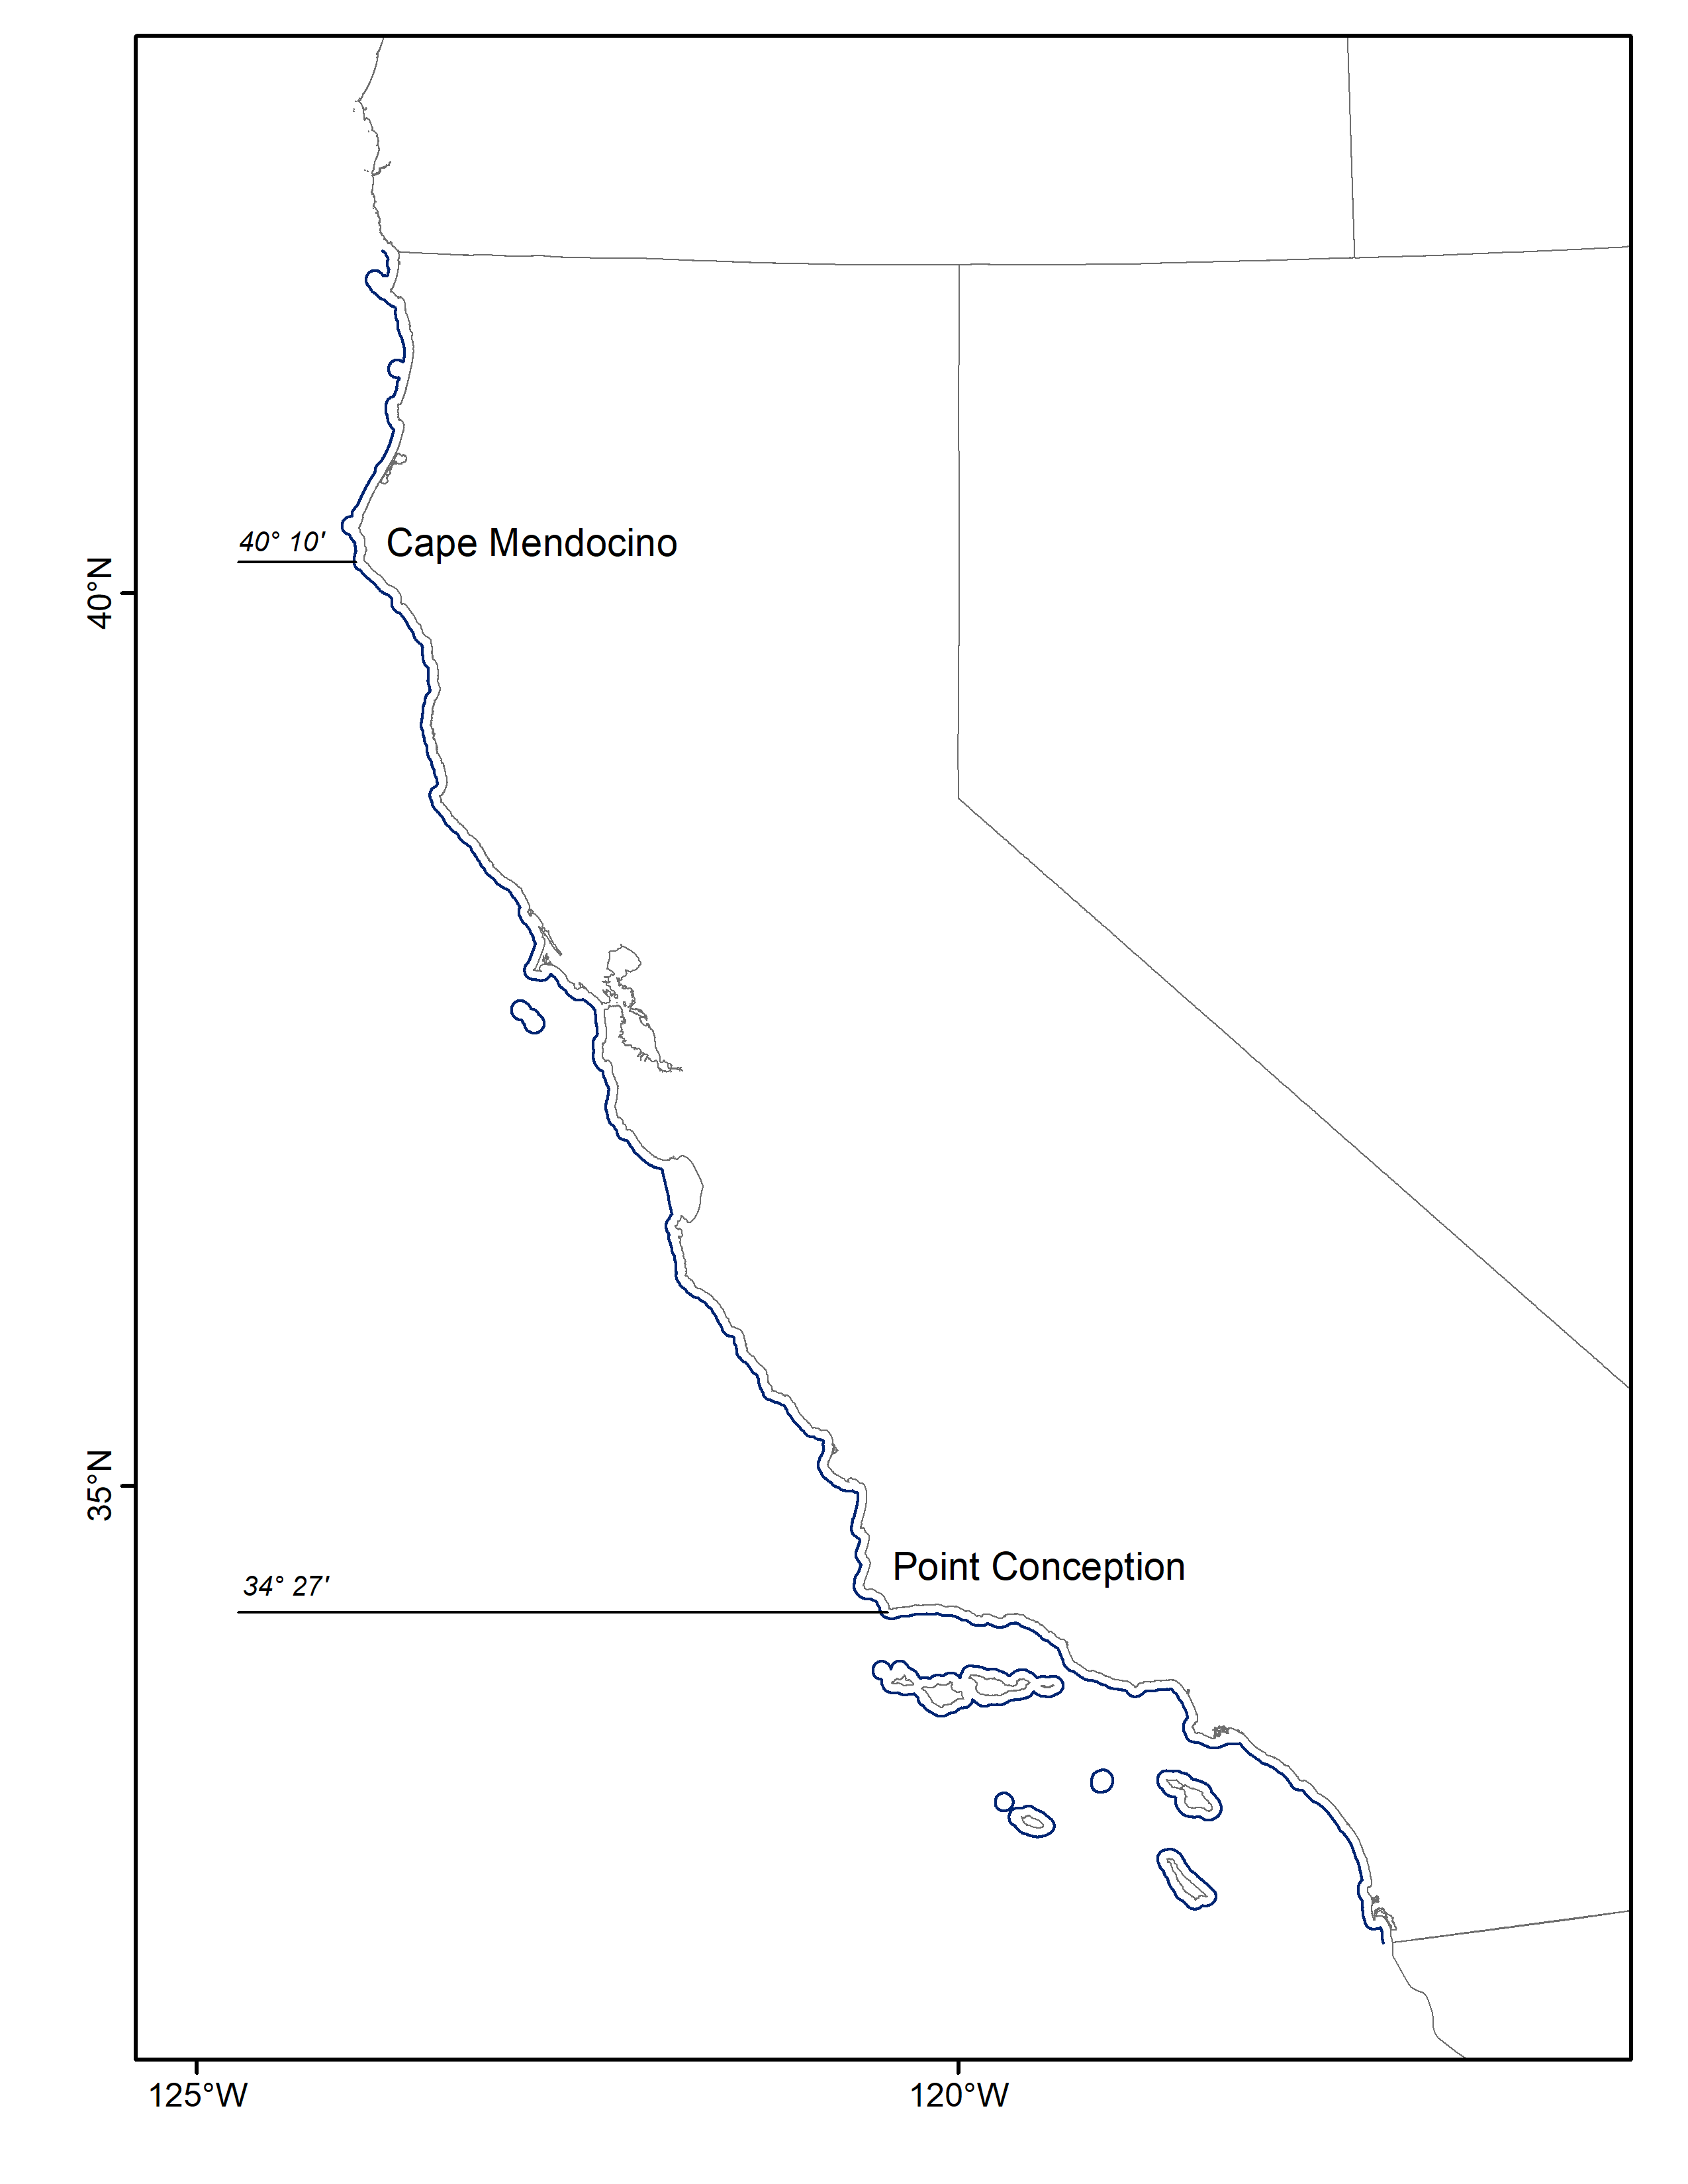
\includegraphics[width=1\textwidth,height=1\textheight]{C:/Stock_Assessments/VRML_Assessment_2021/GitHub/Vermilion_2021/doc/figures/assess_area.png}
\caption{Map of the assssment area with the 3 nm California state water boundary. The northern California model includes areas from Point Conception to the California-Oregon border and the southern California assessment includes areas from Point Concpetion to the USA-Mexico border.\label{fig:assess-area}}
\end{figure}

\begin{figure}
\centering
\includegraphics[width=1\textwidth,height=1\textheight]{C:/Stock_Assessments/VRML_Assessment_2021/Model_files/SCA/Verm21SoCA_089_pre-STAR_base_with_SS_OPT/plots/catch2 landings stacked.png}
\caption{Catches by fleet used in the base model.\label{fig:catch}}
\end{figure}

\begin{figure}
\centering
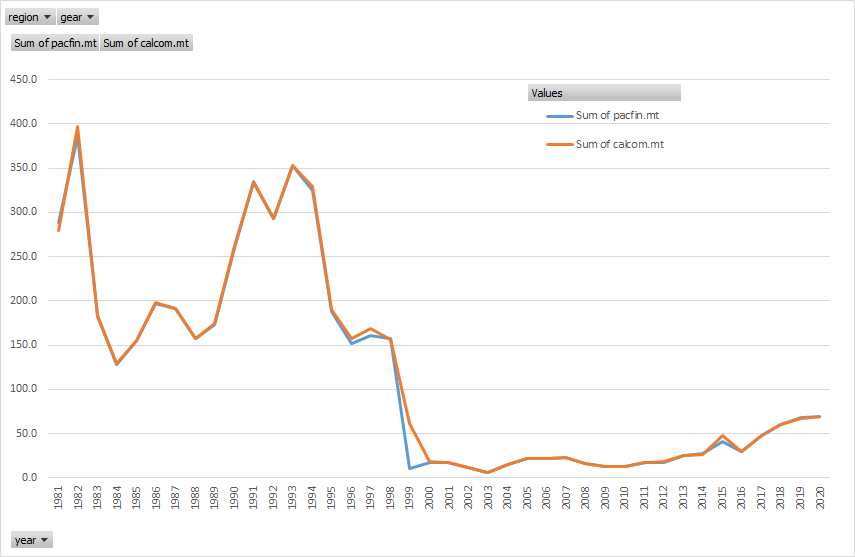
\includegraphics[width=1\textwidth,height=1\textheight]{C:/Stock_Assessments/VRML_Assessment_2021/GitHub/Vermilion_2021/doc/figures/compare_pacfin_calcom.png}
\caption{Comparison of landings from CALCOM and PacFIN.\label{fig:calcom-pacfin}}
\end{figure}

\begin{figure}
\centering
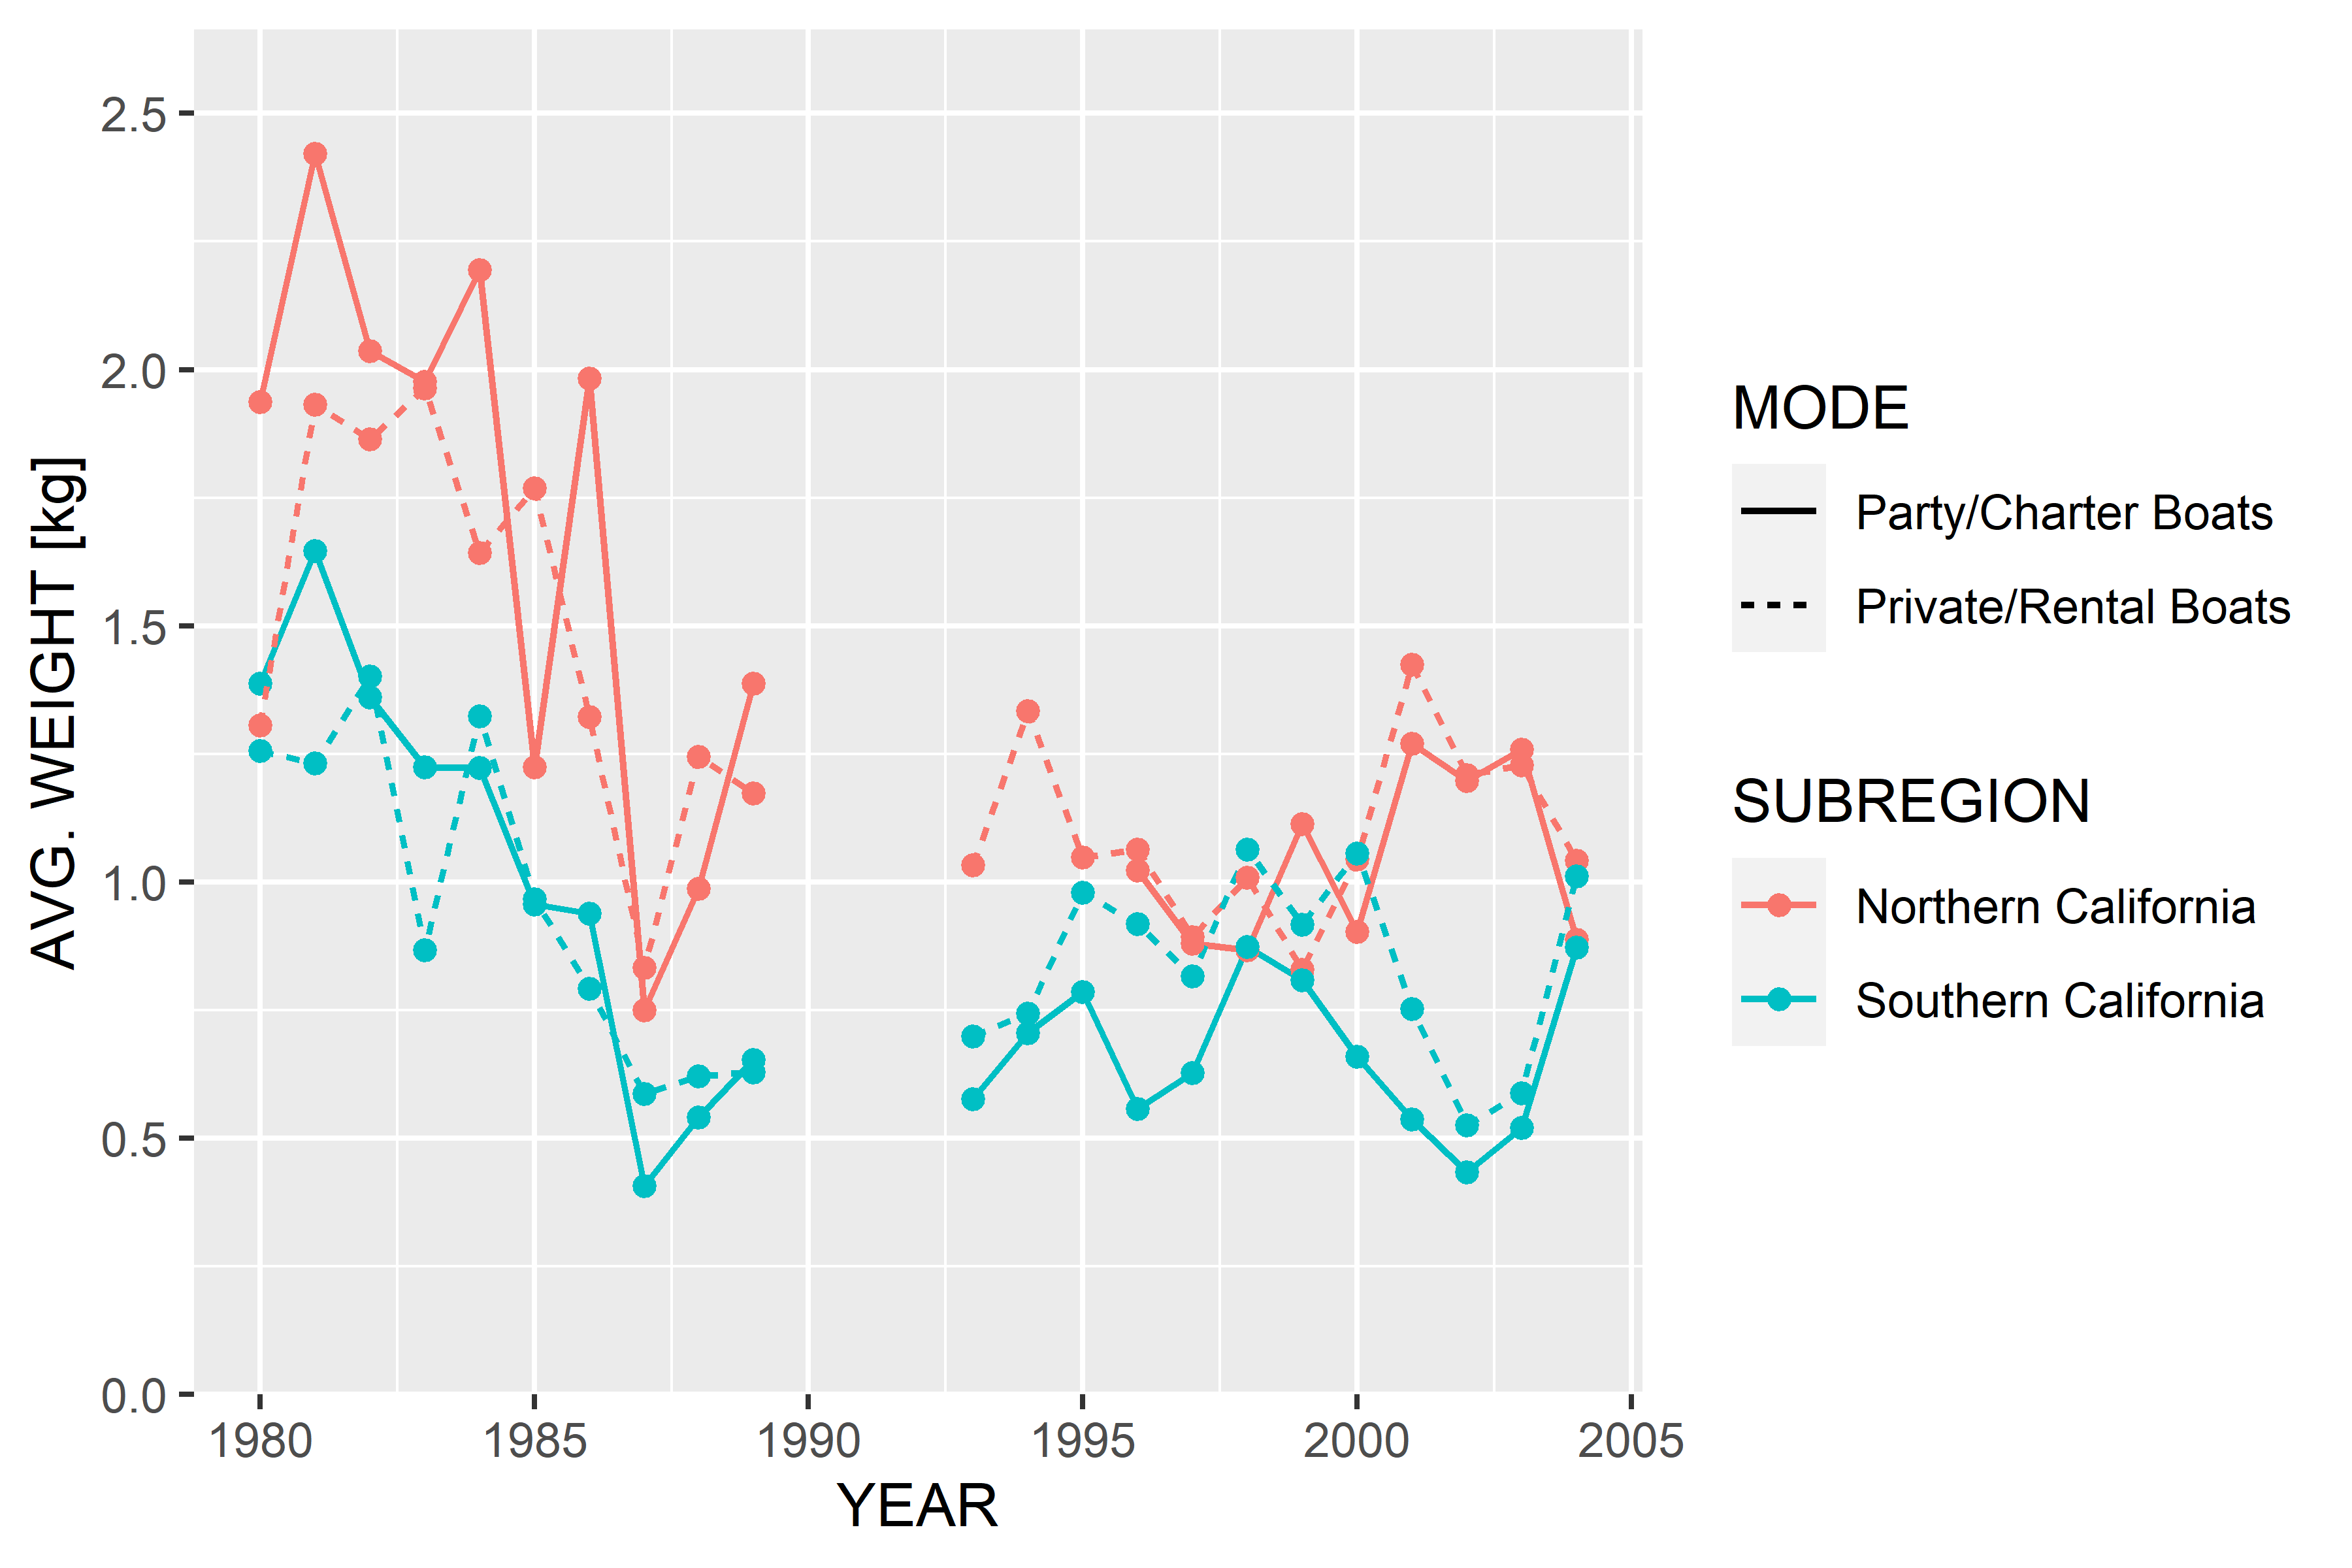
\includegraphics[width=1\textwidth,height=1\textheight]{C:/Stock_Assessments/VRML_Assessment_2021/GitHub/Vermilion_2021/doc/figures/rec_avg_weight.png}
\caption{Average weights calculated from the recreational landings data on RecFIN.\label{fig:rec-avg-weights}}
\end{figure}

\begin{figure}
\centering
\includegraphics[width=1\textwidth,height=1\textheight]{C:/Stock_Assessments/VRML_Assessment_2021/Model_files/SCA/Verm21SoCA_089_pre-STAR_base_with_SS_OPT/plots/comp_lendat_bubflt1mkt0_page2.png}
\caption{Length composition data from the commercial hook-and-line fishery.\label{fig:len-data-COM-HKL}}
\end{figure}

\begin{figure}
\centering
\includegraphics[width=1\textwidth,height=1\textheight]{C:/Stock_Assessments/VRML_Assessment_2021/Model_files/SCA/Verm21SoCA_089_pre-STAR_base_with_SS_OPT/plots/comp_lendat_bubflt3mkt0.png}
\caption{Length composition data from the commercial net fishery.\label{fig:len-data-COM-NET}}
\end{figure}

\begin{figure}
\centering
\includegraphics[width=1\textwidth,height=1\textheight]{C:/Stock_Assessments/VRML_Assessment_2021/Model_files/SCA/Verm21SoCA_089_pre-STAR_base_with_SS_OPT/plots/comp_lendat_bubflt4mkt0_page2.png}
\caption{Length composition data from the recreational PC retained fishery.\label{fig:len-data-REC-PC}}
\end{figure}

\begin{figure}
\centering
\includegraphics[width=1\textwidth,height=1\textheight]{C:/Stock_Assessments/VRML_Assessment_2021/Model_files/SCA/Verm21SoCA_089_pre-STAR_base_with_SS_OPT/plots/comp_lendat_bubflt5mkt0.png}
\caption{Length composition data from the recreational PC discard fishery.\label{fig:len-data-REC-PC-DIS}}
\end{figure}

\begin{figure}
\centering
\includegraphics[width=1\textwidth,height=1\textheight]{C:/Stock_Assessments/VRML_Assessment_2021/Model_files/SCA/Verm21SoCA_089_pre-STAR_base_with_SS_OPT/plots/comp_lendat_bubflt6mkt0_page2.png}
\caption{Length composition data from the recreational PR retained fishery.\label{fig:len-data-REC-PR}}
\end{figure}

\begin{figure}
\centering
\includegraphics[width=1\textwidth,height=1\textheight]{C:/Stock_Assessments/VRML_Assessment_2021/Model_files/SCA/Verm21SoCA_089_pre-STAR_base_with_SS_OPT/plots/comp_lendat_bubflt8mkt0.png}
\caption{Length composition data from the NWFSC hook-and-line survey.\label{fig:len-data-NWFSC-HKL}}
\end{figure}

\begin{figure}
\centering
\includegraphics[width=1\textwidth,height=1\textheight]{C:/Stock_Assessments/VRML_Assessment_2021/Model_files/SCA/Verm21SoCA_089_pre-STAR_base_with_SS_OPT/plots/comp_lendat_bubflt9mkt0.png}
\caption{Length composition data from the West Coast Groundfish Bottomfish Trawl Survey.\label{fig:len-data-NWFSC-TWL}}
\end{figure}

\begin{figure}
\centering
\includegraphics[width=1\textwidth,height=1\textheight]{C:/Stock_Assessments/VRML_Assessment_2021/Model_files/SCA/Verm21SoCA_089_pre-STAR_base_with_SS_OPT/plots/comp_lendat_bubflt11mkt0.png}
\caption{Length composition data from the CDFW reserach (aka green binder) survey.\label{fig:len-data-CDFW-RESEARCH}}
\end{figure}

\begin{figure}
\centering
\includegraphics[width=1\textwidth,height=1\textheight]{C:/Stock_Assessments/VRML_Assessment_2021/Model_files/SCA/Verm21SoCA_089_pre-STAR_base_with_SS_OPT/plots/comp_lendat_bubflt12mkt0.png}
\caption{Length composition data from the Early years hook-and-line.\label{fig:len-data-EARLY-HKL}}
\end{figure}

\begin{figure}
\centering
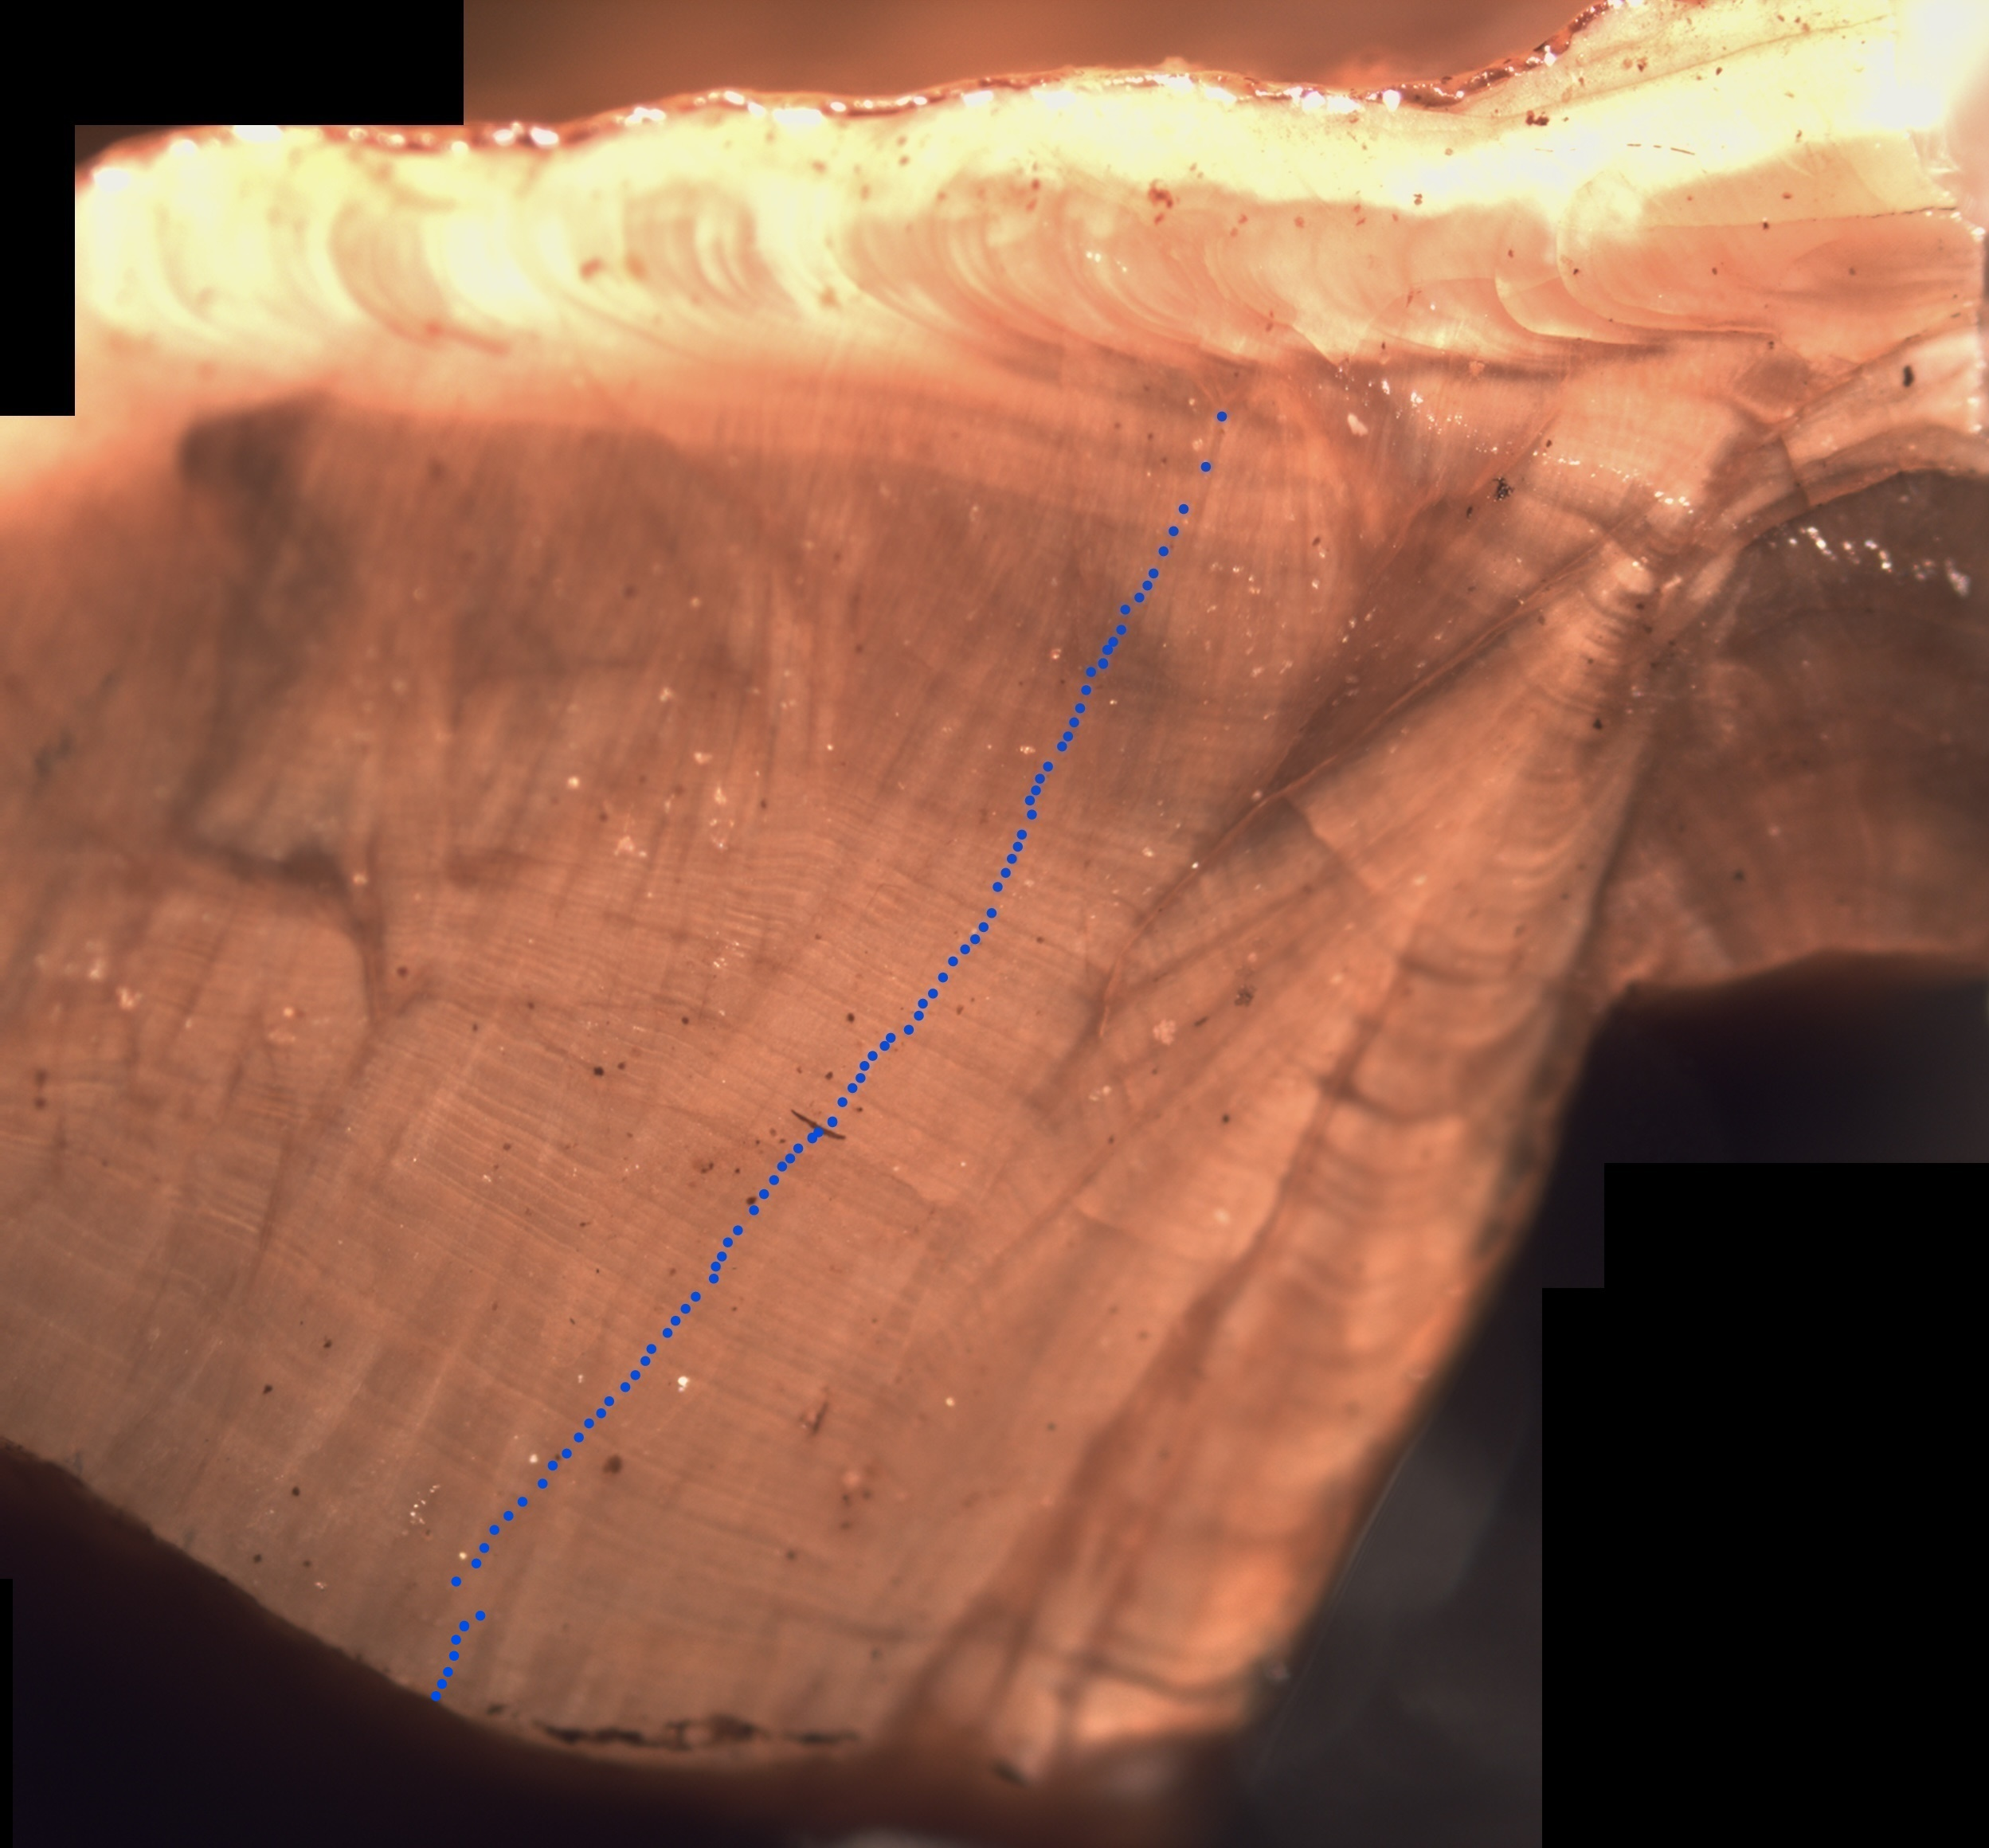
\includegraphics[width=1\textwidth,height=1\textheight]{C:/Stock_Assessments/VRML_Assessment_2021/GitHub/Vermilion_2021/doc/figures/oldfish.jpg}
\caption{Photograph of the \emph{oldest} aged fish used in the assessment with annuli marked by B. Kamikawa (NWFSC).\label{fig:oldfish}}
\end{figure}

\begin{figure}
\centering
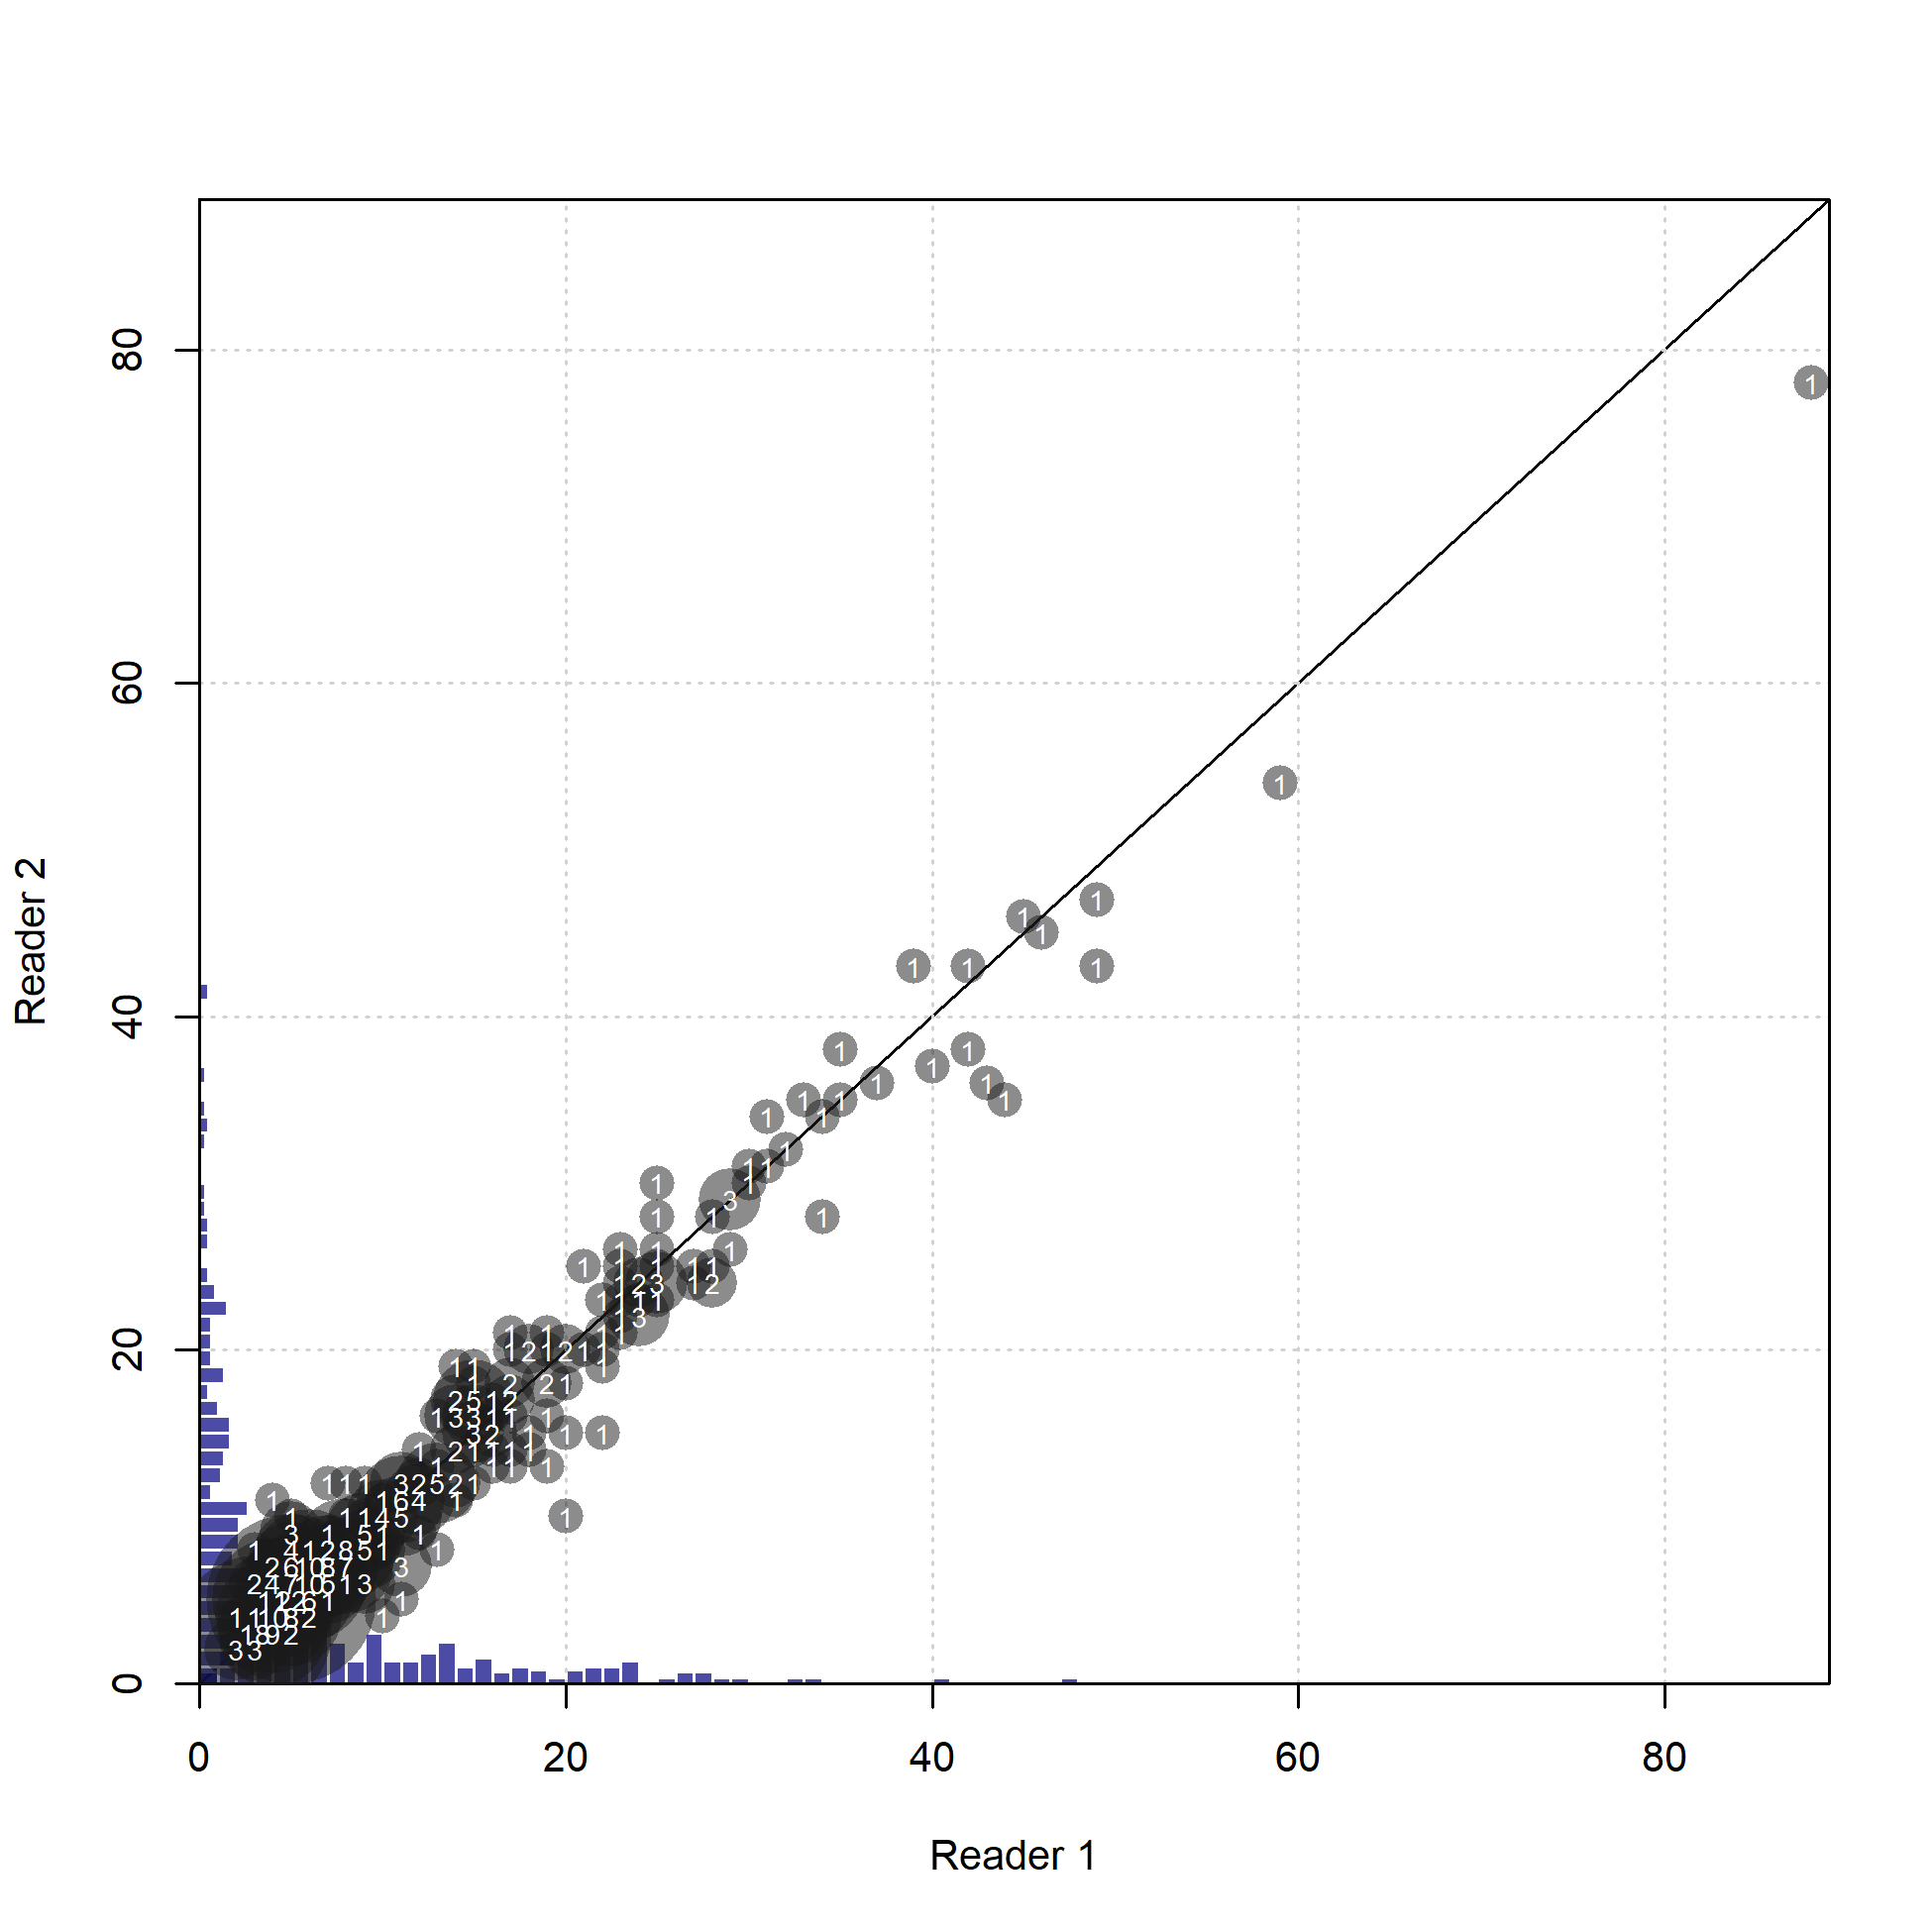
\includegraphics[width=1\textwidth,height=1\textheight]{C:/Stock_Assessments/VRML_Assessment_2021/GitHub/Vermilion_2021/doc/figures/Reader 1 vs Reader 2.png}
\caption{Aging precision between initial and blind double reads for vermilion.
Numbers in the bubbles are the sample sizes of otoliths cross-read.\label{fig:reader1reader2}}
\end{figure}

\begin{figure}
\centering
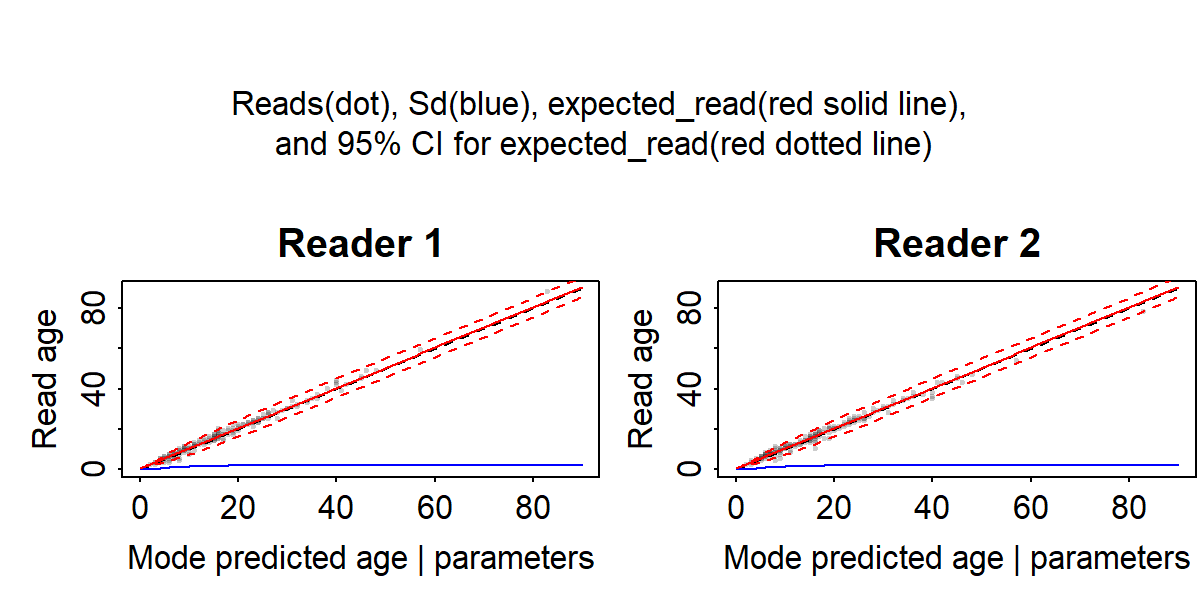
\includegraphics[width=1\textwidth,height=1\textheight]{C:/Stock_Assessments/VRML_Assessment_2021/GitHub/Vermilion_2021/doc/figures/True vs Reads (by reader).png}
\caption{True versus predicted age for two current age readers at the NWFSC
from the ageing error software with unbiased reads for reader 1 and curvilinear
bias for reader 1 and curvilinear standard deviation for both readers.\label{fig:truereads}}
\end{figure}

\begin{figure}
\centering
\includegraphics[width=1\textwidth,height=1\textheight]{C:/Stock_Assessments/VRML_Assessment_2021/Model_files/SCA/Verm21SoCA_089_pre-STAR_base_with_SS_OPT//plots/numbers10_ageerror_matrix_1.png}
\caption{Distribution of observed age at true age for ageing error type 1.\label{fig:ageerror}}
\end{figure}

\begin{figure}
\centering
\includegraphics[width=1\textwidth,height=1\textheight]{C:/Stock_Assessments/VRML_Assessment_2021/Model_files/SCA/Verm21SoCA_089_pre-STAR_base_with_SS_OPT//plots/bio5_weightatsize.png}
\caption{Weight-length relationship.\label{fig:weightlength}}
\end{figure}

\begin{figure}
\centering
\includegraphics[width=1\textwidth,height=1\textheight]{C:/Stock_Assessments/VRML_Assessment_2021/Model_files/SCA/Verm21SoCA_089_pre-STAR_base_with_SS_OPT//plots/bio6_maturity.png}
\caption{Maturity at length.\label{fig:maturity}}
\end{figure}

\begin{figure}
\centering
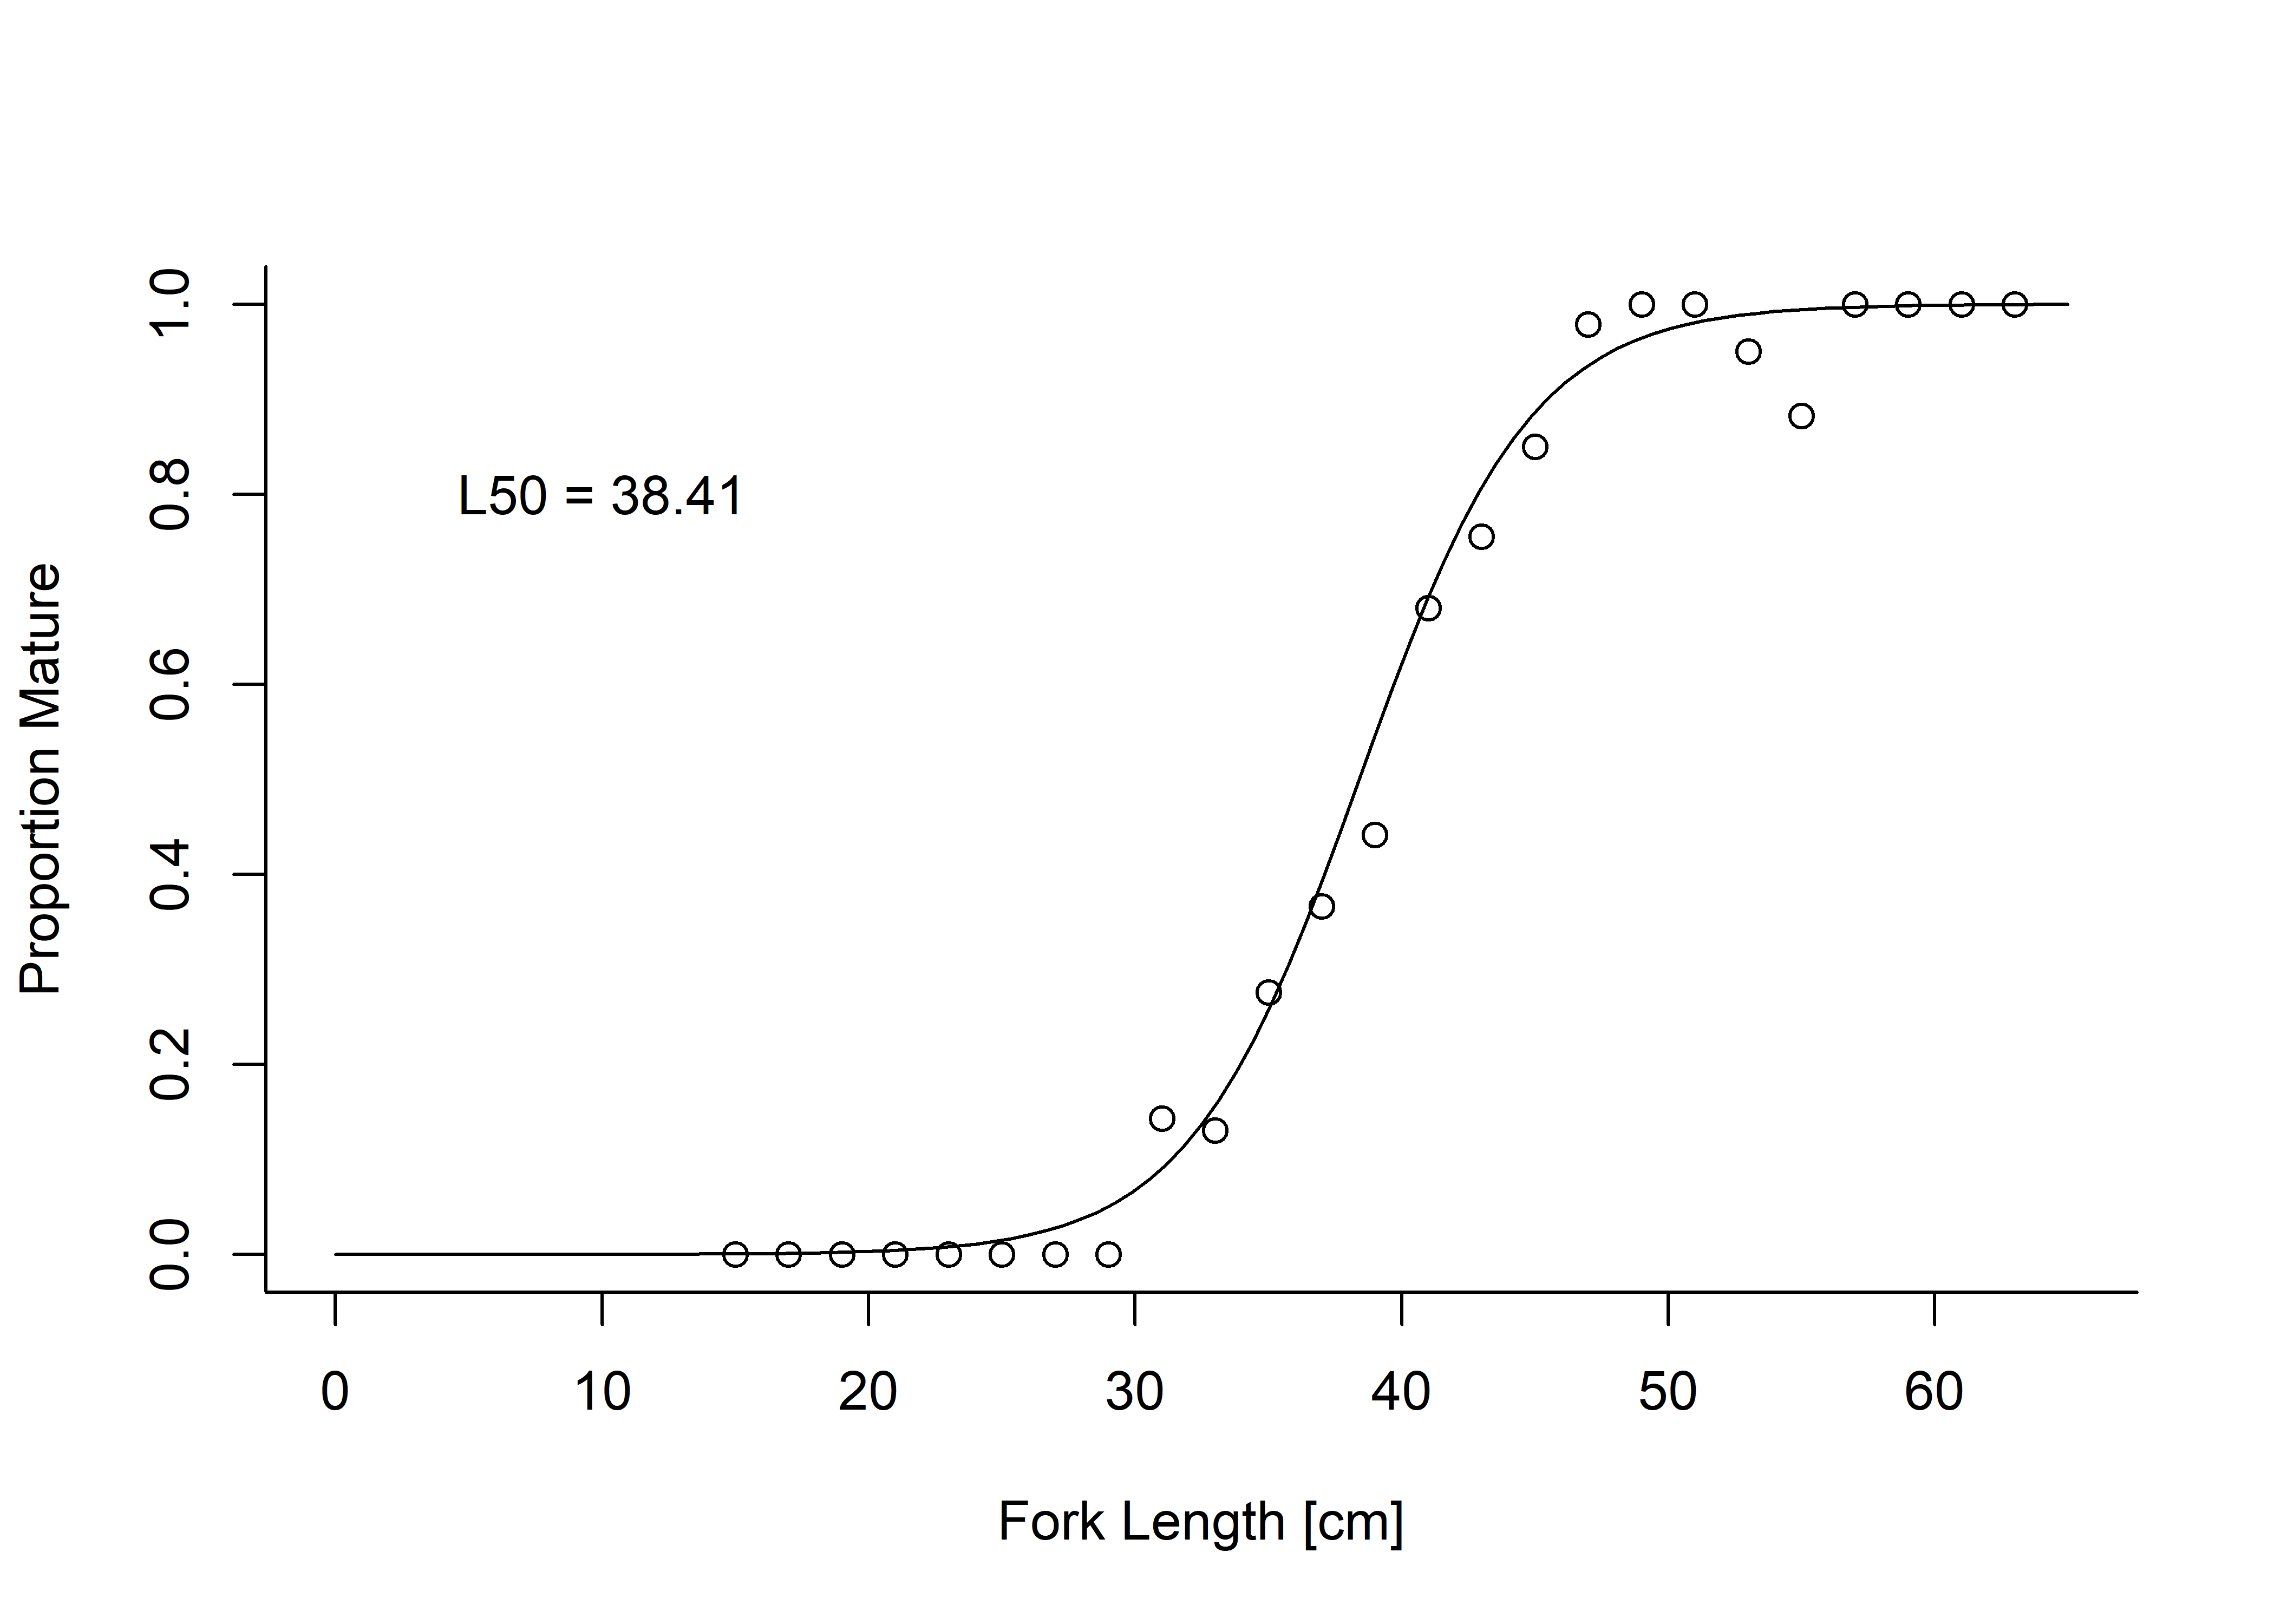
\includegraphics[width=1\textwidth,height=1\textheight]{C:/Stock_Assessments/VRML_Assessment_2021/GitHub/Vermilion_2021/doc/figures/vermilion_functional_maturity.png}
\caption{Fitted logistic regression of estimated functional maturity as a function of fork length for vermilion rockfish.\label{fig:functional-maturity}}
\end{figure}

\begin{figure}
\centering
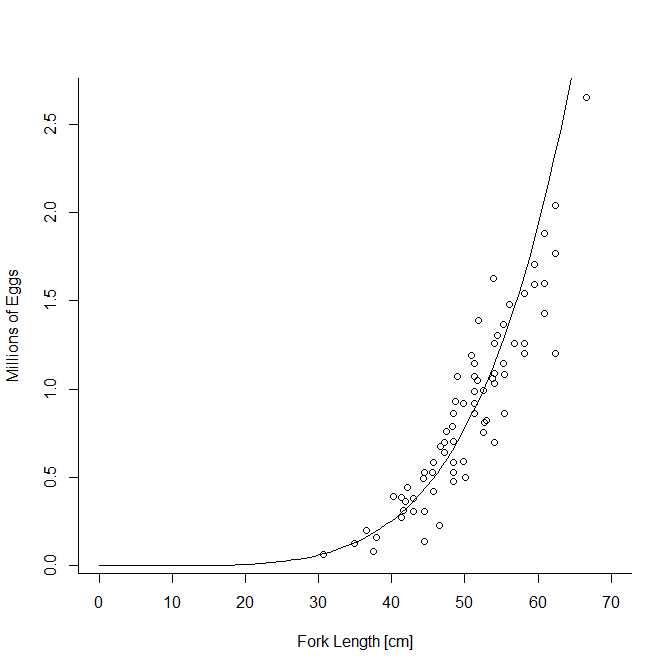
\includegraphics[width=1\textwidth,height=1\textheight]{C:/Stock_Assessments/VRML_Assessment_2021/GitHub/Vermilion_2021/doc/figures/fitted_fec_len.png}
\caption{Fitted fecundity as a function of weight from samples of vermilion rockfish.\label{fig:fitted-fecundity}}
\end{figure}

\begin{figure}
\centering
\includegraphics[width=1\textwidth,height=1\textheight]{C:/Stock_Assessments/VRML_Assessment_2021/Model_files/SCA/Verm21SoCA_089_pre-STAR_base_with_SS_OPT//plots/bio8_fecundity_wt.png}
\caption{Fecundity as a function of weight.\label{fig:fecundity}}
\end{figure}

\begin{figure}
\centering
\includegraphics[width=1\textwidth,height=1\textheight]{C:/Stock_Assessments/VRML_Assessment_2021/Model_files/SCA/Verm21SoCA_089_pre-STAR_base_with_SS_OPT/plots/bio11_spawningoutput_age.png}
\caption{Spawning output at age. This is the product of maturity and fecundity. When these processes are length-based they are converted into the age dimension using the matrix of length at age.\label{fig:spawnage}}
\end{figure}

\FloatBarrier

\begin{figure}
\centering
\includegraphics[width=1\textwidth,height=1\textheight]{C:/Stock_Assessments/VRML_Assessment_2021/Model_files/SCA/Verm21SoCA_089_pre-STAR_base_with_SS_OPT//plots/sexratio_len_flt11mkt0.png}
\caption{Sex ratios for length comps, whole catch, CDFW reserach (aka green binder) survey. Observed sex ratios (points) with 75\% intervals (vertical lines) calculated as a Jeffreys interval based on the adjusted input sample size. The model expectation is shown in the purple line.\label{fig:sexratio-CDFW-RESEARCH}}
\end{figure}

\begin{figure}
\centering
\includegraphics[width=1\textwidth,height=1\textheight]{C:/Stock_Assessments/VRML_Assessment_2021/Model_files/SCA/Verm21SoCA_089_pre-STAR_base_with_SS_OPT//plots/sexratio_len_flt12mkt0.png}
\caption{Sex ratios for length comps, whole catch, Early years hook-and-line. Observed sex ratios (points) with 75\% intervals (vertical lines) calculated as a Jeffreys interval based on the adjusted input sample size. The model expectation is shown in the purple line.\label{fig:sexratio-EARLY-HKL}}
\end{figure}

\begin{figure}
\centering
\includegraphics[width=1\textwidth,height=1\textheight]{C:/Stock_Assessments/VRML_Assessment_2021/Model_files/SCA/Verm21SoCA_089_pre-STAR_base_with_SS_OPT//plots/sexratio_len_flt8mkt0.png}
\caption{Sex ratios for length comps, whole catch, NWFSC hook-and-line survey. Observed sex ratios (points) with 75\% intervals (vertical lines) calculated as a Jeffreys interval based on the adjusted input sample size. The model expectation is shown in the purple line.\label{fig:sexratio-NWFSC-HKL}}
\end{figure}

\begin{figure}
\centering
\includegraphics[width=1\textwidth,height=1\textheight]{C:/Stock_Assessments/VRML_Assessment_2021/Model_files/SCA/Verm21SoCA_089_pre-STAR_base_with_SS_OPT//plots/sexratio_len_flt9mkt0.png}
\caption{Sex ratios for length comps, whole catch, West Coast Groundfish Bottomfish Trawl Survey. Observed sex ratios (points) with 75\% intervals (vertical lines) calculated as a Jeffreys interval based on the adjusted input sample size. The model expectation is shown in the purple line.\label{fig:sexratio-NWFSC-TWL}}
\end{figure}

\FloatBarrier

\begin{figure}
\centering
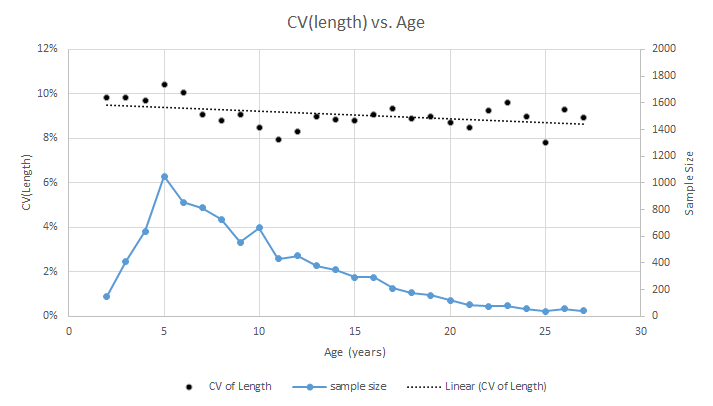
\includegraphics[width=1\textwidth,height=1\textheight]{C:/Stock_Assessments/VRML_Assessment_2021/GitHub/Vermilion_2021/doc/figures/CV_of_Length_vs_Age.png}
\caption{Coefficient of variation of length versus age for vermilion rockfish from the NWFSC hook-and-line survey.\label{fig:cv-length-age}}
\end{figure}

\begin{figure}
\centering
\includegraphics[width=1\textwidth,height=1\textheight]{C:/Stock_Assessments/VRML_Assessment_2021/GitHub/Vermilion_2021/doc/figures/jitter_preSTAR_base_SCA.png}
\caption{Results from 100 jittered runs of the pre-STAR base model.\label{fig:jitter}}
\end{figure}

\begin{figure}
\centering
\includegraphics[width=1\textwidth,height=1\textheight]{C:/Stock_Assessments/VRML_Assessment_2021/Model_files/SCA/Verm21SoCA_089_pre-STAR_base_with_SS_OPT//plots/bio1_sizeatage.png}
\caption{Length at age in the beginning of the year (or season) in the ending year of the model. Shaded area indicates 95\% distribution of length at age around estimated growth curve.\label{fig:fittedgrowth}}
\end{figure}

\FloatBarrier

\begin{figure}
\centering
\includegraphics[width=1\textwidth,height=1\textheight]{C:/Stock_Assessments/VRML_Assessment_2021/Model_files/SCA/Verm21SoCA_089_pre-STAR_base_with_SS_OPT//plots/sel01_multiple_fleets_length1.png}
\caption{End year selectivity at length by fleet/survey.\label{fig:selex-length-all}}
\end{figure}

\FloatBarrier

\begin{figure}
\centering
\includegraphics[width=1\textwidth,height=1\textheight]{C:/Stock_Assessments/VRML_Assessment_2021/Model_files/SCA/Verm21SoCA_089_pre-STAR_base_with_SS_OPT//plots/sel02_multiple_fleets_age2.png}
\caption{Selectivity at age derived from selectivity at length for multiple fleets.\label{fig:selex-age-all}}
\end{figure}

\begin{figure}
\centering
\includegraphics[width=1\textwidth,height=1\textheight]{C:/Stock_Assessments/VRML_Assessment_2021/Model_files/SCA/Verm21SoCA_089_pre-STAR_base_with_SS_OPT//plots/sel03_len_timevary_surf_flt1sex1.png}
\caption{Surface plot of Female time-varying selectivity for COM\_HKL.\label{fig:sel03_len_timevary_surf_flt1sex1}}
\end{figure}

\begin{figure}
\centering
\includegraphics[width=1\textwidth,height=1\textheight]{C:/Stock_Assessments/VRML_Assessment_2021/Model_files/SCA/Verm21SoCA_089_pre-STAR_base_with_SS_OPT//plots/sel03_len_timevary_surf_flt2sex1.png}
\caption{Surface plot of Female time-varying selectivity for COM\_TWL.\label{fig:sel03_len_timevary_surf_flt2sex1}}
\end{figure}

\begin{figure}
\centering
\includegraphics[width=1\textwidth,height=1\textheight]{C:/Stock_Assessments/VRML_Assessment_2021/Model_files/SCA/Verm21SoCA_089_pre-STAR_base_with_SS_OPT//plots/sel03_len_timevary_surf_flt4sex1.png}
\caption{Surface plot of Female time-varying selectivity for REC\_PC.\label{fig:sel03_len_timevary_surf_flt4sex1}}
\end{figure}

\begin{figure}
\centering
\includegraphics[width=1\textwidth,height=1\textheight]{C:/Stock_Assessments/VRML_Assessment_2021/Model_files/SCA/Verm21SoCA_089_pre-STAR_base_with_SS_OPT//plots/sel03_len_timevary_surf_flt6sex1.png}
\caption{Surface plot of Female time-varying selectivity for REC\_PR.\label{fig:sel03_len_timevary_surf_flt6sex1}}
\end{figure}

\FloatBarrier

\FloatBarrier

\begin{figure}
\centering
\includegraphics[width=1\textwidth,height=1\textheight]{C:/Stock_Assessments/VRML_Assessment_2021/Model_files/SCA/Verm21SoCA_089_pre-STAR_base_with_SS_OPT//plots/sel09_len_flt1sex1.png}
\caption{Female ending year selectivity for the commercial hook-and-line fishery.\label{fig:endyr-selex-COM-HKL}}
\end{figure}

\begin{figure}
\centering
\includegraphics[width=1\textwidth,height=1\textheight]{C:/Stock_Assessments/VRML_Assessment_2021/Model_files/SCA/Verm21SoCA_089_pre-STAR_base_with_SS_OPT//plots/sel09_len_flt3sex1.png}
\caption{Female ending year selectivity for the commercial net fishery.\label{fig:endyr-selex-COM-NET}}
\end{figure}

\begin{figure}
\centering
\includegraphics[width=1\textwidth,height=1\textheight]{C:/Stock_Assessments/VRML_Assessment_2021/Model_files/SCA/Verm21SoCA_089_pre-STAR_base_with_SS_OPT//plots/sel09_len_flt4sex1.png}
\caption{Female ending year selectivity for the recreational PC retained fishery.\label{fig:endyr-selex-REC-PC}}
\end{figure}

\begin{figure}
\centering
\includegraphics[width=1\textwidth,height=1\textheight]{C:/Stock_Assessments/VRML_Assessment_2021/Model_files/SCA/Verm21SoCA_089_pre-STAR_base_with_SS_OPT//plots/sel09_len_flt5sex1.png}
\caption{Female ending year selectivity for the recreational PC discard fishery.\label{fig:endyr-selex-REC-PC-DIS}}
\end{figure}

\begin{figure}
\centering
\includegraphics[width=1\textwidth,height=1\textheight]{C:/Stock_Assessments/VRML_Assessment_2021/Model_files/SCA/Verm21SoCA_089_pre-STAR_base_with_SS_OPT//plots/sel09_len_flt6sex1.png}
\caption{Female ending year selectivity for the recreational PR retained fishery.\label{fig:endyr-selex-REC-PR}}
\end{figure}

\begin{figure}
\centering
\includegraphics[width=1\textwidth,height=1\textheight]{C:/Stock_Assessments/VRML_Assessment_2021/Model_files/SCA/Verm21SoCA_089_pre-STAR_base_with_SS_OPT//plots/sel09_len_flt8sex1.png}
\caption{Female ending year selectivity for the NWFSC hook-and-line survey.\label{fig:endyr-selex-NWFSC-HKL}}
\end{figure}

\begin{figure}
\centering
\includegraphics[width=1\textwidth,height=1\textheight]{C:/Stock_Assessments/VRML_Assessment_2021/Model_files/SCA/Verm21SoCA_089_pre-STAR_base_with_SS_OPT//plots/sel09_len_flt9sex1.png}
\caption{Female ending year selectivity for the West Coast Groundfish Bottomfish Trawl Survey.\label{fig:endyr-selex-NWFSC-TWL}}
\end{figure}

\begin{figure}
\centering
\includegraphics[width=1\textwidth,height=1\textheight]{C:/Stock_Assessments/VRML_Assessment_2021/Model_files/SCA/Verm21SoCA_089_pre-STAR_base_with_SS_OPT//plots/sel09_len_flt11sex1.png}
\caption{Female ending year selectivity for the CDFW reserach (aka green binder) survey.\label{fig:endyr-selex-CDFW-RESEARCH}}
\end{figure}

\begin{figure}
\centering
\includegraphics[width=1\textwidth,height=1\textheight]{C:/Stock_Assessments/VRML_Assessment_2021/Model_files/SCA/Verm21SoCA_089_pre-STAR_base_with_SS_OPT//plots/sel09_len_flt12sex1.png}
\caption{Female ending year selectivity for the Early years hook-and-line.\label{fig:endyr-selex-EARLY-HKL}}
\end{figure}

\FloatBarrier

\clearpage
\FloatBarrier

\FloatBarrier

\begin{figure}
\centering
\includegraphics[width=1\textwidth,height=1\textheight]{C:/Stock_Assessments/VRML_Assessment_2021/Model_files/SCA/Verm21SoCA_089_pre-STAR_base_with_SS_OPT//plots/comp_lenfit__aggregated_across_time.png}
\caption{Length comps, aggregated across time by fleet.
Labels `retained' and `discard' indicate discarded or retained sampled for each fleet. Panels without this designation represent the whole catch.\label{fig:lenfits-all}}
\end{figure}

\FloatBarrier

\begin{figure}
\centering
\includegraphics[width=1\textwidth,height=1\textheight]{C:/Stock_Assessments/VRML_Assessment_2021/Model_files/SCA/Verm21SoCA_089_pre-STAR_base_with_SS_OPT//plots/comp_lenfit_residsflt1mkt0_page2.png}
\caption{Pearson residuals for the commercial hook-and-line fishery. Closed bubbles are positive residuals (observed \textgreater{} expected) and open bubbles are negative residuals (observed \textless{} expected).\label{fig:len-pearson-COM-HKL}}
\end{figure}

\begin{figure}
\centering
\includegraphics[width=1\textwidth,height=1\textheight]{C:/Stock_Assessments/VRML_Assessment_2021/Model_files/SCA/Verm21SoCA_089_pre-STAR_base_with_SS_OPT//plots/comp_lenfit_data_weighting_TA1.8_COM_HKL.png}
\caption{Mean length for REC\_PR with 95\% confidence intervals based on current samples sizes. Francis data weighting method TA1.8: thinner intervals (with capped ends) show result of further adjusting sample sizes based on suggested multiplier (with 95\% interval) for length data from the commercial hook-and-line fishery.\label{fig:mean-len-fit-COM-HKL}}
\end{figure}

\begin{figure}
\centering
\includegraphics[width=1\textwidth,height=1\textheight]{C:/Stock_Assessments/VRML_Assessment_2021/Model_files/SCA/Verm21SoCA_089_pre-STAR_base_with_SS_OPT//plots/comp_lenfit_residsflt3mkt0.png}
\caption{Pearson residuals for the commercial net fishery. Closed bubbles are positive residuals (observed \textgreater{} expected) and open bubbles are negative residuals (observed \textless{} expected).\label{fig:len-pearson-COM-NET}}
\end{figure}

\begin{figure}
\centering
\includegraphics[width=1\textwidth,height=1\textheight]{C:/Stock_Assessments/VRML_Assessment_2021/Model_files/SCA/Verm21SoCA_089_pre-STAR_base_with_SS_OPT//plots/comp_lenfit_data_weighting_TA1.8_COM_NET.png}
\caption{Mean length for REC\_PR with 95\% confidence intervals based on current samples sizes. Francis data weighting method TA1.8: thinner intervals (with capped ends) show result of further adjusting sample sizes based on suggested multiplier (with 95\% interval) for length data from the commercial net fishery.\label{fig:mean-len-fit-COM-NET}}
\end{figure}

\begin{figure}
\centering
\includegraphics[width=1\textwidth,height=1\textheight]{C:/Stock_Assessments/VRML_Assessment_2021/Model_files/SCA/Verm21SoCA_089_pre-STAR_base_with_SS_OPT//plots/comp_lenfit_residsflt4mkt0_page2.png}
\caption{Pearson residuals for the recreational PC retained fishery. Closed bubbles are positive residuals (observed \textgreater{} expected) and open bubbles are negative residuals (observed \textless{} expected).\label{fig:len-pearson-REC-PC}}
\end{figure}

\begin{figure}
\centering
\includegraphics[width=1\textwidth,height=1\textheight]{C:/Stock_Assessments/VRML_Assessment_2021/Model_files/SCA/Verm21SoCA_089_pre-STAR_base_with_SS_OPT//plots/comp_lenfit_data_weighting_TA1.8_REC_PC.png}
\caption{Mean length for REC\_PR with 95\% confidence intervals based on current samples sizes. Francis data weighting method TA1.8: thinner intervals (with capped ends) show result of further adjusting sample sizes based on suggested multiplier (with 95\% interval) for length data from the recreational PC retained fishery.\label{fig:mean-len-fit-REC-PC}}
\end{figure}

\begin{figure}
\centering
\includegraphics[width=1\textwidth,height=1\textheight]{C:/Stock_Assessments/VRML_Assessment_2021/Model_files/SCA/Verm21SoCA_089_pre-STAR_base_with_SS_OPT//plots/comp_lenfit_residsflt5mkt0.png}
\caption{Pearson residuals for the recreational PC discard fishery. Closed bubbles are positive residuals (observed \textgreater{} expected) and open bubbles are negative residuals (observed \textless{} expected).\label{fig:len-pearson-REC-PC-DIS}}
\end{figure}

\begin{figure}
\centering
\includegraphics[width=1\textwidth,height=1\textheight]{C:/Stock_Assessments/VRML_Assessment_2021/Model_files/SCA/Verm21SoCA_089_pre-STAR_base_with_SS_OPT//plots/comp_lenfit_data_weighting_TA1.8_REC_PC_DIS.png}
\caption{Mean length for REC\_PR with 95\% confidence intervals based on current samples sizes. Francis data weighting method TA1.8: thinner intervals (with capped ends) show result of further adjusting sample sizes based on suggested multiplier (with 95\% interval) for length data from the recreational PC discard fishery.\label{fig:mean-len-fit-REC-PC-DIS}}
\end{figure}

\begin{figure}
\centering
\includegraphics[width=1\textwidth,height=1\textheight]{C:/Stock_Assessments/VRML_Assessment_2021/Model_files/SCA/Verm21SoCA_089_pre-STAR_base_with_SS_OPT//plots/comp_lenfit_residsflt6mkt0_page2.png}
\caption{Pearson residuals for the recreational PR retained fishery. Closed bubbles are positive residuals (observed \textgreater{} expected) and open bubbles are negative residuals (observed \textless{} expected).\label{fig:len-pearson-REC-PR}}
\end{figure}

\begin{figure}
\centering
\includegraphics[width=1\textwidth,height=1\textheight]{C:/Stock_Assessments/VRML_Assessment_2021/Model_files/SCA/Verm21SoCA_089_pre-STAR_base_with_SS_OPT//plots/comp_lenfit_data_weighting_TA1.8_REC_PR.png}
\caption{Mean length for REC\_PR with 95\% confidence intervals based on current samples sizes. Francis data weighting method TA1.8: thinner intervals (with capped ends) show result of further adjusting sample sizes based on suggested multiplier (with 95\% interval) for length data from the recreational PR retained fishery.\label{fig:mean-len-fit-REC-PR}}
\end{figure}

\begin{figure}
\centering
\includegraphics[width=1\textwidth,height=1\textheight]{C:/Stock_Assessments/VRML_Assessment_2021/Model_files/SCA/Verm21SoCA_089_pre-STAR_base_with_SS_OPT//plots/comp_lenfit_residsflt8mkt0.png}
\caption{Pearson residuals for the NWFSC hook-and-line survey. Closed bubbles are positive residuals (observed \textgreater{} expected) and open bubbles are negative residuals (observed \textless{} expected).\label{fig:len-pearson-NWFSC-HKL}}
\end{figure}

\begin{figure}
\centering
\includegraphics[width=1\textwidth,height=1\textheight]{C:/Stock_Assessments/VRML_Assessment_2021/Model_files/SCA/Verm21SoCA_089_pre-STAR_base_with_SS_OPT//plots/comp_lenfit_data_weighting_TA1.8_NWFSC_HKL.png}
\caption{Mean length for REC\_PR with 95\% confidence intervals based on current samples sizes. Francis data weighting method TA1.8: thinner intervals (with capped ends) show result of further adjusting sample sizes based on suggested multiplier (with 95\% interval) for length data from the NWFSC hook-and-line survey.\label{fig:mean-len-fit-NWFSC-HKL}}
\end{figure}

\begin{figure}
\centering
\includegraphics[width=1\textwidth,height=1\textheight]{C:/Stock_Assessments/VRML_Assessment_2021/Model_files/SCA/Verm21SoCA_089_pre-STAR_base_with_SS_OPT//plots/comp_lenfit_residsflt9mkt0.png}
\caption{Pearson residuals for the West Coast Groundfish Bottomfish Trawl Survey. Closed bubbles are positive residuals (observed \textgreater{} expected) and open bubbles are negative residuals (observed \textless{} expected).\label{fig:len-pearson-NWFSC-TWL}}
\end{figure}

\begin{figure}
\centering
\includegraphics[width=1\textwidth,height=1\textheight]{C:/Stock_Assessments/VRML_Assessment_2021/Model_files/SCA/Verm21SoCA_089_pre-STAR_base_with_SS_OPT//plots/comp_lenfit_data_weighting_TA1.8_NWFSC_TWL.png}
\caption{Mean length for REC\_PR with 95\% confidence intervals based on current samples sizes. Francis data weighting method TA1.8: thinner intervals (with capped ends) show result of further adjusting sample sizes based on suggested multiplier (with 95\% interval) for length data from the West Coast Groundfish Bottomfish Trawl Survey.\label{fig:mean-len-fit-NWFSC-TWL}}
\end{figure}

\begin{figure}
\centering
\includegraphics[width=1\textwidth,height=1\textheight]{C:/Stock_Assessments/VRML_Assessment_2021/Model_files/SCA/Verm21SoCA_089_pre-STAR_base_with_SS_OPT//plots/comp_lenfit_residsflt11mkt0.png}
\caption{Pearson residuals for the CDFW reserach (aka green binder) survey. Closed bubbles are positive residuals (observed \textgreater{} expected) and open bubbles are negative residuals (observed \textless{} expected).\label{fig:len-pearson-CDFW-RESEARCH}}
\end{figure}

\begin{figure}
\centering
\includegraphics[width=1\textwidth,height=1\textheight]{C:/Stock_Assessments/VRML_Assessment_2021/Model_files/SCA/Verm21SoCA_089_pre-STAR_base_with_SS_OPT//plots/comp_lenfit_data_weighting_TA1.8_CDFW_RESEARCH.png}
\caption{Mean length for REC\_PR with 95\% confidence intervals based on current samples sizes. Francis data weighting method TA1.8: thinner intervals (with capped ends) show result of further adjusting sample sizes based on suggested multiplier (with 95\% interval) for length data from the CDFW reserach (aka green binder) survey.\label{fig:mean-len-fit-CDFW-RESEARCH}}
\end{figure}

\begin{figure}
\centering
\includegraphics[width=1\textwidth,height=1\textheight]{C:/Stock_Assessments/VRML_Assessment_2021/Model_files/SCA/Verm21SoCA_089_pre-STAR_base_with_SS_OPT//plots/comp_lenfit_residsflt12mkt0.png}
\caption{Pearson residuals for the Early years hook-and-line. Closed bubbles are positive residuals (observed \textgreater{} expected) and open bubbles are negative residuals (observed \textless{} expected).\label{fig:len-pearson-EARLY-HKL}}
\end{figure}

\begin{figure}
\centering
\includegraphics[width=1\textwidth,height=1\textheight]{C:/Stock_Assessments/VRML_Assessment_2021/Model_files/SCA/Verm21SoCA_089_pre-STAR_base_with_SS_OPT//plots/comp_lenfit_data_weighting_TA1.8_EARLY_HKL.png}
\caption{Mean length for REC\_PR with 95\% confidence intervals based on current samples sizes. Francis data weighting method TA1.8: thinner intervals (with capped ends) show result of further adjusting sample sizes based on suggested multiplier (with 95\% interval) for length data from the Early years hook-and-line.\label{fig:mean-len-fit-EARLY-HKL}}
\end{figure}

\FloatBarrier

\FloatBarrier

\begin{figure}
\centering
\includegraphics[width=1\textwidth,height=1\textheight]{C:/Stock_Assessments/VRML_Assessment_2021/Model_files/SCA/Verm21SoCA_089_pre-STAR_base_with_SS_OPT//plots/index9_standcpueall.png}
\caption{Standardized indices overlaid. Each index is rescaled to have mean observation = 1.0.\label{fig:cpueall}}
\end{figure}

\begin{figure}
\centering
\includegraphics[width=1\textwidth,height=1\textheight]{C:/Stock_Assessments/VRML_Assessment_2021/Model_files/SCA/Verm21SoCA_089_pre-STAR_base_with_SS_OPT//plots/index5_logcpuefit_REC_PC.png}
\caption{Fit to log index data on log scale for the recreational PC retained fishery. Lines indicate 95\% uncertainty interval around index values based on the model assumption of lognormal error. Thicker lines (if present) indicate input uncertainty before addition of estimated additional uncertainty parameter.\label{fig:log-cpue-REC-PC}}
\end{figure}

\begin{figure}
\centering
\includegraphics[width=1\textwidth,height=1\textheight]{C:/Stock_Assessments/VRML_Assessment_2021/Model_files/SCA/Verm21SoCA_089_pre-STAR_base_with_SS_OPT//plots/index10_resids_SE_total_REC_PC.png}
\caption{Residuals of fit to index for the REC\_PC. Values are (log(Obs) - log(Exp))/SE where SE is the total standard error including any estimated additional uncertainty.\label{fig:cpue-resid-REC-PC}}
\end{figure}

\begin{figure}
\centering
\includegraphics[width=1\textwidth,height=1\textheight]{C:/Stock_Assessments/VRML_Assessment_2021/Model_files/SCA/Verm21SoCA_089_pre-STAR_base_with_SS_OPT//plots/index5_logcpuefit_REC_PR.png}
\caption{Fit to log index data on log scale for the recreational PR retained fishery. Lines indicate 95\% uncertainty interval around index values based on the model assumption of lognormal error. Thicker lines (if present) indicate input uncertainty before addition of estimated additional uncertainty parameter.\label{fig:log-cpue-REC-PR}}
\end{figure}

\begin{figure}
\centering
\includegraphics[width=1\textwidth,height=1\textheight]{C:/Stock_Assessments/VRML_Assessment_2021/Model_files/SCA/Verm21SoCA_089_pre-STAR_base_with_SS_OPT//plots/index10_resids_SE_total_REC_PR.png}
\caption{Residuals of fit to index for the REC\_PR. Values are (log(Obs) - log(Exp))/SE where SE is the total standard error including any estimated additional uncertainty.\label{fig:cpue-resid-REC-PR}}
\end{figure}

\begin{figure}
\centering
\includegraphics[width=1\textwidth,height=1\textheight]{C:/Stock_Assessments/VRML_Assessment_2021/Model_files/SCA/Verm21SoCA_089_pre-STAR_base_with_SS_OPT//plots/index5_logcpuefit_NWFSC_HKL.png}
\caption{Fit to log index data on log scale for the NWFSC hook-and-line survey. Lines indicate 95\% uncertainty interval around index values based on the model assumption of lognormal error. Thicker lines (if present) indicate input uncertainty before addition of estimated additional uncertainty parameter.\label{fig:log-cpue-NWFSC-HKL}}
\end{figure}

\begin{figure}
\centering
\includegraphics[width=1\textwidth,height=1\textheight]{C:/Stock_Assessments/VRML_Assessment_2021/Model_files/SCA/Verm21SoCA_089_pre-STAR_base_with_SS_OPT//plots/index10_resids_SE_total_NWFSC_HKL.png}
\caption{Residuals of fit to index for the NWFSC\_HKL. Values are (log(Obs) - log(Exp))/SE where SE is the total standard error including any estimated additional uncertainty.\label{fig:cpue-resid-NWFSC-HKL}}
\end{figure}

\begin{figure}
\centering
\includegraphics[width=1\textwidth,height=1\textheight]{C:/Stock_Assessments/VRML_Assessment_2021/Model_files/SCA/Verm21SoCA_089_pre-STAR_base_with_SS_OPT//plots/index5_logcpuefit_REC_PC_ONBOARD.png}
\caption{Fit to log index data on log scale for the recreational PC onboard survey. Lines indicate 95\% uncertainty interval around index values based on the model assumption of lognormal error. Thicker lines (if present) indicate input uncertainty before addition of estimated additional uncertainty parameter.\label{fig:log-cpue-REC-PC-ONBOARD}}
\end{figure}

\begin{figure}
\centering
\includegraphics[width=1\textwidth,height=1\textheight]{C:/Stock_Assessments/VRML_Assessment_2021/Model_files/SCA/Verm21SoCA_089_pre-STAR_base_with_SS_OPT//plots/index10_resids_SE_total_REC_PC_ONBOARD.png}
\caption{Residuals of fit to index for the REC\_PC\_ONBOARD. Values are (log(Obs) - log(Exp))/SE where SE is the total standard error including any estimated additional uncertainty.\label{fig:cpue-resid-REC-PC-ONBOARD}}
\end{figure}

\FloatBarrier

\begin{figure}
\centering
\includegraphics[width=1\textwidth,height=1\textheight]{C:/Stock_Assessments/VRML_Assessment_2021/Model_files/SCA/Verm21SoCA_089_pre-STAR_base_with_SS_OPT/plots/comp_condAALfit_residsflt11mkt0.png}
\caption{Pearson residuals, whole catch, CDFW\_RESEARCH (max=409.92).\label{fig:comp_condAALfit_residsflt11mkt0}}
\end{figure}

\begin{figure}
\centering
\includegraphics[width=1\textwidth,height=1\textheight]{C:/Stock_Assessments/VRML_Assessment_2021/Model_files/SCA/Verm21SoCA_089_pre-STAR_base_with_SS_OPT/plots/comp_condAALfit_data_weighting_TA1.8_condAgeCDFW_RESEARCH.png}
\caption{Mean age from conditional data (aggregated across length bins) for CDFW\_RESEARCH with 95\% confidence intervals based on current samples sizes.Francis data weighting method TA1.8: thinner intervals (with capped ends) show result of further adjusting sample sizes based on suggested multiplier (with 95\% interval) for conditional age-at-length data from CDFW\_RESEARCH:0.9922 (0.9922-Inf) .\label{fig:comp_condAALfit_data_weighting_TA1.8_condAgeCDFW_RESEARCH}}
\end{figure}

\begin{figure}
\centering
\includegraphics[width=1\textwidth,height=1\textheight]{C:/Stock_Assessments/VRML_Assessment_2021/Model_files/SCA/Verm21SoCA_089_pre-STAR_base_with_SS_OPT/plots/comp_condAALfit_Andre_plotsflt11mkt0.png}
\caption{Conditional AAL plot, whole catch, CDFW\_RESEARCH
These plots show mean age and std. dev. in conditional \href{mailto:A@L}{\nolinkurl{A@L}}.Left plots are mean \href{mailto:A@L}{\nolinkurl{A@L}} by size-class (obs. and exp.) with 90\% CIs based on adding 1.64 SE of mean to the data.Right plots in each pair are SE of mean \href{mailto:A@L}{\nolinkurl{A@L}} (obs. and exp.) with 90\% CIs based on the chi-square distribution..\label{fig:comp_condAALfit_Andre_plotsflt11mkt0}}
\end{figure}

\begin{figure}
\centering
\includegraphics[width=1\textwidth,height=1\textheight]{C:/Stock_Assessments/VRML_Assessment_2021/Model_files/SCA/Verm21SoCA_089_pre-STAR_base_with_SS_OPT/plots/comp_condAALfit_residsflt12mkt0_page1.png}
\caption{Pearson residuals, whole catch, EARLY\_HKL (max=11.9) (plot 1 of 2).\label{fig:comp_condAALfit_residsflt12mkt0_page1}}
\end{figure}

\begin{figure}
\centering
\includegraphics[width=1\textwidth,height=1\textheight]{C:/Stock_Assessments/VRML_Assessment_2021/Model_files/SCA/Verm21SoCA_089_pre-STAR_base_with_SS_OPT/plots/comp_condAALfit_residsflt12mkt0_page2.png}
\caption{Pearson residuals, whole catch, EARLY\_HKL (max=11.9) (plot 1 of 2) (plot 2 of 2).\label{fig:comp_condAALfit_residsflt12mkt0_page2}}
\end{figure}

\begin{figure}
\centering
\includegraphics[width=1\textwidth,height=1\textheight]{C:/Stock_Assessments/VRML_Assessment_2021/Model_files/SCA/Verm21SoCA_089_pre-STAR_base_with_SS_OPT/plots/comp_condAALfit_data_weighting_TA1.8_condAgeEARLY_HKL.png}
\caption{Mean age from conditional data (aggregated across length bins) for EARLY\_HKL with 95\% confidence intervals based on current samples sizes.Francis data weighting method TA1.8: thinner intervals (with capped ends) show result of further adjusting sample sizes based on suggested multiplier (with 95\% interval) for conditional age-at-length data from EARLY\_HKL:0.9983 (0.6521-3.0096) .\label{fig:comp_condAALfit_data_weighting_TA1.8_condAgeEARLY_HKL}}
\end{figure}

\begin{figure}
\centering
\includegraphics[width=1\textwidth,height=1\textheight]{C:/Stock_Assessments/VRML_Assessment_2021/Model_files/SCA/Verm21SoCA_089_pre-STAR_base_with_SS_OPT/plots/comp_condAALfit_Andre_plotsflt12mkt0_page1.png}
\caption{Conditional AAL plot, whole catch, EARLY\_HKL (plot 1 of 3)
These plots show mean age and std. dev. in conditional \href{mailto:A@L}{\nolinkurl{A@L}}.Left plots are mean \href{mailto:A@L}{\nolinkurl{A@L}} by size-class (obs. and exp.) with 90\% CIs based on adding 1.64 SE of mean to the data.Right plots in each pair are SE of mean \href{mailto:A@L}{\nolinkurl{A@L}} (obs. and exp.) with 90\% CIs based on the chi-square distribution..\label{fig:comp_condAALfit_Andre_plotsflt12mkt0_page1}}
\end{figure}

\begin{figure}
\centering
\includegraphics[width=1\textwidth,height=1\textheight]{C:/Stock_Assessments/VRML_Assessment_2021/Model_files/SCA/Verm21SoCA_089_pre-STAR_base_with_SS_OPT/plots/comp_condAALfit_Andre_plotsflt12mkt0_page2.png}
\caption{Conditional AAL plot, whole catch, EARLY\_HKL (plot 2 of 3).\label{fig:comp_condAALfit_Andre_plotsflt12mkt0_page2}}
\end{figure}

\begin{figure}
\centering
\includegraphics[width=1\textwidth,height=1\textheight]{C:/Stock_Assessments/VRML_Assessment_2021/Model_files/SCA/Verm21SoCA_089_pre-STAR_base_with_SS_OPT/plots/comp_condAALfit_Andre_plotsflt12mkt0_page3.png}
\caption{Conditional AAL plot, whole catch, EARLY\_HKL (plot 3 of 3).\label{fig:comp_condAALfit_Andre_plotsflt12mkt0_page3}}
\end{figure}

\begin{figure}
\centering
\includegraphics[width=1\textwidth,height=1\textheight]{C:/Stock_Assessments/VRML_Assessment_2021/Model_files/SCA/Verm21SoCA_089_pre-STAR_base_with_SS_OPT/plots/comp_condAALfit_residsflt8mkt0.png}
\caption{Pearson residuals, whole catch, NWFSC\_HKL (max=27.98).\label{fig:comp_condAALfit_residsflt8mkt0}}
\end{figure}

\begin{figure}
\centering
\includegraphics[width=1\textwidth,height=1\textheight]{C:/Stock_Assessments/VRML_Assessment_2021/Model_files/SCA/Verm21SoCA_089_pre-STAR_base_with_SS_OPT/plots/comp_condAALfit_data_weighting_TA1.8_condAgeNWFSC_HKL.png}
\caption{Mean age from conditional data (aggregated across length bins) for NWFSC\_HKL with 95\% confidence intervals based on current samples sizes.Francis data weighting method TA1.8: thinner intervals (with capped ends) show result of further adjusting sample sizes based on suggested multiplier (with 95\% interval) for conditional age-at-length data from NWFSC\_HKL:1.0266 (0.8416-17.9663) .\label{fig:comp_condAALfit_data_weighting_TA1.8_condAgeNWFSC_HKL}}
\end{figure}

\begin{figure}
\centering
\includegraphics[width=1\textwidth,height=1\textheight]{C:/Stock_Assessments/VRML_Assessment_2021/Model_files/SCA/Verm21SoCA_089_pre-STAR_base_with_SS_OPT/plots/comp_condAALfit_Andre_plotsflt8mkt0_page1.png}
\caption{Conditional AAL plot, whole catch, NWFSC\_HKL (plot 1 of 2)
These plots show mean age and std. dev. in conditional \href{mailto:A@L}{\nolinkurl{A@L}}.Left plots are mean \href{mailto:A@L}{\nolinkurl{A@L}} by size-class (obs. and exp.) with 90\% CIs based on adding 1.64 SE of mean to the data.Right plots in each pair are SE of mean \href{mailto:A@L}{\nolinkurl{A@L}} (obs. and exp.) with 90\% CIs based on the chi-square distribution..\label{fig:comp_condAALfit_Andre_plotsflt8mkt0_page1}}
\end{figure}

\begin{figure}
\centering
\includegraphics[width=1\textwidth,height=1\textheight]{C:/Stock_Assessments/VRML_Assessment_2021/Model_files/SCA/Verm21SoCA_089_pre-STAR_base_with_SS_OPT/plots/comp_condAALfit_Andre_plotsflt8mkt0_page2.png}
\caption{Conditional AAL plot, whole catch, NWFSC\_HKL (plot 2 of 2).\label{fig:comp_condAALfit_Andre_plotsflt8mkt0_page2}}
\end{figure}

\begin{figure}
\centering
\includegraphics[width=1\textwidth,height=1\textheight]{C:/Stock_Assessments/VRML_Assessment_2021/Model_files/SCA/Verm21SoCA_089_pre-STAR_base_with_SS_OPT/plots/comp_condAALfit_residsflt9mkt0_page1.png}
\caption{Pearson residuals, whole catch, NWFSC\_TWL (max=55.9) (plot 1 of 2).\label{fig:comp_condAALfit_residsflt9mkt0_page1}}
\end{figure}

\begin{figure}
\centering
\includegraphics[width=1\textwidth,height=1\textheight]{C:/Stock_Assessments/VRML_Assessment_2021/Model_files/SCA/Verm21SoCA_089_pre-STAR_base_with_SS_OPT/plots/comp_condAALfit_residsflt9mkt0_page2.png}
\caption{Pearson residuals, whole catch, NWFSC\_TWL (max=55.9) (plot 1 of 2) (plot 2 of 2).\label{fig:comp_condAALfit_residsflt9mkt0_page2}}
\end{figure}

\begin{figure}
\centering
\includegraphics[width=1\textwidth,height=1\textheight]{C:/Stock_Assessments/VRML_Assessment_2021/Model_files/SCA/Verm21SoCA_089_pre-STAR_base_with_SS_OPT/plots/comp_condAALfit_data_weighting_TA1.8_condAgeNWFSC_TWL.png}
\caption{Mean age from conditional data (aggregated across length bins) for NWFSC\_TWL with 95\% confidence intervals based on current samples sizes.Francis data weighting method TA1.8: thinner intervals (with capped ends) show result of further adjusting sample sizes based on suggested multiplier (with 95\% interval) for conditional age-at-length data from NWFSC\_TWL:1.0032 (0.6138-2.9942) .\label{fig:comp_condAALfit_data_weighting_TA1.8_condAgeNWFSC_TWL}}
\end{figure}

\begin{figure}
\centering
\includegraphics[width=1\textwidth,height=1\textheight]{C:/Stock_Assessments/VRML_Assessment_2021/Model_files/SCA/Verm21SoCA_089_pre-STAR_base_with_SS_OPT/plots/comp_condAALfit_Andre_plotsflt9mkt0_page1.png}
\caption{Conditional AAL plot, whole catch, NWFSC\_TWL (plot 1 of 4)
These plots show mean age and std. dev. in conditional \href{mailto:A@L}{\nolinkurl{A@L}}.Left plots are mean \href{mailto:A@L}{\nolinkurl{A@L}} by size-class (obs. and exp.) with 90\% CIs based on adding 1.64 SE of mean to the data.Right plots in each pair are SE of mean \href{mailto:A@L}{\nolinkurl{A@L}} (obs. and exp.) with 90\% CIs based on the chi-square distribution..\label{fig:comp_condAALfit_Andre_plotsflt9mkt0_page1}}
\end{figure}

\begin{figure}
\centering
\includegraphics[width=1\textwidth,height=1\textheight]{C:/Stock_Assessments/VRML_Assessment_2021/Model_files/SCA/Verm21SoCA_089_pre-STAR_base_with_SS_OPT/plots/comp_condAALfit_Andre_plotsflt9mkt0_page2.png}
\caption{Conditional AAL plot, whole catch, NWFSC\_TWL (plot 2 of 4).\label{fig:comp_condAALfit_Andre_plotsflt9mkt0_page2}}
\end{figure}

\begin{figure}
\centering
\includegraphics[width=1\textwidth,height=1\textheight]{C:/Stock_Assessments/VRML_Assessment_2021/Model_files/SCA/Verm21SoCA_089_pre-STAR_base_with_SS_OPT/plots/comp_condAALfit_Andre_plotsflt9mkt0_page3.png}
\caption{Conditional AAL plot, whole catch, NWFSC\_TWL (plot 3 of 4).\label{fig:comp_condAALfit_Andre_plotsflt9mkt0_page3}}
\end{figure}

\begin{figure}
\centering
\includegraphics[width=1\textwidth,height=1\textheight]{C:/Stock_Assessments/VRML_Assessment_2021/Model_files/SCA/Verm21SoCA_089_pre-STAR_base_with_SS_OPT/plots/comp_condAALfit_Andre_plotsflt9mkt0_page4.png}
\caption{Conditional AAL plot, whole catch, NWFSC\_TWL (plot 4 of 4).\label{fig:comp_condAALfit_Andre_plotsflt9mkt0_page4}}
\end{figure}

\FloatBarrier

\begin{figure}
\centering
\includegraphics[width=1\textwidth,height=1\textheight]{C:/Stock_Assessments/VRML_Assessment_2021/Model_files/SCA/Verm21SoCA_089_pre-STAR_base_with_SS_OPT//plots/ts7_Spawning_output_with_95_asymptotic_intervals_intervals.png}
\caption{Estimated time series of spawning output.\label{fig:ssb}}
\end{figure}

\begin{figure}
\centering
\includegraphics[width=1\textwidth,height=1\textheight]{C:/Stock_Assessments/VRML_Assessment_2021/Model_files/SCA/Verm21SoCA_089_pre-STAR_base_with_SS_OPT//plots/ts9_Relative_spawning_output_intervals.png}
\caption{Estimated time series of relative spawning output.\label{fig:depl}}
\end{figure}

\FloatBarrier

\begin{figure}
\centering
\includegraphics[width=1\textwidth,height=1\textheight]{C:/Stock_Assessments/VRML_Assessment_2021/Model_files/SCA/Verm21SoCA_089_pre-STAR_base_with_SS_OPT//plots/ts11_Age-0_recruits_(1000s)_with_95_asymptotic_intervals.png}
\caption{Age-0 recruits (1,000s) with \textasciitilde95\% asymptotic intervals.\label{fig:recruits}}
\end{figure}

\begin{figure}
\centering
\includegraphics[width=1\textwidth,height=1\textheight]{C:/Stock_Assessments/VRML_Assessment_2021/Model_files/SCA/Verm21SoCA_089_pre-STAR_base_with_SS_OPT//plots/recdevs2_withbars.png}
\caption{Estimated time series of recruitment deviations.\label{fig:recdevs}}
\end{figure}

\begin{figure}
\centering
\includegraphics[width=1\textwidth,height=1\textheight]{C:/Stock_Assessments/VRML_Assessment_2021/Model_files/SCA/Verm21SoCA_089_pre-STAR_base_with_SS_OPT//plots/SR_curve2.png}
\caption{Stock-recruit curve with labels on first, last, and years with (log) deviations \textgreater{} 0.5. Point colors indicate year, with warmer colors indicating earlier years and cooler colors in showing later years.\label{fig:bh-curve}}
\end{figure}

\begin{figure}
\centering
\includegraphics[width=1\textwidth,height=1\textheight]{C:/Stock_Assessments/VRML_Assessment_2021/Model_files/SCA/Verm21SoCA_089_pre-STAR_base_with_SS_OPT//plots/SR_resids.png}
\caption{Deviations around the stock-recruit curve. Labels are on first, last, and years with (log) deviations \textgreater{} 0.5. Point colors indicate year, with warmer colors indicating earlier years and cooler colors in showing later years.\label{fig:bh-resids}}
\end{figure}

\begin{figure}
\centering
\includegraphics[width=1\textwidth,height=1\textheight]{C:/Stock_Assessments/VRML_Assessment_2021/Model_files/SCA/Verm21SoCA_089_pre-STAR_base_with_SS_OPT//plots/SPR2_minusSPRseries.png}
\caption{Timeseries of SPR ratio: (1-SPR)/(1-SPR\_50\%).\label{fig:1-spr}}
\end{figure}

\begin{figure}
\centering
\includegraphics[width=1\textwidth,height=1\textheight]{C:/Stock_Assessments/VRML_Assessment_2021/Model_files/SCA/Verm21SoCA_089_pre-STAR_base_with_SS_OPT//plots/SPR4_phase.png}
\caption{Phase plot of the relative biomass (also referred to as fraction unfished) versus the SPR ratio where each point represents the biomass ratio at the start of the year and the relative fishing intensity in that same year. Lines through the final point show the 95 percent intervals based on the asymptotic uncertainty for each dimension. The shaded ellipse is a 95 percent region which accounts for the estimated correlations between the biomass ratio and SPR ratio.\label{fig:phase}}
\end{figure}

\begin{figure}
\centering
\includegraphics[width=1\textwidth,height=1\textheight]{C:/Stock_Assessments/VRML_Assessment_2021/Model_files/SCA/Verm21SoCA_089_pre-STAR_base_with_SS_OPT//plots/yield2_yield_curve_with_refpoints.png}
\caption{Equilibrium yield curve for the base case model. Values are based on the 2020
fishery selectivity and with steepness fixed at 0.72.\label{fig:yield2}}
\end{figure}

\begin{figure}
\centering
\includegraphics[width=1\textwidth,height=1\textheight]{C:/Stock_Assessments/VRML_Assessment_2021/Model_files/SCA/Verm21SoCA_089_pre-STAR_base_with_SS_OPT//plots/yield3_surplus_production.png}
\caption{Surplus production vs.~biomass plot.\label{fig:yield3}}
\end{figure}

\FloatBarrier

\begin{figure}
\centering
\includegraphics[width=1\textwidth,height=1\textheight]{C:/Stock_Assessments/VRML_Assessment_2021/GitHub/Vermilion_2021/doc/figures/drop1_spawnbio_SCA.png}
\caption{Change in the spawning output when a single fleet is removed from the model.\label{fig:drop-spawnbio}}
\end{figure}

\begin{figure}
\centering
\includegraphics[width=1\textwidth,height=1\textheight]{C:/Stock_Assessments/VRML_Assessment_2021/GitHub/Vermilion_2021/doc/figures/drop1_Bratio_SCA.png}
\caption{Change in the fraction of unfished biomass when a single fleet is removed from the model.\label{fig:drop-bratio}}
\end{figure}

\begin{figure}
\centering
\includegraphics[width=1\textwidth,height=1\textheight]{C:/Stock_Assessments/VRML_Assessment_2021/GitHub/Vermilion_2021/doc/figures/drop1_recdevs_SCA.png}
\caption{Change in the recruitment deviations when a single fleet is removed from the model.\label{fig:drop-recdev}}
\end{figure}

\begin{figure}
\centering
\includegraphics[width=1\textwidth,height=1\textheight]{C:/Stock_Assessments/VRML_Assessment_2021/GitHub/Vermilion_2021/doc/figures/M_profile_4fig_SCA.png}
\caption{Likelihood profile across natural mortality values for each data type.\label{fig:m-profile}}
\end{figure}

\begin{figure}
\centering
\includegraphics[width=1\textwidth,height=1\textheight]{C:/Stock_Assessments/VRML_Assessment_2021/GitHub/Vermilion_2021/doc/figures/M_depl_SCA.png}
\caption{Trajectories of depletion across values of female natural mortality.\label{fig:m-depl}}
\end{figure}

\begin{figure}
\centering
\includegraphics[width=1\textwidth,height=1\textheight]{C:/Stock_Assessments/VRML_Assessment_2021/GitHub/Vermilion_2021/doc/figures/M_spawnout_SCA.png}
\caption{Trajectories of spawning output across values of female natural mortality.\label{fig:m-spawn}}
\end{figure}

\begin{figure}
\centering
\includegraphics[width=1\textwidth,height=1\textheight]{C:/Stock_Assessments/VRML_Assessment_2021/GitHub/Vermilion_2021/doc/figures/h_profile_4fig_SCA.png}
\caption{Likelihood profile across steepness values for each data type.\label{fig:h-profile}}
\end{figure}

\begin{figure}
\centering
\includegraphics[width=1\textwidth,height=1\textheight]{C:/Stock_Assessments/VRML_Assessment_2021/GitHub/Vermilion_2021/doc/figures/h_depl_SCA.png}
\caption{Trajectories of depletion across values of steepness.\label{fig:h-depl}}
\end{figure}

\begin{figure}
\centering
\includegraphics[width=1\textwidth,height=1\textheight]{C:/Stock_Assessments/VRML_Assessment_2021/GitHub/Vermilion_2021/doc/figures/h_spawnout_SCA.png}
\caption{Trajectories of spawning output across values of steepness.\label{fig:h-spawn}}
\end{figure}

\begin{figure}
\centering
\includegraphics[width=1\textwidth,height=1\textheight]{C:/Stock_Assessments/VRML_Assessment_2021/GitHub/Vermilion_2021/doc/figures/R0_profile_4fig_SCA.png}
\caption{Likelihood profile across R0 values for each data type.\label{fig:r0-profile}}
\end{figure}

\begin{figure}
\centering
\includegraphics[width=1\textwidth,height=1\textheight]{C:/Stock_Assessments/VRML_Assessment_2021/GitHub/Vermilion_2021/doc/figures/R0_depl_SCA.png}
\caption{Trajectories of depletion across values of R0.\label{fig:r0-depl}}
\end{figure}

\begin{figure}
\centering
\includegraphics[width=1\textwidth,height=1\textheight]{C:/Stock_Assessments/VRML_Assessment_2021/GitHub/Vermilion_2021/doc/figures/R0_spawnout_SCA.png}
\caption{Trajectories of spawning output across values of R0.\label{fig:r0-spawn}}
\end{figure}

\begin{figure}
\centering
\includegraphics[width=1\textwidth,height=1\textheight]{C:/Stock_Assessments/VRML_Assessment_2021/GitHub/Vermilion_2021/doc/figures/retro_recdevs_SCA.png}
\caption{Change in the spawning putput when the most recent 5 years of data area removed sequentially.\label{fig:retro-spawnb}}
\end{figure}

\begin{figure}
\centering
\includegraphics[width=1\textwidth,height=1\textheight]{C:/Stock_Assessments/VRML_Assessment_2021/GitHub/Vermilion_2021/doc/figures/retro_Bratio_SCA.png}
\caption{Change in the fraction of unfished biomass when the most recent 5 years of data area removed sequentially.\label{fig:retro-bratio}}
\end{figure}

\begin{figure}
\centering
\includegraphics[width=1\textwidth,height=1\textheight]{C:/Stock_Assessments/VRML_Assessment_2021/GitHub/Vermilion_2021/doc/figures/retro_spawnbio_SCA.png}
\caption{Change in the recruitment deviations when the most recent 5 years of data area removed sequentially.\label{fig:retro-recdev}}
\end{figure}

\begin{figure}
\centering
\includegraphics[width=1\textwidth,height=1\textheight]{C:/Stock_Assessments/VRML_Assessment_2021/GitHub/Vermilion_2021/doc/figures/sens01_spawnbio_SCA.png}
\caption{Change in the trajectory of spawning output to a series of model sensitivity runs.\label{fig:sens1-spawnb}}
\end{figure}

\begin{figure}
\centering
\includegraphics[width=1\textwidth,height=1\textheight]{C:/Stock_Assessments/VRML_Assessment_2021/GitHub/Vermilion_2021/doc/figures/sens01_Bratio_SCA.png}
\caption{Change in the fraction of unfished biomass to a series of model sensitivity runs.\label{fig:sens1-bratio}}
\end{figure}

\begin{figure}
\centering
\includegraphics[width=1\textwidth,height=1\textheight]{C:/Stock_Assessments/VRML_Assessment_2021/GitHub/Vermilion_2021/doc/figures/sens01_recdevs_SCA.png}
\caption{Change in the recruitment deviations to a series of model sensitivity runs.\label{fig:sens1-recdev}}
\end{figure}

\clearpage

\hypertarget{appendix}{%
\section{Appendix}\label{appendix}}

\hypertarget{append-fit}{%
\subsection{Detailed Fit to Length Composition Data}\label{append-fit}}

\begin{figure}
\centering
\includegraphics[width=1\textwidth,height=1\textheight]{C:/Stock_Assessments/VRML_Assessment_2021/Model_files/SCA/Verm21SoCA_089_pre-STAR_base_with_SS_OPT/plots/comp_lenfit_flt1mkt0_page1.png}
\caption{Length comps, whole catch, COM\_HKL (plot 1 of 2).`N adj.' is the input sample size after data-weighting adjustment. N eff. is the calculated effective sample size used in the McAllister-Ianelli tuning method..\label{fig:comp_lenfit_flt1mkt0_page1}}
\end{figure}

\begin{figure}
\centering
\includegraphics[width=1\textwidth,height=1\textheight]{C:/Stock_Assessments/VRML_Assessment_2021/Model_files/SCA/Verm21SoCA_089_pre-STAR_base_with_SS_OPT/plots/comp_lenfit_flt1mkt0_page2.png}
\caption{Length comps, whole catch, COM\_HKL (plot 2 of 2).\label{fig:comp_lenfit_flt1mkt0_page2}}
\end{figure}

\begin{figure}
\centering
\includegraphics[width=1\textwidth,height=1\textheight]{C:/Stock_Assessments/VRML_Assessment_2021/Model_files/SCA/Verm21SoCA_089_pre-STAR_base_with_SS_OPT/plots/comp_lenfit_flt3mkt0.png}
\caption{Length comps, whole catch, COM\_NET.`N adj.' is the input sample size after data-weighting adjustment. N eff. is the calculated effective sample size used in the McAllister-Ianelli tuning method..\label{fig:comp_lenfit_flt3mkt0}}
\end{figure}

\begin{figure}
\centering
\includegraphics[width=1\textwidth,height=1\textheight]{C:/Stock_Assessments/VRML_Assessment_2021/Model_files/SCA/Verm21SoCA_089_pre-STAR_base_with_SS_OPT/plots/comp_lenfit_flt4mkt0_page1.png}
\caption{Length comps, whole catch, REC\_PC (plot 1 of 3).`N adj.' is the input sample size after data-weighting adjustment. N eff. is the calculated effective sample size used in the McAllister-Ianelli tuning method..\label{fig:comp_lenfit_flt4mkt0_page1}}
\end{figure}

\begin{figure}
\centering
\includegraphics[width=1\textwidth,height=1\textheight]{C:/Stock_Assessments/VRML_Assessment_2021/Model_files/SCA/Verm21SoCA_089_pre-STAR_base_with_SS_OPT/plots/comp_lenfit_flt4mkt0_page2.png}
\caption{Length comps, whole catch, REC\_PC (plot 2 of 3).\label{fig:comp_lenfit_flt4mkt0_page2}}
\end{figure}

\begin{figure}
\centering
\includegraphics[width=1\textwidth,height=1\textheight]{C:/Stock_Assessments/VRML_Assessment_2021/Model_files/SCA/Verm21SoCA_089_pre-STAR_base_with_SS_OPT/plots/comp_lenfit_flt4mkt0_page3.png}
\caption{Length comps, whole catch, REC\_PC (plot 3 of 3).\label{fig:comp_lenfit_flt4mkt0_page3}}
\end{figure}

\begin{figure}
\centering
\includegraphics[width=1\textwidth,height=1\textheight]{C:/Stock_Assessments/VRML_Assessment_2021/Model_files/SCA/Verm21SoCA_089_pre-STAR_base_with_SS_OPT/plots/comp_lenfit_flt5mkt0.png}
\caption{Length comps, whole catch, REC\_PC\_DIS.`N adj.' is the input sample size after data-weighting adjustment. N eff. is the calculated effective sample size used in the McAllister-Ianelli tuning method..\label{fig:comp_lenfit_flt5mkt0}}
\end{figure}

\begin{figure}
\centering
\includegraphics[width=1\textwidth,height=1\textheight]{C:/Stock_Assessments/VRML_Assessment_2021/Model_files/SCA/Verm21SoCA_089_pre-STAR_base_with_SS_OPT/plots/comp_lenfit_flt6mkt0_page1.png}
\caption{Length comps, whole catch, REC\_PR (plot 1 of 3).`N adj.' is the input sample size after data-weighting adjustment. N eff. is the calculated effective sample size used in the McAllister-Ianelli tuning method..\label{fig:comp_lenfit_flt6mkt0_page1}}
\end{figure}

\begin{figure}
\centering
\includegraphics[width=1\textwidth,height=1\textheight]{C:/Stock_Assessments/VRML_Assessment_2021/Model_files/SCA/Verm21SoCA_089_pre-STAR_base_with_SS_OPT/plots/comp_lenfit_flt6mkt0_page2.png}
\caption{Length comps, whole catch, REC\_PR (plot 2 of 3).\label{fig:comp_lenfit_flt6mkt0_page2}}
\end{figure}

\begin{figure}
\centering
\includegraphics[width=1\textwidth,height=1\textheight]{C:/Stock_Assessments/VRML_Assessment_2021/Model_files/SCA/Verm21SoCA_089_pre-STAR_base_with_SS_OPT/plots/comp_lenfit_flt6mkt0_page3.png}
\caption{Length comps, whole catch, REC\_PR (plot 3 of 3).\label{fig:comp_lenfit_flt6mkt0_page3}}
\end{figure}

\begin{figure}
\centering
\includegraphics[width=1\textwidth,height=1\textheight]{C:/Stock_Assessments/VRML_Assessment_2021/Model_files/SCA/Verm21SoCA_089_pre-STAR_base_with_SS_OPT/plots/comp_lenfit_flt8mkt0.png}
\caption{Length comps, whole catch, NWFSC\_HKL.`N adj.' is the input sample size after data-weighting adjustment. N eff. is the calculated effective sample size used in the McAllister-Ianelli tuning method..\label{fig:comp_lenfit_flt8mkt0}}
\end{figure}

\begin{figure}
\centering
\includegraphics[width=1\textwidth,height=1\textheight]{C:/Stock_Assessments/VRML_Assessment_2021/Model_files/SCA/Verm21SoCA_089_pre-STAR_base_with_SS_OPT/plots/comp_lenfit_flt9mkt0_page1.png}
\caption{Length comps, whole catch, NWFSC\_TWL (plot 1 of 2).`N adj.' is the input sample size after data-weighting adjustment. N eff. is the calculated effective sample size used in the McAllister-Ianelli tuning method..\label{fig:comp_lenfit_flt9mkt0_page1}}
\end{figure}

\begin{figure}
\centering
\includegraphics[width=1\textwidth,height=1\textheight]{C:/Stock_Assessments/VRML_Assessment_2021/Model_files/SCA/Verm21SoCA_089_pre-STAR_base_with_SS_OPT/plots/comp_lenfit_flt9mkt0_page2.png}
\caption{Length comps, whole catch, NWFSC\_TWL (plot 2 of 2).\label{fig:comp_lenfit_flt9mkt0_page2}}
\end{figure}

\begin{figure}
\centering
\includegraphics[width=1\textwidth,height=1\textheight]{C:/Stock_Assessments/VRML_Assessment_2021/Model_files/SCA/Verm21SoCA_089_pre-STAR_base_with_SS_OPT/plots/comp_lenfit_flt11mkt0.png}
\caption{Length comps, whole catch, CDFW\_RESEARCH.`N adj.' is the input sample size after data-weighting adjustment. N eff. is the calculated effective sample size used in the McAllister-Ianelli tuning method..\label{fig:comp_lenfit_flt11mkt0}}
\end{figure}

\begin{figure}
\centering
\includegraphics[width=1\textwidth,height=1\textheight]{C:/Stock_Assessments/VRML_Assessment_2021/Model_files/SCA/Verm21SoCA_089_pre-STAR_base_with_SS_OPT/plots/comp_lenfit_flt12mkt0.png}
\caption{Length comps, whole catch, EARLY\_HKL.`N adj.' is the input sample size after data-weighting adjustment. N eff. is the calculated effective sample size used in the McAllister-Ianelli tuning method..\label{fig:comp_lenfit_flt12mkt0}}
\end{figure}

\begin{figure}
\centering
\includegraphics[width=1\textwidth,height=1\textheight]{C:/Stock_Assessments/VRML_Assessment_2021/Model_files/SCA/Verm21SoCA_089_pre-STAR_base_with_SS_OPT/plots/comp_lenfit_flt9mkt0.png}
\caption{Length comps, whole catch, NWFSC\_TWL.`N adj.' is the input sample size after data-weighting adjustment. N eff. is the calculated effective sample size used in the McAllister-Ianelli tuning method..\label{fig:comp_lenfit_flt9mkt0}}
\end{figure}

\clearpage

\hypertarget{mrfss-index}{%
\subsection{MRFSS Dockside Index of Abundance}\label{mrfss-index}}

\hypertarget{mrfss-dockside-cpfv-index-1980-1999}{%
\subsubsection{MRFSS Dockside CPFV Index, 1980-1999}\label{mrfss-dockside-cpfv-index-1980-1999}}

From 1980 to 2003 the MRFSS program conducted dockside intercept surveys of
recreational CPFV fishing fleet. No MRFSS CPUE data are available for the years
1990-1992, due to a hiatus in sampling related to funding issues. Sampling of
California CPFVs north of Point Conception was further delayed, and CPFV samples
n 1993 and 1994 are limited to San Luis Obispo County.
For purposes of this assessment, the MRFSS time series was truncated at 1999 due
to sampling overlap with the
onboard observer program (i.e., the same observer samples the catch while
onboard the vessel and also conducts the dockside intercept survey for
the same vessel).

Each entry in the RecFIN Type 3 database corresponds to a
single fish examined by a sampler at a particular survey site. Since only a
subset of the catch may be sampled, each record also
identifies the total number of that species possessed by the group of anglers
being interviewed. The number of anglers and the hours fished are also recorded.
The data, as they exist in RecFIN, do not indicate which records
belong to the same boat trip. A description of the algorithms and process used to
aggregate the RecFIN records to the trip level is outlined in the Supplemental Materials
(``Identifying Trips in RecFIN'').

\textbf{MRFSS CPUE Index: Data Preparation, Filtering, and Sample Sizes}

Trips recorded as having the primary area fished in Mexico or occurring in bays, e.g.,
San Francisco Bay, were excluded before any filtering on species composition.
For indices representing only north of Pt. Conception, the years 1993-1994 were
excluded due to limited spatial coverage.

The Stephens-MacCall (2004) filtering approach was used to predict the
probability of of catching vermilion, based
on the species composition of the sampler observed catch in a given trip. Prior
to applying the Stephens-MacCall filter, we identified potentially informative
predictor species, i.e., species with sufficient sample sizes and temporal coverage
(at least 5\% of all trips) to inform the binomial model. The remaining
24 all co-occurred with vermilion in at least one trip
and were retained for the Stephens-MacCall logistic regression. Coefficients
from the Stephens-MacCall analysis (a binomial GLM) are positive
for species that are more likely to co-occur with vermilion,
and negative for species that are less likely to be caught with vermilion
(Figure \ref{fig:fig-sm-mrfss}).
The top five species with high probability of co-occurrence with vermilion include
Copper, Greenspotted, Bocaccio, and Olive rockfishes and Ocean whitefish, all of which are associated with rocky reef and kelp
habitats. The five species with the lowest probability of co-occurrence were
Kelp bass, Pacific bonito, White croaker, California sheephead, and Barred sandbass.

While the filter is useful in identifying co-occurring or non-occurring species
assuming all effort was exerted in pursuit of a single target, the targeting of
more than one species or species complex (``mixed trips'') can result in co-occurrence of species in the catch
that do not truly co-occur in terms of habitat
associations informative for an index of abundance. Stephens and MacCall
(2004) recommended including all trips above a threshold where the
false negatives and false positives are equally balanced. However, this does
not have any biological relevance and for this data set, we assume that if a
vermilion was landed, the anglers had to have fished in appropriate habitat,
especially given vermilion is strongly associated with rocky habitat.

The Stephens-MacCall filtering method identified the probability of occurrence
at which the rate of ``false
positives'' equals ``false negatives'' of 0.31. The
trips selected using this criteria were compared to an alternative method
including all the ``false positive'' trips, regardless of the probability of
encountering vermilion.
This assumes that if vermilion were caught, the anglers must have fished in
appropriate habitat during the trip. The catch included in this index is
``sampler-examined'' and the samplers are well trained in species identification.

Stephens and MacCall proposed filtering (excluding) trips from the index
standardization based on a criterion of balancing the number of false positives
and false negatives. False positives (FP) are trips that are predicted to catch
a vermilion based on the species composition of the catch, but did not. False
negatives (FN) are trips that were not predicted to catch a vermilion, given the
catch composition, but caught at least one. The threshold probability that
balances FP and FN excludes
5383
trips that did not catch a vermilion (84\%
of the trips), and 308
trips (5\% of the data) that
caught a vermilion. We retained the latter set of trips (FN), assuming that
catching a vermilion indicates that a non-negligible fraction of the fishing
effort occurred in habitat where vermilion occur. Only ``true negatives''
(the 5383
trips that neither caught vermilion, nor were predicted to catch them by the model)
were excluded from the index standardization. The final dataset selected included
1043 trips, 70\%
of which encountered vermilion. Sample sizes by the factors selected to model are in Tables
\ref{tab:tab-region-mrfss} and \ref{tab:tab-year-mrfss}.

\textbf{MRFSS CPUE Index: Model Selection, Fits, and Diagnostics}

Initial exploration of negative binomial models for this dataset proved to be
ill-fitting and the proportion of zeroes predicted by the Bayesian negative binomial
models were different enough from the fraction of zeroes in the raw data, that
a negative binomial model was not considered for model selection. We modeled catch
per angler hour (CPUE; number of fish per angler hour) a Bayesian delta-GLM model.
Models incorporating temporal (year, 2-month waves)
and geographic (region and primary area fished (inshore \textless3 nm, offshore \textgreater3 nm)
factors were evaluated. Two regions were defined based on counties, 1) Del Norte
to Santa Cruz (``N'') and 2) Monterey to San Luis Obispo (``C'') north of Pt. Conception.
For models that span counties north and south of Pt. Conception, Santa Barbara to
San Diego counties compose a third region (``S''). For models tha exclusively south
of Pt. Conception, the region represent individual counties. Indices with a year
and area interaction were not considered in model selection; trends in the average
CPUE by region were similar in the filtered data set (Figure \ref{fig:fig-areacpue-mrfss}).

A Lognormal model was
selected for the positive observation GLM by
a \(\Delta AIC\) of 51.8 over a Gamma model and supported by Q-Q plots of the positive observations fit to both distributions (Figure \ref{fig:fig-dist-fits-mrfss}). The delta-GLM
method allows the linear predictors to differ between the binomial and positive models.
Based on AIC values from maximum likelihood fits Table \ref{tab:tab-model-select-mrfss}),
a main effects model including
NA
was fit for the binomial model and a main
effects model including
YEAR and CNTY and WAVE and AREA X
was fit for the Lognormal model.
Models were fit using the ``rstanarm'' R package (version 2.21.1). Posterior predictive
checks of the Bayesian model fit for the binomial model and the positive model
were all reasonable (Figures \ref{fig:fig-posterior-mean-mrfss} and
\ref{fig:fig-posterior-sd-mrfss}). The binomial model generated data sets with the
proportion zeros similar to the
30\%
zeroes in the observed data (Figure \ref{fig:fig-propzero-mrfss}).
The predicted marginal effects from both the binomial and Lognormal models
can be found in (Figures \ref{fig:fig-Dbin-marginal-mrfss} and
\ref{fig:fig-Dpos-marginal-mrfss}). The final index (Table \ref{tab:tab-index-mrfss})
represents a similar trend to the arithmetic mean of the annual CPUE (Figure \ref{fig:fig-cpue-mrfss}).

\newpage

\begin{table}

\caption{\label{tab:tab-region-mrfss}Samples of vermilion in the southern model by subregion used in the index.}
\centering
\begin{tabular}[t]{lrrl}
\toprule
Year & Samples & Positive Samples & Percent Positive\\
\midrule
\cellcolor{gray!6}{37} & \cellcolor{gray!6}{163} & \cellcolor{gray!6}{242} & \cellcolor{gray!6}{67\%}\\
59 & 80 & 108 & 74\%\\
\cellcolor{gray!6}{73} & \cellcolor{gray!6}{131} & \cellcolor{gray!6}{209} & \cellcolor{gray!6}{63\%}\\
83 & 139 & 164 & 85\%\\
\cellcolor{gray!6}{111} & \cellcolor{gray!6}{217} & \cellcolor{gray!6}{320} & \cellcolor{gray!6}{68\%}\\
\bottomrule
\end{tabular}
\end{table}

\begin{table}

\caption{\label{tab:tab-year-mrfss}Samples of vermilion in the southern model by year.}
\centering
\begin{tabular}[t]{lrrl}
\toprule
Year & Samples & Positive Samples & Percent Positive\\
\midrule
\cellcolor{gray!6}{1980} & \cellcolor{gray!6}{40} & \cellcolor{gray!6}{94} & \cellcolor{gray!6}{43\%}\\
1981 & 40 & 67 & 60\%\\
\cellcolor{gray!6}{1982} & \cellcolor{gray!6}{58} & \cellcolor{gray!6}{87} & \cellcolor{gray!6}{67\%}\\
1983 & 55 & 97 & 57\%\\
\cellcolor{gray!6}{1984} & \cellcolor{gray!6}{95} & \cellcolor{gray!6}{121} & \cellcolor{gray!6}{79\%}\\
\addlinespace
1985 & 77 & 123 & 63\%\\
\cellcolor{gray!6}{1986} & \cellcolor{gray!6}{88} & \cellcolor{gray!6}{115} & \cellcolor{gray!6}{77\%}\\
1987 & 16 & 17 & 94\%\\
\cellcolor{gray!6}{1988} & \cellcolor{gray!6}{33} & \cellcolor{gray!6}{36} & \cellcolor{gray!6}{92\%}\\
1989 & 16 & 17 & 94\%\\
\addlinespace
\cellcolor{gray!6}{1993} & \cellcolor{gray!6}{25} & \cellcolor{gray!6}{32} & \cellcolor{gray!6}{78\%}\\
1994 & 33 & 38 & 87\%\\
\cellcolor{gray!6}{1995} & \cellcolor{gray!6}{9} & \cellcolor{gray!6}{13} & \cellcolor{gray!6}{69\%}\\
1996 & 30 & 41 & 73\%\\
\cellcolor{gray!6}{1997} & \cellcolor{gray!6}{7} & \cellcolor{gray!6}{10} & \cellcolor{gray!6}{70\%}\\
\addlinespace
1998 & 34 & 45 & 76\%\\
\cellcolor{gray!6}{1999} & \cellcolor{gray!6}{74} & \cellcolor{gray!6}{90} & \cellcolor{gray!6}{82\%}\\
\bottomrule
\end{tabular}
\end{table}

\FloatBarrier

\begin{table}

\caption{\label{tab:tab-model-select-mrfss}Model selection for the MRFSS dockside survey index for vermilion in the southern model .}
\centering
\begin{tabular}[t]{lrr}
\toprule
Model & Binomial $\Delta$AIC & Lognormal $\Delta$AIC\\
\midrule
\cellcolor{gray!6}{1} & \cellcolor{gray!6}{111.56} & \cellcolor{gray!6}{146.83}\\
YEAR + CNTY & 2.90 & 4.35\\
\cellcolor{gray!6}{YEAR + CNTY + WAVE} & \cellcolor{gray!6}{6.40} & \cellcolor{gray!6}{0.00}\\
YEAR + CNTY + WAVE + AREA X & 2.82 & 1.85\\
\cellcolor{gray!6}{YEAR + WAVE + AREA X} & \cellcolor{gray!6}{57.46} & \cellcolor{gray!6}{75.30}\\
\addlinespace
YEAR + AREA X & 55.11 & 76.60\\
\cellcolor{gray!6}{YEAR + CNTY + AREA X} & \cellcolor{gray!6}{0.00} & \cellcolor{gray!6}{6.19}\\
\bottomrule
\end{tabular}
\end{table}

\FloatBarrier

\begin{table}

\caption{\label{tab:tab-index-mrfss}Standardized index for the MRFSS dockside survey index with log-scale standard errors and 95% highest
       posterior density (HPD) intervals for vermilion in the southern model .}
\centering
\begin{tabular}[t]{rrrrr}
\toprule
Year & Mean & logSE & lower HPD & upper HPD\\
\midrule
\cellcolor{gray!6}{1980} & \cellcolor{gray!6}{0.03} & \cellcolor{gray!6}{0.30} & \cellcolor{gray!6}{0.02} & \cellcolor{gray!6}{0.05}\\
1981 & 0.08 & 0.25 & 0.04 & 0.12\\
\cellcolor{gray!6}{1982} & \cellcolor{gray!6}{0.06} & \cellcolor{gray!6}{0.25} & \cellcolor{gray!6}{0.03} & \cellcolor{gray!6}{0.09}\\
1983 & 0.09 & 0.22 & 0.05 & 0.13\\
\cellcolor{gray!6}{1984} & \cellcolor{gray!6}{0.12} & \cellcolor{gray!6}{0.17} & \cellcolor{gray!6}{0.08} & \cellcolor{gray!6}{0.16}\\
\addlinespace
1985 & 0.10 & 0.20 & 0.06 & 0.14\\
\cellcolor{gray!6}{1986} & \cellcolor{gray!6}{0.18} & \cellcolor{gray!6}{0.18} & \cellcolor{gray!6}{0.13} & \cellcolor{gray!6}{0.26}\\
1987 & 0.10 & 0.30 & 0.05 & 0.17\\
\cellcolor{gray!6}{1988} & \cellcolor{gray!6}{0.16} & \cellcolor{gray!6}{0.22} & \cellcolor{gray!6}{0.10} & \cellcolor{gray!6}{0.25}\\
1989 & 0.08 & 0.31 & 0.04 & 0.14\\
\addlinespace
\cellcolor{gray!6}{1993} & \cellcolor{gray!6}{0.06} & \cellcolor{gray!6}{0.28} & \cellcolor{gray!6}{0.03} & \cellcolor{gray!6}{0.10}\\
1994 & 0.11 & 0.22 & 0.07 & 0.16\\
\cellcolor{gray!6}{1995} & \cellcolor{gray!6}{0.04} & \cellcolor{gray!6}{0.42} & \cellcolor{gray!6}{0.02} & \cellcolor{gray!6}{0.09}\\
1996 & 0.07 & 0.25 & 0.04 & 0.10\\
\cellcolor{gray!6}{1997} & \cellcolor{gray!6}{0.04} & \cellcolor{gray!6}{0.46} & \cellcolor{gray!6}{0.02} & \cellcolor{gray!6}{0.09}\\
\addlinespace
1998 & 0.05 & 0.25 & 0.03 & 0.08\\
\cellcolor{gray!6}{1999} & \cellcolor{gray!6}{0.15} & \cellcolor{gray!6}{0.17} & \cellcolor{gray!6}{0.10} & \cellcolor{gray!6}{0.21}\\
\bottomrule
\end{tabular}
\end{table}

\FloatBarrier

\FloatBarrier

\begin{figure}
\includegraphics[width=0.6\linewidth]{C:/Stock_Assessments/VRML_Assessment_2021/Indices_of_Abundance/MRFSS_dockside/SCA/2021-05-28/MRFSS_dockside_SM_species} \caption{Species coefficients (blue bars) from the binomial GLM for presence/absence of vermilion rockfish in the CRFS private boat data. Horizontal black bars are $95\%$ confidence intervals.}\label{fig:fig-sm-mrfss}
\end{figure}

\begin{figure}
\centering
\includegraphics{C:/Stock_Assessments/VRML_Assessment_2021/GitHub/Vermilion_2021/doc/indices/vermilion_MRFSS_dockside_writeup_SCA_files/figure-latex/fig-dist-fits-mrfss-1.pdf}
\caption{\label{fig:fig-dist-fits-mrfss}Q-Q plot (top) of the positive observations lognormal gamma distributions and fitted values vs residuals for the Lognormal model (bottom).}
\end{figure}

\FloatBarrier

\begin{figure}
\centering
\includegraphics{C:/Stock_Assessments/VRML_Assessment_2021/GitHub/Vermilion_2021/doc/indices/vermilion_MRFSS_dockside_writeup_SCA_files/figure-latex/fig-areacpue-mrfss-1.pdf}
\caption{\label{fig:fig-areacpue-mrfss}Arithmetic mean of CPUE by region for vermilion from the filtered data.}
\end{figure}

\begin{figure}
\centering
\includegraphics{C:/Stock_Assessments/VRML_Assessment_2021/GitHub/Vermilion_2021/doc/indices/vermilion_MRFSS_dockside_writeup_SCA_files/figure-latex/fig-propzero-mrfss-1.pdf}
\caption{\label{fig:fig-propzero-mrfss}Posterior predictive distribution of the proportion of zero observations in replicate data sets generated by the delta model with a vertical line representing the observed average.}
\end{figure}

\begin{figure}
\centering
\includegraphics{C:/Stock_Assessments/VRML_Assessment_2021/GitHub/Vermilion_2021/doc/indices/vermilion_MRFSS_dockside_writeup_SCA_files/figure-latex/fig-posterior-mean-mrfss-1.pdf}
\caption{\label{fig:fig-posterior-mean-mrfss}Posterior predictive draws of the mean by year with a vertical line representing the observed average.}
\end{figure}

\begin{figure}
\centering
\includegraphics{C:/Stock_Assessments/VRML_Assessment_2021/GitHub/Vermilion_2021/doc/indices/vermilion_MRFSS_dockside_writeup_SCA_files/figure-latex/fig-posterior-sd-mrfss-1.pdf}
\caption{\label{fig:fig-posterior-sd-mrfss}Posterior predictive draws of the standard deviation by year with a vertical line representing the observed average.}
\end{figure}

\begin{figure}
\centering
\includegraphics{C:/Stock_Assessments/VRML_Assessment_2021/GitHub/Vermilion_2021/doc/indices/vermilion_MRFSS_dockside_writeup_SCA_files/figure-latex/fig-cpue-mrfss-1.pdf}
\caption{\label{fig:fig-cpue-mrfss}Standardized index and arithmetic mean of the CPUE from the filtered data. Each timeseries is scaled to its respective means.}
\end{figure}

\begin{figure}
\centering
\includegraphics{C:/Stock_Assessments/VRML_Assessment_2021/GitHub/Vermilion_2021/doc/indices/vermilion_MRFSS_dockside_writeup_SCA_files/figure-latex/fig-Dbin-marginal-mrfss-1.pdf}
\caption{\label{fig:fig-Dbin-marginal-mrfss}Binomial marginal effects from the final model}
\end{figure}

\begin{figure}
\centering
\includegraphics{C:/Stock_Assessments/VRML_Assessment_2021/GitHub/Vermilion_2021/doc/indices/vermilion_MRFSS_dockside_writeup_SCA_files/figure-latex/fig-Dpos-marginal-mrfss-1.pdf}
\caption{\label{fig:fig-Dpos-marginal-mrfss}Positive model marginal effects from the final model.}
\end{figure}

\clearpage

\hypertarget{cpfv-index}{%
\subsection{California CPFV Onboard Index of Abundance}\label{cpfv-index}}

\hypertarget{califronia-onboard-observer-survey-1999-2019}{%
\subsubsection{Califronia Onboard Observer Survey, 1999-2019}\label{califronia-onboard-observer-survey-1999-2019}}

The state of California implemented a statewide onboard observer sampling
program in 1999 (Monk et al. 2014). California Polytechnic State University (Cal
Poly) has conducted an independent onboard sampling
program as of 2003 for boats in Port San Luis and Morro Bay, and follows
the protocols established in Reilly et al. (1998).

During an onboard observer trip the sampler rides along on the CPFV and records
location-specific catch and discard information to the species level for a subset
of anglers onboard the vessel. The subset of observed anglers is usually a
maximum of 15 people the observed anglers change during each fishing stop.\\
The catch cannot be linked to an individual, but rather
to a specific fishing location. The sampler also records the starting and
ending time, number of anglers observed, starting and ending depth, and measures
discarded fish. The fine-scale catch and effort data allow us to better filter
the data for indices to fishing stops within suitable habitat for vermilion.
Cal Poly has modified protocols reflect sampling changes that CDFW
has also adopted, e.g., observing fish as they are encountered instead of at
the level of a fisher's bag. Therefore, the Cal Poly data area incorporated in
the same index as the CDFW data from 1999-2019. The only difference is that
Cal Poly measures the length of both retained and discarded fish.

Due to the COVID-19 pandemic, there are no onboard observer samples from either
CDFW or Cal Poly in 2020.

\textbf{California CPFV CPUE Index: Data Preparation, Filtering, and Sample Sizes}

As described above the CDFW and Cal Poly onboard observer programs are identical
in that the same protocols are followed. The only difference is that Cal Poly
measures both retained and discarded fish from the observed anglers and CDFW
measures only discarded fish from the observed anglers. CDFW measures retained
fish as part of the angler interview at the bag and trip level. This index
selectivity is mirrored to the recreational
fleet in the stock assessment model, which represent only retained (dead)
fish. Therefore, only retained fish were modeled in this index. The length
from CDFW sampling are contained in the RecFIN database and indlucded in the
length composition for the recreational fleet in the assessment model.

A number of filters are applied to these data. All of the Cal Poly data were
QA/QC-ed once key-punched, whereas a number of errors remain in the
data from CDFW. Data sheets from CDFW are not available prior to 2012 and
staff constraints have also prevented a quality control review of the data.

Each drift was assigned to a reef (hard bottom). Hard bottom was extracted from
the \href{http://seafloor.otterlabs.org/index.html}{California Seafloor Mapping Project},
with bathymetric data from state waters available at a 2 m resolution. Reefs were
developed based on a number of factors described in the supplemental material
(``Reef Delineation''). Depth restrictions in the recreational fishery were fairly
consistent from 2004-2016. Starting in 2017, depth restrictions eased in districts
north of Pt. Conception and the recreational fleet targeted these depths
(Figure \ref{fig:fig-depthfished-cpfvonboard}. The deeper waters (40-50 fm) are
outside of the mapped hard bottom habitat, but could be assigend to the larger
areas considered as a factor in the index.

We retained 14218 drifts for index standardization, with
5960 drifts encountering vermilion
(Table \ref{tab:tab-data-filter-cpfvonboard}).

Sample sizes by factors selected to model, excluding WAVE can be found in Tables
\ref{tab:tab-region-cpfvonboard}, \ref{tab:tab-depth-cpfvonboard}, and \ref{tab:tab-year-cpfvonboard}.

\textbf{California CPFV CPUE Index: Model Selection, Fits, and Diagnostics}

We modeled retained catch per angler hour (CPUE; number of fish per angler hour)
a Bayesian delta-GLM model. Indices with a year and area interaction were not
considered in model selection; trends in the average CPUE by region were similar
in the filtered data set (Figure \ref{fig:fig-areacpue-cpfvonboard}).

A Lognormal model was
selected for the positive observation GLM by
a \(\Delta AIC\) of 919.67 over a Gamma model and supported by Q-Q plots of the positive observations fit to both distributions (Figure \ref{fig:fig-dist-fits-cpfvonboard}). The delta-GLM
method allows the linear predictors to differ between the binomial and positive models.
Based on AIC values from maximum likelihood fits Table \ref{tab:tab-model-select-cpfvonboard}),
a main effects model including
YEAR and WAVE and DEPTH bin
was fit for the binomial model and a main
effects model including
YEAR and WAVE and DEPTH bin
was fit for the Lognormal model.
Models were fit using the ``rstanarm'' R package (version 2.21.1). Posterior predictive
checks of the Bayesian model fit for the binomial model and the positive model
were all reasonable (Figures \ref{fig:fig-posterior-mean-cpfvonboard} and
\ref{fig:fig-posterior-sd-cpfvonboard}). The binomial model generated data sets with the
proportion zeros similar to the 58\% zeroes in the observed data
(Figure \ref{fig:fig-propzero-cpfvonboard}). The predicted marginal effects from
both the binomial and Lognormal models can be found in (Figures \ref{fig:fig-Dbin-marginal-cpfvonboard} and \ref{fig:fig-Dpos-marginal-cpfvonboard}). The
final index (Table \ref{tab:tab-index-cpfvonboard})
represents a similar trend to the arithmetic mean of the annual CPUE (Figure \ref{fig:fig-cpue-cpfvonboard}).

\newpage

\begin{table}

\caption{\label{tab:tab-data-filter-cpfvonboard}Data filtering steps CA CPFV onboard survey index for vermilion in the southern model .}
\centering
\begin{tabular}[t]{>{\raggedright\arraybackslash}p{10em}>{\raggedright\arraybackslash}p{15em}c>{\centering\arraybackslash}p{5em}>{\centering\arraybackslash}p{5em}}
\toprule
Filter & Desciption & Trip & Positive Trips & Percent drifts retained\\
\midrule
\cellcolor{gray!6}{All} & \cellcolor{gray!6}{Download from SQL; identifiable errors filtered} & \cellcolor{gray!6}{34151} & \cellcolor{gray!6}{6190} & \cellcolor{gray!6}{18\%}\\
Fishery closed & Removed samples when target fish fishery closed & 29716 & 6187 & 21\%\\
\cellcolor{gray!6}{Ocean only} & \cellcolor{gray!6}{Removed samples from major bays} & \cellcolor{gray!6}{29661} & \cellcolor{gray!6}{6187} & \cellcolor{gray!6}{21\%}\\
Catch & Removed samples with zero catch of any species & 27181 & 6187 & 23\%\\
\cellcolor{gray!6}{Depth} & \cellcolor{gray!6}{Removed samples in less than max depth of species} & \cellcolor{gray!6}{26489} & \cellcolor{gray!6}{6072} & \cellcolor{gray!6}{23\%}\\
\addlinespace
Time fished & Removed upper two percent of time fished & 25948 & 6015 & 23\%\\
\cellcolor{gray!6}{Percent groundfish in samples} & \cellcolor{gray!6}{Removed samples with fewer groundfish than when the target observed} & \cellcolor{gray!6}{14221} & \cellcolor{gray!6}{5960} & \cellcolor{gray!6}{42\%}\\
\bottomrule
\end{tabular}
\end{table}

\begin{table}

\caption{\label{tab:tab-depth-cpfvonboard}Positive samples of vermilion in the southern model by depth (fm).}
\centering
\begin{tabular}[t]{lrrl}
\toprule
Year & Samples & Positive Samples & Percent Positive\\
\midrule
\cellcolor{gray!6}{(0,10]} & \cellcolor{gray!6}{51} & \cellcolor{gray!6}{665} & \cellcolor{gray!6}{8\%}\\
(10,20] & 883 & 2460 & 36\%\\
\cellcolor{gray!6}{(20,30]} & \cellcolor{gray!6}{1568} & \cellcolor{gray!6}{3313} & \cellcolor{gray!6}{47\%}\\
(30,40] & 1153 & 2556 & 45\%\\
\cellcolor{gray!6}{(40,50]} & \cellcolor{gray!6}{1816} & \cellcolor{gray!6}{4056} & \cellcolor{gray!6}{45\%}\\
\addlinespace
(50,60] & 489 & 1168 & 42\%\\
\bottomrule
\end{tabular}
\end{table}

\FloatBarrier

\begin{table}

\caption{\label{tab:tab-region-cpfvonboard}Samples of vermilion in the southern model by subregion used in the index.}
\centering
\begin{tabular}[t]{lrrl}
\toprule
Year & Samples & Positive Samples & Percent Positive\\
\midrule
\cellcolor{gray!6}{Los Angeles} & \cellcolor{gray!6}{1865} & \cellcolor{gray!6}{4319} & \cellcolor{gray!6}{43\%}\\
Orange & 490 & 1238 & 40\%\\
\cellcolor{gray!6}{San Diego} & \cellcolor{gray!6}{1152} & \cellcolor{gray!6}{2408} & \cellcolor{gray!6}{48\%}\\
Santa Barbara & 752 & 1581 & 48\%\\
\cellcolor{gray!6}{Ventura} & \cellcolor{gray!6}{1701} & \cellcolor{gray!6}{4672} & \cellcolor{gray!6}{36\%}\\
\bottomrule
\end{tabular}
\end{table}

\begin{table}

\caption{\label{tab:tab-year-cpfvonboard}Samples of vermilion in the southern model by year.}
\centering
\begin{tabular}[t]{lrrl}
\toprule
Year & Samples & Positive Samples & Percent Positive\\
\midrule
\cellcolor{gray!6}{1999} & \cellcolor{gray!6}{92} & \cellcolor{gray!6}{236} & \cellcolor{gray!6}{39\%}\\
2000 & 73 & 174 & 42\%\\
\cellcolor{gray!6}{2001} & \cellcolor{gray!6}{33} & \cellcolor{gray!6}{76} & \cellcolor{gray!6}{43\%}\\
2002 & 81 & 182 & 45\%\\
\cellcolor{gray!6}{2003} & \cellcolor{gray!6}{101} & \cellcolor{gray!6}{165} & \cellcolor{gray!6}{61\%}\\
\addlinespace
2004 & 191 & 346 & 55\%\\
\cellcolor{gray!6}{2005} & \cellcolor{gray!6}{220} & \cellcolor{gray!6}{529} & \cellcolor{gray!6}{42\%}\\
2006 & 211 & 568 & 37\%\\
\cellcolor{gray!6}{2007} & \cellcolor{gray!6}{257} & \cellcolor{gray!6}{693} & \cellcolor{gray!6}{37\%}\\
2008 & 227 & 778 & 29\%\\
\addlinespace
\cellcolor{gray!6}{2009} & \cellcolor{gray!6}{246} & \cellcolor{gray!6}{818} & \cellcolor{gray!6}{30\%}\\
2010 & 380 & 920 & 41\%\\
\cellcolor{gray!6}{2011} & \cellcolor{gray!6}{438} & \cellcolor{gray!6}{1046} & \cellcolor{gray!6}{42\%}\\
2012 & 512 & 1191 & 43\%\\
\cellcolor{gray!6}{2013} & \cellcolor{gray!6}{630} & \cellcolor{gray!6}{1410} & \cellcolor{gray!6}{45\%}\\
\addlinespace
2014 & 396 & 1020 & 39\%\\
\cellcolor{gray!6}{2015} & \cellcolor{gray!6}{440} & \cellcolor{gray!6}{897} & \cellcolor{gray!6}{49\%}\\
2016 & 406 & 809 & 50\%\\
\cellcolor{gray!6}{2017} & \cellcolor{gray!6}{329} & \cellcolor{gray!6}{760} & \cellcolor{gray!6}{43\%}\\
2018 & 300 & 797 & 38\%\\
\addlinespace
\cellcolor{gray!6}{2019} & \cellcolor{gray!6}{397} & \cellcolor{gray!6}{803} & \cellcolor{gray!6}{49\%}\\
\bottomrule
\end{tabular}
\end{table}

\FloatBarrier

\begin{table}

\caption{\label{tab:tab-model-select-cpfvonboard}Model selection for the CA CPFV onboard survey index for vermilion in the southern model .}
\centering
\begin{tabular}[t]{lrr}
\toprule
Model & Binomial $\Delta$AIC & Lognormal $\Delta$AIC\\
\midrule
\cellcolor{gray!6}{1} & \cellcolor{gray!6}{725.28} & \cellcolor{gray!6}{568.97}\\
YEAR + DISTRICT & 494.00 & 124.13\\
\cellcolor{gray!6}{YEAR + DISTRICT + WAVE} & \cellcolor{gray!6}{450.48} & \cellcolor{gray!6}{109.82}\\
YEAR + DISTRICT + WAVE + DEPTH bin & 0.00 & 0.00\\
\cellcolor{gray!6}{YEAR + WAVE + DEPTH bin} & \cellcolor{gray!6}{41.38} & \cellcolor{gray!6}{132.83}\\
\addlinespace
YEAR + DEPTH bin & 61.41 & 148.53\\
\cellcolor{gray!6}{YEAR + DISTRICT + DEPTH bin} & \cellcolor{gray!6}{10.88} & \cellcolor{gray!6}{3.65}\\
\bottomrule
\end{tabular}
\end{table}

\FloatBarrier

\begin{table}

\caption{\label{tab:tab-index-cpfvonboard}Standardized index for the CA CPFV onboard survey index with log-scale standard errors and 95% highest
       posterior density (HPD) intervals for vermilion in the southern model .}
\centering
\begin{tabular}[t]{rrrrr}
\toprule
Year & Mean & logSE & lower HPD & upper HPD\\
\midrule
\cellcolor{gray!6}{1999} & \cellcolor{gray!6}{0.03} & \cellcolor{gray!6}{0.25} & \cellcolor{gray!6}{0.02} & \cellcolor{gray!6}{0.04}\\
2000 & 0.04 & 0.26 & 0.02 & 0.07\\
\cellcolor{gray!6}{2001} & \cellcolor{gray!6}{0.03} & \cellcolor{gray!6}{0.32} & \cellcolor{gray!6}{0.01} & \cellcolor{gray!6}{0.05}\\
2002 & 0.04 & 0.25 & 0.02 & 0.06\\
\cellcolor{gray!6}{2003} & \cellcolor{gray!6}{0.10} & \cellcolor{gray!6}{0.24} & \cellcolor{gray!6}{0.06} & \cellcolor{gray!6}{0.16}\\
\addlinespace
2004 & 0.08 & 0.22 & 0.05 & 0.12\\
\cellcolor{gray!6}{2005} & \cellcolor{gray!6}{0.04} & \cellcolor{gray!6}{0.21} & \cellcolor{gray!6}{0.03} & \cellcolor{gray!6}{0.06}\\
2006 & 0.03 & 0.21 & 0.02 & 0.04\\
\cellcolor{gray!6}{2007} & \cellcolor{gray!6}{0.04} & \cellcolor{gray!6}{0.21} & \cellcolor{gray!6}{0.02} & \cellcolor{gray!6}{0.05}\\
2008 & 0.02 & 0.22 & 0.01 & 0.03\\
\addlinespace
\cellcolor{gray!6}{2009} & \cellcolor{gray!6}{0.02} & \cellcolor{gray!6}{0.21} & \cellcolor{gray!6}{0.01} & \cellcolor{gray!6}{0.03}\\
2010 & 0.03 & 0.20 & 0.02 & 0.05\\
\cellcolor{gray!6}{2011} & \cellcolor{gray!6}{0.05} & \cellcolor{gray!6}{0.20} & \cellcolor{gray!6}{0.03} & \cellcolor{gray!6}{0.07}\\
2012 & 0.05 & 0.20 & 0.03 & 0.07\\
\cellcolor{gray!6}{2013} & \cellcolor{gray!6}{0.05} & \cellcolor{gray!6}{0.20} & \cellcolor{gray!6}{0.03} & \cellcolor{gray!6}{0.07}\\
\addlinespace
2014 & 0.04 & 0.20 & 0.03 & 0.06\\
\cellcolor{gray!6}{2015} & \cellcolor{gray!6}{0.07} & \cellcolor{gray!6}{0.20} & \cellcolor{gray!6}{0.05} & \cellcolor{gray!6}{0.11}\\
2016 & 0.07 & 0.20 & 0.05 & 0.11\\
\cellcolor{gray!6}{2017} & \cellcolor{gray!6}{0.05} & \cellcolor{gray!6}{0.21} & \cellcolor{gray!6}{0.03} & \cellcolor{gray!6}{0.07}\\
2018 & 0.04 & 0.21 & 0.03 & 0.06\\
\addlinespace
\cellcolor{gray!6}{2019} & \cellcolor{gray!6}{0.07} & \cellcolor{gray!6}{0.21} & \cellcolor{gray!6}{0.05} & \cellcolor{gray!6}{0.11}\\
\bottomrule
\end{tabular}
\end{table}

\FloatBarrier

\begin{figure}
\centering
\includegraphics{C:/Stock_Assessments/VRML_Assessment_2021/GitHub/Vermilion_2021/doc/indices/vermilion_CA_CPFV_onboard_writeup_SCA_files/figure-latex/fig-dist-fits-cpfvonboard-1.pdf}
\caption{\label{fig:fig-dist-fits-cpfvonboard}Q-Q plot (top) of the positive observations lognormal gamma distributions and fitted values vs residuals for the Lognormal model (bottom).}
\end{figure}

\begin{figure}
\centering
\includegraphics{C:/Stock_Assessments/VRML_Assessment_2021/GitHub/Vermilion_2021/doc/indices/vermilion_CA_CPFV_onboard_writeup_SCA_files/figure-latex/fig-depthfished-cpfvonboard-1.pdf}
\caption{\label{fig:fig-depthfished-cpfvonboard}Boxplots of depths fished by year in the filtered data.}
\end{figure}

\begin{figure}
\centering
\includegraphics{C:/Stock_Assessments/VRML_Assessment_2021/GitHub/Vermilion_2021/doc/indices/vermilion_CA_CPFV_onboard_writeup_SCA_files/figure-latex/fig-areacpue-cpfvonboard-1.pdf}
\caption{\label{fig:fig-areacpue-cpfvonboard}Arithmetic mean of CPUE by region for vermilion from the filtered data. The areas used are in the text.}
\end{figure}

\begin{figure}
\centering
\includegraphics{C:/Stock_Assessments/VRML_Assessment_2021/GitHub/Vermilion_2021/doc/indices/vermilion_CA_CPFV_onboard_writeup_SCA_files/figure-latex/fig-propzero-cpfvonboard-1.pdf}
\caption{\label{fig:fig-propzero-cpfvonboard}Posterior predictive distribution of the proportion of zero observations in replicate data sets generated by the delta model with a vertical line representing the observed average.}
\end{figure}

\begin{figure}
\centering
\includegraphics{C:/Stock_Assessments/VRML_Assessment_2021/GitHub/Vermilion_2021/doc/indices/vermilion_CA_CPFV_onboard_writeup_SCA_files/figure-latex/fig-posterior-mean-cpfvonboard-1.pdf}
\caption{\label{fig:fig-posterior-mean-cpfvonboard}Posterior predictive draws of the mean by year with a vertical line representing the observed average.}
\end{figure}

\begin{figure}
\centering
\includegraphics{C:/Stock_Assessments/VRML_Assessment_2021/GitHub/Vermilion_2021/doc/indices/vermilion_CA_CPFV_onboard_writeup_SCA_files/figure-latex/fig-posterior-sd-cpfvonboard-1.pdf}
\caption{\label{fig:fig-posterior-sd-cpfvonboard}Posterior predictive draws of the standard deviation by year with a vertical line representing the observed average.}
\end{figure}

\begin{figure}
\centering
\includegraphics{C:/Stock_Assessments/VRML_Assessment_2021/GitHub/Vermilion_2021/doc/indices/vermilion_CA_CPFV_onboard_writeup_SCA_files/figure-latex/fig-cpue-cpfvonboard-1.pdf}
\caption{\label{fig:fig-cpue-cpfvonboard}Standardized index and arithmetic mean of the CPUE from the filtered data. Each timeseries is scaled to its respective means.}
\end{figure}

\begin{figure}
\centering
\includegraphics{C:/Stock_Assessments/VRML_Assessment_2021/GitHub/Vermilion_2021/doc/indices/vermilion_CA_CPFV_onboard_writeup_SCA_files/figure-latex/fig-Dbin-marginal-cpfvonboard-1.pdf}
\caption{\label{fig:fig-Dbin-marginal-cpfvonboard}Binomial marginal effects from the final model.}
\end{figure}

\begin{figure}
\centering
\includegraphics{C:/Stock_Assessments/VRML_Assessment_2021/GitHub/Vermilion_2021/doc/indices/vermilion_CA_CPFV_onboard_writeup_SCA_files/figure-latex/fig-Dpos-marginal-cpfvonboard-1.pdf}
\caption{\label{fig:fig-Dpos-marginal-cpfvonboard}Positive model marginal effects from the final model.}
\end{figure}

\clearpage

\hypertarget{pr-index}{%
\subsection{CRFS PR Dockside Index of Abundance}\label{pr-index}}

\hypertarget{crfs-dockside-private-boat-index}{%
\subsubsection{CRFS Dockside Private Boat Index}\label{crfs-dockside-private-boat-index}}

Catch and effort data from CRFS dockside sampling of private boats, 2004-2018,
were provided by CDFW for use in this assessment. The data include catch (number
of fish) by species, number of anglers (i.e.~effort units are angler trips),
angler-reported distance from shore, (Area.X: inside/outside of 3 nm, county, port,
interview site, year, month, and CRFS district. The sample size of the
unfiltered private boat CPUE data is much larger than the crfspr CPFV data set,
with 391,279 trips statewide, 120,655 in southern California (south
of Point Conception), and 270,064 north of Point Conception.

\emph{CRFS Private Boat Index: Data Preparation, Filtering, and Sample Sizes}
Records were limited to ``PR1'' sites, and only the hook-and-line gear type
(Table \ref{tab:tab-data-filter-crfspr}.
Since this is a dockside index lacking precise fishing location information, we
use the percent of groundfish within the catch from a trip as a proxy for retaining
trips for index standardization. Similar to the crfspr index, we partitioned the
data into areas north and south of Point Conception and applied the method
separately to each data set.

Since 2005, the recreational fishery for shelf rockfish north of Pt. Conception
has been closed from January through part of April and May.Angler reported distance
from shore had no samples in the ``outside 3 nm'' category (Area X = 2)
from 2004-2011, but was retained in the index standardization due to the relaxation
of depth restrictions beginning in 2017. We retained 12075 drifts for index standardization, with 6835 drifts encountering vermilion
(Table \ref{tab:tab-data-filter-crfspr}).

\emph{Northern California CRFS Private Boat Index: Model Selection, Fits, and Diagnostics}

Sample sizes by factors selected to model, excluding WAVE can be found in Tables
\ref{tab:tab-region-crfspr} and \ref{tab:tab-year-crfspr}.
We modeled retained catch per angler hour (CPUE; number of fish per angler hour)
a Bayesian delta-GLM model. Indices with a year and area interaction were not
considered in model selection; trends in the average CPUE by region were similar
in the filtered data set (Figure \ref{fig:fig-areacpue-crfspr}).

A Lognormal model was
selected for the positive observation GLM by
a \(\Delta AIC\) of 902.24 over a Gamma model and supported by Q-Q plots of the positive observations fit to both distributions (Figure \ref{fig:fig-dist-fits-crfspr}). The delta-GLM
method allows the linear predictors to differ between the binomial and positive models.
Based on AIC values from maximum likelihood fits Table \ref{tab:tab-model-select-crfspr}),
a main effects model including
YEAR and WAVE and AREA X
was fit for the binomial model and a main
effects model including
YEAR and WAVE and AREA X
was fit for the Lognormal model.
Models were fit using the ``rstanarm'' R package (version 2.21.1). Posterior predictive
checks of the Bayesian model fit for the binomial model and the positive model
were all reasonable (Figures \ref{fig:fig-posterior-mean-crfspr} and
\ref{fig:fig-posterior-sd-crfspr}). The binomial model generated data sets with the
proportion zeros similar to the 43\% zeroes in the observed data
(Figure \ref{fig:fig-propzero-crfspr}). The predicted marginal effects from
both the binomial and Lognormal models can be found in (Figures \ref{fig:fig-Dbin-marginal-crfspr} and \ref{fig:fig-Dpos-marginal-crfspr}). The
final index (Table \ref{tab:tab-index-crfspr})
represents a similar trend to the arithmetic mean of the annual CPUE (Figure \ref{fig:fig-cpue-crfspr}).

\newpage

\begin{table}

\caption{\label{tab:tab-data-filter-crfspr}Data filtering steps CRFS PR dockside survey index for vermilion in the southern model .}
\centering
\begin{tabular}[t]{>{\raggedright\arraybackslash}p{8em}>{\raggedright\arraybackslash}p{15em}c>{\centering\arraybackslash}p{8em}>{\centering\arraybackslash}p{8em}}
\toprule
Filter & Desciption & Trip & Positive Trips & Percent drifts retained\\
\midrule
\cellcolor{gray!6}{All data} & \cellcolor{gray!6}{Pre-filtered for drifts with marked for exclusion} & \cellcolor{gray!6}{54051} & \cellcolor{gray!6}{8654} & \cellcolor{gray!6}{16\%}\\
Groundfish & Removed trips with no observed groundfish & 18048 & 8654 & 48\%\\
\cellcolor{gray!6}{HMS} & \cellcolor{gray!6}{Remove trips with more than half the catch composed of HMS species} & \cellcolor{gray!6}{18037} & \cellcolor{gray!6}{8653} & \cellcolor{gray!6}{48\%}\\
Final trips & Retained trips with at least 0.5 groundfish. & 12075 & 6835 & 57\%\\
\bottomrule
\end{tabular}
\end{table}

\begin{table}

\caption{\label{tab:tab-region-crfspr}Samples of vermilion in the southern model by subregion used in the index.}
\centering
\begin{tabular}[t]{lrrl}
\toprule
Year & Samples & Positive Samples & Percent Positive\\
\midrule
\cellcolor{gray!6}{1} & \cellcolor{gray!6}{3541} & \cellcolor{gray!6}{6072} & \cellcolor{gray!6}{58\%}\\
2 & 3294 & 6003 & 55\%\\
\bottomrule
\end{tabular}
\end{table}

\begin{table}

\caption{\label{tab:tab-year-crfspr}Samples of vermilion in the southern model by year.}
\centering
\begin{tabular}[t]{lrrl}
\toprule
Year & Samples & Positive Samples & Percent Positive\\
\midrule
\cellcolor{gray!6}{2004} & \cellcolor{gray!6}{593} & \cellcolor{gray!6}{857} & \cellcolor{gray!6}{69\%}\\
2005 & 452 & 750 & 60\%\\
\cellcolor{gray!6}{2006} & \cellcolor{gray!6}{505} & \cellcolor{gray!6}{884} & \cellcolor{gray!6}{57\%}\\
2007 & 620 & 1015 & 61\%\\
\cellcolor{gray!6}{2008} & \cellcolor{gray!6}{484} & \cellcolor{gray!6}{879} & \cellcolor{gray!6}{55\%}\\
\addlinespace
2009 & 374 & 768 & 49\%\\
\cellcolor{gray!6}{2010} & \cellcolor{gray!6}{261} & \cellcolor{gray!6}{506} & \cellcolor{gray!6}{52\%}\\
2011 & 270 & 541 & 50\%\\
\cellcolor{gray!6}{2012} & \cellcolor{gray!6}{272} & \cellcolor{gray!6}{525} & \cellcolor{gray!6}{52\%}\\
2013 & 546 & 976 & 56\%\\
\addlinespace
\cellcolor{gray!6}{2014} & \cellcolor{gray!6}{463} & \cellcolor{gray!6}{796} & \cellcolor{gray!6}{58\%}\\
2015 & 414 & 731 & 57\%\\
\cellcolor{gray!6}{2016} & \cellcolor{gray!6}{348} & \cellcolor{gray!6}{646} & \cellcolor{gray!6}{54\%}\\
2017 & 375 & 703 & 53\%\\
\cellcolor{gray!6}{2018} & \cellcolor{gray!6}{302} & \cellcolor{gray!6}{577} & \cellcolor{gray!6}{52\%}\\
\addlinespace
2019 & 505 & 812 & 62\%\\
\cellcolor{gray!6}{2020} & \cellcolor{gray!6}{51} & \cellcolor{gray!6}{109} & \cellcolor{gray!6}{47\%}\\
\bottomrule
\end{tabular}
\end{table}

\FloatBarrier

\begin{table}

\caption{\label{tab:tab-model-select-crfspr}Model selection for the CRFS PR dockside survey index for vermilion in the southern model .}
\centering
\begin{tabular}[t]{lrr}
\toprule
Model & Binomial $\Delta$AIC & Lognormal $\Delta$AIC\\
\midrule
\cellcolor{gray!6}{1} & \cellcolor{gray!6}{326.78} & \cellcolor{gray!6}{166.57}\\
YEAR + DISTRICT & 207.42 & 38.36\\
\cellcolor{gray!6}{YEAR + DISTRICT + WAVE} & \cellcolor{gray!6}{64.81} & \cellcolor{gray!6}{29.23}\\
YEAR + DISTRICT + WAVE + AREA X & 0.00 & 0.00\\
\cellcolor{gray!6}{YEAR + WAVE + AREA X} & \cellcolor{gray!6}{3.30} & \cellcolor{gray!6}{5.14}\\
\addlinespace
YEAR + AREA X & 148.70 & 14.21\\
\cellcolor{gray!6}{YEAR + DISTRICT + AREA X} & \cellcolor{gray!6}{143.81} & \cellcolor{gray!6}{9.35}\\
\bottomrule
\end{tabular}
\end{table}

\FloatBarrier

\begin{table}

\caption{\label{tab:tab-index-crfspr}Standardized index for the CRFS PR dockside survey index with log-scale standard errors and 95% highest
       posterior density (HPD) intervals for vermilion in the southern model .}
\centering
\begin{tabular}[t]{rrrrr}
\toprule
Year & Mean & logSE & lower HPD & upper HPD\\
\midrule
\cellcolor{gray!6}{2004} & \cellcolor{gray!6}{0.99} & \cellcolor{gray!6}{0.14} & \cellcolor{gray!6}{0.74} & \cellcolor{gray!6}{1.27}\\
2005 & 0.59 & 0.15 & 0.43 & 0.78\\
\cellcolor{gray!6}{2006} & \cellcolor{gray!6}{0.55} & \cellcolor{gray!6}{0.15} & \cellcolor{gray!6}{0.41} & \cellcolor{gray!6}{0.74}\\
2007 & 0.60 & 0.14 & 0.44 & 0.78\\
\cellcolor{gray!6}{2008} & \cellcolor{gray!6}{0.46} & \cellcolor{gray!6}{0.15} & \cellcolor{gray!6}{0.34} & \cellcolor{gray!6}{0.61}\\
\addlinespace
2009 & 0.40 & 0.16 & 0.28 & 0.53\\
\cellcolor{gray!6}{2010} & \cellcolor{gray!6}{0.41} & \cellcolor{gray!6}{0.16} & \cellcolor{gray!6}{0.29} & \cellcolor{gray!6}{0.56}\\
2011 & 0.49 & 0.16 & 0.35 & 0.66\\
\cellcolor{gray!6}{2012} & \cellcolor{gray!6}{0.47} & \cellcolor{gray!6}{0.17} & \cellcolor{gray!6}{0.33} & \cellcolor{gray!6}{0.64}\\
2013 & 0.56 & 0.15 & 0.40 & 0.74\\
\addlinespace
\cellcolor{gray!6}{2014} & \cellcolor{gray!6}{0.59} & \cellcolor{gray!6}{0.15} & \cellcolor{gray!6}{0.43} & \cellcolor{gray!6}{0.79}\\
2015 & 0.57 & 0.16 & 0.41 & 0.77\\
\cellcolor{gray!6}{2016} & \cellcolor{gray!6}{0.50} & \cellcolor{gray!6}{0.16} & \cellcolor{gray!6}{0.35} & \cellcolor{gray!6}{0.67}\\
2017 & 0.50 & 0.16 & 0.36 & 0.68\\
\cellcolor{gray!6}{2018} & \cellcolor{gray!6}{0.44} & \cellcolor{gray!6}{0.17} & \cellcolor{gray!6}{0.31} & \cellcolor{gray!6}{0.60}\\
\addlinespace
2019 & 0.64 & 0.15 & 0.47 & 0.85\\
\cellcolor{gray!6}{2020} & \cellcolor{gray!6}{0.51} & \cellcolor{gray!6}{0.24} & \cellcolor{gray!6}{0.31} & \cellcolor{gray!6}{0.78}\\
\bottomrule
\end{tabular}
\end{table}

\FloatBarrier

\FloatBarrier

\begin{figure}
\centering
\includegraphics{C:/Stock_Assessments/VRML_Assessment_2021/GitHub/Vermilion_2021/doc/indices/vermilion_CRFS_PR_dockside_writeup_SCA_files/figure-latex/fig-dist-fits-crfspr-1.pdf}
\caption{\label{fig:fig-dist-fits-crfspr}Q-Q plot (top) of the positive observations lognormal gamma distributions and fitted values vs residuals for the Lognormal model (bottom).}
\end{figure}

\begin{figure}
\centering
\includegraphics{C:/Stock_Assessments/VRML_Assessment_2021/GitHub/Vermilion_2021/doc/indices/vermilion_CRFS_PR_dockside_writeup_SCA_files/figure-latex/fig-areacpue-crfspr-1.pdf}
\caption{\label{fig:fig-areacpue-crfspr}Arithmetic mean of CPUE by region for vermilion from the filtered data.}
\end{figure}

\begin{figure}
\centering
\includegraphics{C:/Stock_Assessments/VRML_Assessment_2021/GitHub/Vermilion_2021/doc/indices/vermilion_CRFS_PR_dockside_writeup_SCA_files/figure-latex/fig-propzero-crfspr-1.pdf}
\caption{\label{fig:fig-propzero-crfspr}Posterior predictive distribution of the proportion of zero observations in replicate data sets generated by the delta model with a vertical line representing the observed average.}
\end{figure}

\begin{figure}
\centering
\includegraphics{C:/Stock_Assessments/VRML_Assessment_2021/GitHub/Vermilion_2021/doc/indices/vermilion_CRFS_PR_dockside_writeup_SCA_files/figure-latex/fig-posterior-mean-crfspr-1.pdf}
\caption{\label{fig:fig-posterior-mean-crfspr}Posterior predictive draws of the mean by year with a vertical line of the raw data average.}
\end{figure}

\begin{figure}
\centering
\includegraphics{C:/Stock_Assessments/VRML_Assessment_2021/GitHub/Vermilion_2021/doc/indices/vermilion_CRFS_PR_dockside_writeup_SCA_files/figure-latex/fig-posterior-sd-crfspr-1.pdf}
\caption{\label{fig:fig-posterior-sd-crfspr}Posterior predictive draws of the standard deviation by year with a vertical line representing the observed average.}
\end{figure}

\begin{figure}
\centering
\includegraphics{C:/Stock_Assessments/VRML_Assessment_2021/GitHub/Vermilion_2021/doc/indices/vermilion_CRFS_PR_dockside_writeup_SCA_files/figure-latex/fig-cpue-crfspr-1.pdf}
\caption{\label{fig:fig-cpue-crfspr}Standardized index and arithmetic mean of the CPUE from the filtered data. Each timeseries is scaled to its respective means.}
\end{figure}

\begin{figure}
\centering
\includegraphics{C:/Stock_Assessments/VRML_Assessment_2021/GitHub/Vermilion_2021/doc/indices/vermilion_CRFS_PR_dockside_writeup_SCA_files/figure-latex/fig-Dbin-marginal-crfspr-1.pdf}
\caption{\label{fig:fig-Dbin-marginal-crfspr}Binomial marginal effects from the final model}
\end{figure}

\begin{figure}
\centering
\includegraphics{C:/Stock_Assessments/VRML_Assessment_2021/GitHub/Vermilion_2021/doc/indices/vermilion_CRFS_PR_dockside_writeup_SCA_files/figure-latex/fig-Dpos-marginal-crfspr-1.pdf}
\caption{\label{fig:fig-Dpos-marginal-crfspr}Positive model marginal effects from the final model.}
\end{figure}

\clearpage

\hypertarget{nwfschl-index}{%
\subsection{NWFSC Hook-and-Line Survey Index of Abundance}\label{nwfschl-index}}

\hypertarget{northwest-fisheries-science-center-hook-and-line-survey}{%
\subsubsection{Northwest Fisheries Science Center Hook-and-Line Survey}\label{northwest-fisheries-science-center-hook-and-line-survey}}

Since 2004, the NWFSC has conducted an annual hook-and-line survey targeting shelf rockfish at fixed stations (`sites') in the Southern California Bight (Figure xx). During each site visit, three deckhands simultaneously deploy 5-hook sampling rigs (this is referred to as a single `drop') for a maximum of 5 minutes per line, but individual lines may be retrieved sooner at the angler's discretion (e.g.~to avoid losing fish). Five drops are attempted at each site for a maximum possible catch of 75 fish per site per year (3 anglers × 5 hooks × 5 drops). Further details regarding the sampling frame, site selection, and survey methodology are described by (\textbf{Harms?}).

*\textbf{Northwest Fisheries Science Center Hook-and-Line Survey Index: Data Preparation, Filtering, and Sample Sizes}

Vermilion is one of the most commonly encountered species in the NWFSC hook-and-line survey (Figure \ref{fig:spp-sites}). Sample sizes by depth and year can be found in Tables
\ref{tab:tab-depth-nwfschl} and \ref{tab:tab-year-nwfschl}.
Note that depth was used as a continuous variable in the model, and depth bins were create for data exploration only.

\emph{Northwest Fisheries Science Center Hook-and-Line Survey Index: Model Selection, Fits, and Diagnostics}

A number of distributions were explored to fit an appropriate error distribution to
the data.

The final model included terms for Year, Site, Drop number within a site, a
second order depth, and a random effect for each observation.

Models were fit using the ``rstanarm'' R package (version 2.21.1). Posterior predictive
checks of the Bayesian model fit for the binomial model and the positive model
were all reasonable (Figures \ref{fig:fig-posterior-mean-nwfschl} and
\ref{fig:fig-posterior-sd-nwfschl}). The model generated data sets with the
proportion zeros similar to the 50\% zeroes in the observed data
(Figure \ref{fig:fig-propzero-nwfschl}). The predicted marginal effects from
both the final logit normal model can be found in (Figures \ref{fig:marginal-nwfschl}.
The depth effect is masked by the site effect in the marginal effects. A model
run without the site effect confirms that that depth follows the expected pattern
observed in the data.
The final index (Table \ref{tab:tab-index-nwfschl})
represents a similar trend to the arithmetic mean of the annual CPUE (Figure \ref{fig:fig-cpue-nwfschl}).

\newpage

\begin{table}

\caption{\label{tab:tab-depth-nwfschl}Positive samples of vermilion in the southern model by depth (fm).}
\centering
\begin{tabular}[t]{lrrl}
\toprule
Year & Positive Samples & Samples & Percent Positive\\
\midrule
\cellcolor{gray!6}{(0,50]} & \cellcolor{gray!6}{85} & \cellcolor{gray!6}{295} & \cellcolor{gray!6}{29\%}\\
(50,75] & 226 & 815 & 28\%\\
\cellcolor{gray!6}{(75,100]} & \cellcolor{gray!6}{1697} & \cellcolor{gray!6}{3847} & \cellcolor{gray!6}{44\%}\\
(100,125] & 1278 & 2156 & 59\%\\
\cellcolor{gray!6}{(125,150]} & \cellcolor{gray!6}{917} & \cellcolor{gray!6}{1594} & \cellcolor{gray!6}{58\%}\\
\addlinespace
(150,175] & 663 & 1155 & 57\%\\
\cellcolor{gray!6}{(175,200]} & \cellcolor{gray!6}{234} & \cellcolor{gray!6}{456} & \cellcolor{gray!6}{51\%}\\
(200,235] & 75 & 122 & 61\%\\
\bottomrule
\end{tabular}
\end{table}

\begin{table}

\caption{\label{tab:tab-depthsite-nwfschl}Samples of vermilion in the
                                  NWFSC hook-and-line survey by area and 
                                  depth bins (ft).}
\centering
\resizebox{\linewidth}{!}{
\begin{tabular}[t]{lllllllll}
\toprule
Area name & (0,50] & (50,75] & (75,100] & (100,125] & (125,150] & (150,175] & (175,200] & (200,235]\\
\midrule
\cellcolor{gray!6}{Fourteen Mile Bank} & \cellcolor{gray!6}{} & \cellcolor{gray!6}{} & \cellcolor{gray!6}{0\%} & \cellcolor{gray!6}{7\%} & \cellcolor{gray!6}{38\%} & \cellcolor{gray!6}{32\%} & \cellcolor{gray!6}{21\%} & \cellcolor{gray!6}{}\\
107 and 118 Banks &  &  &  &  &  &  & 26\% & 10\%\\
\cellcolor{gray!6}{109 Bank} & \cellcolor{gray!6}{} & \cellcolor{gray!6}{} & \cellcolor{gray!6}{} & \cellcolor{gray!6}{} & \cellcolor{gray!6}{} & \cellcolor{gray!6}{50\%} & \cellcolor{gray!6}{71\%} & \cellcolor{gray!6}{50\%}\\
43 Fathom Bank &  &  & 22\% & 87\% &  &  & 4\% & 50\%\\
\cellcolor{gray!6}{Anacapa Island} & \cellcolor{gray!6}{} & \cellcolor{gray!6}{0\%} & \cellcolor{gray!6}{34\%} & \cellcolor{gray!6}{18\%} & \cellcolor{gray!6}{30\%} & \cellcolor{gray!6}{9\%} & \cellcolor{gray!6}{0\%} & \cellcolor{gray!6}{}\\
\addlinespace
Catalina Island &  & 13\% & 45\% &  & 67\% & 55\% & 21\% & \\
\cellcolor{gray!6}{Central Coast} & \cellcolor{gray!6}{} & \cellcolor{gray!6}{} & \cellcolor{gray!6}{34\%} & \cellcolor{gray!6}{40\%} & \cellcolor{gray!6}{8\%} & \cellcolor{gray!6}{14\%} & \cellcolor{gray!6}{} & \cellcolor{gray!6}{}\\
Cherry Bank &  &  & 82\% & 77\% & 59\% & 72\% & 55\% & \\
\cellcolor{gray!6}{Cortez Bank} & \cellcolor{gray!6}{} & \cellcolor{gray!6}{11\%} & \cellcolor{gray!6}{50\%} & \cellcolor{gray!6}{94\%} & \cellcolor{gray!6}{79\%} & \cellcolor{gray!6}{62\%} & \cellcolor{gray!6}{100\%} & \cellcolor{gray!6}{100\%}\\
Garrett Bank &  &  &  & 100\% & 100\% & 58\% & 78\% & 89\%\\
\addlinespace
\cellcolor{gray!6}{Harrison Reef} & \cellcolor{gray!6}{} & \cellcolor{gray!6}{} & \cellcolor{gray!6}{11\%} & \cellcolor{gray!6}{53\%} & \cellcolor{gray!6}{50\%} & \cellcolor{gray!6}{} & \cellcolor{gray!6}{} & \cellcolor{gray!6}{}\\
Hidden Reef &  &  &  & 35\% & 80\% &  &  & \\
\cellcolor{gray!6}{Kidney Bank} & \cellcolor{gray!6}{} & \cellcolor{gray!6}{} & \cellcolor{gray!6}{} & \cellcolor{gray!6}{82\%} & \cellcolor{gray!6}{37\%} & \cellcolor{gray!6}{58\%} & \cellcolor{gray!6}{} & \cellcolor{gray!6}{}\\
Nine Mile Bank &  &  &  & 38\% & 70\% & 25\% &  & \\
\cellcolor{gray!6}{Osborn Bank} & \cellcolor{gray!6}{0\%} & \cellcolor{gray!6}{20\%} & \cellcolor{gray!6}{10\%} & \cellcolor{gray!6}{} & \cellcolor{gray!6}{} & \cellcolor{gray!6}{88\%} & \cellcolor{gray!6}{} & \cellcolor{gray!6}{}\\
\addlinespace
Point Conception/Arguello &  &  & 93\% & 90\% & 85\% & 100\% & 100\% & \\
\cellcolor{gray!6}{Port Hueneme} & \cellcolor{gray!6}{} & \cellcolor{gray!6}{} & \cellcolor{gray!6}{66\%} & \cellcolor{gray!6}{} & \cellcolor{gray!6}{} & \cellcolor{gray!6}{} & \cellcolor{gray!6}{} & \cellcolor{gray!6}{}\\
Potato Bank &  &  & 80\% & 46\% & 16\% & 80\% & 80\% & \\
\cellcolor{gray!6}{San Clemente Island} & \cellcolor{gray!6}{10\%} & \cellcolor{gray!6}{0\%} & \cellcolor{gray!6}{27\%} & \cellcolor{gray!6}{52\%} & \cellcolor{gray!6}{42\%} & \cellcolor{gray!6}{51\%} & \cellcolor{gray!6}{100\%} & \cellcolor{gray!6}{}\\
San Miguel Island &  & 50\% & 77\% & 98\% & 100\% &  &  & \\
\addlinespace
\cellcolor{gray!6}{San Nicolas Island East} & \cellcolor{gray!6}{} & \cellcolor{gray!6}{50\%} & \cellcolor{gray!6}{56\%} & \cellcolor{gray!6}{33\%} & \cellcolor{gray!6}{} & \cellcolor{gray!6}{75\%} & \cellcolor{gray!6}{} & \cellcolor{gray!6}{}\\
San Nicolas Island West &  & 57\% & 61\% & 78\% & 90\% & 74\% & 82\% & \\
\cellcolor{gray!6}{San Pedro Bay} & \cellcolor{gray!6}{} & \cellcolor{gray!6}{35\%} & \cellcolor{gray!6}{31\%} & \cellcolor{gray!6}{} & \cellcolor{gray!6}{} & \cellcolor{gray!6}{} & \cellcolor{gray!6}{} & \cellcolor{gray!6}{}\\
Santa Barbara & 24\% & 65\% & 66\% &  &  &  &  & \\
\cellcolor{gray!6}{Santa Barbara Channel} & \cellcolor{gray!6}{} & \cellcolor{gray!6}{} & \cellcolor{gray!6}{33\%} & \cellcolor{gray!6}{43\%} & \cellcolor{gray!6}{100\%} & \cellcolor{gray!6}{54\%} & \cellcolor{gray!6}{29\%} & \cellcolor{gray!6}{}\\
\addlinespace
Santa Barbara Island &  &  & 42\% & 85\% & 92\% & 65\% & 88\% & 67\%\\
\cellcolor{gray!6}{Santa Cruz Island} & \cellcolor{gray!6}{} & \cellcolor{gray!6}{10\%} & \cellcolor{gray!6}{32\%} & \cellcolor{gray!6}{} & \cellcolor{gray!6}{100\%} & \cellcolor{gray!6}{83\%} & \cellcolor{gray!6}{90\%} & \cellcolor{gray!6}{96\%}\\
Santa Monica Bay & 31\% & 17\% & 35\% & 14\% & 68\% &  &  & \\
\cellcolor{gray!6}{Santa Rosa Flats} & \cellcolor{gray!6}{} & \cellcolor{gray!6}{} & \cellcolor{gray!6}{} & \cellcolor{gray!6}{66\%} & \cellcolor{gray!6}{31\%} & \cellcolor{gray!6}{82\%} & \cellcolor{gray!6}{79\%} & \cellcolor{gray!6}{23\%}\\
Santa Rosa Island &  & 12\% & 64\% & 100\% &  &  &  & \\
\addlinespace
\cellcolor{gray!6}{Sixty Mile Bank} & \cellcolor{gray!6}{} & \cellcolor{gray!6}{} & \cellcolor{gray!6}{30\%} & \cellcolor{gray!6}{38\%} & \cellcolor{gray!6}{61\%} & \cellcolor{gray!6}{40\%} & \cellcolor{gray!6}{20\%} & \cellcolor{gray!6}{0\%}\\
South Coast & 52\% & 12\% & 29\% & 23\% & 0\% &  &  & \\
\cellcolor{gray!6}{Tanner Bank} & \cellcolor{gray!6}{} & \cellcolor{gray!6}{} & \cellcolor{gray!6}{53\%} & \cellcolor{gray!6}{62\%} & \cellcolor{gray!6}{100\%} & \cellcolor{gray!6}{100\%} & \cellcolor{gray!6}{93\%} & \cellcolor{gray!6}{100\%}\\
\bottomrule
\end{tabular}}
\end{table}

\begin{table}

\caption{\label{tab:tab-year-nwfschl}Samples of vermilion in the southern model by year.}
\centering
\begin{tabular}[t]{lrrl}
\toprule
Year & Positive Samples & Samples & Percent Positive\\
\midrule
\cellcolor{gray!6}{2004} & \cellcolor{gray!6}{184} & \cellcolor{gray!6}{363} & \cellcolor{gray!6}{51\%}\\
2005 & 210 & 442 & 48\%\\
\cellcolor{gray!6}{2006} & \cellcolor{gray!6}{187} & \cellcolor{gray!6}{448} & \cellcolor{gray!6}{42\%}\\
2007 & 205 & 490 & 42\%\\
\cellcolor{gray!6}{2008} & \cellcolor{gray!6}{227} & \cellcolor{gray!6}{577} & \cellcolor{gray!6}{39\%}\\
\addlinespace
2009 & 243 & 575 & 42\%\\
\cellcolor{gray!6}{2010} & \cellcolor{gray!6}{225} & \cellcolor{gray!6}{584} & \cellcolor{gray!6}{39\%}\\
2011 & 245 & 531 & 46\%\\
\cellcolor{gray!6}{2012} & \cellcolor{gray!6}{275} & \cellcolor{gray!6}{584} & \cellcolor{gray!6}{47\%}\\
2013 & 296 & 579 & 51\%\\
\addlinespace
\cellcolor{gray!6}{2014} & \cellcolor{gray!6}{381} & \cellcolor{gray!6}{744} & \cellcolor{gray!6}{51\%}\\
2015 & 470 & 880 & 53\%\\
\cellcolor{gray!6}{2016} & \cellcolor{gray!6}{438} & \cellcolor{gray!6}{858} & \cellcolor{gray!6}{51\%}\\
2017 & 537 & 916 & 59\%\\
\cellcolor{gray!6}{2018} & \cellcolor{gray!6}{543} & \cellcolor{gray!6}{934} & \cellcolor{gray!6}{58\%}\\
\addlinespace
2019 & 509 & 935 & 54\%\\
\bottomrule
\end{tabular}
\end{table}

\FloatBarrier

\begin{table}

\caption{\label{tab:tab-index-nwfschl}Standardized index for the NWFSC HL survey index with log-scale standard errors and 95% highest
       posterior density (HPD) intervals for vermilion in the southern model .}
\centering
\begin{tabular}[t]{rrrrr}
\toprule
Year & Mean & logSE & lower HPD & upper HPD\\
\midrule
\cellcolor{gray!6}{2004} & \cellcolor{gray!6}{0.04} & \cellcolor{gray!6}{0.28} & \cellcolor{gray!6}{0.02} & \cellcolor{gray!6}{0.07}\\
2005 & 0.05 & 0.28 & 0.03 & 0.08\\
\cellcolor{gray!6}{2006} & \cellcolor{gray!6}{0.04} & \cellcolor{gray!6}{0.28} & \cellcolor{gray!6}{0.02} & \cellcolor{gray!6}{0.07}\\
2007 & 0.04 & 0.28 & 0.02 & 0.07\\
\cellcolor{gray!6}{2008} & \cellcolor{gray!6}{0.03} & \cellcolor{gray!6}{0.28} & \cellcolor{gray!6}{0.01} & \cellcolor{gray!6}{0.04}\\
\addlinespace
2009 & 0.04 & 0.28 & 0.02 & 0.06\\
\cellcolor{gray!6}{2010} & \cellcolor{gray!6}{0.04} & \cellcolor{gray!6}{0.28} & \cellcolor{gray!6}{0.02} & \cellcolor{gray!6}{0.06}\\
2011 & 0.05 & 0.27 & 0.03 & 0.09\\
\cellcolor{gray!6}{2012} & \cellcolor{gray!6}{0.05} & \cellcolor{gray!6}{0.28} & \cellcolor{gray!6}{0.03} & \cellcolor{gray!6}{0.07}\\
2013 & 0.05 & 0.28 & 0.03 & 0.09\\
\addlinespace
\cellcolor{gray!6}{2014} & \cellcolor{gray!6}{0.06} & \cellcolor{gray!6}{0.27} & \cellcolor{gray!6}{0.03} & \cellcolor{gray!6}{0.09}\\
2015 & 0.06 & 0.27 & 0.03 & 0.10\\
\cellcolor{gray!6}{2016} & \cellcolor{gray!6}{0.06} & \cellcolor{gray!6}{0.27} & \cellcolor{gray!6}{0.03} & \cellcolor{gray!6}{0.09}\\
2017 & 0.10 & 0.26 & 0.06 & 0.15\\
\cellcolor{gray!6}{2018} & \cellcolor{gray!6}{0.09} & \cellcolor{gray!6}{0.26} & \cellcolor{gray!6}{0.05} & \cellcolor{gray!6}{0.14}\\
\addlinespace
2019 & 0.07 & 0.27 & 0.04 & 0.11\\
\bottomrule
\end{tabular}
\end{table}

\FloatBarrier

\begin{figure}
\includegraphics[width=0.85\linewidth]{C:/Stock_Assessments/VRML_Assessment_2021/Indices_of_Abundance/NWFSC_HL/HookandLine_Harms_CCA_Vermillion} \caption{Map of the NWFSC hook-and-line survey site with circle indicating location at which vermilion rockfish were observed at least once.}\label{fig:spp-sites}
\end{figure}

\begin{figure}
\centering
\includegraphics{C:/Stock_Assessments/VRML_Assessment_2021/GitHub/Vermilion_2021/doc/indices/vermilion_NWFSC_HL_writeup_SCA_files/figure-latex/fig-propzero-nwfschl-1.pdf}
\caption{\label{fig:fig-propzero-nwfschl}Posterior predictive distribution of the proportion of zero observations in replicate data sets generated by the logit normal model with a vertical line representing the observed average.}
\end{figure}

\begin{figure}
\centering
\includegraphics{C:/Stock_Assessments/VRML_Assessment_2021/GitHub/Vermilion_2021/doc/indices/vermilion_NWFSC_HL_writeup_SCA_files/figure-latex/fig-posterior-mean-nwfschl-1.pdf}
\caption{\label{fig:fig-posterior-mean-nwfschl}Posterior predictive draws of the mean by year with a vertical line of the raw data average.}
\end{figure}

\begin{figure}
\centering
\includegraphics{C:/Stock_Assessments/VRML_Assessment_2021/GitHub/Vermilion_2021/doc/indices/vermilion_NWFSC_HL_writeup_SCA_files/figure-latex/fig-posterior-sd-nwfschl-1.pdf}
\caption{\label{fig:fig-posterior-sd-nwfschl}Posterior predictive draws of the standard deviation by year with a vertical line representing the observed average.}
\end{figure}

\begin{figure}
\centering
\includegraphics{C:/Stock_Assessments/VRML_Assessment_2021/GitHub/Vermilion_2021/doc/indices/vermilion_NWFSC_HL_writeup_SCA_files/figure-latex/fig-cpue-nwfschl-1.pdf}
\caption{\label{fig:fig-cpue-nwfschl}Standardized index and arithmetic mean of the CPUE from the filtered data. Each timeseries is scaled to its respective means.}
\end{figure}

\begin{figure}
\centering
\includegraphics{C:/Stock_Assessments/VRML_Assessment_2021/GitHub/Vermilion_2021/doc/indices/vermilion_NWFSC_HL_writeup_SCA_files/figure-latex/marginal-nwfschl-1.pdf}
\caption{\label{fig:marginal-nwfschl}Marginal effects from the final model logit normal model.}
\end{figure}

\begin{figure}
\centering
\includegraphics{C:/Stock_Assessments/VRML_Assessment_2021/GitHub/Vermilion_2021/doc/indices/vermilion_NWFSC_HL_writeup_SCA_files/figure-latex/marginal2-nwfschl-1.pdf}
\caption{\label{fig:marginal2-nwfschl}Marginal effect of depth from a logit normal model without site.}
\end{figure}

\clearpage

\hypertarget{wcgbts-index}{%
\subsection{WCGBTS Index of Abundance}\label{wcgbts-index}}

\hypertarget{northwest-fisheries-science-center-west-coast-groundfish-bottom-trawl-survey}{%
\subsubsection{Northwest Fisheries Science Center West Coast Groundfish Bottom Trawl Survey}\label{northwest-fisheries-science-center-west-coast-groundfish-bottom-trawl-survey}}

In 2003, the NWFSC expanded the ongoing slope survey to include the continental
shelf. This survey, referred to in this document as the West Coast Groundfish
Bottom Trawl Survey (WCGBT Survey or WCGBTS), is conducted annually. It uses a r
andom-grid design covering the coastal waters from a depth of 55 m to 1,280 m
from late-May to early-October (Keller et al. 2017). Four chartered industry vessels
are used in most years. The location of vermilion/sunset catches relative to all
survey stations in WCGBT Survey are shown in .

*\textbf{WCGBTS Index: Data Preparation, Filtering, and Sample Sizes}

Vermilion rockfish were found during the WCGBTS mainly off the coast of
California (Figure). Haul-level information collected during the
survey was extracted from the
\href{https://www.webapps.nwfsc.noaa.gov/data}{Northwest Fisheries Science Center database}
using code within the \texttt{nwfscSurvey} package, providing information on
catches (kg),
vessel,
year,
latitude (decimal degrees), and
area swept (hectares).

Just
two
records with positive tows were located north of the California-Oregon border
and were excluded from this analysis.
ZeroMost of the positive tows were found in waters less than 200 m depth
(Table /(\textbf{ref?})\{tab:ndepth\}), and thus,
this analysis was truncated to waters with a depth of 300 m or less.

positive tows were found south of 32.45 decimal degrees,
which was used to represent the California-Mexico border.
This left,
fifty-eight
positive tows north of 34.50 decimal degrees and
one hundred twenty-three
positive tows south of 34.50 decimal degrees.
Positive encounters were just
7 and 15
percent of all tows for these two areas, respectively.

\emph{WCGBTS Index: Model Selection, Fits, and Diagnostics}

Sample sizes by factors selected to model, excluding WAVE can be found in Tables
\ref{tab:tab-depth-wcgbts} and \ref{tab:tab-year-wcgbts}.
We modeled retained catch per angler hour (CPUE; number of fish per angler hour)
a Bayesian delta-GLM model.

A Lognormal model was
selected for the positive observation GLM by
a \(\Delta AIC\) of\\
over a Gamma model.
The delta-GLM
method allows the linear predictors to differ between the binomial and positive models.
Based on AIC values from maximum likelihood fits Table \ref{tab:tab-model-select-wcgbts}),
a main effects model including
YEAR and LAT bin
was fit for the binomial model and a main
effects model including
YEAR and DEPTH bin and LAT bin
was fit for the Lognormal model.
Models were fit using the ``rstanarm'' R package (version 2.21.1). Posterior predictive
checks of the Bayesian model fit for the binomial model and the positive model
were all reasonable (Figures \ref{fig:fig-posterior-mean-wcgbts} and
\ref{fig:fig-posterior-sd-wcgbts}). The binomial model generated data sets with the
proportion zeros similar to the 84\% zeroes in the observed data
(Figure \ref{fig:fig-propzero-wcgbts}). The predicted marginal effects from
both the binomial and Lognormal models can be found in (Figures \ref{fig:fig-Dbin-marginal-wcgbts} and \ref{fig:fig-Dpos-marginal-wcgbts}). The
final index (Table \ref{tab:tab-index-wcgbts})
represents a similar trend to the arithmetic mean of the annual CPUE (Figure \ref{fig:fig-cpue-wcgbts}).

\newpage

\begin{table}

\caption{\label{tab:tab-region-wcgbts}Samples of vermilion in the southern model by subregion used in the index.}
\centering
\begin{tabular}[t]{lrrl}
\toprule
Year & Samples & Positive Samples & Percent Positive\\
\midrule
\cellcolor{gray!6}{32} & \cellcolor{gray!6}{14} & \cellcolor{gray!6}{64} & \cellcolor{gray!6}{22\%}\\
33 & 46 & 340 & 14\%\\
\cellcolor{gray!6}{34} & \cellcolor{gray!6}{58} & \cellcolor{gray!6}{339} & \cellcolor{gray!6}{17\%}\\
\bottomrule
\end{tabular}
\end{table}

\begin{table}

\caption{\label{tab:tab-depth-wcgbts}Positive samples of vermilion in the southern model by depth (fm).}
\centering
\begin{tabular}[t]{lrrl}
\toprule
Year & Samples & Positive Samples & Percent Positive\\
\midrule
\cellcolor{gray!6}{{}[55,75]} & \cellcolor{gray!6}{28} & \cellcolor{gray!6}{87} & \cellcolor{gray!6}{32\%}\\
(75,100] & 52 & 203 & 26\%\\
\cellcolor{gray!6}{(100,150]} & \cellcolor{gray!6}{31} & \cellcolor{gray!6}{156} & \cellcolor{gray!6}{20\%}\\
(150,200] & 5 & 127 & 4\%\\
\cellcolor{gray!6}{(200,300]} & \cellcolor{gray!6}{2} & \cellcolor{gray!6}{170} & \cellcolor{gray!6}{1\%}\\
\bottomrule
\end{tabular}
\end{table}

\begin{table}

\caption{\label{tab:tab-year-wcgbts}Samples of vermilion in the southern model by year.}
\centering
\begin{tabular}[t]{lrrl}
\toprule
Year & Samples & Positive Samples & Percent Positive\\
\midrule
\cellcolor{gray!6}{2003} & \cellcolor{gray!6}{3} & \cellcolor{gray!6}{32} & \cellcolor{gray!6}{9\%}\\
2005 & 5 & 38 & 13\%\\
\cellcolor{gray!6}{2006} & \cellcolor{gray!6}{3} & \cellcolor{gray!6}{45} & \cellcolor{gray!6}{7\%}\\
2007 & 7 & 50 & 14\%\\
\cellcolor{gray!6}{2008} & \cellcolor{gray!6}{7} & \cellcolor{gray!6}{47} & \cellcolor{gray!6}{15\%}\\
\addlinespace
2009 & 6 & 59 & 10\%\\
\cellcolor{gray!6}{2010} & \cellcolor{gray!6}{11} & \cellcolor{gray!6}{55} & \cellcolor{gray!6}{20\%}\\
2011 & 2 & 49 & 4\%\\
\cellcolor{gray!6}{2012} & \cellcolor{gray!6}{12} & \cellcolor{gray!6}{53} & \cellcolor{gray!6}{23\%}\\
2013 & 7 & 29 & 24\%\\
\addlinespace
\cellcolor{gray!6}{2014} & \cellcolor{gray!6}{8} & \cellcolor{gray!6}{52} & \cellcolor{gray!6}{15\%}\\
2015 & 9 & 53 & 17\%\\
\cellcolor{gray!6}{2016} & \cellcolor{gray!6}{15} & \cellcolor{gray!6}{52} & \cellcolor{gray!6}{29\%}\\
2017 & 9 & 50 & 18\%\\
\cellcolor{gray!6}{2018} & \cellcolor{gray!6}{10} & \cellcolor{gray!6}{53} & \cellcolor{gray!6}{19\%}\\
\addlinespace
2019 & 4 & 26 & 15\%\\
\bottomrule
\end{tabular}
\end{table}

\FloatBarrier

\begin{table}

\caption{\label{tab:tab-model-select-wcgbts}Model selection for the WCGBTS survey index for vermilion in the southern model .}
\centering
\begin{tabular}[t]{lrr}
\toprule
Model & Binomial $\Delta$AIC & Lognormal $\Delta$AIC\\
\midrule
\cellcolor{gray!6}{1} & \cellcolor{gray!6}{79.86} & \cellcolor{gray!6}{12.60}\\
YEAR + PASS & 88.32 & 12.30\\
\cellcolor{gray!6}{YEAR + PASS + DEPTH bin} & \cellcolor{gray!6}{2.07} & \cellcolor{gray!6}{1.87}\\
YEAR + PASS + DEPTH bin + LAT bin & 1.97 & 0.00\\
\cellcolor{gray!6}{YEAR + DEPTH bin + LAT bin} & \cellcolor{gray!6}{0.00} & \cellcolor{gray!6}{1.15}\\
\addlinespace
YEAR + LAT bin & 86.61 & 11.82\\
\cellcolor{gray!6}{YEAR + PASS + LAT bin} & \cellcolor{gray!6}{88.41} & \cellcolor{gray!6}{11.24}\\
\bottomrule
\end{tabular}
\end{table}

\FloatBarrier

\begin{table}

\caption{\label{tab:tab-index-wcgbts}Standardized index for the WCGBTS survey index with log-scale standard errors and 95% highest
       posterior density (HPD) intervals for vermilion in the southern model .}
\centering
\begin{tabular}[t]{rrrrr}
\toprule
Year & Index & logSE & lower HPD & upper HPD\\
\midrule
\cellcolor{gray!6}{2003} & \cellcolor{gray!6}{0.78} & \cellcolor{gray!6}{1.26} & \cellcolor{gray!6}{0.03} & \cellcolor{gray!6}{4.10}\\
2005 & 0.34 & 1.87 & 0.00 & 2.40\\
\cellcolor{gray!6}{2006} & \cellcolor{gray!6}{0.13} & \cellcolor{gray!6}{1.16} & \cellcolor{gray!6}{0.01} & \cellcolor{gray!6}{0.62}\\
2007 & 0.47 & 1.17 & 0.02 & 2.34\\
\cellcolor{gray!6}{2008} & \cellcolor{gray!6}{0.83} & \cellcolor{gray!6}{1.01} & \cellcolor{gray!6}{0.07} & \cellcolor{gray!6}{3.58}\\
\addlinespace
2009 & 0.27 & 1.04 & 0.02 & 1.23\\
\cellcolor{gray!6}{2010} & \cellcolor{gray!6}{0.19} & \cellcolor{gray!6}{1.01} & \cellcolor{gray!6}{0.02} & \cellcolor{gray!6}{0.79}\\
2011 & 0.04 & 1.08 & 0.00 & 0.19\\
\cellcolor{gray!6}{2012} & \cellcolor{gray!6}{1.81} & \cellcolor{gray!6}{1.46} & \cellcolor{gray!6}{0.04} & \cellcolor{gray!6}{10.72}\\
2013 & 1.00 & 0.85 & 0.13 & 3.66\\
\addlinespace
\cellcolor{gray!6}{2014} & \cellcolor{gray!6}{3.72} & \cellcolor{gray!6}{1.01} & \cellcolor{gray!6}{0.30} & \cellcolor{gray!6}{16.34}\\
2015 & 0.10 & 0.93 & 0.01 & 0.41\\
\cellcolor{gray!6}{2016} & \cellcolor{gray!6}{0.22} & \cellcolor{gray!6}{0.88} & \cellcolor{gray!6}{0.03} & \cellcolor{gray!6}{0.82}\\
2017 & 0.16 & 0.77 & 0.03 & 0.52\\
\cellcolor{gray!6}{2018} & \cellcolor{gray!6}{0.61} & \cellcolor{gray!6}{0.91} & \cellcolor{gray!6}{0.07} & \cellcolor{gray!6}{2.34}\\
\addlinespace
2019 & 0.17 & 0.98 & 0.02 & 0.70\\
\bottomrule
\end{tabular}
\end{table}

\FloatBarrier

\begin{figure}
\centering
\includegraphics{C:/Stock_Assessments/VRML_Assessment_2021/GitHub/Vermilion_2021/doc/indices/vermilion_WCGBTS_writeup_SCA_files/figure-latex/fig-propzero-wcgbts-1.pdf}
\caption{\label{fig:fig-propzero-wcgbts}Posterior predictive distribution of the proportion of zero observations in replicate data sets generated by the delta model with a vertical line representing the observed average.}
\end{figure}

\begin{figure}
\centering
\includegraphics{C:/Stock_Assessments/VRML_Assessment_2021/GitHub/Vermilion_2021/doc/indices/vermilion_WCGBTS_writeup_SCA_files/figure-latex/fig-posterior-mean-wcgbts-1.pdf}
\caption{\label{fig:fig-posterior-mean-wcgbts}Posterior predictive draws of the mean by year with a vertical line of the raw data average.}
\end{figure}

\begin{figure}
\centering
\includegraphics{C:/Stock_Assessments/VRML_Assessment_2021/GitHub/Vermilion_2021/doc/indices/vermilion_WCGBTS_writeup_SCA_files/figure-latex/fig-posterior-sd-wcgbts-1.pdf}
\caption{\label{fig:fig-posterior-sd-wcgbts}Posterior predictive draws of the standard deviation by year with a vertical line representing the observed average.}
\end{figure}

\begin{figure}
\centering
\includegraphics{C:/Stock_Assessments/VRML_Assessment_2021/GitHub/Vermilion_2021/doc/indices/vermilion_WCGBTS_writeup_SCA_files/figure-latex/fig-cpue-wcgbts-1.pdf}
\caption{\label{fig:fig-cpue-wcgbts}Standardized index and arithmetic mean of the CPUE from the filtered data. Each timeseries is scaled to its respective means.}
\end{figure}

\begin{figure}
\centering
\includegraphics{C:/Stock_Assessments/VRML_Assessment_2021/GitHub/Vermilion_2021/doc/indices/vermilion_WCGBTS_writeup_SCA_files/figure-latex/fig-Dbin-marginal-wcgbts-1.pdf}
\caption{\label{fig:fig-Dbin-marginal-wcgbts}Binomial marginal effects from the final model}
\end{figure}

\begin{figure}
\centering
\includegraphics{C:/Stock_Assessments/VRML_Assessment_2021/GitHub/Vermilion_2021/doc/indices/vermilion_WCGBTS_writeup_SCA_files/figure-latex/fig-Dpos-marginal-wcgbts-1.pdf}
\caption{\label{fig:fig-Dpos-marginal-wcgbts}Positive model marginal effects from the final model.}
\end{figure}

\clearpage

\hypertarget{regs-graphic}{%
\subsection{Recreational Regulations}\label{regs-graphic}}

\hypertarget{northwest-fisheries-science-center-west-coast-groundfish-bottom-trawl-survey-1}{%
\subsubsection{Northwest Fisheries Science Center West Coast Groundfish Bottom Trawl Survey}\label{northwest-fisheries-science-center-west-coast-groundfish-bottom-trawl-survey-1}}

In 2003, the NWFSC expanded the ongoing slope survey to include the continental
shelf. This survey, referred to in this document as the West Coast Groundfish
Bottom Trawl Survey (WCGBT Survey or WCGBTS), is conducted annually. It uses a r
andom-grid design covering the coastal waters from a depth of 55 m to 1,280 m
from late-May to early-October (Keller et al. 2017). Four chartered industry vessels
are used in most years. The location of vermilion/sunset catches relative to all
survey stations in WCGBT Survey are shown in .

*\textbf{WCGBTS Index: Data Preparation, Filtering, and Sample Sizes}

Vermilion rockfish were found during the WCGBTS mainly off the coast of
California (Figure). Haul-level information collected during the
survey was extracted from the
\href{https://www.webapps.nwfsc.noaa.gov/data}{Northwest Fisheries Science Center database}
using code within the \texttt{nwfscSurvey} package, providing information on
catches (kg),
vessel,
year,
latitude (decimal degrees), and
area swept (hectares).

Just
two
records with positive tows were located north of the California-Oregon border
and were excluded from this analysis.
ZeroMost of the positive tows were found in waters less than 200 m depth
(Table /(\textbf{ref?})\{tab:ndepth\}), and thus,
this analysis was truncated to waters with a depth of 300 m or less.

positive tows were found south of 32.45 decimal degrees,
which was used to represent the California-Mexico border.
This left,
fifty-eight
positive tows north of 34.50 decimal degrees and
one hundred twenty-three
positive tows south of 34.50 decimal degrees.
Positive encounters were just
7 and 15
percent of all tows for these two areas, respectively.

\emph{WCGBTS Index: Model Selection, Fits, and Diagnostics}

Sample sizes by factors selected to model, excluding WAVE can be found in Tables
\ref{tab:tab-depth-wcgbts} and \ref{tab:tab-year-wcgbts}.
We modeled retained catch per angler hour (CPUE; number of fish per angler hour)
a Bayesian delta-GLM model.

A Lognormal model was
selected for the positive observation GLM by
a \(\Delta AIC\) of\\
over a Gamma model.
The delta-GLM
method allows the linear predictors to differ between the binomial and positive models.
Based on AIC values from maximum likelihood fits Table \ref{tab:tab-model-select-wcgbts}),
a main effects model including
YEAR and LAT bin
was fit for the binomial model and a main
effects model including
YEAR and DEPTH bin and LAT bin
was fit for the Lognormal model.
Models were fit using the ``rstanarm'' R package (version 2.21.1). Posterior predictive
checks of the Bayesian model fit for the binomial model and the positive model
were all reasonable (Figures \ref{fig:fig-posterior-mean-wcgbts} and
\ref{fig:fig-posterior-sd-wcgbts}). The binomial model generated data sets with the
proportion zeros similar to the 84\% zeroes in the observed data
(Figure \ref{fig:fig-propzero-wcgbts}). The predicted marginal effects from
both the binomial and Lognormal models can be found in (Figures \ref{fig:fig-Dbin-marginal-wcgbts} and \ref{fig:fig-Dpos-marginal-wcgbts}). The
final index (Table \ref{tab:tab-index-wcgbts})
represents a similar trend to the arithmetic mean of the annual CPUE (Figure \ref{fig:fig-cpue-wcgbts}).

\newpage

\begin{table}

\caption{\label{tab:tab-region-wcgbts}Samples of vermilion in the southern model by subregion used in the index.}
\centering
\begin{tabular}[t]{lrrl}
\toprule
Year & Samples & Positive Samples & Percent Positive\\
\midrule
\cellcolor{gray!6}{32} & \cellcolor{gray!6}{14} & \cellcolor{gray!6}{64} & \cellcolor{gray!6}{22\%}\\
33 & 46 & 340 & 14\%\\
\cellcolor{gray!6}{34} & \cellcolor{gray!6}{58} & \cellcolor{gray!6}{339} & \cellcolor{gray!6}{17\%}\\
\bottomrule
\end{tabular}
\end{table}

\begin{table}

\caption{\label{tab:tab-depth-wcgbts}Positive samples of vermilion in the southern model by depth (fm).}
\centering
\begin{tabular}[t]{lrrl}
\toprule
Year & Samples & Positive Samples & Percent Positive\\
\midrule
\cellcolor{gray!6}{{}[55,75]} & \cellcolor{gray!6}{28} & \cellcolor{gray!6}{87} & \cellcolor{gray!6}{32\%}\\
(75,100] & 52 & 203 & 26\%\\
\cellcolor{gray!6}{(100,150]} & \cellcolor{gray!6}{31} & \cellcolor{gray!6}{156} & \cellcolor{gray!6}{20\%}\\
(150,200] & 5 & 127 & 4\%\\
\cellcolor{gray!6}{(200,300]} & \cellcolor{gray!6}{2} & \cellcolor{gray!6}{170} & \cellcolor{gray!6}{1\%}\\
\bottomrule
\end{tabular}
\end{table}

\begin{table}

\caption{\label{tab:tab-year-wcgbts}Samples of vermilion in the southern model by year.}
\centering
\begin{tabular}[t]{lrrl}
\toprule
Year & Samples & Positive Samples & Percent Positive\\
\midrule
\cellcolor{gray!6}{2003} & \cellcolor{gray!6}{3} & \cellcolor{gray!6}{32} & \cellcolor{gray!6}{9\%}\\
2005 & 5 & 38 & 13\%\\
\cellcolor{gray!6}{2006} & \cellcolor{gray!6}{3} & \cellcolor{gray!6}{45} & \cellcolor{gray!6}{7\%}\\
2007 & 7 & 50 & 14\%\\
\cellcolor{gray!6}{2008} & \cellcolor{gray!6}{7} & \cellcolor{gray!6}{47} & \cellcolor{gray!6}{15\%}\\
\addlinespace
2009 & 6 & 59 & 10\%\\
\cellcolor{gray!6}{2010} & \cellcolor{gray!6}{11} & \cellcolor{gray!6}{55} & \cellcolor{gray!6}{20\%}\\
2011 & 2 & 49 & 4\%\\
\cellcolor{gray!6}{2012} & \cellcolor{gray!6}{12} & \cellcolor{gray!6}{53} & \cellcolor{gray!6}{23\%}\\
2013 & 7 & 29 & 24\%\\
\addlinespace
\cellcolor{gray!6}{2014} & \cellcolor{gray!6}{8} & \cellcolor{gray!6}{52} & \cellcolor{gray!6}{15\%}\\
2015 & 9 & 53 & 17\%\\
\cellcolor{gray!6}{2016} & \cellcolor{gray!6}{15} & \cellcolor{gray!6}{52} & \cellcolor{gray!6}{29\%}\\
2017 & 9 & 50 & 18\%\\
\cellcolor{gray!6}{2018} & \cellcolor{gray!6}{10} & \cellcolor{gray!6}{53} & \cellcolor{gray!6}{19\%}\\
\addlinespace
2019 & 4 & 26 & 15\%\\
\bottomrule
\end{tabular}
\end{table}

\FloatBarrier

\begin{table}

\caption{\label{tab:tab-model-select-wcgbts}Model selection for the WCGBTS survey index for vermilion in the southern model .}
\centering
\begin{tabular}[t]{lrr}
\toprule
Model & Binomial $\Delta$AIC & Lognormal $\Delta$AIC\\
\midrule
\cellcolor{gray!6}{1} & \cellcolor{gray!6}{79.86} & \cellcolor{gray!6}{12.60}\\
YEAR + PASS & 88.32 & 12.30\\
\cellcolor{gray!6}{YEAR + PASS + DEPTH bin} & \cellcolor{gray!6}{2.07} & \cellcolor{gray!6}{1.87}\\
YEAR + PASS + DEPTH bin + LAT bin & 1.97 & 0.00\\
\cellcolor{gray!6}{YEAR + DEPTH bin + LAT bin} & \cellcolor{gray!6}{0.00} & \cellcolor{gray!6}{1.15}\\
\addlinespace
YEAR + LAT bin & 86.61 & 11.82\\
\cellcolor{gray!6}{YEAR + PASS + LAT bin} & \cellcolor{gray!6}{88.41} & \cellcolor{gray!6}{11.24}\\
\bottomrule
\end{tabular}
\end{table}

\FloatBarrier

\begin{table}

\caption{\label{tab:tab-index-wcgbts}Standardized index for the WCGBTS survey index with log-scale standard errors and 95% highest
       posterior density (HPD) intervals for vermilion in the southern model .}
\centering
\begin{tabular}[t]{rrrrr}
\toprule
Year & Index & logSE & lower HPD & upper HPD\\
\midrule
\cellcolor{gray!6}{2003} & \cellcolor{gray!6}{0.78} & \cellcolor{gray!6}{1.26} & \cellcolor{gray!6}{0.03} & \cellcolor{gray!6}{4.10}\\
2005 & 0.34 & 1.87 & 0.00 & 2.40\\
\cellcolor{gray!6}{2006} & \cellcolor{gray!6}{0.13} & \cellcolor{gray!6}{1.16} & \cellcolor{gray!6}{0.01} & \cellcolor{gray!6}{0.62}\\
2007 & 0.47 & 1.17 & 0.02 & 2.34\\
\cellcolor{gray!6}{2008} & \cellcolor{gray!6}{0.83} & \cellcolor{gray!6}{1.01} & \cellcolor{gray!6}{0.07} & \cellcolor{gray!6}{3.58}\\
\addlinespace
2009 & 0.27 & 1.04 & 0.02 & 1.23\\
\cellcolor{gray!6}{2010} & \cellcolor{gray!6}{0.19} & \cellcolor{gray!6}{1.01} & \cellcolor{gray!6}{0.02} & \cellcolor{gray!6}{0.79}\\
2011 & 0.04 & 1.08 & 0.00 & 0.19\\
\cellcolor{gray!6}{2012} & \cellcolor{gray!6}{1.81} & \cellcolor{gray!6}{1.46} & \cellcolor{gray!6}{0.04} & \cellcolor{gray!6}{10.72}\\
2013 & 1.00 & 0.85 & 0.13 & 3.66\\
\addlinespace
\cellcolor{gray!6}{2014} & \cellcolor{gray!6}{3.72} & \cellcolor{gray!6}{1.01} & \cellcolor{gray!6}{0.30} & \cellcolor{gray!6}{16.34}\\
2015 & 0.10 & 0.93 & 0.01 & 0.41\\
\cellcolor{gray!6}{2016} & \cellcolor{gray!6}{0.22} & \cellcolor{gray!6}{0.88} & \cellcolor{gray!6}{0.03} & \cellcolor{gray!6}{0.82}\\
2017 & 0.16 & 0.77 & 0.03 & 0.52\\
\cellcolor{gray!6}{2018} & \cellcolor{gray!6}{0.61} & \cellcolor{gray!6}{0.91} & \cellcolor{gray!6}{0.07} & \cellcolor{gray!6}{2.34}\\
\addlinespace
2019 & 0.17 & 0.98 & 0.02 & 0.70\\
\bottomrule
\end{tabular}
\end{table}

\FloatBarrier

\begin{figure}
\centering
\includegraphics{C:/Stock_Assessments/VRML_Assessment_2021/GitHub/Vermilion_2021/doc/indices/vermilion_WCGBTS_writeup_SCA_files/figure-latex/fig-propzero-wcgbts-1.pdf}
\caption{\label{fig:fig-propzero-wcgbts}Posterior predictive distribution of the proportion of zero observations in replicate data sets generated by the delta model with a vertical line representing the observed average.}
\end{figure}

\begin{figure}
\centering
\includegraphics{C:/Stock_Assessments/VRML_Assessment_2021/GitHub/Vermilion_2021/doc/indices/vermilion_WCGBTS_writeup_SCA_files/figure-latex/fig-posterior-mean-wcgbts-1.pdf}
\caption{\label{fig:fig-posterior-mean-wcgbts}Posterior predictive draws of the mean by year with a vertical line of the raw data average.}
\end{figure}

\begin{figure}
\centering
\includegraphics{C:/Stock_Assessments/VRML_Assessment_2021/GitHub/Vermilion_2021/doc/indices/vermilion_WCGBTS_writeup_SCA_files/figure-latex/fig-posterior-sd-wcgbts-1.pdf}
\caption{\label{fig:fig-posterior-sd-wcgbts}Posterior predictive draws of the standard deviation by year with a vertical line representing the observed average.}
\end{figure}

\begin{figure}
\centering
\includegraphics{C:/Stock_Assessments/VRML_Assessment_2021/GitHub/Vermilion_2021/doc/indices/vermilion_WCGBTS_writeup_SCA_files/figure-latex/fig-cpue-wcgbts-1.pdf}
\caption{\label{fig:fig-cpue-wcgbts}Standardized index and arithmetic mean of the CPUE from the filtered data. Each timeseries is scaled to its respective means.}
\end{figure}

\begin{figure}
\centering
\includegraphics{C:/Stock_Assessments/VRML_Assessment_2021/GitHub/Vermilion_2021/doc/indices/vermilion_WCGBTS_writeup_SCA_files/figure-latex/fig-Dbin-marginal-wcgbts-1.pdf}
\caption{\label{fig:fig-Dbin-marginal-wcgbts}Binomial marginal effects from the final model}
\end{figure}

\begin{figure}
\centering
\includegraphics{C:/Stock_Assessments/VRML_Assessment_2021/GitHub/Vermilion_2021/doc/indices/vermilion_WCGBTS_writeup_SCA_files/figure-latex/fig-Dpos-marginal-wcgbts-1.pdf}
\caption{\label{fig:fig-Dpos-marginal-wcgbts}Positive model marginal effects from the final model.}
\end{figure}

\clearpage

\hypertarget{references}{%
\section{References}\label{references}}

\hypertarget{refs}{}
\begin{CSLReferences}{1}{0}
\leavevmode\vadjust pre{\hypertarget{ref-Albin1993}{}}%
Albin, D., and Karpov, K.A. 1993. {Effort and catch estimates for northern and central California}. State of California Department of Fish; Game, Marine Resources Division.

\leavevmode\vadjust pre{\hypertarget{ref-Ally1991}{}}%
Ally, J.R.R., Ono, D.S., Read, R.B., and Wallace, M. 1991. {Status of major southern California marine sport fish species with management recommendations, based on analyses of catch and size composition data collected on board commercial passenger fishing vessels from 1985 through 1987}. Marine Resources Division Administrative Report No. 90-2 Califronia Departent of Fish and Game.

\leavevmode\vadjust pre{\hypertarget{ref-Alverson1964}{}}%
Alverson, D.L., Pruter, a.T., and Ronholt, L.L. 1964. {A Study of Demersal Fishes and Fisheries of the Northeastern Pacific Ocean}. Institute of Fisheries, University of British Columbia.

\leavevmode\vadjust pre{\hypertarget{ref-Baskett2006}{}}%
Baskett, M.L., Yoklavich, M., and Love, M.S. 2006. {Predation, competition, and the recovery of overexploited fish stocks in marine reserves}. Canadian Journal of Fisheries and Aquatic Sciences \textbf{63}(6): 1214--1229. doi: \href{https://doi.org/10.1139/F06-013}{10.1139/F06-013}.

\leavevmode\vadjust pre{\hypertarget{ref-Berger2017}{}}%
Berger, A.M., Goethel, D.R., Lynch, P.D., Terrance, Q.I., Mormede, S., Mckenzie, J., and Dunn, A. 2017. {Space oddity: The mission for spatial integration}. Canadian Journal of Fisheries and Aquatic Sciences \textbf{74}: 1698--1716.

\leavevmode\vadjust pre{\hypertarget{ref-Budrick2016}{}}%
Budrick, J. 2016. {Evolutionary processes contributing to population structure in the rockfishes of the subgenus genus \emph{Rosicola}: implications for fishery management, stock assessment and prioritization of future analyses of structure in the genus \emph{Sebastes}.} PhD thesis, University of California, Berkeley.

\leavevmode\vadjust pre{\hypertarget{ref-Cadrin2020}{}}%
Cadrin, S.X. 2020. {Defining spatial structure for fishery stock assessment}. Fisheries Research \textbf{221}(October 2019). doi: \href{https://doi.org/10.1016/j.fishres.2019.105397}{10.1016/j.fishres.2019.105397}.

\leavevmode\vadjust pre{\hypertarget{ref-Collins1978}{}}%
Collins, and Crooke. 1978. {An evaluation of the commercial passenger fishing vessel record system and the results of sampling the Southern California catch for species and size composition, 1975-1978.}

\leavevmode\vadjust pre{\hypertarget{ref-Croker1940}{}}%
Croker, R.S. 1940. {Three Years of Fisheries Statistics on Marine Sport Fishing in California}. Transactions of the American Fisheries Society \textbf{69}(1).

\leavevmode\vadjust pre{\hypertarget{ref-Dark1994}{}}%
Dark, T.A., and Wilkins, M.E. 1994. {Distribution, abundance, and biological charracteristics of groundfish off the coast of Washington, Oregon, and California, 1977-1986}. U.S. Department of Commerce, National Oceanic; Atmospheric Administration, National Marine Fisheries Service.

\leavevmode\vadjust pre{\hypertarget{ref-Dick2017}{}}%
Dick, E.J., Beyer, S., Mangel, M., and Ralston, S. 2017. {A meta-analysis of fecundity in rockfishes (genus genus\emph{Sebastes})}. Fisheries Research \textbf{187}: 73--85. Elsevier B.V. doi: \href{https://doi.org/10.1016/j.fishres.2016.11.009}{10.1016/j.fishres.2016.11.009}.

\leavevmode\vadjust pre{\hypertarget{ref-Dick2019}{}}%
Dick, E.J., and He, X. 2019. {Status of Cowcod (\emph{Sebastes levis}) in 2019}. Pacific Fishery Management Council, Portland, OR.

\leavevmode\vadjust pre{\hypertarget{ref-Dick2010}{}}%
Dick, E.J., and MacCall, A.D. 1994. {Estimates of sustainable yield for 50 data-poor stocks in the pacific coast groundfish fishery management plan}.

\leavevmode\vadjust pre{\hypertarget{ref-Dick2007}{}}%
Dick, E.J., Ralston, S., and Pearson, D. 2007. {Status of cowcod, genus\emph{Sebastes levis}, in the Southern California Bight}.

\leavevmode\vadjust pre{\hypertarget{ref-Echeverria1987}{}}%
Echeverria, T.W. 1987. {Thirty-four species of California rockfishes: maturity and seasonality of reproduction}. Fishery Bulletin \textbf{85}(2): 229--250.

\leavevmode\vadjust pre{\hypertarget{ref-Field2021}{}}%
Field, J.C., Miller, R.R., Santora, J.A., Tolimieri, N., Haltuch, M.A., Brodeur, R.D., Auth, T.D., Dick, E.J., Monk, M.H., Sakuma, K.M., and Wells, B.K. 2021. {Spatiotemporal patterns of variability in the abundance and distribution of winter-spawned pelagic juvenile rockfish in the California Current}. PLoS ONE \textbf{16}(5): 1--25. doi: \href{https://doi.org/10.1371/journal.pone.0251638}{10.1371/journal.pone.0251638}.

\leavevmode\vadjust pre{\hypertarget{ref-Field2006}{}}%
Field, J.C., Punt, A.E., Methot, R.D., and Thomson, C.J. 2006, December. {Does MPA mean 'Major Problem for Assessments'? Considering the consequences of place-based management systems}. John Wiley \& Sons, Ltd. doi: \href{https://doi.org/10.1111/j.1467-2979.2006.00226.x}{10.1111/j.1467-2979.2006.00226.x}.

\leavevmode\vadjust pre{\hypertarget{ref-Francis2011}{}}%
Francis, R.I.C.C. 2011. {Data weighting in statistical fisheries stock assessment models}. (July). doi: \href{https://doi.org/10.1139/F2011-025}{10.1139/F2011-025}.

\leavevmode\vadjust pre{\hypertarget{ref-Frey1971}{}}%
Frey, H.W. 1971. {California's Living Marine Resources and Their Utilization. California Department of Fish and Game}.

\leavevmode\vadjust pre{\hypertarget{ref-Friedman2018}{}}%
Friedman, W.R., Santora, J.A., Schroeder, I.D., Huff, D.D., Brodeur, R.D., Field, J.C., and Wells, B.K. 2018. {Environmental and geographic relationships among salmon forage assemblages along the continental shelf of the California Current}. Marine Ecology Progress Series \textbf{596}(May): 181--198. doi: \href{https://doi.org/10.3354/meps12598}{10.3354/meps12598}.

\leavevmode\vadjust pre{\hypertarget{ref-Hamel2015}{}}%
Hamel, O.S. 2015. {A method for calculating a meta-analytical prior for the natural mortality rate using multiple life history correlates}. ICES Journal of Marine Science \textbf{72}(1): 62--69. doi: \href{https://doi.org/doi:10.1093/icesjms/fsu131}{doi:10.1093/icesjms/fsu131}.

\leavevmode\vadjust pre{\hypertarget{ref-Hannah2011}{}}%
Hannah, R.W., and Rankin, P.S. 2011. {Site fidelity and movement of eight species of pacific rockfish at a high-relief rocky reef on the Oregon coast}. North American Journal of Fisheries Management \textbf{31}(3): 483--494. doi: \href{https://doi.org/10.1080/02755947.2011.591239}{10.1080/02755947.2011.591239}.

\leavevmode\vadjust pre{\hypertarget{ref-Harms2008}{}}%
Harms, J., Benante, J., and Matthew Barnhart, R. 2008. {NOAA Technical Memorandum NMFS-NWFSC-95. The 2004-2007 Hook and Line Survey of Shelf Rockfish in the Southern California Bight: Estimates of Distribution, Abundance, and Length Composition}.

\leavevmode\vadjust pre{\hypertarget{ref-Harry1961}{}}%
Harry, G., and Morgan, A.R. 1961. {History of the trawl fishery, 1884-1961}. Oregon Fish Commission Research Briefs \textbf{19}: 5--26.

\leavevmode\vadjust pre{\hypertarget{ref-Hastie2007}{}}%
Hastie, J., and Ralston, S. 2007. {Pre-recruit survey workshop}. Santa Cruz, CA. pp. 23 p.

\leavevmode\vadjust pre{\hypertarget{ref-Hyde2007}{}}%
Hyde, J. 2007. {The origin, evolution, and diversification of rockfishes of the genus Sebastes (Cuvier): insights into speciation and biogeography of temperate reef fishes}. PhD thesis, University of California San Diego.

\leavevmode\vadjust pre{\hypertarget{ref-Hyde2008b}{}}%
Hyde, J.R.; Kimbrell, C. A.; Budrick, J. E.; Lynn, E. A.; Vetter, R.D. 2008. {Cryptic speciation in the vermilion rockfish (\emph{Sebastes miniatus}) and the role of bathymetry in the speciation process}. Molecular Ecology \textbf{17}: 1122--1136. doi: \href{https://doi.org/10.1111/j.1365-294X.2007.03653.x}{10.1111/j.1365-294X.2007.03653.x}.

\leavevmode\vadjust pre{\hypertarget{ref-Hyde2009}{}}%
Hyde, J.R., and Vetter, R.D. 2009. {Population genetic structure in the redefined vermilion rockfish (\emph{Sebastes miniatus}) indicates limited larval dispersal and reveals natural management units}. Canadian Journal of Fisheries and Aquatic Sciences \textbf{66}(9): 1569--1581. doi: \href{https://doi.org/10.1139/F09-104}{10.1139/F09-104}.

\leavevmode\vadjust pre{\hypertarget{ref-Karpov1995}{}}%
Karpov, K.A., Albin, D.P., and Van Buskirk, W.H. 1995. {The marine recreational fishery in northern and central California a historical Comparison (1958--86), status of stocks (1980--86), and effects of changes in the California current}. Fish Bulletin: 192. Available from \url{http://www.psmfc.org/$/sim$wade/pub/bull176/bull176.htm}.

\leavevmode\vadjust pre{\hypertarget{ref-Keller2017}{}}%
Keller, A.A., Wallace, J.R., and Methot, R.D. 2017. {The northwest fisheries science center's west coast groundfish bottom trawl survey: history, design, and description}. National Oceanic; Atmospheric Administration. doi: \href{https://doi.org/10.7289/V5/TM-NWFSC-136}{10.7289/V5/TM-NWFSC-136}.

\leavevmode\vadjust pre{\hypertarget{ref-Lea1999}{}}%
Lea, R.N., McAllister, R.D., and VenTresca, D.A. 1999. {Biological aspects of nearshore rockfishes of the \emph{Sebastes} from central California: with notes on ecologically related sport fishes.} Fish Bulletin No. 177: 112.

\leavevmode\vadjust pre{\hypertarget{ref-Lenarz1987}{}}%
Lenarz, W.H. 1987. {A history of California rockfish fisheries. In Proceedings of the International Rockfish Symposium.} \emph{In} International rockfish symposium.

\leavevmode\vadjust pre{\hypertarget{ref-Love1990b}{}}%
Love, M.S., Morris, P., McCrae, M., and Collins, R. 1990. {Life history aspects of 19 rockfish species (Scorpaenidae:\emph{Sebastes}) from the Southern Califronia Bight}. NOAA Technical Report NMFS 87.

\leavevmode\vadjust pre{\hypertarget{ref-Love2012a}{}}%
Love, M.S., Nishimoto, M., Clark, S., and Schroeder, D.M. 2012. {Recruitment of young-of-the-year fishes to natural and artificial offshore structure within central and southern California waters, 2008-2010}. Bulletin of Marine Science \textbf{88}(4): 863--882. doi: \href{https://doi.org/10.5343/bms.2011.1101}{10.5343/bms.2011.1101}.

\leavevmode\vadjust pre{\hypertarget{ref-Love2002}{}}%
Love, M., Yoklavich, M.M., and Thorsteinson, L. 2002. {The rockfishes of the northeast Pacific}. University of California Press, Berkeley, CA, USA.

\leavevmode\vadjust pre{\hypertarget{ref-Lowe2009}{}}%
Lowe, C.G., Anthony, K.M., Jarvis, E.T., Bellquist, L.F., and Love, M.S. 2009. {Site fidelity and movement patterns of groundfish associated with offshore petroleum platforms in the Santa Barbara Channel}. Marine and Coastal Fisheries \textbf{1}(1): 71--89. doi: \href{https://doi.org/10.1577/c08-047.1}{10.1577/c08-047.1}.

\leavevmode\vadjust pre{\hypertarget{ref-MacCall2002}{}}%
MacCall, A.D. 2002. {Fishery-management and stock-rebuilding prospects under conditions of low-frequency environmental variability and species interactions}. Bulletin of Marine Science \textbf{70}(2): 613--628.

\leavevmode\vadjust pre{\hypertarget{ref-McAllister1997}{}}%
McAllister, Murdoch K.; Ianelli, J.N. 1997. {Bayesian stock assessment using catch-age data and the sampling - importance resampling algorithm}. Canadian Journal of Fisheries and Aquatic Sciences \textbf{54}: 284--300.

\leavevmode\vadjust pre{\hypertarget{ref-McGilliard2015}{}}%
McGilliard, C.R., Punt, A.E., Methot, R.D., and Hilborn, R. 2014. {Accounting for marine reserves using spatial stock assessments}. Canadian Journal of Fisheries and Aquatic Sciences \textbf{72}: 262--280. doi: \href{https://doi.org/10.1139/cjfas-2013-0364}{10.1139/cjfas-2013-0364}.

\leavevmode\vadjust pre{\hypertarget{ref-Methot2020}{}}%
Methot, R. D., Jr., Wetzel, C.R., Taylor, I.G., and Doering, K. 2020. {Stock Synthesis User Manual Version 3.30.15}. U.S. Department of Commerce, NOAA Processed Report NMFS-NWFSC-PR-2020-05.

\leavevmode\vadjust pre{\hypertarget{ref-Methot2013}{}}%
Methot, R.D., and Wetzel, C.R. 2013. {Stock synthesis: a biological and statistical framework for fish stock assessment and fishery management}. Fisheries Research \textbf{142}: 86--99. Elsevier B.V. doi: \href{https://doi.org/10.1016/j.fishres.2012.10.012}{10.1016/j.fishres.2012.10.012}.

\leavevmode\vadjust pre{\hypertarget{ref-Miller2014}{}}%
Miller, R.R., Field, J.C., Santora, J.A., Schroeder, I.D., Huff, D.D., Key, M., Pearson, D.E., and MacCall, A.D. 2014. {A spatially distinct history of the development of California groundfish fisheries}. PLoS ONE \textbf{9}(6). Public Library of Science. doi: \href{https://doi.org/10.1371/journal.pone.0099758}{10.1371/journal.pone.0099758}.

\leavevmode\vadjust pre{\hypertarget{ref-Monk2014}{}}%
Monk, M.H., Dick, E.J., and Pearson, D. 2014. {Documentation of a relational database for the California recreational fisheries survey onboard observer sampling program, 1999-2011}. NOAA-TM-NMFS-SWFSC-529.

\leavevmode\vadjust pre{\hypertarget{ref-Monk2017}{}}%
Monk, M.H., He, X., and Budrick, J. 2017. {The Status of California Scorpionfish (/emph{Scorpaena guttata}) off Southern California in 2017}. Pacific Fishery Mangement Council, Portland, OR. Available from \url{http://www.pcouncil.org/groundfish/stock-assessments/}.

\leavevmode\vadjust pre{\hypertarget{ref-Monk2016}{}}%
Monk, M.H., Miller, R.R., Field, J., Dick, E.J., Wilson-Vandenberg, D., and Reilly, P. 2016. {Documentation for California Department of Fish and Wildlife's Onboard Sampling of the Rockfish and Lingcod Commercial Passenger Fishing Vessel Industry in Northern and Central California (1987-1998) as a relational database}. NOAA-TM-NMFS-SWFSC-558.

\leavevmode\vadjust pre{\hypertarget{ref-PFMC2002}{}}%
Pacific Fishery Management Council. 2002. {Status of the Pacific Coast Groundfish Fishery Through 2001 and Acceptable Biological Catches for 2002: Stock Assessment and Fishery Evaluation.} Pacific Fishery Management Council, Portland, OR.

\leavevmode\vadjust pre{\hypertarget{ref-PFMC2004}{}}%
Pacific Fishery Management Council. 2004. {Pacific coast groundfish fishery management plan: fishery management plan for the California, Oregon, and Washington groundfish fishery as amended through Amendment 17}. Pacific Fishery Management Council, Portland, OR.

\leavevmode\vadjust pre{\hypertarget{ref-Pearson1997}{}}%
Pearson, D.E.D., and Erwin, B. 1997. {Documentation of California's Commercial Market Sampling Data Entry and Expansion Programs}. National Marine Fisheries Service.

\leavevmode\vadjust pre{\hypertarget{ref-Pearson2008}{}}%
Pearson, D.E., Erwin, B., and Key, M. 2008. {Reliability of California's groundfish landing estimates from 1969-2006}. Tational Oceanic; Atmospheric Administration.

\leavevmode\vadjust pre{\hypertarget{ref-Phillips1964}{}}%
Phillips, J.B. 1964. {Life history studies on ten species of rockfish (genus \emph{Sebastodes})}. Fish Bulletin \textbf{126}.

\leavevmode\vadjust pre{\hypertarget{ref-Punt2020}{}}%
Punt, A.E., Dunn, A., Elvarsson, B.Þ., Hampton, J., Hoyle, S.D., Maunder, M.N., Methot, R.D., and Nielsen, A. 2020. {Essential features of the next-generation integrated fisheries stock assessment package: A perspective}. Fisheries Research \textbf{229}. Elsevier. doi: \href{https://doi.org/10.1016/j.fishres.2020.105617}{10.1016/j.fishres.2020.105617}.

\leavevmode\vadjust pre{\hypertarget{ref-Punt2004}{}}%
Punt, A.E., and Methot, R.D. 2004. {Effects of marine protected areas on the assessment of marine fishes}. \emph{In} Aquatic protected areas as fisheries management tools. American fisheries society. Quebec, Canada. pp. 133--154.

\leavevmode\vadjust pre{\hypertarget{ref-Ralston2010b}{}}%
Ralston, S., Pearson, D.E., Field, J.C., and Key, M. 2010a. {Documentation of the California catch reconstruction project}.

\leavevmode\vadjust pre{\hypertarget{ref-Ralston2010}{}}%
Ralston, S., Pearson, D., Field, J., and Key, M. 2010b. {Documentation of California catch reconstruction project.} NOAA-TM-NMFS-SWFSC-461.

\leavevmode\vadjust pre{\hypertarget{ref-Ralston2013}{}}%
Ralston, S., Sakuma, K.M., and Field, J.C. 2013. {Interannual variation in pelagic juvenile rockfish (\emph{Sebastes} spp.) abundance - going with the flow}. Fisheries Oceanography \textbf{22}(4): 288--308. doi: \href{https://doi.org/10.1111/fog.12022}{10.1111/fog.12022}.

\leavevmode\vadjust pre{\hypertarget{ref-Reilly1998}{}}%
Reilly, P.N., Wilson-Vandenberg, D., Wilson, C.E., and Mayer, K. 1998. {Onboard sampling of the rockfish and lingcod commercial passenger fishing vessel industry in northern and central California, January through December 1995.} Marine region, Admin. Rep. \textbf{98-1}: 1--110.

\leavevmode\vadjust pre{\hypertarget{ref-Roedel1948}{}}%
Roedel, P.M. 1948. {Common Marine Fishes of California}. California Department of Fish; Game Bulletin No. 68.

\leavevmode\vadjust pre{\hypertarget{ref-Sakuma2016}{}}%
Sakuma, K.M., Field, J.C., Mantua, N.J., Ralston, S., Marinovic, B.B., and Carrion, C.N. 2016. {Anomalous epipelagic micronekton assemblage patterns in the neritic waters of the California Current in spring 2015 during a period of extreme ocean conditions}. CalCOFI Report \textbf{57}: 163--183.

\leavevmode\vadjust pre{\hypertarget{ref-Schiff2016}{}}%
Schiff, K., Greenstein, D., Dodder, N., and Gillett, D.J. 2016. {Southern California Bight regional monitoring}. Regional Studies in Marine Science \textbf{4}: 34--46. Elsevier B.V. doi: \href{https://doi.org/10.1016/j.rsma.2015.09.003}{10.1016/j.rsma.2015.09.003}.

\leavevmode\vadjust pre{\hypertarget{ref-Schroeder2019}{}}%
Schroeder, I.D., Santora, J.A., Bograd, S.J., Hazen, E.L., Sakuma, K.M., Moore, A.M., Edwards, C.A., Wells, B.K., and Field, J.C. 2019. {Source water variability as a driver of rockfish recruitment in the California current ecosystem: implications for climate change and fisheries management}. Canadian Journal of Fisheries and Aquatic Sciences \textbf{76}(6): 950--960. doi: \href{https://doi.org/10.1139/cjfas-2017-0480}{10.1139/cjfas-2017-0480}.

\leavevmode\vadjust pre{\hypertarget{ref-Sette1928}{}}%
Sette, O.E., and Fiedler, R.H. 1927. {Fishery industries of the United States, 1927}. \emph{In} Report of the united states commissioner of fisheries for the fiscal year 1928. U.S. Bureau of Fisheries.

\leavevmode\vadjust pre{\hypertarget{ref-Somers2020}{}}%
Somers, K.A., J. Jannot, K. Richerson, N.B. Riley, V. Tuttle, and McVeigh., J. 2020. {Estimated discard and catch of groundfish species in the 2019 U.S. west coast fisheries. e}. NOAA Fisheries, NWFSC Observer Program, 2725 Montlake Blvd E., Seattle, WA.

\leavevmode\vadjust pre{\hypertarget{ref-Stachura2014}{}}%
Stachura, M.M., Essington, T.E., Mantua, N.J., Hollowed, A.B., Haltuch, M.A., Spencer, P.D., Branch, T.A., and Doyle, M.J. 2014. {Linking Northeast Pacific recruitment synchrony to environmental variability}. Fisheries Oceanography \textbf{23}(5): 389--408. doi: \href{https://doi.org/10.1111/fog.12066}{10.1111/fog.12066}.

\leavevmode\vadjust pre{\hypertarget{ref-Stephens2004}{}}%
Stephens, A., and MacCall, A. 2004. {A multispecies approach to subsetting logbook data for purposes of estimating CPUE}. Fisheries Research \textbf{70}(2-3 SPEC. ISS.): 299--310. doi: \href{https://doi.org/10.1016/j.fishres.2004.08.009}{10.1016/j.fishres.2004.08.009}.

\leavevmode\vadjust pre{\hypertarget{ref-Stierhoff2013}{}}%
Stierhoff, K., and Cutter, G. 2013. {Rockfish (/emph{Sebastes spp.}) training and validation image dataset: NOAA Southwest Fisheries Science Center remotely operated vehicle (ROV) digital still images.}

\leavevmode\vadjust pre{\hypertarget{ref-Then2018}{}}%
Then, A.Y., Hoenig, J.M., Hall, N.G., and Hewitt, D.A. 2018. {Evaluating the predictive performance of empirical estimators of natural mortality rate using information on over 200 fish species}. ICES Journal of Marine Science \textbf{75}(4): 1509. doi: \href{https://doi.org/10.1093/icesjms/fsx199}{10.1093/icesjms/fsx199}.

\leavevmode\vadjust pre{\hypertarget{ref-Thompson2017}{}}%
Thompson, A.R., Chen, D.C., Guo, L.W., Hyde, J.R., and Watson, W. 2017. {Larval abundances of rockfishes that were historically targeted by fishing increased over 16 years in association with a large marine protected area}. Royal Society Open Science \textbf{4}(9). doi: \href{https://doi.org/10.1098/rsos.170639}{10.1098/rsos.170639}.

\leavevmode\vadjust pre{\hypertarget{ref-Thompson2016}{}}%
Thompson, A.R., Hyde, J.R., Watson, W., Chen, D.C., and Guo, L.W. 2016. {Rockfish assemblage structure and spawning locations in southern California identified through larval sampling}. Marine Ecology Progress Series \textbf{547}: 177--192. doi: \href{https://doi.org/10.3354/meps11633}{10.3354/meps11633}.

\leavevmode\vadjust pre{\hypertarget{ref-Thorson2017}{}}%
Thorson, J.T., and Barnett, L.A.K. 2017. {Comparing estimates of abundance trends and distribution shifts using single- and multispecies models of fishes and biogenic habitat}. ICES Journal of Marine Science \textbf{74}(5): 1311--1321. doi: \href{https://doi.org/10.1093/icesjms/fsw193}{10.1093/icesjms/fsw193}.

\leavevmode\vadjust pre{\hypertarget{ref-Thorson2012}{}}%
Thorson, J.T., Stewart, I.J., and Punt, A.E. 2012. {Development and application of an agent-based model to evaluate methods for estimating relative abundance indices for shoaling fish such as Pacific rockfish (\emph{Sebastes} spp.)}. ICES Journal of Marine Science \textbf{69}(4): 635--647.

\leavevmode\vadjust pre{\hypertarget{ref-Thorson2014}{}}%
Thorson, J.T., and Ward, E.J. 2014. {Accounting for vessel effects when standardizing catch rates from cooperative surveys}. Fisheries Research \textbf{155}: 168--176. Elsevier B.V. doi: \href{https://doi.org/10.1016/j.fishres.2014.02.036}{10.1016/j.fishres.2014.02.036}.

\leavevmode\vadjust pre{\hypertarget{ref-Walters2001}{}}%
Walters, C., and Kitchell, J.F. 2001. {Cultivation/depensation effects on juvenile survival and recruitment: Implications for the theory of fishing}. Canadian Journal of Fisheries and Aquatic Sciences \textbf{58}(1): 39--50. doi: \href{https://doi.org/10.1139/f00-160}{10.1139/f00-160}.

\leavevmode\vadjust pre{\hypertarget{ref-Vandenberg2014}{}}%
Wilson-Vandenberg, D., Larinto, T., and Key, M. 2014. {Implementing California's Nearshore Fishery Management Plan - twelve year later}. California Fish and Game \textbf{100}(2): 186--214.

\leavevmode\vadjust pre{\hypertarget{ref-Witzig1992}{}}%
Witzig, J.F., Holliday, M.C., Essig, R.J., and Sutherland, D.L. 1992. {Marine Recreational Fishery Statistics Survey, Pacific Coast, 1987-1989}. National Oceanic; Atmospheric Administration.

\leavevmode\vadjust pre{\hypertarget{ref-Yoklavich2007}{}}%
Yoklavich, M.M., Love, M.S., and Forney, K.A. 2007. {A fishery-independent assessment of an overfished rockfish stock, cowcod (\emph{Sebastes levis}), using direct observations from an occupied submersible}. Canadian Journal of Fisheries and Aquatic Sciences \textbf{64}(12): 1795--1804. doi: \href{https://doi.org/10.1139/F07-145}{10.1139/F07-145}.

\leavevmode\vadjust pre{\hypertarget{ref-Young1969}{}}%
Young, P.H. 1969. {The California Partyboat Fishery 1947-1967}. Fish Bulletin \textbf{145}.

\end{CSLReferences}

\end{document}
